\documentclass[10pt,compsoc,onecolumn]{IEEEtran}
\usepackage{etex}
\usepackage{etex}
\usepackage{amssymb,amsfonts,amsmath,amsthm}
\usepackage{graphicx}
 \usepackage[usenames,x11names, dvipsnames, svgnames]{xcolor}
\usepackage{amsmath,amssymb}
\usepackage{dsfont}
\usepackage{amsfonts}
\usepackage{mathrsfs}
\usepackage{hyperref}
\hypersetup{
    colorlinks=true,
    linkcolor=black,
    citecolor=MediumBlue,
    filecolor=black,
    urlcolor=DodgerBlue4,
    breaklinks=false,
%linkbordercolor=red,% hyperlink borders will be red
  %pdfborderstyle={/S/U/W 1}% border style will be underline of width 1pt
}
\usepackage{array}
%\usepackage{multirow}    
%\usepackage[T1,euler-digits]{eulervm}
%\usepackage{times}
%\usepackage{pxfonts}
\usepackage{tikz}
\usepackage{pgfplots}
\usetikzlibrary{shapes,calc,shadows,fadings,arrows,decorations.pathreplacing,automata,positioning}
\usetikzlibrary{external}
\usetikzlibrary{decorations.text}
\tikzexternalize[prefix=./Figures/External/]% activate externalization!
\tikzexternaldisable
%\addtolength{\voffset}{.1in}  
\usepackage{geometry}
\geometry{a4paper, left=.65in,right=.65in,top=.8in,bottom=0.8in}

\addtolength{\textwidth}{-.1in}    
\addtolength{\hoffset}{.05in}    
\addtolength{\textheight}{.1in}    
\addtolength{\footskip}{0in}    
\usepackage{rotating}
 \definecolor{nodecol}{RGB}{240,240,220}
 \definecolor{nodeedge}{RGB}{240,240,225}
  \definecolor{edgecol}{RGB}{130,130,130}
    \tikzset{%
fshadow/.style={      preaction={
         fill=black,opacity=.3,
         path fading=circle with fuzzy edge 20 percent,
         transform canvas={xshift=1mm,yshift=-1mm}
       }} 
}
\usetikzlibrary{pgfplots.dateplot}
 \usetikzlibrary{patterns}
\usetikzlibrary{decorations.markings}
\usepackage{fancyhdr}
\usepackage{mathtools}
\usepackage{datetime}
\usepackage{comment}
%% ## Equation Space Control---------------------------
\def\EQSP{4pt}
\newcommand{\mltlne}[2][\EQSP]{\begingroup\setlength\abovedisplayskip{#1}\setlength\belowdisplayskip{#1}\begin{equation}\begin{multlined} #2 \end{multlined}\end{equation}\endgroup}
\newcommand{\cgather}[2][\EQSP]{\begingroup\setlength\abovedisplayskip{#1}\setlength\belowdisplayskip{#1}\begin{gather} #2 \end{gather}\endgroup}
\newcommand{\cgathers}[2][\EQSP]{\begingroup\setlength\abovedisplayskip{#1}\setlength\belowdisplayskip{#1}\begin{gather*} #2 \end{gather*}\endgroup}
\newcommand{\calign}[2][\EQSP]{\begingroup\setlength\abovedisplayskip{#1}\setlength\belowdisplayskip{#1}\begin{align} #2 \end{align}\endgroup}
\newcommand{\caligns}[2][\EQSP]{\begingroup\setlength\abovedisplayskip{#1}\setlength\belowdisplayskip{#1}\begin{align*} #2 \end{align*}\endgroup}
\newcommand{\mnp}[2]{\begin{minipage}{#1}#2\end{minipage}} 
%% COLOR DEFS------------------------------------------
\newtheorem{thm}{Theorem}
\newtheorem{cor}{Corollary}
\newtheorem{lem}{Lemma}
\newtheorem{prop}{Proposition}
\newtheorem{defn}{Definition}
\newtheorem{example}{Example}
\newtheorem{rem}{Remark}
\newtheorem{notn}{Notation}
%%------------PROOF INCLUSION -----------------
\def\NOPROOF{Proof omitted.}
\newif\ifproof
\prooffalse % or \draftfalse
\newcommand{\Proof}[1]{
\ifproof
\begin{IEEEproof}
#1\end{IEEEproof}
\else
\NOPROOF
\fi
 }
%%------------ -----------------
\newcommand{\DETAILS}[1]{#1}
%%------------ -----------------
% color commands------------------------
\newcommand{\etal}{\textit{et} \mspace{3mu} \textit{al.}}
% \renewcommand{\algorithmiccomment}[1]{$/** $ #1 $ **/$}
\newcommand{\vect}[1]{\textbf{\textit{#1}}}
\newcommand{\figfont}{\fontsize{8}{8}\selectfont\strut}
\newcommand{\hlt}{ \bf \sffamily \itshape\color[rgb]{.1,.2,.45}}
\newcommand{\pitilde}{\widetilde{\pi}}
\newcommand{\Pitilde}{\widetilde{\Pi}}
\newcommand{\bvec}{\vartheta}
\newcommand{\algo}{\textrm{\bf\texttt{GenESeSS}}\xspace}
\newcommand{\xalgo}{\textrm{\bf\texttt{xGenESeSS}}\xspace}
\newcommand{\FNTST}{\bf }
\newcommand{\FNTED}{\color{darkgray} \scriptsize $\phantom{.}$}
\renewcommand{\baselinestretch}{.95}
\newcommand{\sync}{\otimes}
\newcommand{\psync}{\hspace{3pt}\overrightarrow{\hspace{-3pt}\sync}}
%\newcommand{\psync}{\raisebox{-4pt}{\begin{tikzpicture}\node[anchor=south] (A) {$\sync$};
%\draw [->,>=stealth] ([yshift=-2pt, xshift=2pt]A.north west) -- ([yshift=-2pt]A.north east); %\end{tikzpicture}}}
\newcommand{\base}[1]{\llbracket #1 \rrbracket}
\newcommand{\nst}{\textrm{\sffamily\textsc{Numstates}}}
\newcommand{\HA}{\boldsymbol{\mathds{H}}}
\newcommand{\eqp}{ \vartheta }
\newcommand{\entropy}[1]{\boldsymbol{h}\left ( #1 \right )}
\newcommand{\norm}[1]{\left\lVert #1 \right\rVert}%
\newcommand{\abs}[1]{\left\lvert #1 \right\rvert}%
\newcommand{\absB}[1]{\big\lvert #1 \big\rvert}%
% #############################################################
% #############################################################
% PREAMBLE ####################################################
% #############################################################
% #############################################################
% \usepackage{pnastwoF}
\DeclareMathOperator*{\argmax}{argmax}
\newcommand{\ND}{ \mathcal{N}  }
\usepackage[linesnumbered,ruled,vlined,noend]{algorithm2e}
\newcommand{\captionN}[1]{\caption{\color{darkgray} \sffamily \fontsize{8}{10}\selectfont #1  }}
\newcommand{\btl}{\ \textbf{\small\sffamily bits/letter}}
\usepackage{txfonts}
%\usepackage{ccfonts}
%%% save defaults
\renewcommand{\rmdefault}{phv} % Arial
\renewcommand{\sfdefault}{phv} % Arial
\edef\keptrmdefault{\rmdefault}
\edef\keptsfdefault{\sfdefault}
\edef\keptttdefault{\ttdefault}

%\usepackage{kerkis}
\usepackage[OT1]{fontenc}
%\usepackage{concmath}
\usepackage[T1]{eulervm}
%\usepackage[OT1]{fontenc}
%%% restore defaults
\edef\rmdefault{\keptrmdefault}
\edef\sfdefault{\keptsfdefault}
\edef\ttdefault{\keptttdefault}
\tikzexternalenable
% ##########################################################
\tikzfading[name=fade out,
            inner color=transparent!0,
            outer color=transparent!100]
%###################################
\newcommand{\xtitaut}[2]{
\noindent\mnp{\textwidth}{
\mnp{\textwidth}{\raggedright\Huge \bf \sffamily #1}

\vskip 1em

{\bf \sffamily #2}
}
\vskip 2em
}
%###################################
%###################################
\tikzset{wiggle/.style={decorate, decoration={random steps, amplitude=10pt}}}
\usetikzlibrary{decorations.pathmorphing}
\pgfdeclaredecoration{Snake}{initial}
{
  \state{initial}[switch if less than=+.625\pgfdecorationsegmentlength to final,
                  width=+.3125\pgfdecorationsegmentlength,
                  next state=down]{
    \pgfpathmoveto{\pgfqpoint{0pt}{\pgfdecorationsegmentamplitude}}
  }
  \state{down}[switch if less than=+.8125\pgfdecorationsegmentlength to end down,
               width=+.5\pgfdecorationsegmentlength,
               next state=up]{
    \pgfpathcosine{\pgfqpoint{.25\pgfdecorationsegmentlength}{-1\pgfdecorationsegmentamplitude}}
    \pgfpathsine{\pgfqpoint{.25\pgfdecorationsegmentlength}{-1\pgfdecorationsegmentamplitude}}
  }
  \state{up}[switch if less than=+.8125\pgfdecorationsegmentlength to end up,
             width=+.5\pgfdecorationsegmentlength,
             next state=down]{
    \pgfpathcosine{\pgfqpoint{.25\pgfdecorationsegmentlength}{\pgfdecorationsegmentamplitude}}
    \pgfpathsine{\pgfqpoint{.25\pgfdecorationsegmentlength}{\pgfdecorationsegmentamplitude}}
  }
  \state{end down}[width=+.3125\pgfdecorationsegmentlength,
                   next state=final]{
     \pgfpathcosine{\pgfqpoint{.15625\pgfdecorationsegmentlength}{-.5\pgfdecorationsegmentamplitude}}
     \pgfpathsine{\pgfqpoint{.15625\pgfdecorationsegmentlength}{-.5\pgfdecorationsegmentamplitude}}
  }
  \state{end up}[width=+.3125\pgfdecorationsegmentlength,
                 next state=final]{
     \pgfpathcosine{\pgfqpoint{.15625\pgfdecorationsegmentlength}{.5\pgfdecorationsegmentamplitude}}
     \pgfpathsine{\pgfqpoint{.15625\pgfdecorationsegmentlength}{.5\pgfdecorationsegmentamplitude}}
  }
  \state{final}{\pgfpathlineto{\pgfpointdecoratedpathlast}}
}
%###################################
%###################################
\newcolumntype{L}[1]{>{\rule{0pt}{2ex}\raggedright\let\newline\\\arraybackslash\hspace{0pt}}m{#1}}
\newcolumntype{C}[1]{>{\rule{0pt}{2ex}\centering\let\newline\\\arraybackslash\hspace{0pt}}m{#1}}
\newcolumntype{R}[1]{>{\rule{0pt}{2ex}\raggedleft\let\newline\\\arraybackslash\hspace{0pt}}m{#1}}




\newcommand{\drhh}[8]{
\begin{axis}[semithick,
font=\bf \sffamily \fontsize{7}{7}\selectfont,
name=H2,
at=(#4), anchor=#5,
xshift=.3in,
yshift=-.3in,
width=\WDT, 
height=\HGT, 
title={{\LARGE G } ROC area distribution (Out-of-sample)}, 
title style={align=right, },legend cell align=left,
legend style={ xshift=3.5in, yshift=-.6in, draw=white, fill= gray, fill opacity=0.2, 
text opacity=1,},
axis line style={black!80, opacity=0,   thick,,ultra thin, rounded corners=0pt},
axis on top=false, 
xlabel={ROC area},
ylabel={probability},
ylabel style={yshift=-.25in},
xlabel style={yshift=.1in},
grid style={dashed, gray!50},
%grid,
axis background/.style={top color=gray!1,bottom color=gray!2},
enlargelimits=false, 
scale only axis=true,
ymin=0,
%xmin=.7,xmax=1.0,
ylabel style={yshift=.05in},
major tick length=0pt,yticklabel style={/pgf/number format/fixed,/pgf/number format/precision=2},xticklabel style={/pgf/number format/fixed,/pgf/number format/precision=2},
#7,
 ]
\addplot [
    fill=#8,
    thick,
    draw=white,
    opacity=1,
    hist={density,bins=10},
] table [y index=#3] {#1};
% \addlegendentry{$\Delta$ ROC};
\addplot [very thick, Red2,, opacity=.95] gnuplot [raw gnuplot] {plot '#1' u #2:(1./#6.) smooth kdensity};
%
%\draw[thin,black ] (axis cs:.89291,\pgfkeysvalueof{/pgfplots/ymin}) -- (axis cs:.89291,\pgfkeysvalueof{/pgfplots/ymax}) node [midway,right, pos=0.2] {89.3\%};
% \addlegendentry{kde};
\end{axis}
}


\newcommand{\erhh}[6]{
  \begin{axis}[semithick,
font=\bf \sffamily \fontsize{7}{7}\selectfont,
name=H2,
at=(#3), anchor=#4,
xshift=.3in,
yshift=-.3in,
width=\WDT, 
height=\HGT, 
title style={align=center, },legend cell align=left,
legend style={ xshift=3.5in, yshift=-.6in, draw=white, fill= gray, fill opacity=0.2, 
text opacity=1,},
axis line style={black!80, opacity=0,   thick,,ultra thin, rounded corners=0pt},
axis on top=false, 
xlabel={ROC area},
ylabel={probability},
ylabel style={yshift=-.25in},
xlabel style={yshift=.1in},
grid style={dashed, gray!50},
%grid,
axis background/.style={top color=gray!1,bottom color=gray!2},
enlargelimits=false, 
scale only axis=true,
%ymin=0, 
%xmin=.7,xmax=1.0,
ylabel style={yshift=.05in},
major tick length=0pt,yticklabel style={/pgf/number format/fixed,/pgf/number format/precision=2},xticklabel style={/pgf/number format/fixed,/pgf/number format/precision=2},
#5,
 ]
    \addplot[semithick, #6]
    table[x expr=(\coordindex+1),y expr=(\thisrowno{#2})] {#1};
    % \addlegendentry{Cullman, Alabama};
  \end{axis}
}
%################################################
%################################################
%################################################
%################################################
\def\DISCLOSURE#1{\def\disclosure{#1}}
\DISCLOSURE{\raisebox{15pt}{$\phantom{XxxX}$This sheet contains proprietary information 
 not to be released to third parties except for the explicit purpose of evaluation.}
}

%\usepackage{tikz}
\tikzexternalenable
\begin{document}


\begin{figure}[t]

  \begin{centering}

    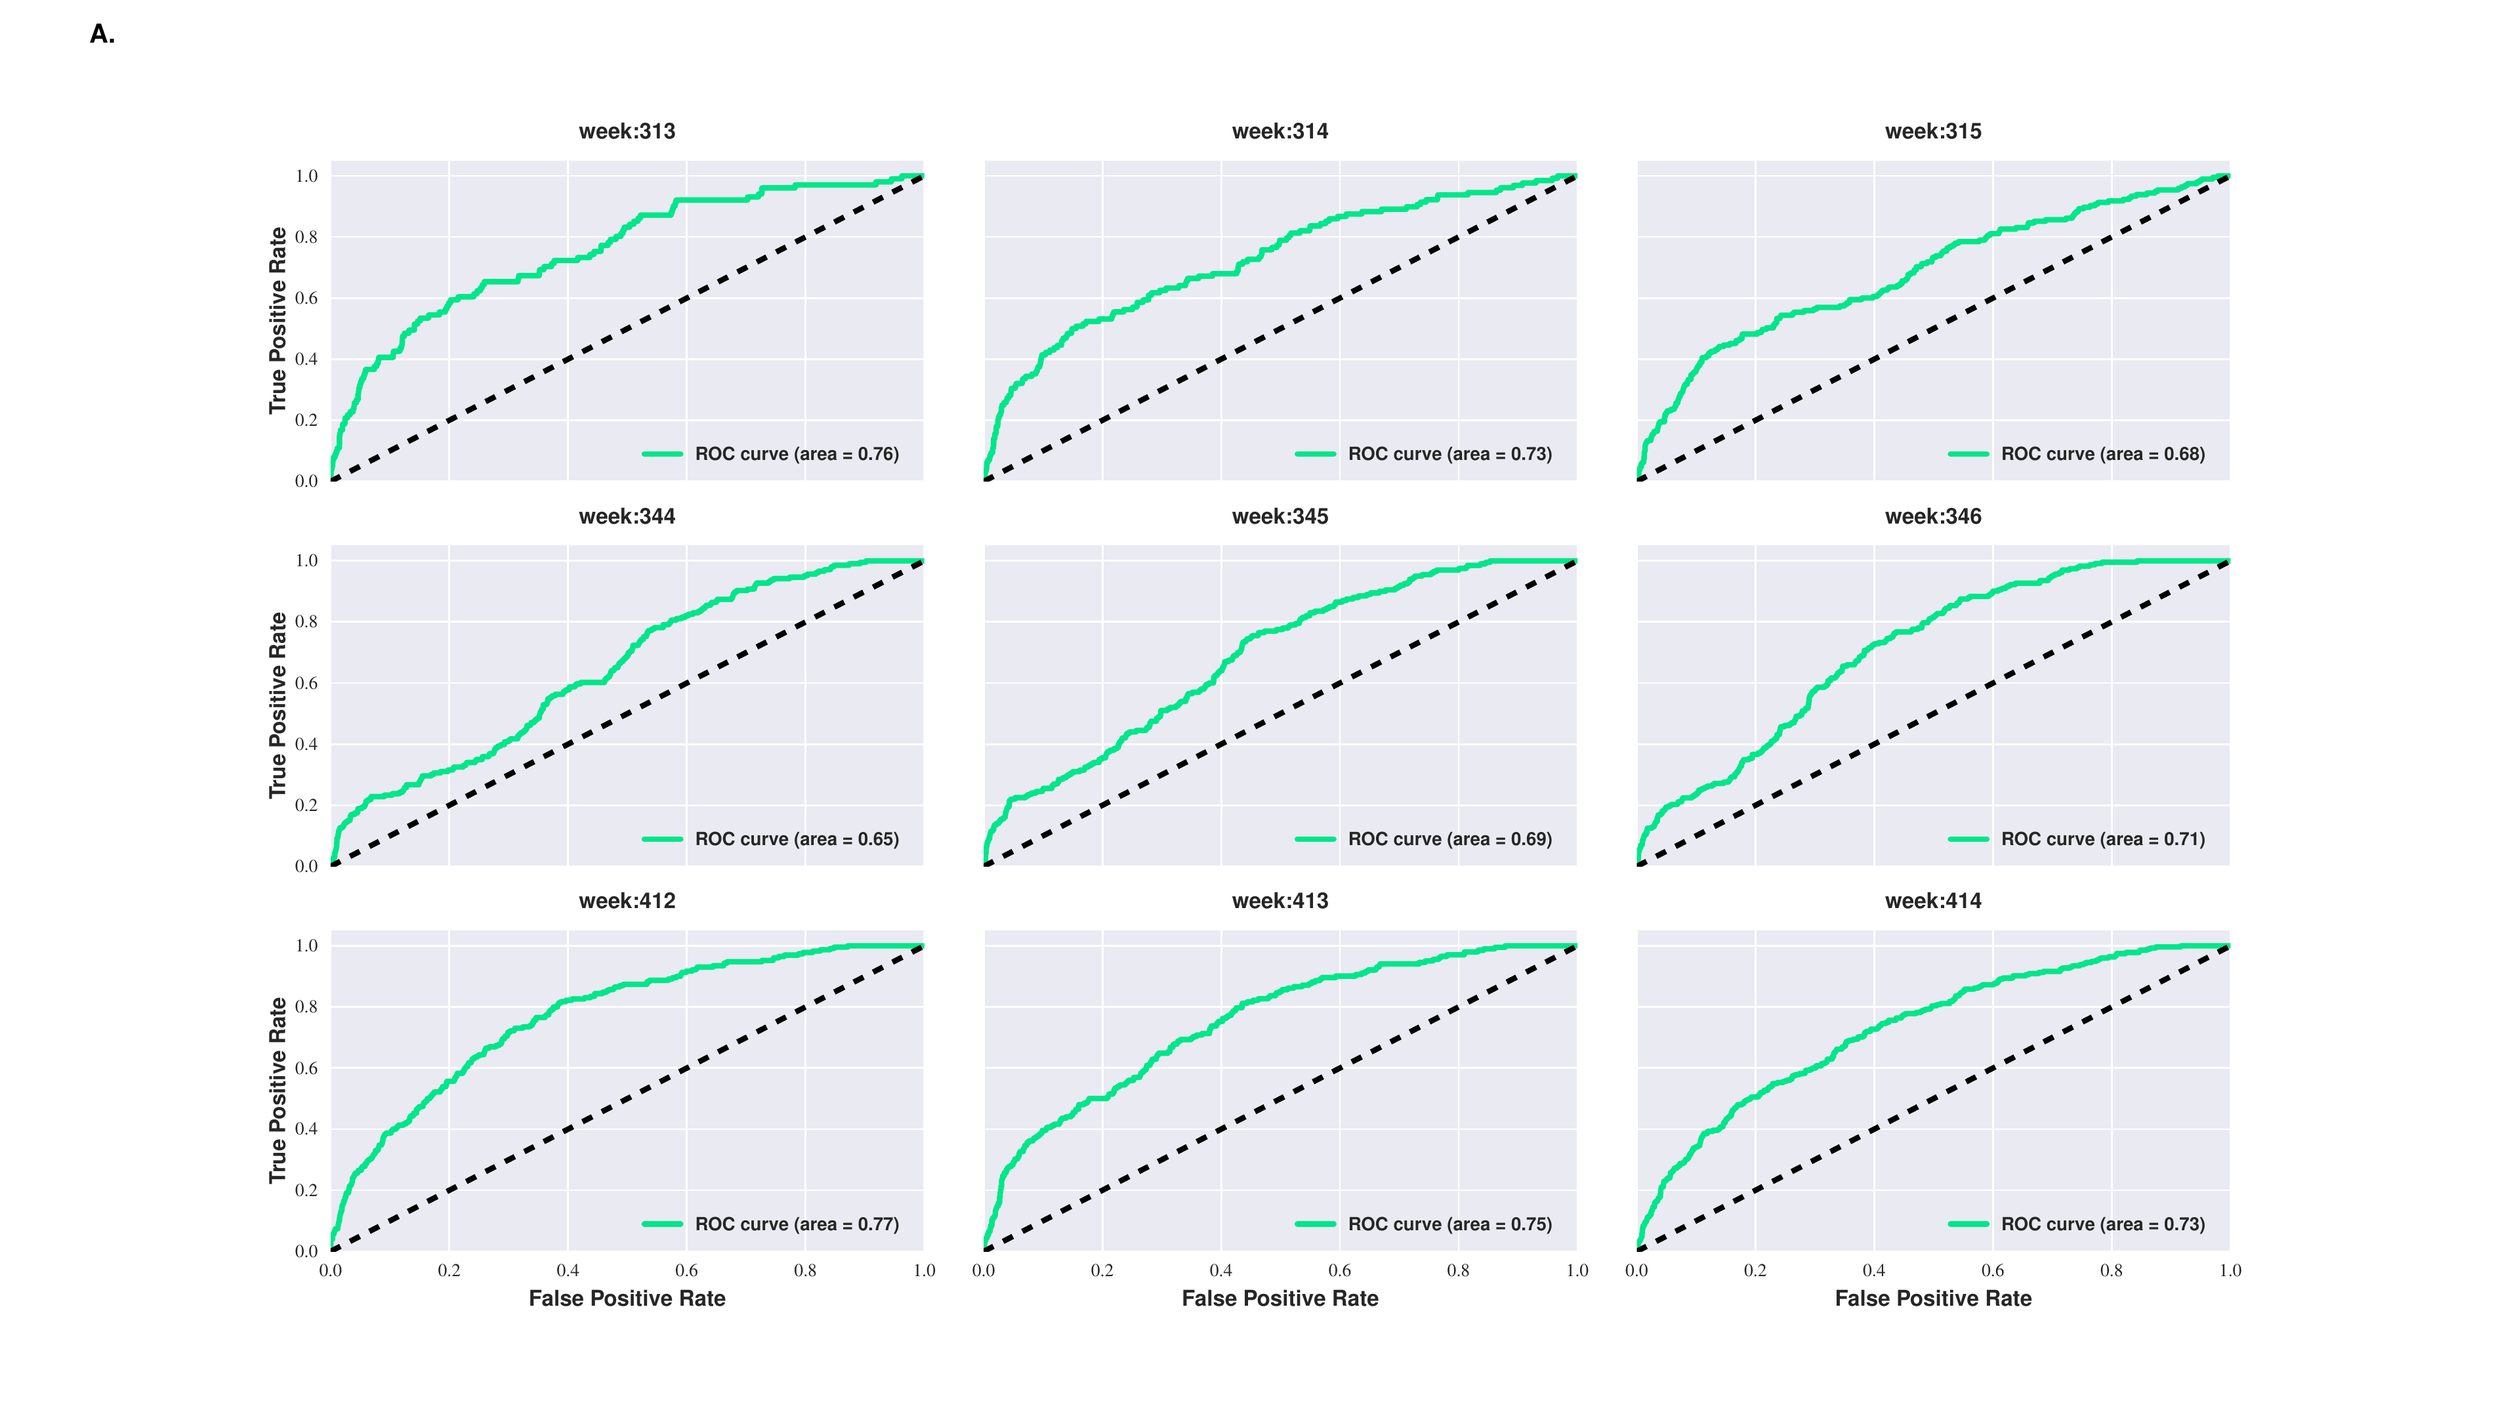
\begin{tikzpicture}[font=\bf\sffamily\fontsize{8}{8}\selectfont]
      \def\XST{-0.25in}
      \def\YST{0.25in}
      \node[] (A) {%% Creator: Matplotlib, PGF backend
%%
%% To include the figure in your LaTeX document, write
%%   \input{<filename>.pgf}
%%
%% Make sure the required packages are loaded in your preamble
%%   \usepackage{pgf}
%%
%% Figures using additional raster images can only be included by \input if
%% they are in the same directory as the main LaTeX file. For loading figures
%% from other directories you can use the `import` package
%%   \usepackage{import}
%% and then include the figures with
%%   \import{<path to file>}{<filename>.pgf}
%%
%% Matplotlib used the following preamble
%%   \usepackage[utf8x]{inputenc}
%%   \usepackage[T1]{fontenc}
%%
\begingroup%
\makeatletter%
\begin{pgfpicture}%
\pgfpathrectangle{\pgfpointorigin}{\pgfqpoint{18.679950in}{10.390360in}}%
\pgfusepath{use as bounding box, clip}%
\begin{pgfscope}%
\pgfsetbuttcap%
\pgfsetmiterjoin%
\definecolor{currentfill}{rgb}{1.000000,1.000000,1.000000}%
\pgfsetfillcolor{currentfill}%
\pgfsetlinewidth{0.000000pt}%
\definecolor{currentstroke}{rgb}{1.000000,1.000000,1.000000}%
\pgfsetstrokecolor{currentstroke}%
\pgfsetdash{}{0pt}%
\pgfpathmoveto{\pgfqpoint{0.000000in}{0.000000in}}%
\pgfpathlineto{\pgfqpoint{18.679950in}{0.000000in}}%
\pgfpathlineto{\pgfqpoint{18.679950in}{10.390360in}}%
\pgfpathlineto{\pgfqpoint{0.000000in}{10.390360in}}%
\pgfpathclose%
\pgfusepath{fill}%
\end{pgfscope}%
\begin{pgfscope}%
\pgfsetbuttcap%
\pgfsetmiterjoin%
\definecolor{currentfill}{rgb}{0.917647,0.917647,0.949020}%
\pgfsetfillcolor{currentfill}%
\pgfsetlinewidth{0.000000pt}%
\definecolor{currentstroke}{rgb}{0.000000,0.000000,0.000000}%
\pgfsetstrokecolor{currentstroke}%
\pgfsetstrokeopacity{0.000000}%
\pgfsetdash{}{0pt}%
\pgfpathmoveto{\pgfqpoint{2.334994in}{6.906533in}}%
\pgfpathlineto{\pgfqpoint{6.859044in}{6.906533in}}%
\pgfpathlineto{\pgfqpoint{6.859044in}{9.351324in}}%
\pgfpathlineto{\pgfqpoint{2.334994in}{9.351324in}}%
\pgfpathclose%
\pgfusepath{fill}%
\end{pgfscope}%
\begin{pgfscope}%
\pgfpathrectangle{\pgfqpoint{2.334994in}{6.906533in}}{\pgfqpoint{4.524050in}{2.444791in}} %
\pgfusepath{clip}%
\pgfsetroundcap%
\pgfsetroundjoin%
\pgfsetlinewidth{1.003750pt}%
\definecolor{currentstroke}{rgb}{1.000000,1.000000,1.000000}%
\pgfsetstrokecolor{currentstroke}%
\pgfsetdash{}{0pt}%
\pgfpathmoveto{\pgfqpoint{2.334994in}{6.906533in}}%
\pgfpathlineto{\pgfqpoint{2.334994in}{9.351324in}}%
\pgfusepath{stroke}%
\end{pgfscope}%
\begin{pgfscope}%
\pgfsetbuttcap%
\pgfsetroundjoin%
\definecolor{currentfill}{rgb}{0.150000,0.150000,0.150000}%
\pgfsetfillcolor{currentfill}%
\pgfsetlinewidth{1.003750pt}%
\definecolor{currentstroke}{rgb}{0.150000,0.150000,0.150000}%
\pgfsetstrokecolor{currentstroke}%
\pgfsetdash{}{0pt}%
\pgfsys@defobject{currentmarker}{\pgfqpoint{0.000000in}{0.000000in}}{\pgfqpoint{0.000000in}{0.000000in}}{%
\pgfpathmoveto{\pgfqpoint{0.000000in}{0.000000in}}%
\pgfpathlineto{\pgfqpoint{0.000000in}{0.000000in}}%
\pgfusepath{stroke,fill}%
}%
\begin{pgfscope}%
\pgfsys@transformshift{2.334994in}{6.906533in}%
\pgfsys@useobject{currentmarker}{}%
\end{pgfscope}%
\end{pgfscope}%
\begin{pgfscope}%
\pgfsetbuttcap%
\pgfsetroundjoin%
\definecolor{currentfill}{rgb}{0.150000,0.150000,0.150000}%
\pgfsetfillcolor{currentfill}%
\pgfsetlinewidth{1.003750pt}%
\definecolor{currentstroke}{rgb}{0.150000,0.150000,0.150000}%
\pgfsetstrokecolor{currentstroke}%
\pgfsetdash{}{0pt}%
\pgfsys@defobject{currentmarker}{\pgfqpoint{0.000000in}{0.000000in}}{\pgfqpoint{0.000000in}{0.000000in}}{%
\pgfpathmoveto{\pgfqpoint{0.000000in}{0.000000in}}%
\pgfpathlineto{\pgfqpoint{0.000000in}{0.000000in}}%
\pgfusepath{stroke,fill}%
}%
\begin{pgfscope}%
\pgfsys@transformshift{2.334994in}{9.351324in}%
\pgfsys@useobject{currentmarker}{}%
\end{pgfscope}%
\end{pgfscope}%
\begin{pgfscope}%
\pgfpathrectangle{\pgfqpoint{2.334994in}{6.906533in}}{\pgfqpoint{4.524050in}{2.444791in}} %
\pgfusepath{clip}%
\pgfsetroundcap%
\pgfsetroundjoin%
\pgfsetlinewidth{1.003750pt}%
\definecolor{currentstroke}{rgb}{1.000000,1.000000,1.000000}%
\pgfsetstrokecolor{currentstroke}%
\pgfsetdash{}{0pt}%
\pgfpathmoveto{\pgfqpoint{3.239804in}{6.906533in}}%
\pgfpathlineto{\pgfqpoint{3.239804in}{9.351324in}}%
\pgfusepath{stroke}%
\end{pgfscope}%
\begin{pgfscope}%
\pgfsetbuttcap%
\pgfsetroundjoin%
\definecolor{currentfill}{rgb}{0.150000,0.150000,0.150000}%
\pgfsetfillcolor{currentfill}%
\pgfsetlinewidth{1.003750pt}%
\definecolor{currentstroke}{rgb}{0.150000,0.150000,0.150000}%
\pgfsetstrokecolor{currentstroke}%
\pgfsetdash{}{0pt}%
\pgfsys@defobject{currentmarker}{\pgfqpoint{0.000000in}{0.000000in}}{\pgfqpoint{0.000000in}{0.000000in}}{%
\pgfpathmoveto{\pgfqpoint{0.000000in}{0.000000in}}%
\pgfpathlineto{\pgfqpoint{0.000000in}{0.000000in}}%
\pgfusepath{stroke,fill}%
}%
\begin{pgfscope}%
\pgfsys@transformshift{3.239804in}{6.906533in}%
\pgfsys@useobject{currentmarker}{}%
\end{pgfscope}%
\end{pgfscope}%
\begin{pgfscope}%
\pgfsetbuttcap%
\pgfsetroundjoin%
\definecolor{currentfill}{rgb}{0.150000,0.150000,0.150000}%
\pgfsetfillcolor{currentfill}%
\pgfsetlinewidth{1.003750pt}%
\definecolor{currentstroke}{rgb}{0.150000,0.150000,0.150000}%
\pgfsetstrokecolor{currentstroke}%
\pgfsetdash{}{0pt}%
\pgfsys@defobject{currentmarker}{\pgfqpoint{0.000000in}{0.000000in}}{\pgfqpoint{0.000000in}{0.000000in}}{%
\pgfpathmoveto{\pgfqpoint{0.000000in}{0.000000in}}%
\pgfpathlineto{\pgfqpoint{0.000000in}{0.000000in}}%
\pgfusepath{stroke,fill}%
}%
\begin{pgfscope}%
\pgfsys@transformshift{3.239804in}{9.351324in}%
\pgfsys@useobject{currentmarker}{}%
\end{pgfscope}%
\end{pgfscope}%
\begin{pgfscope}%
\pgfpathrectangle{\pgfqpoint{2.334994in}{6.906533in}}{\pgfqpoint{4.524050in}{2.444791in}} %
\pgfusepath{clip}%
\pgfsetroundcap%
\pgfsetroundjoin%
\pgfsetlinewidth{1.003750pt}%
\definecolor{currentstroke}{rgb}{1.000000,1.000000,1.000000}%
\pgfsetstrokecolor{currentstroke}%
\pgfsetdash{}{0pt}%
\pgfpathmoveto{\pgfqpoint{4.144614in}{6.906533in}}%
\pgfpathlineto{\pgfqpoint{4.144614in}{9.351324in}}%
\pgfusepath{stroke}%
\end{pgfscope}%
\begin{pgfscope}%
\pgfsetbuttcap%
\pgfsetroundjoin%
\definecolor{currentfill}{rgb}{0.150000,0.150000,0.150000}%
\pgfsetfillcolor{currentfill}%
\pgfsetlinewidth{1.003750pt}%
\definecolor{currentstroke}{rgb}{0.150000,0.150000,0.150000}%
\pgfsetstrokecolor{currentstroke}%
\pgfsetdash{}{0pt}%
\pgfsys@defobject{currentmarker}{\pgfqpoint{0.000000in}{0.000000in}}{\pgfqpoint{0.000000in}{0.000000in}}{%
\pgfpathmoveto{\pgfqpoint{0.000000in}{0.000000in}}%
\pgfpathlineto{\pgfqpoint{0.000000in}{0.000000in}}%
\pgfusepath{stroke,fill}%
}%
\begin{pgfscope}%
\pgfsys@transformshift{4.144614in}{6.906533in}%
\pgfsys@useobject{currentmarker}{}%
\end{pgfscope}%
\end{pgfscope}%
\begin{pgfscope}%
\pgfsetbuttcap%
\pgfsetroundjoin%
\definecolor{currentfill}{rgb}{0.150000,0.150000,0.150000}%
\pgfsetfillcolor{currentfill}%
\pgfsetlinewidth{1.003750pt}%
\definecolor{currentstroke}{rgb}{0.150000,0.150000,0.150000}%
\pgfsetstrokecolor{currentstroke}%
\pgfsetdash{}{0pt}%
\pgfsys@defobject{currentmarker}{\pgfqpoint{0.000000in}{0.000000in}}{\pgfqpoint{0.000000in}{0.000000in}}{%
\pgfpathmoveto{\pgfqpoint{0.000000in}{0.000000in}}%
\pgfpathlineto{\pgfqpoint{0.000000in}{0.000000in}}%
\pgfusepath{stroke,fill}%
}%
\begin{pgfscope}%
\pgfsys@transformshift{4.144614in}{9.351324in}%
\pgfsys@useobject{currentmarker}{}%
\end{pgfscope}%
\end{pgfscope}%
\begin{pgfscope}%
\pgfpathrectangle{\pgfqpoint{2.334994in}{6.906533in}}{\pgfqpoint{4.524050in}{2.444791in}} %
\pgfusepath{clip}%
\pgfsetroundcap%
\pgfsetroundjoin%
\pgfsetlinewidth{1.003750pt}%
\definecolor{currentstroke}{rgb}{1.000000,1.000000,1.000000}%
\pgfsetstrokecolor{currentstroke}%
\pgfsetdash{}{0pt}%
\pgfpathmoveto{\pgfqpoint{5.049424in}{6.906533in}}%
\pgfpathlineto{\pgfqpoint{5.049424in}{9.351324in}}%
\pgfusepath{stroke}%
\end{pgfscope}%
\begin{pgfscope}%
\pgfsetbuttcap%
\pgfsetroundjoin%
\definecolor{currentfill}{rgb}{0.150000,0.150000,0.150000}%
\pgfsetfillcolor{currentfill}%
\pgfsetlinewidth{1.003750pt}%
\definecolor{currentstroke}{rgb}{0.150000,0.150000,0.150000}%
\pgfsetstrokecolor{currentstroke}%
\pgfsetdash{}{0pt}%
\pgfsys@defobject{currentmarker}{\pgfqpoint{0.000000in}{0.000000in}}{\pgfqpoint{0.000000in}{0.000000in}}{%
\pgfpathmoveto{\pgfqpoint{0.000000in}{0.000000in}}%
\pgfpathlineto{\pgfqpoint{0.000000in}{0.000000in}}%
\pgfusepath{stroke,fill}%
}%
\begin{pgfscope}%
\pgfsys@transformshift{5.049424in}{6.906533in}%
\pgfsys@useobject{currentmarker}{}%
\end{pgfscope}%
\end{pgfscope}%
\begin{pgfscope}%
\pgfsetbuttcap%
\pgfsetroundjoin%
\definecolor{currentfill}{rgb}{0.150000,0.150000,0.150000}%
\pgfsetfillcolor{currentfill}%
\pgfsetlinewidth{1.003750pt}%
\definecolor{currentstroke}{rgb}{0.150000,0.150000,0.150000}%
\pgfsetstrokecolor{currentstroke}%
\pgfsetdash{}{0pt}%
\pgfsys@defobject{currentmarker}{\pgfqpoint{0.000000in}{0.000000in}}{\pgfqpoint{0.000000in}{0.000000in}}{%
\pgfpathmoveto{\pgfqpoint{0.000000in}{0.000000in}}%
\pgfpathlineto{\pgfqpoint{0.000000in}{0.000000in}}%
\pgfusepath{stroke,fill}%
}%
\begin{pgfscope}%
\pgfsys@transformshift{5.049424in}{9.351324in}%
\pgfsys@useobject{currentmarker}{}%
\end{pgfscope}%
\end{pgfscope}%
\begin{pgfscope}%
\pgfpathrectangle{\pgfqpoint{2.334994in}{6.906533in}}{\pgfqpoint{4.524050in}{2.444791in}} %
\pgfusepath{clip}%
\pgfsetroundcap%
\pgfsetroundjoin%
\pgfsetlinewidth{1.003750pt}%
\definecolor{currentstroke}{rgb}{1.000000,1.000000,1.000000}%
\pgfsetstrokecolor{currentstroke}%
\pgfsetdash{}{0pt}%
\pgfpathmoveto{\pgfqpoint{5.954234in}{6.906533in}}%
\pgfpathlineto{\pgfqpoint{5.954234in}{9.351324in}}%
\pgfusepath{stroke}%
\end{pgfscope}%
\begin{pgfscope}%
\pgfsetbuttcap%
\pgfsetroundjoin%
\definecolor{currentfill}{rgb}{0.150000,0.150000,0.150000}%
\pgfsetfillcolor{currentfill}%
\pgfsetlinewidth{1.003750pt}%
\definecolor{currentstroke}{rgb}{0.150000,0.150000,0.150000}%
\pgfsetstrokecolor{currentstroke}%
\pgfsetdash{}{0pt}%
\pgfsys@defobject{currentmarker}{\pgfqpoint{0.000000in}{0.000000in}}{\pgfqpoint{0.000000in}{0.000000in}}{%
\pgfpathmoveto{\pgfqpoint{0.000000in}{0.000000in}}%
\pgfpathlineto{\pgfqpoint{0.000000in}{0.000000in}}%
\pgfusepath{stroke,fill}%
}%
\begin{pgfscope}%
\pgfsys@transformshift{5.954234in}{6.906533in}%
\pgfsys@useobject{currentmarker}{}%
\end{pgfscope}%
\end{pgfscope}%
\begin{pgfscope}%
\pgfsetbuttcap%
\pgfsetroundjoin%
\definecolor{currentfill}{rgb}{0.150000,0.150000,0.150000}%
\pgfsetfillcolor{currentfill}%
\pgfsetlinewidth{1.003750pt}%
\definecolor{currentstroke}{rgb}{0.150000,0.150000,0.150000}%
\pgfsetstrokecolor{currentstroke}%
\pgfsetdash{}{0pt}%
\pgfsys@defobject{currentmarker}{\pgfqpoint{0.000000in}{0.000000in}}{\pgfqpoint{0.000000in}{0.000000in}}{%
\pgfpathmoveto{\pgfqpoint{0.000000in}{0.000000in}}%
\pgfpathlineto{\pgfqpoint{0.000000in}{0.000000in}}%
\pgfusepath{stroke,fill}%
}%
\begin{pgfscope}%
\pgfsys@transformshift{5.954234in}{9.351324in}%
\pgfsys@useobject{currentmarker}{}%
\end{pgfscope}%
\end{pgfscope}%
\begin{pgfscope}%
\pgfpathrectangle{\pgfqpoint{2.334994in}{6.906533in}}{\pgfqpoint{4.524050in}{2.444791in}} %
\pgfusepath{clip}%
\pgfsetroundcap%
\pgfsetroundjoin%
\pgfsetlinewidth{1.003750pt}%
\definecolor{currentstroke}{rgb}{1.000000,1.000000,1.000000}%
\pgfsetstrokecolor{currentstroke}%
\pgfsetdash{}{0pt}%
\pgfpathmoveto{\pgfqpoint{6.859044in}{6.906533in}}%
\pgfpathlineto{\pgfqpoint{6.859044in}{9.351324in}}%
\pgfusepath{stroke}%
\end{pgfscope}%
\begin{pgfscope}%
\pgfsetbuttcap%
\pgfsetroundjoin%
\definecolor{currentfill}{rgb}{0.150000,0.150000,0.150000}%
\pgfsetfillcolor{currentfill}%
\pgfsetlinewidth{1.003750pt}%
\definecolor{currentstroke}{rgb}{0.150000,0.150000,0.150000}%
\pgfsetstrokecolor{currentstroke}%
\pgfsetdash{}{0pt}%
\pgfsys@defobject{currentmarker}{\pgfqpoint{0.000000in}{0.000000in}}{\pgfqpoint{0.000000in}{0.000000in}}{%
\pgfpathmoveto{\pgfqpoint{0.000000in}{0.000000in}}%
\pgfpathlineto{\pgfqpoint{0.000000in}{0.000000in}}%
\pgfusepath{stroke,fill}%
}%
\begin{pgfscope}%
\pgfsys@transformshift{6.859044in}{6.906533in}%
\pgfsys@useobject{currentmarker}{}%
\end{pgfscope}%
\end{pgfscope}%
\begin{pgfscope}%
\pgfsetbuttcap%
\pgfsetroundjoin%
\definecolor{currentfill}{rgb}{0.150000,0.150000,0.150000}%
\pgfsetfillcolor{currentfill}%
\pgfsetlinewidth{1.003750pt}%
\definecolor{currentstroke}{rgb}{0.150000,0.150000,0.150000}%
\pgfsetstrokecolor{currentstroke}%
\pgfsetdash{}{0pt}%
\pgfsys@defobject{currentmarker}{\pgfqpoint{0.000000in}{0.000000in}}{\pgfqpoint{0.000000in}{0.000000in}}{%
\pgfpathmoveto{\pgfqpoint{0.000000in}{0.000000in}}%
\pgfpathlineto{\pgfqpoint{0.000000in}{0.000000in}}%
\pgfusepath{stroke,fill}%
}%
\begin{pgfscope}%
\pgfsys@transformshift{6.859044in}{9.351324in}%
\pgfsys@useobject{currentmarker}{}%
\end{pgfscope}%
\end{pgfscope}%
\begin{pgfscope}%
\pgfpathrectangle{\pgfqpoint{2.334994in}{6.906533in}}{\pgfqpoint{4.524050in}{2.444791in}} %
\pgfusepath{clip}%
\pgfsetroundcap%
\pgfsetroundjoin%
\pgfsetlinewidth{1.003750pt}%
\definecolor{currentstroke}{rgb}{1.000000,1.000000,1.000000}%
\pgfsetstrokecolor{currentstroke}%
\pgfsetdash{}{0pt}%
\pgfpathmoveto{\pgfqpoint{2.334994in}{6.906533in}}%
\pgfpathlineto{\pgfqpoint{6.859044in}{6.906533in}}%
\pgfusepath{stroke}%
\end{pgfscope}%
\begin{pgfscope}%
\pgfsetbuttcap%
\pgfsetroundjoin%
\definecolor{currentfill}{rgb}{0.150000,0.150000,0.150000}%
\pgfsetfillcolor{currentfill}%
\pgfsetlinewidth{1.003750pt}%
\definecolor{currentstroke}{rgb}{0.150000,0.150000,0.150000}%
\pgfsetstrokecolor{currentstroke}%
\pgfsetdash{}{0pt}%
\pgfsys@defobject{currentmarker}{\pgfqpoint{0.000000in}{0.000000in}}{\pgfqpoint{0.000000in}{0.000000in}}{%
\pgfpathmoveto{\pgfqpoint{0.000000in}{0.000000in}}%
\pgfpathlineto{\pgfqpoint{0.000000in}{0.000000in}}%
\pgfusepath{stroke,fill}%
}%
\begin{pgfscope}%
\pgfsys@transformshift{2.334994in}{6.906533in}%
\pgfsys@useobject{currentmarker}{}%
\end{pgfscope}%
\end{pgfscope}%
\begin{pgfscope}%
\pgfsetbuttcap%
\pgfsetroundjoin%
\definecolor{currentfill}{rgb}{0.150000,0.150000,0.150000}%
\pgfsetfillcolor{currentfill}%
\pgfsetlinewidth{1.003750pt}%
\definecolor{currentstroke}{rgb}{0.150000,0.150000,0.150000}%
\pgfsetstrokecolor{currentstroke}%
\pgfsetdash{}{0pt}%
\pgfsys@defobject{currentmarker}{\pgfqpoint{0.000000in}{0.000000in}}{\pgfqpoint{0.000000in}{0.000000in}}{%
\pgfpathmoveto{\pgfqpoint{0.000000in}{0.000000in}}%
\pgfpathlineto{\pgfqpoint{0.000000in}{0.000000in}}%
\pgfusepath{stroke,fill}%
}%
\begin{pgfscope}%
\pgfsys@transformshift{6.859044in}{6.906533in}%
\pgfsys@useobject{currentmarker}{}%
\end{pgfscope}%
\end{pgfscope}%
\begin{pgfscope}%
\definecolor{textcolor}{rgb}{0.150000,0.150000,0.150000}%
\pgfsetstrokecolor{textcolor}%
\pgfsetfillcolor{textcolor}%
\pgftext[x=2.237772in,y=6.906533in,right,]{\color{textcolor}\sffamily\fontsize{10.000000}{12.000000}\bfseries\selectfont \(\displaystyle 0.0\)}%
\end{pgfscope}%
\begin{pgfscope}%
\pgfpathrectangle{\pgfqpoint{2.334994in}{6.906533in}}{\pgfqpoint{4.524050in}{2.444791in}} %
\pgfusepath{clip}%
\pgfsetroundcap%
\pgfsetroundjoin%
\pgfsetlinewidth{1.003750pt}%
\definecolor{currentstroke}{rgb}{1.000000,1.000000,1.000000}%
\pgfsetstrokecolor{currentstroke}%
\pgfsetdash{}{0pt}%
\pgfpathmoveto{\pgfqpoint{2.334994in}{7.372208in}}%
\pgfpathlineto{\pgfqpoint{6.859044in}{7.372208in}}%
\pgfusepath{stroke}%
\end{pgfscope}%
\begin{pgfscope}%
\pgfsetbuttcap%
\pgfsetroundjoin%
\definecolor{currentfill}{rgb}{0.150000,0.150000,0.150000}%
\pgfsetfillcolor{currentfill}%
\pgfsetlinewidth{1.003750pt}%
\definecolor{currentstroke}{rgb}{0.150000,0.150000,0.150000}%
\pgfsetstrokecolor{currentstroke}%
\pgfsetdash{}{0pt}%
\pgfsys@defobject{currentmarker}{\pgfqpoint{0.000000in}{0.000000in}}{\pgfqpoint{0.000000in}{0.000000in}}{%
\pgfpathmoveto{\pgfqpoint{0.000000in}{0.000000in}}%
\pgfpathlineto{\pgfqpoint{0.000000in}{0.000000in}}%
\pgfusepath{stroke,fill}%
}%
\begin{pgfscope}%
\pgfsys@transformshift{2.334994in}{7.372208in}%
\pgfsys@useobject{currentmarker}{}%
\end{pgfscope}%
\end{pgfscope}%
\begin{pgfscope}%
\pgfsetbuttcap%
\pgfsetroundjoin%
\definecolor{currentfill}{rgb}{0.150000,0.150000,0.150000}%
\pgfsetfillcolor{currentfill}%
\pgfsetlinewidth{1.003750pt}%
\definecolor{currentstroke}{rgb}{0.150000,0.150000,0.150000}%
\pgfsetstrokecolor{currentstroke}%
\pgfsetdash{}{0pt}%
\pgfsys@defobject{currentmarker}{\pgfqpoint{0.000000in}{0.000000in}}{\pgfqpoint{0.000000in}{0.000000in}}{%
\pgfpathmoveto{\pgfqpoint{0.000000in}{0.000000in}}%
\pgfpathlineto{\pgfqpoint{0.000000in}{0.000000in}}%
\pgfusepath{stroke,fill}%
}%
\begin{pgfscope}%
\pgfsys@transformshift{6.859044in}{7.372208in}%
\pgfsys@useobject{currentmarker}{}%
\end{pgfscope}%
\end{pgfscope}%
\begin{pgfscope}%
\definecolor{textcolor}{rgb}{0.150000,0.150000,0.150000}%
\pgfsetstrokecolor{textcolor}%
\pgfsetfillcolor{textcolor}%
\pgftext[x=2.237772in,y=7.372208in,right,]{\color{textcolor}\sffamily\fontsize{10.000000}{12.000000}\bfseries\selectfont \(\displaystyle 0.2\)}%
\end{pgfscope}%
\begin{pgfscope}%
\pgfpathrectangle{\pgfqpoint{2.334994in}{6.906533in}}{\pgfqpoint{4.524050in}{2.444791in}} %
\pgfusepath{clip}%
\pgfsetroundcap%
\pgfsetroundjoin%
\pgfsetlinewidth{1.003750pt}%
\definecolor{currentstroke}{rgb}{1.000000,1.000000,1.000000}%
\pgfsetstrokecolor{currentstroke}%
\pgfsetdash{}{0pt}%
\pgfpathmoveto{\pgfqpoint{2.334994in}{7.837882in}}%
\pgfpathlineto{\pgfqpoint{6.859044in}{7.837882in}}%
\pgfusepath{stroke}%
\end{pgfscope}%
\begin{pgfscope}%
\pgfsetbuttcap%
\pgfsetroundjoin%
\definecolor{currentfill}{rgb}{0.150000,0.150000,0.150000}%
\pgfsetfillcolor{currentfill}%
\pgfsetlinewidth{1.003750pt}%
\definecolor{currentstroke}{rgb}{0.150000,0.150000,0.150000}%
\pgfsetstrokecolor{currentstroke}%
\pgfsetdash{}{0pt}%
\pgfsys@defobject{currentmarker}{\pgfqpoint{0.000000in}{0.000000in}}{\pgfqpoint{0.000000in}{0.000000in}}{%
\pgfpathmoveto{\pgfqpoint{0.000000in}{0.000000in}}%
\pgfpathlineto{\pgfqpoint{0.000000in}{0.000000in}}%
\pgfusepath{stroke,fill}%
}%
\begin{pgfscope}%
\pgfsys@transformshift{2.334994in}{7.837882in}%
\pgfsys@useobject{currentmarker}{}%
\end{pgfscope}%
\end{pgfscope}%
\begin{pgfscope}%
\pgfsetbuttcap%
\pgfsetroundjoin%
\definecolor{currentfill}{rgb}{0.150000,0.150000,0.150000}%
\pgfsetfillcolor{currentfill}%
\pgfsetlinewidth{1.003750pt}%
\definecolor{currentstroke}{rgb}{0.150000,0.150000,0.150000}%
\pgfsetstrokecolor{currentstroke}%
\pgfsetdash{}{0pt}%
\pgfsys@defobject{currentmarker}{\pgfqpoint{0.000000in}{0.000000in}}{\pgfqpoint{0.000000in}{0.000000in}}{%
\pgfpathmoveto{\pgfqpoint{0.000000in}{0.000000in}}%
\pgfpathlineto{\pgfqpoint{0.000000in}{0.000000in}}%
\pgfusepath{stroke,fill}%
}%
\begin{pgfscope}%
\pgfsys@transformshift{6.859044in}{7.837882in}%
\pgfsys@useobject{currentmarker}{}%
\end{pgfscope}%
\end{pgfscope}%
\begin{pgfscope}%
\definecolor{textcolor}{rgb}{0.150000,0.150000,0.150000}%
\pgfsetstrokecolor{textcolor}%
\pgfsetfillcolor{textcolor}%
\pgftext[x=2.237772in,y=7.837882in,right,]{\color{textcolor}\sffamily\fontsize{10.000000}{12.000000}\bfseries\selectfont \(\displaystyle 0.4\)}%
\end{pgfscope}%
\begin{pgfscope}%
\pgfpathrectangle{\pgfqpoint{2.334994in}{6.906533in}}{\pgfqpoint{4.524050in}{2.444791in}} %
\pgfusepath{clip}%
\pgfsetroundcap%
\pgfsetroundjoin%
\pgfsetlinewidth{1.003750pt}%
\definecolor{currentstroke}{rgb}{1.000000,1.000000,1.000000}%
\pgfsetstrokecolor{currentstroke}%
\pgfsetdash{}{0pt}%
\pgfpathmoveto{\pgfqpoint{2.334994in}{8.303556in}}%
\pgfpathlineto{\pgfqpoint{6.859044in}{8.303556in}}%
\pgfusepath{stroke}%
\end{pgfscope}%
\begin{pgfscope}%
\pgfsetbuttcap%
\pgfsetroundjoin%
\definecolor{currentfill}{rgb}{0.150000,0.150000,0.150000}%
\pgfsetfillcolor{currentfill}%
\pgfsetlinewidth{1.003750pt}%
\definecolor{currentstroke}{rgb}{0.150000,0.150000,0.150000}%
\pgfsetstrokecolor{currentstroke}%
\pgfsetdash{}{0pt}%
\pgfsys@defobject{currentmarker}{\pgfqpoint{0.000000in}{0.000000in}}{\pgfqpoint{0.000000in}{0.000000in}}{%
\pgfpathmoveto{\pgfqpoint{0.000000in}{0.000000in}}%
\pgfpathlineto{\pgfqpoint{0.000000in}{0.000000in}}%
\pgfusepath{stroke,fill}%
}%
\begin{pgfscope}%
\pgfsys@transformshift{2.334994in}{8.303556in}%
\pgfsys@useobject{currentmarker}{}%
\end{pgfscope}%
\end{pgfscope}%
\begin{pgfscope}%
\pgfsetbuttcap%
\pgfsetroundjoin%
\definecolor{currentfill}{rgb}{0.150000,0.150000,0.150000}%
\pgfsetfillcolor{currentfill}%
\pgfsetlinewidth{1.003750pt}%
\definecolor{currentstroke}{rgb}{0.150000,0.150000,0.150000}%
\pgfsetstrokecolor{currentstroke}%
\pgfsetdash{}{0pt}%
\pgfsys@defobject{currentmarker}{\pgfqpoint{0.000000in}{0.000000in}}{\pgfqpoint{0.000000in}{0.000000in}}{%
\pgfpathmoveto{\pgfqpoint{0.000000in}{0.000000in}}%
\pgfpathlineto{\pgfqpoint{0.000000in}{0.000000in}}%
\pgfusepath{stroke,fill}%
}%
\begin{pgfscope}%
\pgfsys@transformshift{6.859044in}{8.303556in}%
\pgfsys@useobject{currentmarker}{}%
\end{pgfscope}%
\end{pgfscope}%
\begin{pgfscope}%
\definecolor{textcolor}{rgb}{0.150000,0.150000,0.150000}%
\pgfsetstrokecolor{textcolor}%
\pgfsetfillcolor{textcolor}%
\pgftext[x=2.237772in,y=8.303556in,right,]{\color{textcolor}\sffamily\fontsize{10.000000}{12.000000}\bfseries\selectfont \(\displaystyle 0.6\)}%
\end{pgfscope}%
\begin{pgfscope}%
\pgfpathrectangle{\pgfqpoint{2.334994in}{6.906533in}}{\pgfqpoint{4.524050in}{2.444791in}} %
\pgfusepath{clip}%
\pgfsetroundcap%
\pgfsetroundjoin%
\pgfsetlinewidth{1.003750pt}%
\definecolor{currentstroke}{rgb}{1.000000,1.000000,1.000000}%
\pgfsetstrokecolor{currentstroke}%
\pgfsetdash{}{0pt}%
\pgfpathmoveto{\pgfqpoint{2.334994in}{8.769231in}}%
\pgfpathlineto{\pgfqpoint{6.859044in}{8.769231in}}%
\pgfusepath{stroke}%
\end{pgfscope}%
\begin{pgfscope}%
\pgfsetbuttcap%
\pgfsetroundjoin%
\definecolor{currentfill}{rgb}{0.150000,0.150000,0.150000}%
\pgfsetfillcolor{currentfill}%
\pgfsetlinewidth{1.003750pt}%
\definecolor{currentstroke}{rgb}{0.150000,0.150000,0.150000}%
\pgfsetstrokecolor{currentstroke}%
\pgfsetdash{}{0pt}%
\pgfsys@defobject{currentmarker}{\pgfqpoint{0.000000in}{0.000000in}}{\pgfqpoint{0.000000in}{0.000000in}}{%
\pgfpathmoveto{\pgfqpoint{0.000000in}{0.000000in}}%
\pgfpathlineto{\pgfqpoint{0.000000in}{0.000000in}}%
\pgfusepath{stroke,fill}%
}%
\begin{pgfscope}%
\pgfsys@transformshift{2.334994in}{8.769231in}%
\pgfsys@useobject{currentmarker}{}%
\end{pgfscope}%
\end{pgfscope}%
\begin{pgfscope}%
\pgfsetbuttcap%
\pgfsetroundjoin%
\definecolor{currentfill}{rgb}{0.150000,0.150000,0.150000}%
\pgfsetfillcolor{currentfill}%
\pgfsetlinewidth{1.003750pt}%
\definecolor{currentstroke}{rgb}{0.150000,0.150000,0.150000}%
\pgfsetstrokecolor{currentstroke}%
\pgfsetdash{}{0pt}%
\pgfsys@defobject{currentmarker}{\pgfqpoint{0.000000in}{0.000000in}}{\pgfqpoint{0.000000in}{0.000000in}}{%
\pgfpathmoveto{\pgfqpoint{0.000000in}{0.000000in}}%
\pgfpathlineto{\pgfqpoint{0.000000in}{0.000000in}}%
\pgfusepath{stroke,fill}%
}%
\begin{pgfscope}%
\pgfsys@transformshift{6.859044in}{8.769231in}%
\pgfsys@useobject{currentmarker}{}%
\end{pgfscope}%
\end{pgfscope}%
\begin{pgfscope}%
\definecolor{textcolor}{rgb}{0.150000,0.150000,0.150000}%
\pgfsetstrokecolor{textcolor}%
\pgfsetfillcolor{textcolor}%
\pgftext[x=2.237772in,y=8.769231in,right,]{\color{textcolor}\sffamily\fontsize{10.000000}{12.000000}\bfseries\selectfont \(\displaystyle 0.8\)}%
\end{pgfscope}%
\begin{pgfscope}%
\pgfpathrectangle{\pgfqpoint{2.334994in}{6.906533in}}{\pgfqpoint{4.524050in}{2.444791in}} %
\pgfusepath{clip}%
\pgfsetroundcap%
\pgfsetroundjoin%
\pgfsetlinewidth{1.003750pt}%
\definecolor{currentstroke}{rgb}{1.000000,1.000000,1.000000}%
\pgfsetstrokecolor{currentstroke}%
\pgfsetdash{}{0pt}%
\pgfpathmoveto{\pgfqpoint{2.334994in}{9.234905in}}%
\pgfpathlineto{\pgfqpoint{6.859044in}{9.234905in}}%
\pgfusepath{stroke}%
\end{pgfscope}%
\begin{pgfscope}%
\pgfsetbuttcap%
\pgfsetroundjoin%
\definecolor{currentfill}{rgb}{0.150000,0.150000,0.150000}%
\pgfsetfillcolor{currentfill}%
\pgfsetlinewidth{1.003750pt}%
\definecolor{currentstroke}{rgb}{0.150000,0.150000,0.150000}%
\pgfsetstrokecolor{currentstroke}%
\pgfsetdash{}{0pt}%
\pgfsys@defobject{currentmarker}{\pgfqpoint{0.000000in}{0.000000in}}{\pgfqpoint{0.000000in}{0.000000in}}{%
\pgfpathmoveto{\pgfqpoint{0.000000in}{0.000000in}}%
\pgfpathlineto{\pgfqpoint{0.000000in}{0.000000in}}%
\pgfusepath{stroke,fill}%
}%
\begin{pgfscope}%
\pgfsys@transformshift{2.334994in}{9.234905in}%
\pgfsys@useobject{currentmarker}{}%
\end{pgfscope}%
\end{pgfscope}%
\begin{pgfscope}%
\pgfsetbuttcap%
\pgfsetroundjoin%
\definecolor{currentfill}{rgb}{0.150000,0.150000,0.150000}%
\pgfsetfillcolor{currentfill}%
\pgfsetlinewidth{1.003750pt}%
\definecolor{currentstroke}{rgb}{0.150000,0.150000,0.150000}%
\pgfsetstrokecolor{currentstroke}%
\pgfsetdash{}{0pt}%
\pgfsys@defobject{currentmarker}{\pgfqpoint{0.000000in}{0.000000in}}{\pgfqpoint{0.000000in}{0.000000in}}{%
\pgfpathmoveto{\pgfqpoint{0.000000in}{0.000000in}}%
\pgfpathlineto{\pgfqpoint{0.000000in}{0.000000in}}%
\pgfusepath{stroke,fill}%
}%
\begin{pgfscope}%
\pgfsys@transformshift{6.859044in}{9.234905in}%
\pgfsys@useobject{currentmarker}{}%
\end{pgfscope}%
\end{pgfscope}%
\begin{pgfscope}%
\definecolor{textcolor}{rgb}{0.150000,0.150000,0.150000}%
\pgfsetstrokecolor{textcolor}%
\pgfsetfillcolor{textcolor}%
\pgftext[x=2.237772in,y=9.234905in,right,]{\color{textcolor}\sffamily\fontsize{10.000000}{12.000000}\bfseries\selectfont \(\displaystyle 1.0\)}%
\end{pgfscope}%
\begin{pgfscope}%
\definecolor{textcolor}{rgb}{0.150000,0.150000,0.150000}%
\pgfsetstrokecolor{textcolor}%
\pgfsetfillcolor{textcolor}%
\pgftext[x=1.990857in,y=8.128928in,,bottom,rotate=90.000000]{\color{textcolor}\sffamily\fontsize{12.000000}{14.400000}\bfseries\selectfont True Positive Rate}%
\end{pgfscope}%
\begin{pgfscope}%
\pgfpathrectangle{\pgfqpoint{2.334994in}{6.906533in}}{\pgfqpoint{4.524050in}{2.444791in}} %
\pgfusepath{clip}%
\pgfsetroundcap%
\pgfsetroundjoin%
\pgfsetlinewidth{3.011250pt}%
\definecolor{currentstroke}{rgb}{0.000000,0.901961,0.541176}%
\pgfsetstrokecolor{currentstroke}%
\pgfsetdash{}{0pt}%
\pgfpathmoveto{\pgfqpoint{2.334994in}{6.929586in}}%
\pgfpathlineto{\pgfqpoint{2.336528in}{6.929586in}}%
\pgfpathlineto{\pgfqpoint{2.336528in}{6.952640in}}%
\pgfpathlineto{\pgfqpoint{2.338062in}{6.952640in}}%
\pgfpathlineto{\pgfqpoint{2.338062in}{6.998746in}}%
\pgfpathlineto{\pgfqpoint{2.345732in}{6.998746in}}%
\pgfpathlineto{\pgfqpoint{2.345732in}{7.021799in}}%
\pgfpathlineto{\pgfqpoint{2.350335in}{7.021799in}}%
\pgfpathlineto{\pgfqpoint{2.350335in}{7.044852in}}%
\pgfpathlineto{\pgfqpoint{2.351869in}{7.044852in}}%
\pgfpathlineto{\pgfqpoint{2.351869in}{7.067906in}}%
\pgfpathlineto{\pgfqpoint{2.356471in}{7.067906in}}%
\pgfpathlineto{\pgfqpoint{2.356471in}{7.090959in}}%
\pgfpathlineto{\pgfqpoint{2.368744in}{7.090959in}}%
\pgfpathlineto{\pgfqpoint{2.368744in}{7.114012in}}%
\pgfpathlineto{\pgfqpoint{2.377948in}{7.114012in}}%
\pgfpathlineto{\pgfqpoint{2.377948in}{7.137065in}}%
\pgfpathlineto{\pgfqpoint{2.385619in}{7.137065in}}%
\pgfpathlineto{\pgfqpoint{2.385619in}{7.160118in}}%
\pgfpathlineto{\pgfqpoint{2.400960in}{7.160118in}}%
\pgfpathlineto{\pgfqpoint{2.400960in}{7.183171in}}%
\pgfpathlineto{\pgfqpoint{2.402494in}{7.183171in}}%
\pgfpathlineto{\pgfqpoint{2.402494in}{7.252331in}}%
\pgfpathlineto{\pgfqpoint{2.405562in}{7.252331in}}%
\pgfpathlineto{\pgfqpoint{2.405562in}{7.275384in}}%
\pgfpathlineto{\pgfqpoint{2.410164in}{7.275384in}}%
\pgfpathlineto{\pgfqpoint{2.410164in}{7.298437in}}%
\pgfpathlineto{\pgfqpoint{2.425505in}{7.298437in}}%
\pgfpathlineto{\pgfqpoint{2.425505in}{7.321491in}}%
\pgfpathlineto{\pgfqpoint{2.427040in}{7.321491in}}%
\pgfpathlineto{\pgfqpoint{2.427040in}{7.344544in}}%
\pgfpathlineto{\pgfqpoint{2.443915in}{7.344544in}}%
\pgfpathlineto{\pgfqpoint{2.443915in}{7.367597in}}%
\pgfpathlineto{\pgfqpoint{2.445449in}{7.367597in}}%
\pgfpathlineto{\pgfqpoint{2.445449in}{7.390650in}}%
\pgfpathlineto{\pgfqpoint{2.463858in}{7.390650in}}%
\pgfpathlineto{\pgfqpoint{2.463858in}{7.413703in}}%
\pgfpathlineto{\pgfqpoint{2.483801in}{7.413703in}}%
\pgfpathlineto{\pgfqpoint{2.483801in}{7.436757in}}%
\pgfpathlineto{\pgfqpoint{2.506813in}{7.436757in}}%
\pgfpathlineto{\pgfqpoint{2.506813in}{7.459810in}}%
\pgfpathlineto{\pgfqpoint{2.512949in}{7.459810in}}%
\pgfpathlineto{\pgfqpoint{2.512949in}{7.482863in}}%
\pgfpathlineto{\pgfqpoint{2.516017in}{7.482863in}}%
\pgfpathlineto{\pgfqpoint{2.516017in}{7.505916in}}%
\pgfpathlineto{\pgfqpoint{2.531358in}{7.505916in}}%
\pgfpathlineto{\pgfqpoint{2.531358in}{7.528969in}}%
\pgfpathlineto{\pgfqpoint{2.543631in}{7.528969in}}%
\pgfpathlineto{\pgfqpoint{2.543631in}{7.575076in}}%
\pgfpathlineto{\pgfqpoint{2.548233in}{7.575076in}}%
\pgfpathlineto{\pgfqpoint{2.548233in}{7.598129in}}%
\pgfpathlineto{\pgfqpoint{2.551301in}{7.598129in}}%
\pgfpathlineto{\pgfqpoint{2.551301in}{7.621182in}}%
\pgfpathlineto{\pgfqpoint{2.557438in}{7.621182in}}%
\pgfpathlineto{\pgfqpoint{2.557438in}{7.644235in}}%
\pgfpathlineto{\pgfqpoint{2.563574in}{7.644235in}}%
\pgfpathlineto{\pgfqpoint{2.563574in}{7.667288in}}%
\pgfpathlineto{\pgfqpoint{2.572779in}{7.667288in}}%
\pgfpathlineto{\pgfqpoint{2.572779in}{7.690342in}}%
\pgfpathlineto{\pgfqpoint{2.586586in}{7.690342in}}%
\pgfpathlineto{\pgfqpoint{2.586586in}{7.713395in}}%
\pgfpathlineto{\pgfqpoint{2.594256in}{7.713395in}}%
\pgfpathlineto{\pgfqpoint{2.594256in}{7.736448in}}%
\pgfpathlineto{\pgfqpoint{2.601927in}{7.736448in}}%
\pgfpathlineto{\pgfqpoint{2.601927in}{7.759501in}}%
\pgfpathlineto{\pgfqpoint{2.667893in}{7.759501in}}%
\pgfpathlineto{\pgfqpoint{2.667893in}{7.782554in}}%
\pgfpathlineto{\pgfqpoint{2.686302in}{7.782554in}}%
\pgfpathlineto{\pgfqpoint{2.686302in}{7.805608in}}%
\pgfpathlineto{\pgfqpoint{2.697041in}{7.805608in}}%
\pgfpathlineto{\pgfqpoint{2.697041in}{7.828661in}}%
\pgfpathlineto{\pgfqpoint{2.701643in}{7.828661in}}%
\pgfpathlineto{\pgfqpoint{2.701643in}{7.851714in}}%
\pgfpathlineto{\pgfqpoint{2.812098in}{7.851714in}}%
\pgfpathlineto{\pgfqpoint{2.812098in}{7.874767in}}%
\pgfpathlineto{\pgfqpoint{2.813632in}{7.874767in}}%
\pgfpathlineto{\pgfqpoint{2.813632in}{7.897820in}}%
\pgfpathlineto{\pgfqpoint{2.862723in}{7.897820in}}%
\pgfpathlineto{\pgfqpoint{2.862723in}{7.920873in}}%
\pgfpathlineto{\pgfqpoint{2.874996in}{7.920873in}}%
\pgfpathlineto{\pgfqpoint{2.874996in}{7.943927in}}%
\pgfpathlineto{\pgfqpoint{2.879598in}{7.943927in}}%
\pgfpathlineto{\pgfqpoint{2.879598in}{7.966980in}}%
\pgfpathlineto{\pgfqpoint{2.881132in}{7.966980in}}%
\pgfpathlineto{\pgfqpoint{2.881132in}{7.990033in}}%
\pgfpathlineto{\pgfqpoint{2.882666in}{7.990033in}}%
\pgfpathlineto{\pgfqpoint{2.882666in}{8.013086in}}%
\pgfpathlineto{\pgfqpoint{2.898007in}{8.013086in}}%
\pgfpathlineto{\pgfqpoint{2.898007in}{8.036139in}}%
\pgfpathlineto{\pgfqpoint{2.931757in}{8.036139in}}%
\pgfpathlineto{\pgfqpoint{2.931757in}{8.059193in}}%
\pgfpathlineto{\pgfqpoint{2.973178in}{8.059193in}}%
\pgfpathlineto{\pgfqpoint{2.973178in}{8.105299in}}%
\pgfpathlineto{\pgfqpoint{2.997723in}{8.105299in}}%
\pgfpathlineto{\pgfqpoint{2.997723in}{8.128352in}}%
\pgfpathlineto{\pgfqpoint{3.017667in}{8.128352in}}%
\pgfpathlineto{\pgfqpoint{3.017667in}{8.151405in}}%
\pgfpathlineto{\pgfqpoint{3.082099in}{8.151405in}}%
\pgfpathlineto{\pgfqpoint{3.082099in}{8.174459in}}%
\pgfpathlineto{\pgfqpoint{3.163406in}{8.174459in}}%
\pgfpathlineto{\pgfqpoint{3.163406in}{8.197512in}}%
\pgfpathlineto{\pgfqpoint{3.209429in}{8.197512in}}%
\pgfpathlineto{\pgfqpoint{3.209429in}{8.220565in}}%
\pgfpathlineto{\pgfqpoint{3.221702in}{8.220565in}}%
\pgfpathlineto{\pgfqpoint{3.221702in}{8.243618in}}%
\pgfpathlineto{\pgfqpoint{3.233974in}{8.243618in}}%
\pgfpathlineto{\pgfqpoint{3.233974in}{8.266671in}}%
\pgfpathlineto{\pgfqpoint{3.249315in}{8.266671in}}%
\pgfpathlineto{\pgfqpoint{3.249315in}{8.289724in}}%
\pgfpathlineto{\pgfqpoint{3.306077in}{8.289724in}}%
\pgfpathlineto{\pgfqpoint{3.306077in}{8.312778in}}%
\pgfpathlineto{\pgfqpoint{3.425736in}{8.312778in}}%
\pgfpathlineto{\pgfqpoint{3.427270in}{8.335831in}}%
\pgfpathlineto{\pgfqpoint{3.450282in}{8.335831in}}%
\pgfpathlineto{\pgfqpoint{3.450282in}{8.358884in}}%
\pgfpathlineto{\pgfqpoint{3.476362in}{8.358884in}}%
\pgfpathlineto{\pgfqpoint{3.476362in}{8.381937in}}%
\pgfpathlineto{\pgfqpoint{3.490168in}{8.381937in}}%
\pgfpathlineto{\pgfqpoint{3.490168in}{8.404990in}}%
\pgfpathlineto{\pgfqpoint{3.505509in}{8.404990in}}%
\pgfpathlineto{\pgfqpoint{3.505509in}{8.428044in}}%
\pgfpathlineto{\pgfqpoint{3.763238in}{8.428044in}}%
\pgfpathlineto{\pgfqpoint{3.763238in}{8.451097in}}%
\pgfpathlineto{\pgfqpoint{3.767840in}{8.451097in}}%
\pgfpathlineto{\pgfqpoint{3.767840in}{8.474150in}}%
\pgfpathlineto{\pgfqpoint{3.924318in}{8.474150in}}%
\pgfpathlineto{\pgfqpoint{3.924318in}{8.497203in}}%
\pgfpathlineto{\pgfqpoint{3.927386in}{8.497203in}}%
\pgfpathlineto{\pgfqpoint{3.927386in}{8.520256in}}%
\pgfpathlineto{\pgfqpoint{3.961136in}{8.520256in}}%
\pgfpathlineto{\pgfqpoint{3.961136in}{8.543310in}}%
\pgfpathlineto{\pgfqpoint{4.017898in}{8.543310in}}%
\pgfpathlineto{\pgfqpoint{4.017898in}{8.566363in}}%
\pgfpathlineto{\pgfqpoint{4.037841in}{8.566363in}}%
\pgfpathlineto{\pgfqpoint{4.037841in}{8.589416in}}%
\pgfpathlineto{\pgfqpoint{4.217330in}{8.589416in}}%
\pgfpathlineto{\pgfqpoint{4.217330in}{8.612469in}}%
\pgfpathlineto{\pgfqpoint{4.310910in}{8.612469in}}%
\pgfpathlineto{\pgfqpoint{4.310910in}{8.635522in}}%
\pgfpathlineto{\pgfqpoint{4.341592in}{8.635522in}}%
\pgfpathlineto{\pgfqpoint{4.341592in}{8.658575in}}%
\pgfpathlineto{\pgfqpoint{4.395285in}{8.658575in}}%
\pgfpathlineto{\pgfqpoint{4.395285in}{8.704682in}}%
\pgfpathlineto{\pgfqpoint{4.448979in}{8.704682in}}%
\pgfpathlineto{\pgfqpoint{4.448979in}{8.727735in}}%
\pgfpathlineto{\pgfqpoint{4.467388in}{8.727735in}}%
\pgfpathlineto{\pgfqpoint{4.467388in}{8.750788in}}%
\pgfpathlineto{\pgfqpoint{4.510343in}{8.750788in}}%
\pgfpathlineto{\pgfqpoint{4.510343in}{8.773841in}}%
\pgfpathlineto{\pgfqpoint{4.547161in}{8.773841in}}%
\pgfpathlineto{\pgfqpoint{4.547161in}{8.796895in}}%
\pgfpathlineto{\pgfqpoint{4.562502in}{8.796895in}}%
\pgfpathlineto{\pgfqpoint{4.562502in}{8.819948in}}%
\pgfpathlineto{\pgfqpoint{4.571706in}{8.819948in}}%
\pgfpathlineto{\pgfqpoint{4.571706in}{8.843001in}}%
\pgfpathlineto{\pgfqpoint{4.613127in}{8.843001in}}%
\pgfpathlineto{\pgfqpoint{4.613127in}{8.866054in}}%
\pgfpathlineto{\pgfqpoint{4.645343in}{8.866054in}}%
\pgfpathlineto{\pgfqpoint{4.645343in}{8.889107in}}%
\pgfpathlineto{\pgfqpoint{4.677559in}{8.889107in}}%
\pgfpathlineto{\pgfqpoint{4.677559in}{8.912161in}}%
\pgfpathlineto{\pgfqpoint{4.695968in}{8.912161in}}%
\pgfpathlineto{\pgfqpoint{4.695968in}{8.935214in}}%
\pgfpathlineto{\pgfqpoint{4.929151in}{8.935214in}}%
\pgfpathlineto{\pgfqpoint{4.929151in}{8.958267in}}%
\pgfpathlineto{\pgfqpoint{4.938355in}{8.958267in}}%
\pgfpathlineto{\pgfqpoint{4.938355in}{8.981320in}}%
\pgfpathlineto{\pgfqpoint{4.946026in}{8.981320in}}%
\pgfpathlineto{\pgfqpoint{4.946026in}{9.004373in}}%
\pgfpathlineto{\pgfqpoint{4.959833in}{9.004373in}}%
\pgfpathlineto{\pgfqpoint{4.959833in}{9.027426in}}%
\pgfpathlineto{\pgfqpoint{4.967503in}{9.027426in}}%
\pgfpathlineto{\pgfqpoint{4.967503in}{9.050480in}}%
\pgfpathlineto{\pgfqpoint{5.512108in}{9.050480in}}%
\pgfpathlineto{\pgfqpoint{5.512108in}{9.073533in}}%
\pgfpathlineto{\pgfqpoint{5.594949in}{9.073533in}}%
\pgfpathlineto{\pgfqpoint{5.594949in}{9.096586in}}%
\pgfpathlineto{\pgfqpoint{5.621028in}{9.096586in}}%
\pgfpathlineto{\pgfqpoint{5.621028in}{9.142692in}}%
\pgfpathlineto{\pgfqpoint{5.874154in}{9.142692in}}%
\pgfpathlineto{\pgfqpoint{5.874154in}{9.165746in}}%
\pgfpathlineto{\pgfqpoint{6.490861in}{9.165746in}}%
\pgfpathlineto{\pgfqpoint{6.490861in}{9.188799in}}%
\pgfpathlineto{\pgfqpoint{6.607452in}{9.188799in}}%
\pgfpathlineto{\pgfqpoint{6.607452in}{9.211852in}}%
\pgfpathlineto{\pgfqpoint{6.687225in}{9.211852in}}%
\pgfpathlineto{\pgfqpoint{6.687225in}{9.234905in}}%
\pgfpathlineto{\pgfqpoint{6.859044in}{9.234905in}}%
\pgfpathlineto{\pgfqpoint{6.859044in}{9.234905in}}%
\pgfusepath{stroke}%
\end{pgfscope}%
\begin{pgfscope}%
\pgfpathrectangle{\pgfqpoint{2.334994in}{6.906533in}}{\pgfqpoint{4.524050in}{2.444791in}} %
\pgfusepath{clip}%
\pgfsetbuttcap%
\pgfsetroundjoin%
\pgfsetlinewidth{3.011250pt}%
\definecolor{currentstroke}{rgb}{0.000000,0.000000,0.000000}%
\pgfsetstrokecolor{currentstroke}%
\pgfsetdash{{6.000000pt}{6.000000pt}}{0.000000pt}%
\pgfpathmoveto{\pgfqpoint{2.334994in}{6.906533in}}%
\pgfpathlineto{\pgfqpoint{6.859044in}{9.234905in}}%
\pgfusepath{stroke}%
\end{pgfscope}%
\begin{pgfscope}%
\pgfsetrectcap%
\pgfsetmiterjoin%
\pgfsetlinewidth{0.000000pt}%
\definecolor{currentstroke}{rgb}{1.000000,1.000000,1.000000}%
\pgfsetstrokecolor{currentstroke}%
\pgfsetdash{}{0pt}%
\pgfpathmoveto{\pgfqpoint{2.334994in}{9.351324in}}%
\pgfpathlineto{\pgfqpoint{6.859044in}{9.351324in}}%
\pgfusepath{}%
\end{pgfscope}%
\begin{pgfscope}%
\pgfsetrectcap%
\pgfsetmiterjoin%
\pgfsetlinewidth{0.000000pt}%
\definecolor{currentstroke}{rgb}{1.000000,1.000000,1.000000}%
\pgfsetstrokecolor{currentstroke}%
\pgfsetdash{}{0pt}%
\pgfpathmoveto{\pgfqpoint{6.859044in}{6.906533in}}%
\pgfpathlineto{\pgfqpoint{6.859044in}{9.351324in}}%
\pgfusepath{}%
\end{pgfscope}%
\begin{pgfscope}%
\pgfsetrectcap%
\pgfsetmiterjoin%
\pgfsetlinewidth{0.000000pt}%
\definecolor{currentstroke}{rgb}{1.000000,1.000000,1.000000}%
\pgfsetstrokecolor{currentstroke}%
\pgfsetdash{}{0pt}%
\pgfpathmoveto{\pgfqpoint{2.334994in}{6.906533in}}%
\pgfpathlineto{\pgfqpoint{6.859044in}{6.906533in}}%
\pgfusepath{}%
\end{pgfscope}%
\begin{pgfscope}%
\pgfsetrectcap%
\pgfsetmiterjoin%
\pgfsetlinewidth{0.000000pt}%
\definecolor{currentstroke}{rgb}{1.000000,1.000000,1.000000}%
\pgfsetstrokecolor{currentstroke}%
\pgfsetdash{}{0pt}%
\pgfpathmoveto{\pgfqpoint{2.334994in}{6.906533in}}%
\pgfpathlineto{\pgfqpoint{2.334994in}{9.351324in}}%
\pgfusepath{}%
\end{pgfscope}%
\begin{pgfscope}%
\definecolor{textcolor}{rgb}{0.150000,0.150000,0.150000}%
\pgfsetstrokecolor{textcolor}%
\pgfsetfillcolor{textcolor}%
\pgftext[x=4.597019in,y=9.518560in,,base]{\color{textcolor}\sffamily\fontsize{12.000000}{14.400000}\bfseries\selectfont week:313}%
\end{pgfscope}%
\begin{pgfscope}%
\pgfsetroundcap%
\pgfsetroundjoin%
\pgfsetlinewidth{3.011250pt}%
\definecolor{currentstroke}{rgb}{0.000000,0.901961,0.541176}%
\pgfsetstrokecolor{currentstroke}%
\pgfsetdash{}{0pt}%
\pgfpathmoveto{\pgfqpoint{4.724795in}{7.114858in}}%
\pgfpathlineto{\pgfqpoint{5.002573in}{7.114858in}}%
\pgfusepath{stroke}%
\end{pgfscope}%
\begin{pgfscope}%
\definecolor{textcolor}{rgb}{0.150000,0.150000,0.150000}%
\pgfsetstrokecolor{textcolor}%
\pgfsetfillcolor{textcolor}%
\pgftext[x=5.113684in,y=7.066247in,left,base]{\color{textcolor}\sffamily\fontsize{10.000000}{12.000000}\bfseries\selectfont ROC curve (area = 0.76)}%
\end{pgfscope}%
\begin{pgfscope}%
\pgfsetbuttcap%
\pgfsetmiterjoin%
\definecolor{currentfill}{rgb}{0.917647,0.917647,0.949020}%
\pgfsetfillcolor{currentfill}%
\pgfsetlinewidth{0.000000pt}%
\definecolor{currentstroke}{rgb}{0.000000,0.000000,0.000000}%
\pgfsetstrokecolor{currentstroke}%
\pgfsetstrokeopacity{0.000000}%
\pgfsetdash{}{0pt}%
\pgfpathmoveto{\pgfqpoint{7.311449in}{6.906533in}}%
\pgfpathlineto{\pgfqpoint{11.835500in}{6.906533in}}%
\pgfpathlineto{\pgfqpoint{11.835500in}{9.351324in}}%
\pgfpathlineto{\pgfqpoint{7.311449in}{9.351324in}}%
\pgfpathclose%
\pgfusepath{fill}%
\end{pgfscope}%
\begin{pgfscope}%
\pgfpathrectangle{\pgfqpoint{7.311449in}{6.906533in}}{\pgfqpoint{4.524050in}{2.444791in}} %
\pgfusepath{clip}%
\pgfsetroundcap%
\pgfsetroundjoin%
\pgfsetlinewidth{1.003750pt}%
\definecolor{currentstroke}{rgb}{1.000000,1.000000,1.000000}%
\pgfsetstrokecolor{currentstroke}%
\pgfsetdash{}{0pt}%
\pgfpathmoveto{\pgfqpoint{7.311449in}{6.906533in}}%
\pgfpathlineto{\pgfqpoint{7.311449in}{9.351324in}}%
\pgfusepath{stroke}%
\end{pgfscope}%
\begin{pgfscope}%
\pgfsetbuttcap%
\pgfsetroundjoin%
\definecolor{currentfill}{rgb}{0.150000,0.150000,0.150000}%
\pgfsetfillcolor{currentfill}%
\pgfsetlinewidth{1.003750pt}%
\definecolor{currentstroke}{rgb}{0.150000,0.150000,0.150000}%
\pgfsetstrokecolor{currentstroke}%
\pgfsetdash{}{0pt}%
\pgfsys@defobject{currentmarker}{\pgfqpoint{0.000000in}{0.000000in}}{\pgfqpoint{0.000000in}{0.000000in}}{%
\pgfpathmoveto{\pgfqpoint{0.000000in}{0.000000in}}%
\pgfpathlineto{\pgfqpoint{0.000000in}{0.000000in}}%
\pgfusepath{stroke,fill}%
}%
\begin{pgfscope}%
\pgfsys@transformshift{7.311449in}{6.906533in}%
\pgfsys@useobject{currentmarker}{}%
\end{pgfscope}%
\end{pgfscope}%
\begin{pgfscope}%
\pgfsetbuttcap%
\pgfsetroundjoin%
\definecolor{currentfill}{rgb}{0.150000,0.150000,0.150000}%
\pgfsetfillcolor{currentfill}%
\pgfsetlinewidth{1.003750pt}%
\definecolor{currentstroke}{rgb}{0.150000,0.150000,0.150000}%
\pgfsetstrokecolor{currentstroke}%
\pgfsetdash{}{0pt}%
\pgfsys@defobject{currentmarker}{\pgfqpoint{0.000000in}{0.000000in}}{\pgfqpoint{0.000000in}{0.000000in}}{%
\pgfpathmoveto{\pgfqpoint{0.000000in}{0.000000in}}%
\pgfpathlineto{\pgfqpoint{0.000000in}{0.000000in}}%
\pgfusepath{stroke,fill}%
}%
\begin{pgfscope}%
\pgfsys@transformshift{7.311449in}{9.351324in}%
\pgfsys@useobject{currentmarker}{}%
\end{pgfscope}%
\end{pgfscope}%
\begin{pgfscope}%
\pgfpathrectangle{\pgfqpoint{7.311449in}{6.906533in}}{\pgfqpoint{4.524050in}{2.444791in}} %
\pgfusepath{clip}%
\pgfsetroundcap%
\pgfsetroundjoin%
\pgfsetlinewidth{1.003750pt}%
\definecolor{currentstroke}{rgb}{1.000000,1.000000,1.000000}%
\pgfsetstrokecolor{currentstroke}%
\pgfsetdash{}{0pt}%
\pgfpathmoveto{\pgfqpoint{8.216259in}{6.906533in}}%
\pgfpathlineto{\pgfqpoint{8.216259in}{9.351324in}}%
\pgfusepath{stroke}%
\end{pgfscope}%
\begin{pgfscope}%
\pgfsetbuttcap%
\pgfsetroundjoin%
\definecolor{currentfill}{rgb}{0.150000,0.150000,0.150000}%
\pgfsetfillcolor{currentfill}%
\pgfsetlinewidth{1.003750pt}%
\definecolor{currentstroke}{rgb}{0.150000,0.150000,0.150000}%
\pgfsetstrokecolor{currentstroke}%
\pgfsetdash{}{0pt}%
\pgfsys@defobject{currentmarker}{\pgfqpoint{0.000000in}{0.000000in}}{\pgfqpoint{0.000000in}{0.000000in}}{%
\pgfpathmoveto{\pgfqpoint{0.000000in}{0.000000in}}%
\pgfpathlineto{\pgfqpoint{0.000000in}{0.000000in}}%
\pgfusepath{stroke,fill}%
}%
\begin{pgfscope}%
\pgfsys@transformshift{8.216259in}{6.906533in}%
\pgfsys@useobject{currentmarker}{}%
\end{pgfscope}%
\end{pgfscope}%
\begin{pgfscope}%
\pgfsetbuttcap%
\pgfsetroundjoin%
\definecolor{currentfill}{rgb}{0.150000,0.150000,0.150000}%
\pgfsetfillcolor{currentfill}%
\pgfsetlinewidth{1.003750pt}%
\definecolor{currentstroke}{rgb}{0.150000,0.150000,0.150000}%
\pgfsetstrokecolor{currentstroke}%
\pgfsetdash{}{0pt}%
\pgfsys@defobject{currentmarker}{\pgfqpoint{0.000000in}{0.000000in}}{\pgfqpoint{0.000000in}{0.000000in}}{%
\pgfpathmoveto{\pgfqpoint{0.000000in}{0.000000in}}%
\pgfpathlineto{\pgfqpoint{0.000000in}{0.000000in}}%
\pgfusepath{stroke,fill}%
}%
\begin{pgfscope}%
\pgfsys@transformshift{8.216259in}{9.351324in}%
\pgfsys@useobject{currentmarker}{}%
\end{pgfscope}%
\end{pgfscope}%
\begin{pgfscope}%
\pgfpathrectangle{\pgfqpoint{7.311449in}{6.906533in}}{\pgfqpoint{4.524050in}{2.444791in}} %
\pgfusepath{clip}%
\pgfsetroundcap%
\pgfsetroundjoin%
\pgfsetlinewidth{1.003750pt}%
\definecolor{currentstroke}{rgb}{1.000000,1.000000,1.000000}%
\pgfsetstrokecolor{currentstroke}%
\pgfsetdash{}{0pt}%
\pgfpathmoveto{\pgfqpoint{9.121069in}{6.906533in}}%
\pgfpathlineto{\pgfqpoint{9.121069in}{9.351324in}}%
\pgfusepath{stroke}%
\end{pgfscope}%
\begin{pgfscope}%
\pgfsetbuttcap%
\pgfsetroundjoin%
\definecolor{currentfill}{rgb}{0.150000,0.150000,0.150000}%
\pgfsetfillcolor{currentfill}%
\pgfsetlinewidth{1.003750pt}%
\definecolor{currentstroke}{rgb}{0.150000,0.150000,0.150000}%
\pgfsetstrokecolor{currentstroke}%
\pgfsetdash{}{0pt}%
\pgfsys@defobject{currentmarker}{\pgfqpoint{0.000000in}{0.000000in}}{\pgfqpoint{0.000000in}{0.000000in}}{%
\pgfpathmoveto{\pgfqpoint{0.000000in}{0.000000in}}%
\pgfpathlineto{\pgfqpoint{0.000000in}{0.000000in}}%
\pgfusepath{stroke,fill}%
}%
\begin{pgfscope}%
\pgfsys@transformshift{9.121069in}{6.906533in}%
\pgfsys@useobject{currentmarker}{}%
\end{pgfscope}%
\end{pgfscope}%
\begin{pgfscope}%
\pgfsetbuttcap%
\pgfsetroundjoin%
\definecolor{currentfill}{rgb}{0.150000,0.150000,0.150000}%
\pgfsetfillcolor{currentfill}%
\pgfsetlinewidth{1.003750pt}%
\definecolor{currentstroke}{rgb}{0.150000,0.150000,0.150000}%
\pgfsetstrokecolor{currentstroke}%
\pgfsetdash{}{0pt}%
\pgfsys@defobject{currentmarker}{\pgfqpoint{0.000000in}{0.000000in}}{\pgfqpoint{0.000000in}{0.000000in}}{%
\pgfpathmoveto{\pgfqpoint{0.000000in}{0.000000in}}%
\pgfpathlineto{\pgfqpoint{0.000000in}{0.000000in}}%
\pgfusepath{stroke,fill}%
}%
\begin{pgfscope}%
\pgfsys@transformshift{9.121069in}{9.351324in}%
\pgfsys@useobject{currentmarker}{}%
\end{pgfscope}%
\end{pgfscope}%
\begin{pgfscope}%
\pgfpathrectangle{\pgfqpoint{7.311449in}{6.906533in}}{\pgfqpoint{4.524050in}{2.444791in}} %
\pgfusepath{clip}%
\pgfsetroundcap%
\pgfsetroundjoin%
\pgfsetlinewidth{1.003750pt}%
\definecolor{currentstroke}{rgb}{1.000000,1.000000,1.000000}%
\pgfsetstrokecolor{currentstroke}%
\pgfsetdash{}{0pt}%
\pgfpathmoveto{\pgfqpoint{10.025880in}{6.906533in}}%
\pgfpathlineto{\pgfqpoint{10.025880in}{9.351324in}}%
\pgfusepath{stroke}%
\end{pgfscope}%
\begin{pgfscope}%
\pgfsetbuttcap%
\pgfsetroundjoin%
\definecolor{currentfill}{rgb}{0.150000,0.150000,0.150000}%
\pgfsetfillcolor{currentfill}%
\pgfsetlinewidth{1.003750pt}%
\definecolor{currentstroke}{rgb}{0.150000,0.150000,0.150000}%
\pgfsetstrokecolor{currentstroke}%
\pgfsetdash{}{0pt}%
\pgfsys@defobject{currentmarker}{\pgfqpoint{0.000000in}{0.000000in}}{\pgfqpoint{0.000000in}{0.000000in}}{%
\pgfpathmoveto{\pgfqpoint{0.000000in}{0.000000in}}%
\pgfpathlineto{\pgfqpoint{0.000000in}{0.000000in}}%
\pgfusepath{stroke,fill}%
}%
\begin{pgfscope}%
\pgfsys@transformshift{10.025880in}{6.906533in}%
\pgfsys@useobject{currentmarker}{}%
\end{pgfscope}%
\end{pgfscope}%
\begin{pgfscope}%
\pgfsetbuttcap%
\pgfsetroundjoin%
\definecolor{currentfill}{rgb}{0.150000,0.150000,0.150000}%
\pgfsetfillcolor{currentfill}%
\pgfsetlinewidth{1.003750pt}%
\definecolor{currentstroke}{rgb}{0.150000,0.150000,0.150000}%
\pgfsetstrokecolor{currentstroke}%
\pgfsetdash{}{0pt}%
\pgfsys@defobject{currentmarker}{\pgfqpoint{0.000000in}{0.000000in}}{\pgfqpoint{0.000000in}{0.000000in}}{%
\pgfpathmoveto{\pgfqpoint{0.000000in}{0.000000in}}%
\pgfpathlineto{\pgfqpoint{0.000000in}{0.000000in}}%
\pgfusepath{stroke,fill}%
}%
\begin{pgfscope}%
\pgfsys@transformshift{10.025880in}{9.351324in}%
\pgfsys@useobject{currentmarker}{}%
\end{pgfscope}%
\end{pgfscope}%
\begin{pgfscope}%
\pgfpathrectangle{\pgfqpoint{7.311449in}{6.906533in}}{\pgfqpoint{4.524050in}{2.444791in}} %
\pgfusepath{clip}%
\pgfsetroundcap%
\pgfsetroundjoin%
\pgfsetlinewidth{1.003750pt}%
\definecolor{currentstroke}{rgb}{1.000000,1.000000,1.000000}%
\pgfsetstrokecolor{currentstroke}%
\pgfsetdash{}{0pt}%
\pgfpathmoveto{\pgfqpoint{10.930690in}{6.906533in}}%
\pgfpathlineto{\pgfqpoint{10.930690in}{9.351324in}}%
\pgfusepath{stroke}%
\end{pgfscope}%
\begin{pgfscope}%
\pgfsetbuttcap%
\pgfsetroundjoin%
\definecolor{currentfill}{rgb}{0.150000,0.150000,0.150000}%
\pgfsetfillcolor{currentfill}%
\pgfsetlinewidth{1.003750pt}%
\definecolor{currentstroke}{rgb}{0.150000,0.150000,0.150000}%
\pgfsetstrokecolor{currentstroke}%
\pgfsetdash{}{0pt}%
\pgfsys@defobject{currentmarker}{\pgfqpoint{0.000000in}{0.000000in}}{\pgfqpoint{0.000000in}{0.000000in}}{%
\pgfpathmoveto{\pgfqpoint{0.000000in}{0.000000in}}%
\pgfpathlineto{\pgfqpoint{0.000000in}{0.000000in}}%
\pgfusepath{stroke,fill}%
}%
\begin{pgfscope}%
\pgfsys@transformshift{10.930690in}{6.906533in}%
\pgfsys@useobject{currentmarker}{}%
\end{pgfscope}%
\end{pgfscope}%
\begin{pgfscope}%
\pgfsetbuttcap%
\pgfsetroundjoin%
\definecolor{currentfill}{rgb}{0.150000,0.150000,0.150000}%
\pgfsetfillcolor{currentfill}%
\pgfsetlinewidth{1.003750pt}%
\definecolor{currentstroke}{rgb}{0.150000,0.150000,0.150000}%
\pgfsetstrokecolor{currentstroke}%
\pgfsetdash{}{0pt}%
\pgfsys@defobject{currentmarker}{\pgfqpoint{0.000000in}{0.000000in}}{\pgfqpoint{0.000000in}{0.000000in}}{%
\pgfpathmoveto{\pgfqpoint{0.000000in}{0.000000in}}%
\pgfpathlineto{\pgfqpoint{0.000000in}{0.000000in}}%
\pgfusepath{stroke,fill}%
}%
\begin{pgfscope}%
\pgfsys@transformshift{10.930690in}{9.351324in}%
\pgfsys@useobject{currentmarker}{}%
\end{pgfscope}%
\end{pgfscope}%
\begin{pgfscope}%
\pgfpathrectangle{\pgfqpoint{7.311449in}{6.906533in}}{\pgfqpoint{4.524050in}{2.444791in}} %
\pgfusepath{clip}%
\pgfsetroundcap%
\pgfsetroundjoin%
\pgfsetlinewidth{1.003750pt}%
\definecolor{currentstroke}{rgb}{1.000000,1.000000,1.000000}%
\pgfsetstrokecolor{currentstroke}%
\pgfsetdash{}{0pt}%
\pgfpathmoveto{\pgfqpoint{11.835500in}{6.906533in}}%
\pgfpathlineto{\pgfqpoint{11.835500in}{9.351324in}}%
\pgfusepath{stroke}%
\end{pgfscope}%
\begin{pgfscope}%
\pgfsetbuttcap%
\pgfsetroundjoin%
\definecolor{currentfill}{rgb}{0.150000,0.150000,0.150000}%
\pgfsetfillcolor{currentfill}%
\pgfsetlinewidth{1.003750pt}%
\definecolor{currentstroke}{rgb}{0.150000,0.150000,0.150000}%
\pgfsetstrokecolor{currentstroke}%
\pgfsetdash{}{0pt}%
\pgfsys@defobject{currentmarker}{\pgfqpoint{0.000000in}{0.000000in}}{\pgfqpoint{0.000000in}{0.000000in}}{%
\pgfpathmoveto{\pgfqpoint{0.000000in}{0.000000in}}%
\pgfpathlineto{\pgfqpoint{0.000000in}{0.000000in}}%
\pgfusepath{stroke,fill}%
}%
\begin{pgfscope}%
\pgfsys@transformshift{11.835500in}{6.906533in}%
\pgfsys@useobject{currentmarker}{}%
\end{pgfscope}%
\end{pgfscope}%
\begin{pgfscope}%
\pgfsetbuttcap%
\pgfsetroundjoin%
\definecolor{currentfill}{rgb}{0.150000,0.150000,0.150000}%
\pgfsetfillcolor{currentfill}%
\pgfsetlinewidth{1.003750pt}%
\definecolor{currentstroke}{rgb}{0.150000,0.150000,0.150000}%
\pgfsetstrokecolor{currentstroke}%
\pgfsetdash{}{0pt}%
\pgfsys@defobject{currentmarker}{\pgfqpoint{0.000000in}{0.000000in}}{\pgfqpoint{0.000000in}{0.000000in}}{%
\pgfpathmoveto{\pgfqpoint{0.000000in}{0.000000in}}%
\pgfpathlineto{\pgfqpoint{0.000000in}{0.000000in}}%
\pgfusepath{stroke,fill}%
}%
\begin{pgfscope}%
\pgfsys@transformshift{11.835500in}{9.351324in}%
\pgfsys@useobject{currentmarker}{}%
\end{pgfscope}%
\end{pgfscope}%
\begin{pgfscope}%
\pgfpathrectangle{\pgfqpoint{7.311449in}{6.906533in}}{\pgfqpoint{4.524050in}{2.444791in}} %
\pgfusepath{clip}%
\pgfsetroundcap%
\pgfsetroundjoin%
\pgfsetlinewidth{1.003750pt}%
\definecolor{currentstroke}{rgb}{1.000000,1.000000,1.000000}%
\pgfsetstrokecolor{currentstroke}%
\pgfsetdash{}{0pt}%
\pgfpathmoveto{\pgfqpoint{7.311449in}{6.906533in}}%
\pgfpathlineto{\pgfqpoint{11.835500in}{6.906533in}}%
\pgfusepath{stroke}%
\end{pgfscope}%
\begin{pgfscope}%
\pgfsetbuttcap%
\pgfsetroundjoin%
\definecolor{currentfill}{rgb}{0.150000,0.150000,0.150000}%
\pgfsetfillcolor{currentfill}%
\pgfsetlinewidth{1.003750pt}%
\definecolor{currentstroke}{rgb}{0.150000,0.150000,0.150000}%
\pgfsetstrokecolor{currentstroke}%
\pgfsetdash{}{0pt}%
\pgfsys@defobject{currentmarker}{\pgfqpoint{0.000000in}{0.000000in}}{\pgfqpoint{0.000000in}{0.000000in}}{%
\pgfpathmoveto{\pgfqpoint{0.000000in}{0.000000in}}%
\pgfpathlineto{\pgfqpoint{0.000000in}{0.000000in}}%
\pgfusepath{stroke,fill}%
}%
\begin{pgfscope}%
\pgfsys@transformshift{7.311449in}{6.906533in}%
\pgfsys@useobject{currentmarker}{}%
\end{pgfscope}%
\end{pgfscope}%
\begin{pgfscope}%
\pgfsetbuttcap%
\pgfsetroundjoin%
\definecolor{currentfill}{rgb}{0.150000,0.150000,0.150000}%
\pgfsetfillcolor{currentfill}%
\pgfsetlinewidth{1.003750pt}%
\definecolor{currentstroke}{rgb}{0.150000,0.150000,0.150000}%
\pgfsetstrokecolor{currentstroke}%
\pgfsetdash{}{0pt}%
\pgfsys@defobject{currentmarker}{\pgfqpoint{0.000000in}{0.000000in}}{\pgfqpoint{0.000000in}{0.000000in}}{%
\pgfpathmoveto{\pgfqpoint{0.000000in}{0.000000in}}%
\pgfpathlineto{\pgfqpoint{0.000000in}{0.000000in}}%
\pgfusepath{stroke,fill}%
}%
\begin{pgfscope}%
\pgfsys@transformshift{11.835500in}{6.906533in}%
\pgfsys@useobject{currentmarker}{}%
\end{pgfscope}%
\end{pgfscope}%
\begin{pgfscope}%
\pgfpathrectangle{\pgfqpoint{7.311449in}{6.906533in}}{\pgfqpoint{4.524050in}{2.444791in}} %
\pgfusepath{clip}%
\pgfsetroundcap%
\pgfsetroundjoin%
\pgfsetlinewidth{1.003750pt}%
\definecolor{currentstroke}{rgb}{1.000000,1.000000,1.000000}%
\pgfsetstrokecolor{currentstroke}%
\pgfsetdash{}{0pt}%
\pgfpathmoveto{\pgfqpoint{7.311449in}{7.372208in}}%
\pgfpathlineto{\pgfqpoint{11.835500in}{7.372208in}}%
\pgfusepath{stroke}%
\end{pgfscope}%
\begin{pgfscope}%
\pgfsetbuttcap%
\pgfsetroundjoin%
\definecolor{currentfill}{rgb}{0.150000,0.150000,0.150000}%
\pgfsetfillcolor{currentfill}%
\pgfsetlinewidth{1.003750pt}%
\definecolor{currentstroke}{rgb}{0.150000,0.150000,0.150000}%
\pgfsetstrokecolor{currentstroke}%
\pgfsetdash{}{0pt}%
\pgfsys@defobject{currentmarker}{\pgfqpoint{0.000000in}{0.000000in}}{\pgfqpoint{0.000000in}{0.000000in}}{%
\pgfpathmoveto{\pgfqpoint{0.000000in}{0.000000in}}%
\pgfpathlineto{\pgfqpoint{0.000000in}{0.000000in}}%
\pgfusepath{stroke,fill}%
}%
\begin{pgfscope}%
\pgfsys@transformshift{7.311449in}{7.372208in}%
\pgfsys@useobject{currentmarker}{}%
\end{pgfscope}%
\end{pgfscope}%
\begin{pgfscope}%
\pgfsetbuttcap%
\pgfsetroundjoin%
\definecolor{currentfill}{rgb}{0.150000,0.150000,0.150000}%
\pgfsetfillcolor{currentfill}%
\pgfsetlinewidth{1.003750pt}%
\definecolor{currentstroke}{rgb}{0.150000,0.150000,0.150000}%
\pgfsetstrokecolor{currentstroke}%
\pgfsetdash{}{0pt}%
\pgfsys@defobject{currentmarker}{\pgfqpoint{0.000000in}{0.000000in}}{\pgfqpoint{0.000000in}{0.000000in}}{%
\pgfpathmoveto{\pgfqpoint{0.000000in}{0.000000in}}%
\pgfpathlineto{\pgfqpoint{0.000000in}{0.000000in}}%
\pgfusepath{stroke,fill}%
}%
\begin{pgfscope}%
\pgfsys@transformshift{11.835500in}{7.372208in}%
\pgfsys@useobject{currentmarker}{}%
\end{pgfscope}%
\end{pgfscope}%
\begin{pgfscope}%
\pgfpathrectangle{\pgfqpoint{7.311449in}{6.906533in}}{\pgfqpoint{4.524050in}{2.444791in}} %
\pgfusepath{clip}%
\pgfsetroundcap%
\pgfsetroundjoin%
\pgfsetlinewidth{1.003750pt}%
\definecolor{currentstroke}{rgb}{1.000000,1.000000,1.000000}%
\pgfsetstrokecolor{currentstroke}%
\pgfsetdash{}{0pt}%
\pgfpathmoveto{\pgfqpoint{7.311449in}{7.837882in}}%
\pgfpathlineto{\pgfqpoint{11.835500in}{7.837882in}}%
\pgfusepath{stroke}%
\end{pgfscope}%
\begin{pgfscope}%
\pgfsetbuttcap%
\pgfsetroundjoin%
\definecolor{currentfill}{rgb}{0.150000,0.150000,0.150000}%
\pgfsetfillcolor{currentfill}%
\pgfsetlinewidth{1.003750pt}%
\definecolor{currentstroke}{rgb}{0.150000,0.150000,0.150000}%
\pgfsetstrokecolor{currentstroke}%
\pgfsetdash{}{0pt}%
\pgfsys@defobject{currentmarker}{\pgfqpoint{0.000000in}{0.000000in}}{\pgfqpoint{0.000000in}{0.000000in}}{%
\pgfpathmoveto{\pgfqpoint{0.000000in}{0.000000in}}%
\pgfpathlineto{\pgfqpoint{0.000000in}{0.000000in}}%
\pgfusepath{stroke,fill}%
}%
\begin{pgfscope}%
\pgfsys@transformshift{7.311449in}{7.837882in}%
\pgfsys@useobject{currentmarker}{}%
\end{pgfscope}%
\end{pgfscope}%
\begin{pgfscope}%
\pgfsetbuttcap%
\pgfsetroundjoin%
\definecolor{currentfill}{rgb}{0.150000,0.150000,0.150000}%
\pgfsetfillcolor{currentfill}%
\pgfsetlinewidth{1.003750pt}%
\definecolor{currentstroke}{rgb}{0.150000,0.150000,0.150000}%
\pgfsetstrokecolor{currentstroke}%
\pgfsetdash{}{0pt}%
\pgfsys@defobject{currentmarker}{\pgfqpoint{0.000000in}{0.000000in}}{\pgfqpoint{0.000000in}{0.000000in}}{%
\pgfpathmoveto{\pgfqpoint{0.000000in}{0.000000in}}%
\pgfpathlineto{\pgfqpoint{0.000000in}{0.000000in}}%
\pgfusepath{stroke,fill}%
}%
\begin{pgfscope}%
\pgfsys@transformshift{11.835500in}{7.837882in}%
\pgfsys@useobject{currentmarker}{}%
\end{pgfscope}%
\end{pgfscope}%
\begin{pgfscope}%
\pgfpathrectangle{\pgfqpoint{7.311449in}{6.906533in}}{\pgfqpoint{4.524050in}{2.444791in}} %
\pgfusepath{clip}%
\pgfsetroundcap%
\pgfsetroundjoin%
\pgfsetlinewidth{1.003750pt}%
\definecolor{currentstroke}{rgb}{1.000000,1.000000,1.000000}%
\pgfsetstrokecolor{currentstroke}%
\pgfsetdash{}{0pt}%
\pgfpathmoveto{\pgfqpoint{7.311449in}{8.303556in}}%
\pgfpathlineto{\pgfqpoint{11.835500in}{8.303556in}}%
\pgfusepath{stroke}%
\end{pgfscope}%
\begin{pgfscope}%
\pgfsetbuttcap%
\pgfsetroundjoin%
\definecolor{currentfill}{rgb}{0.150000,0.150000,0.150000}%
\pgfsetfillcolor{currentfill}%
\pgfsetlinewidth{1.003750pt}%
\definecolor{currentstroke}{rgb}{0.150000,0.150000,0.150000}%
\pgfsetstrokecolor{currentstroke}%
\pgfsetdash{}{0pt}%
\pgfsys@defobject{currentmarker}{\pgfqpoint{0.000000in}{0.000000in}}{\pgfqpoint{0.000000in}{0.000000in}}{%
\pgfpathmoveto{\pgfqpoint{0.000000in}{0.000000in}}%
\pgfpathlineto{\pgfqpoint{0.000000in}{0.000000in}}%
\pgfusepath{stroke,fill}%
}%
\begin{pgfscope}%
\pgfsys@transformshift{7.311449in}{8.303556in}%
\pgfsys@useobject{currentmarker}{}%
\end{pgfscope}%
\end{pgfscope}%
\begin{pgfscope}%
\pgfsetbuttcap%
\pgfsetroundjoin%
\definecolor{currentfill}{rgb}{0.150000,0.150000,0.150000}%
\pgfsetfillcolor{currentfill}%
\pgfsetlinewidth{1.003750pt}%
\definecolor{currentstroke}{rgb}{0.150000,0.150000,0.150000}%
\pgfsetstrokecolor{currentstroke}%
\pgfsetdash{}{0pt}%
\pgfsys@defobject{currentmarker}{\pgfqpoint{0.000000in}{0.000000in}}{\pgfqpoint{0.000000in}{0.000000in}}{%
\pgfpathmoveto{\pgfqpoint{0.000000in}{0.000000in}}%
\pgfpathlineto{\pgfqpoint{0.000000in}{0.000000in}}%
\pgfusepath{stroke,fill}%
}%
\begin{pgfscope}%
\pgfsys@transformshift{11.835500in}{8.303556in}%
\pgfsys@useobject{currentmarker}{}%
\end{pgfscope}%
\end{pgfscope}%
\begin{pgfscope}%
\pgfpathrectangle{\pgfqpoint{7.311449in}{6.906533in}}{\pgfqpoint{4.524050in}{2.444791in}} %
\pgfusepath{clip}%
\pgfsetroundcap%
\pgfsetroundjoin%
\pgfsetlinewidth{1.003750pt}%
\definecolor{currentstroke}{rgb}{1.000000,1.000000,1.000000}%
\pgfsetstrokecolor{currentstroke}%
\pgfsetdash{}{0pt}%
\pgfpathmoveto{\pgfqpoint{7.311449in}{8.769231in}}%
\pgfpathlineto{\pgfqpoint{11.835500in}{8.769231in}}%
\pgfusepath{stroke}%
\end{pgfscope}%
\begin{pgfscope}%
\pgfsetbuttcap%
\pgfsetroundjoin%
\definecolor{currentfill}{rgb}{0.150000,0.150000,0.150000}%
\pgfsetfillcolor{currentfill}%
\pgfsetlinewidth{1.003750pt}%
\definecolor{currentstroke}{rgb}{0.150000,0.150000,0.150000}%
\pgfsetstrokecolor{currentstroke}%
\pgfsetdash{}{0pt}%
\pgfsys@defobject{currentmarker}{\pgfqpoint{0.000000in}{0.000000in}}{\pgfqpoint{0.000000in}{0.000000in}}{%
\pgfpathmoveto{\pgfqpoint{0.000000in}{0.000000in}}%
\pgfpathlineto{\pgfqpoint{0.000000in}{0.000000in}}%
\pgfusepath{stroke,fill}%
}%
\begin{pgfscope}%
\pgfsys@transformshift{7.311449in}{8.769231in}%
\pgfsys@useobject{currentmarker}{}%
\end{pgfscope}%
\end{pgfscope}%
\begin{pgfscope}%
\pgfsetbuttcap%
\pgfsetroundjoin%
\definecolor{currentfill}{rgb}{0.150000,0.150000,0.150000}%
\pgfsetfillcolor{currentfill}%
\pgfsetlinewidth{1.003750pt}%
\definecolor{currentstroke}{rgb}{0.150000,0.150000,0.150000}%
\pgfsetstrokecolor{currentstroke}%
\pgfsetdash{}{0pt}%
\pgfsys@defobject{currentmarker}{\pgfqpoint{0.000000in}{0.000000in}}{\pgfqpoint{0.000000in}{0.000000in}}{%
\pgfpathmoveto{\pgfqpoint{0.000000in}{0.000000in}}%
\pgfpathlineto{\pgfqpoint{0.000000in}{0.000000in}}%
\pgfusepath{stroke,fill}%
}%
\begin{pgfscope}%
\pgfsys@transformshift{11.835500in}{8.769231in}%
\pgfsys@useobject{currentmarker}{}%
\end{pgfscope}%
\end{pgfscope}%
\begin{pgfscope}%
\pgfpathrectangle{\pgfqpoint{7.311449in}{6.906533in}}{\pgfqpoint{4.524050in}{2.444791in}} %
\pgfusepath{clip}%
\pgfsetroundcap%
\pgfsetroundjoin%
\pgfsetlinewidth{1.003750pt}%
\definecolor{currentstroke}{rgb}{1.000000,1.000000,1.000000}%
\pgfsetstrokecolor{currentstroke}%
\pgfsetdash{}{0pt}%
\pgfpathmoveto{\pgfqpoint{7.311449in}{9.234905in}}%
\pgfpathlineto{\pgfqpoint{11.835500in}{9.234905in}}%
\pgfusepath{stroke}%
\end{pgfscope}%
\begin{pgfscope}%
\pgfsetbuttcap%
\pgfsetroundjoin%
\definecolor{currentfill}{rgb}{0.150000,0.150000,0.150000}%
\pgfsetfillcolor{currentfill}%
\pgfsetlinewidth{1.003750pt}%
\definecolor{currentstroke}{rgb}{0.150000,0.150000,0.150000}%
\pgfsetstrokecolor{currentstroke}%
\pgfsetdash{}{0pt}%
\pgfsys@defobject{currentmarker}{\pgfqpoint{0.000000in}{0.000000in}}{\pgfqpoint{0.000000in}{0.000000in}}{%
\pgfpathmoveto{\pgfqpoint{0.000000in}{0.000000in}}%
\pgfpathlineto{\pgfqpoint{0.000000in}{0.000000in}}%
\pgfusepath{stroke,fill}%
}%
\begin{pgfscope}%
\pgfsys@transformshift{7.311449in}{9.234905in}%
\pgfsys@useobject{currentmarker}{}%
\end{pgfscope}%
\end{pgfscope}%
\begin{pgfscope}%
\pgfsetbuttcap%
\pgfsetroundjoin%
\definecolor{currentfill}{rgb}{0.150000,0.150000,0.150000}%
\pgfsetfillcolor{currentfill}%
\pgfsetlinewidth{1.003750pt}%
\definecolor{currentstroke}{rgb}{0.150000,0.150000,0.150000}%
\pgfsetstrokecolor{currentstroke}%
\pgfsetdash{}{0pt}%
\pgfsys@defobject{currentmarker}{\pgfqpoint{0.000000in}{0.000000in}}{\pgfqpoint{0.000000in}{0.000000in}}{%
\pgfpathmoveto{\pgfqpoint{0.000000in}{0.000000in}}%
\pgfpathlineto{\pgfqpoint{0.000000in}{0.000000in}}%
\pgfusepath{stroke,fill}%
}%
\begin{pgfscope}%
\pgfsys@transformshift{11.835500in}{9.234905in}%
\pgfsys@useobject{currentmarker}{}%
\end{pgfscope}%
\end{pgfscope}%
\begin{pgfscope}%
\pgfpathrectangle{\pgfqpoint{7.311449in}{6.906533in}}{\pgfqpoint{4.524050in}{2.444791in}} %
\pgfusepath{clip}%
\pgfsetroundcap%
\pgfsetroundjoin%
\pgfsetlinewidth{3.011250pt}%
\definecolor{currentstroke}{rgb}{0.000000,0.901961,0.541176}%
\pgfsetstrokecolor{currentstroke}%
\pgfsetdash{}{0pt}%
\pgfpathmoveto{\pgfqpoint{7.311449in}{6.924724in}}%
\pgfpathlineto{\pgfqpoint{7.311449in}{6.942914in}}%
\pgfpathlineto{\pgfqpoint{7.319191in}{6.942914in}}%
\pgfpathlineto{\pgfqpoint{7.319191in}{6.961104in}}%
\pgfpathlineto{\pgfqpoint{7.322287in}{6.961104in}}%
\pgfpathlineto{\pgfqpoint{7.322287in}{6.979295in}}%
\pgfpathlineto{\pgfqpoint{7.328480in}{6.979295in}}%
\pgfpathlineto{\pgfqpoint{7.328480in}{6.997485in}}%
\pgfpathlineto{\pgfqpoint{7.333125in}{6.997485in}}%
\pgfpathlineto{\pgfqpoint{7.333125in}{7.015676in}}%
\pgfpathlineto{\pgfqpoint{7.334673in}{7.015676in}}%
\pgfpathlineto{\pgfqpoint{7.334673in}{7.052056in}}%
\pgfpathlineto{\pgfqpoint{7.343963in}{7.052056in}}%
\pgfpathlineto{\pgfqpoint{7.343963in}{7.070247in}}%
\pgfpathlineto{\pgfqpoint{7.356349in}{7.070247in}}%
\pgfpathlineto{\pgfqpoint{7.356349in}{7.088437in}}%
\pgfpathlineto{\pgfqpoint{7.359446in}{7.088437in}}%
\pgfpathlineto{\pgfqpoint{7.359446in}{7.106628in}}%
\pgfpathlineto{\pgfqpoint{7.367187in}{7.106628in}}%
\pgfpathlineto{\pgfqpoint{7.367187in}{7.124818in}}%
\pgfpathlineto{\pgfqpoint{7.379573in}{7.124818in}}%
\pgfpathlineto{\pgfqpoint{7.379573in}{7.161199in}}%
\pgfpathlineto{\pgfqpoint{7.385766in}{7.161199in}}%
\pgfpathlineto{\pgfqpoint{7.385766in}{7.179389in}}%
\pgfpathlineto{\pgfqpoint{7.387315in}{7.179389in}}%
\pgfpathlineto{\pgfqpoint{7.387315in}{7.233961in}}%
\pgfpathlineto{\pgfqpoint{7.396604in}{7.233961in}}%
\pgfpathlineto{\pgfqpoint{7.396604in}{7.270341in}}%
\pgfpathlineto{\pgfqpoint{7.405894in}{7.270341in}}%
\pgfpathlineto{\pgfqpoint{7.405894in}{7.306722in}}%
\pgfpathlineto{\pgfqpoint{7.407442in}{7.306722in}}%
\pgfpathlineto{\pgfqpoint{7.407442in}{7.324913in}}%
\pgfpathlineto{\pgfqpoint{7.418280in}{7.324913in}}%
\pgfpathlineto{\pgfqpoint{7.418280in}{7.343103in}}%
\pgfpathlineto{\pgfqpoint{7.419828in}{7.343103in}}%
\pgfpathlineto{\pgfqpoint{7.419828in}{7.379484in}}%
\pgfpathlineto{\pgfqpoint{7.424473in}{7.379484in}}%
\pgfpathlineto{\pgfqpoint{7.424473in}{7.397674in}}%
\pgfpathlineto{\pgfqpoint{7.432214in}{7.397674in}}%
\pgfpathlineto{\pgfqpoint{7.432214in}{7.415865in}}%
\pgfpathlineto{\pgfqpoint{7.441504in}{7.415865in}}%
\pgfpathlineto{\pgfqpoint{7.441504in}{7.434055in}}%
\pgfpathlineto{\pgfqpoint{7.446149in}{7.434055in}}%
\pgfpathlineto{\pgfqpoint{7.446149in}{7.470436in}}%
\pgfpathlineto{\pgfqpoint{7.450794in}{7.470436in}}%
\pgfpathlineto{\pgfqpoint{7.450794in}{7.488626in}}%
\pgfpathlineto{\pgfqpoint{7.466276in}{7.488626in}}%
\pgfpathlineto{\pgfqpoint{7.466276in}{7.506817in}}%
\pgfpathlineto{\pgfqpoint{7.483307in}{7.506817in}}%
\pgfpathlineto{\pgfqpoint{7.483307in}{7.525007in}}%
\pgfpathlineto{\pgfqpoint{7.489501in}{7.525007in}}%
\pgfpathlineto{\pgfqpoint{7.489501in}{7.543197in}}%
\pgfpathlineto{\pgfqpoint{7.503435in}{7.543197in}}%
\pgfpathlineto{\pgfqpoint{7.503435in}{7.561388in}}%
\pgfpathlineto{\pgfqpoint{7.517369in}{7.561388in}}%
\pgfpathlineto{\pgfqpoint{7.517369in}{7.579578in}}%
\pgfpathlineto{\pgfqpoint{7.518918in}{7.579578in}}%
\pgfpathlineto{\pgfqpoint{7.518918in}{7.597769in}}%
\pgfpathlineto{\pgfqpoint{7.522014in}{7.597769in}}%
\pgfpathlineto{\pgfqpoint{7.522014in}{7.615959in}}%
\pgfpathlineto{\pgfqpoint{7.551431in}{7.615959in}}%
\pgfpathlineto{\pgfqpoint{7.551431in}{7.634149in}}%
\pgfpathlineto{\pgfqpoint{7.559173in}{7.634149in}}%
\pgfpathlineto{\pgfqpoint{7.559173in}{7.652340in}}%
\pgfpathlineto{\pgfqpoint{7.604073in}{7.652340in}}%
\pgfpathlineto{\pgfqpoint{7.604073in}{7.670530in}}%
\pgfpathlineto{\pgfqpoint{7.608717in}{7.670530in}}%
\pgfpathlineto{\pgfqpoint{7.608717in}{7.688721in}}%
\pgfpathlineto{\pgfqpoint{7.630393in}{7.688721in}}%
\pgfpathlineto{\pgfqpoint{7.630393in}{7.706911in}}%
\pgfpathlineto{\pgfqpoint{7.678390in}{7.706911in}}%
\pgfpathlineto{\pgfqpoint{7.678390in}{7.725101in}}%
\pgfpathlineto{\pgfqpoint{7.709355in}{7.725101in}}%
\pgfpathlineto{\pgfqpoint{7.709355in}{7.743292in}}%
\pgfpathlineto{\pgfqpoint{7.718645in}{7.743292in}}%
\pgfpathlineto{\pgfqpoint{7.718645in}{7.761482in}}%
\pgfpathlineto{\pgfqpoint{7.724838in}{7.761482in}}%
\pgfpathlineto{\pgfqpoint{7.724838in}{7.779673in}}%
\pgfpathlineto{\pgfqpoint{7.738772in}{7.779673in}}%
\pgfpathlineto{\pgfqpoint{7.738772in}{7.797863in}}%
\pgfpathlineto{\pgfqpoint{7.743417in}{7.797863in}}%
\pgfpathlineto{\pgfqpoint{7.743417in}{7.816054in}}%
\pgfpathlineto{\pgfqpoint{7.746514in}{7.816054in}}%
\pgfpathlineto{\pgfqpoint{7.746514in}{7.834244in}}%
\pgfpathlineto{\pgfqpoint{7.749610in}{7.834244in}}%
\pgfpathlineto{\pgfqpoint{7.749610in}{7.852434in}}%
\pgfpathlineto{\pgfqpoint{7.754255in}{7.852434in}}%
\pgfpathlineto{\pgfqpoint{7.754255in}{7.870625in}}%
\pgfpathlineto{\pgfqpoint{7.782124in}{7.870625in}}%
\pgfpathlineto{\pgfqpoint{7.782124in}{7.888815in}}%
\pgfpathlineto{\pgfqpoint{7.814638in}{7.888815in}}%
\pgfpathlineto{\pgfqpoint{7.814638in}{7.907006in}}%
\pgfpathlineto{\pgfqpoint{7.847151in}{7.907006in}}%
\pgfpathlineto{\pgfqpoint{7.847151in}{7.925196in}}%
\pgfpathlineto{\pgfqpoint{7.873472in}{7.925196in}}%
\pgfpathlineto{\pgfqpoint{7.873472in}{7.943386in}}%
\pgfpathlineto{\pgfqpoint{7.904437in}{7.943386in}}%
\pgfpathlineto{\pgfqpoint{7.904437in}{7.961577in}}%
\pgfpathlineto{\pgfqpoint{7.905986in}{7.961577in}}%
\pgfpathlineto{\pgfqpoint{7.905986in}{7.979767in}}%
\pgfpathlineto{\pgfqpoint{7.916824in}{7.979767in}}%
\pgfpathlineto{\pgfqpoint{7.916824in}{7.997958in}}%
\pgfpathlineto{\pgfqpoint{7.940048in}{7.997958in}}%
\pgfpathlineto{\pgfqpoint{7.940048in}{8.016148in}}%
\pgfpathlineto{\pgfqpoint{7.949337in}{8.016148in}}%
\pgfpathlineto{\pgfqpoint{7.949337in}{8.034338in}}%
\pgfpathlineto{\pgfqpoint{7.980303in}{8.034338in}}%
\pgfpathlineto{\pgfqpoint{7.980303in}{8.052529in}}%
\pgfpathlineto{\pgfqpoint{7.983399in}{8.052529in}}%
\pgfpathlineto{\pgfqpoint{7.983399in}{8.070719in}}%
\pgfpathlineto{\pgfqpoint{8.015913in}{8.070719in}}%
\pgfpathlineto{\pgfqpoint{8.015913in}{8.088910in}}%
\pgfpathlineto{\pgfqpoint{8.067006in}{8.088910in}}%
\pgfpathlineto{\pgfqpoint{8.067006in}{8.107100in}}%
\pgfpathlineto{\pgfqpoint{8.090230in}{8.107100in}}%
\pgfpathlineto{\pgfqpoint{8.090230in}{8.125290in}}%
\pgfpathlineto{\pgfqpoint{8.189319in}{8.125290in}}%
\pgfpathlineto{\pgfqpoint{8.189319in}{8.143481in}}%
\pgfpathlineto{\pgfqpoint{8.286861in}{8.143481in}}%
\pgfpathlineto{\pgfqpoint{8.286861in}{8.161671in}}%
\pgfpathlineto{\pgfqpoint{8.293054in}{8.161671in}}%
\pgfpathlineto{\pgfqpoint{8.293054in}{8.179862in}}%
\pgfpathlineto{\pgfqpoint{8.302343in}{8.179862in}}%
\pgfpathlineto{\pgfqpoint{8.302343in}{8.198052in}}%
\pgfpathlineto{\pgfqpoint{8.378209in}{8.198052in}}%
\pgfpathlineto{\pgfqpoint{8.378209in}{8.216242in}}%
\pgfpathlineto{\pgfqpoint{8.446333in}{8.216242in}}%
\pgfpathlineto{\pgfqpoint{8.446333in}{8.234433in}}%
\pgfpathlineto{\pgfqpoint{8.478846in}{8.234433in}}%
\pgfpathlineto{\pgfqpoint{8.478846in}{8.252623in}}%
\pgfpathlineto{\pgfqpoint{8.480395in}{8.252623in}}%
\pgfpathlineto{\pgfqpoint{8.480395in}{8.270814in}}%
\pgfpathlineto{\pgfqpoint{8.525294in}{8.270814in}}%
\pgfpathlineto{\pgfqpoint{8.525294in}{8.289004in}}%
\pgfpathlineto{\pgfqpoint{8.567098in}{8.289004in}}%
\pgfpathlineto{\pgfqpoint{8.567098in}{8.325385in}}%
\pgfpathlineto{\pgfqpoint{8.590322in}{8.325385in}}%
\pgfpathlineto{\pgfqpoint{8.590322in}{8.343575in}}%
\pgfpathlineto{\pgfqpoint{8.652253in}{8.343575in}}%
\pgfpathlineto{\pgfqpoint{8.652253in}{8.361766in}}%
\pgfpathlineto{\pgfqpoint{8.700249in}{8.361766in}}%
\pgfpathlineto{\pgfqpoint{8.700249in}{8.379956in}}%
\pgfpathlineto{\pgfqpoint{8.797790in}{8.379956in}}%
\pgfpathlineto{\pgfqpoint{8.797790in}{8.398146in}}%
\pgfpathlineto{\pgfqpoint{8.848883in}{8.398146in}}%
\pgfpathlineto{\pgfqpoint{8.848883in}{8.416337in}}%
\pgfpathlineto{\pgfqpoint{8.855076in}{8.416337in}}%
\pgfpathlineto{\pgfqpoint{8.855076in}{8.434527in}}%
\pgfpathlineto{\pgfqpoint{8.865914in}{8.434527in}}%
\pgfpathlineto{\pgfqpoint{8.865914in}{8.452718in}}%
\pgfpathlineto{\pgfqpoint{8.949521in}{8.452718in}}%
\pgfpathlineto{\pgfqpoint{8.949521in}{8.470908in}}%
\pgfpathlineto{\pgfqpoint{9.054803in}{8.470908in}}%
\pgfpathlineto{\pgfqpoint{9.054803in}{8.489099in}}%
\pgfpathlineto{\pgfqpoint{9.239048in}{8.489099in}}%
\pgfpathlineto{\pgfqpoint{9.239048in}{8.507289in}}%
\pgfpathlineto{\pgfqpoint{9.248337in}{8.507289in}}%
\pgfpathlineto{\pgfqpoint{9.248337in}{8.525479in}}%
\pgfpathlineto{\pgfqpoint{9.249886in}{8.525479in}}%
\pgfpathlineto{\pgfqpoint{9.249886in}{8.543670in}}%
\pgfpathlineto{\pgfqpoint{9.254530in}{8.543670in}}%
\pgfpathlineto{\pgfqpoint{9.254530in}{8.561860in}}%
\pgfpathlineto{\pgfqpoint{9.285496in}{8.561860in}}%
\pgfpathlineto{\pgfqpoint{9.285496in}{8.580051in}}%
\pgfpathlineto{\pgfqpoint{9.321106in}{8.580051in}}%
\pgfpathlineto{\pgfqpoint{9.321106in}{8.598241in}}%
\pgfpathlineto{\pgfqpoint{9.409358in}{8.598241in}}%
\pgfpathlineto{\pgfqpoint{9.409358in}{8.616431in}}%
\pgfpathlineto{\pgfqpoint{9.423292in}{8.616431in}}%
\pgfpathlineto{\pgfqpoint{9.424840in}{8.634622in}}%
\pgfpathlineto{\pgfqpoint{9.431033in}{8.634622in}}%
\pgfpathlineto{\pgfqpoint{9.431033in}{8.671003in}}%
\pgfpathlineto{\pgfqpoint{9.506899in}{8.671003in}}%
\pgfpathlineto{\pgfqpoint{9.506899in}{8.689193in}}%
\pgfpathlineto{\pgfqpoint{9.545606in}{8.689193in}}%
\pgfpathlineto{\pgfqpoint{9.545606in}{8.707383in}}%
\pgfpathlineto{\pgfqpoint{9.562637in}{8.707383in}}%
\pgfpathlineto{\pgfqpoint{9.562637in}{8.725574in}}%
\pgfpathlineto{\pgfqpoint{9.565733in}{8.725574in}}%
\pgfpathlineto{\pgfqpoint{9.565733in}{8.743764in}}%
\pgfpathlineto{\pgfqpoint{9.618374in}{8.743764in}}%
\pgfpathlineto{\pgfqpoint{9.618374in}{8.761955in}}%
\pgfpathlineto{\pgfqpoint{9.636954in}{8.761955in}}%
\pgfpathlineto{\pgfqpoint{9.636954in}{8.780145in}}%
\pgfpathlineto{\pgfqpoint{9.650888in}{8.780145in}}%
\pgfpathlineto{\pgfqpoint{9.650888in}{8.798335in}}%
\pgfpathlineto{\pgfqpoint{9.720560in}{8.798335in}}%
\pgfpathlineto{\pgfqpoint{9.720560in}{8.816526in}}%
\pgfpathlineto{\pgfqpoint{9.796426in}{8.816526in}}%
\pgfpathlineto{\pgfqpoint{9.796426in}{8.834716in}}%
\pgfpathlineto{\pgfqpoint{9.797974in}{8.834716in}}%
\pgfpathlineto{\pgfqpoint{9.797974in}{8.852907in}}%
\pgfpathlineto{\pgfqpoint{9.876936in}{8.852907in}}%
\pgfpathlineto{\pgfqpoint{9.876936in}{8.871097in}}%
\pgfpathlineto{\pgfqpoint{9.917191in}{8.871097in}}%
\pgfpathlineto{\pgfqpoint{9.917191in}{8.889287in}}%
\pgfpathlineto{\pgfqpoint{9.943511in}{8.889287in}}%
\pgfpathlineto{\pgfqpoint{9.943511in}{8.907478in}}%
\pgfpathlineto{\pgfqpoint{10.008539in}{8.907478in}}%
\pgfpathlineto{\pgfqpoint{10.008539in}{8.925668in}}%
\pgfpathlineto{\pgfqpoint{10.073566in}{8.925668in}}%
\pgfpathlineto{\pgfqpoint{10.073566in}{8.943859in}}%
\pgfpathlineto{\pgfqpoint{10.192783in}{8.943859in}}%
\pgfpathlineto{\pgfqpoint{10.192783in}{8.962049in}}%
\pgfpathlineto{\pgfqpoint{10.341417in}{8.962049in}}%
\pgfpathlineto{\pgfqpoint{10.341417in}{8.980239in}}%
\pgfpathlineto{\pgfqpoint{10.531855in}{8.980239in}}%
\pgfpathlineto{\pgfqpoint{10.531855in}{8.998430in}}%
\pgfpathlineto{\pgfqpoint{10.613913in}{8.998430in}}%
\pgfpathlineto{\pgfqpoint{10.613913in}{9.016620in}}%
\pgfpathlineto{\pgfqpoint{10.640234in}{9.016620in}}%
\pgfpathlineto{\pgfqpoint{10.640234in}{9.034811in}}%
\pgfpathlineto{\pgfqpoint{10.682037in}{9.034811in}}%
\pgfpathlineto{\pgfqpoint{10.682037in}{9.053001in}}%
\pgfpathlineto{\pgfqpoint{10.768740in}{9.053001in}}%
\pgfpathlineto{\pgfqpoint{10.768740in}{9.071191in}}%
\pgfpathlineto{\pgfqpoint{10.771837in}{9.071191in}}%
\pgfpathlineto{\pgfqpoint{10.771837in}{9.089382in}}%
\pgfpathlineto{\pgfqpoint{11.000981in}{9.089382in}}%
\pgfpathlineto{\pgfqpoint{11.000981in}{9.107572in}}%
\pgfpathlineto{\pgfqpoint{11.217739in}{9.107572in}}%
\pgfpathlineto{\pgfqpoint{11.217739in}{9.125763in}}%
\pgfpathlineto{\pgfqpoint{11.250253in}{9.125763in}}%
\pgfpathlineto{\pgfqpoint{11.250253in}{9.143953in}}%
\pgfpathlineto{\pgfqpoint{11.347794in}{9.143953in}}%
\pgfpathlineto{\pgfqpoint{11.347794in}{9.162144in}}%
\pgfpathlineto{\pgfqpoint{11.415918in}{9.162144in}}%
\pgfpathlineto{\pgfqpoint{11.415918in}{9.180334in}}%
\pgfpathlineto{\pgfqpoint{11.519652in}{9.180334in}}%
\pgfpathlineto{\pgfqpoint{11.519652in}{9.198524in}}%
\pgfpathlineto{\pgfqpoint{11.643514in}{9.198524in}}%
\pgfpathlineto{\pgfqpoint{11.643514in}{9.216715in}}%
\pgfpathlineto{\pgfqpoint{11.685317in}{9.216715in}}%
\pgfpathlineto{\pgfqpoint{11.685317in}{9.234905in}}%
\pgfpathlineto{\pgfqpoint{11.835500in}{9.234905in}}%
\pgfpathlineto{\pgfqpoint{11.835500in}{9.234905in}}%
\pgfusepath{stroke}%
\end{pgfscope}%
\begin{pgfscope}%
\pgfpathrectangle{\pgfqpoint{7.311449in}{6.906533in}}{\pgfqpoint{4.524050in}{2.444791in}} %
\pgfusepath{clip}%
\pgfsetbuttcap%
\pgfsetroundjoin%
\pgfsetlinewidth{3.011250pt}%
\definecolor{currentstroke}{rgb}{0.000000,0.000000,0.000000}%
\pgfsetstrokecolor{currentstroke}%
\pgfsetdash{{6.000000pt}{6.000000pt}}{0.000000pt}%
\pgfpathmoveto{\pgfqpoint{7.311449in}{6.906533in}}%
\pgfpathlineto{\pgfqpoint{11.835500in}{9.234905in}}%
\pgfusepath{stroke}%
\end{pgfscope}%
\begin{pgfscope}%
\pgfsetrectcap%
\pgfsetmiterjoin%
\pgfsetlinewidth{0.000000pt}%
\definecolor{currentstroke}{rgb}{1.000000,1.000000,1.000000}%
\pgfsetstrokecolor{currentstroke}%
\pgfsetdash{}{0pt}%
\pgfpathmoveto{\pgfqpoint{7.311449in}{9.351324in}}%
\pgfpathlineto{\pgfqpoint{11.835500in}{9.351324in}}%
\pgfusepath{}%
\end{pgfscope}%
\begin{pgfscope}%
\pgfsetrectcap%
\pgfsetmiterjoin%
\pgfsetlinewidth{0.000000pt}%
\definecolor{currentstroke}{rgb}{1.000000,1.000000,1.000000}%
\pgfsetstrokecolor{currentstroke}%
\pgfsetdash{}{0pt}%
\pgfpathmoveto{\pgfqpoint{11.835500in}{6.906533in}}%
\pgfpathlineto{\pgfqpoint{11.835500in}{9.351324in}}%
\pgfusepath{}%
\end{pgfscope}%
\begin{pgfscope}%
\pgfsetrectcap%
\pgfsetmiterjoin%
\pgfsetlinewidth{0.000000pt}%
\definecolor{currentstroke}{rgb}{1.000000,1.000000,1.000000}%
\pgfsetstrokecolor{currentstroke}%
\pgfsetdash{}{0pt}%
\pgfpathmoveto{\pgfqpoint{7.311449in}{6.906533in}}%
\pgfpathlineto{\pgfqpoint{11.835500in}{6.906533in}}%
\pgfusepath{}%
\end{pgfscope}%
\begin{pgfscope}%
\pgfsetrectcap%
\pgfsetmiterjoin%
\pgfsetlinewidth{0.000000pt}%
\definecolor{currentstroke}{rgb}{1.000000,1.000000,1.000000}%
\pgfsetstrokecolor{currentstroke}%
\pgfsetdash{}{0pt}%
\pgfpathmoveto{\pgfqpoint{7.311449in}{6.906533in}}%
\pgfpathlineto{\pgfqpoint{7.311449in}{9.351324in}}%
\pgfusepath{}%
\end{pgfscope}%
\begin{pgfscope}%
\definecolor{textcolor}{rgb}{0.150000,0.150000,0.150000}%
\pgfsetstrokecolor{textcolor}%
\pgfsetfillcolor{textcolor}%
\pgftext[x=9.573474in,y=9.518560in,,base]{\color{textcolor}\sffamily\fontsize{12.000000}{14.400000}\bfseries\selectfont week:314}%
\end{pgfscope}%
\begin{pgfscope}%
\pgfsetroundcap%
\pgfsetroundjoin%
\pgfsetlinewidth{3.011250pt}%
\definecolor{currentstroke}{rgb}{0.000000,0.901961,0.541176}%
\pgfsetstrokecolor{currentstroke}%
\pgfsetdash{}{0pt}%
\pgfpathmoveto{\pgfqpoint{9.701250in}{7.114858in}}%
\pgfpathlineto{\pgfqpoint{9.979028in}{7.114858in}}%
\pgfusepath{stroke}%
\end{pgfscope}%
\begin{pgfscope}%
\definecolor{textcolor}{rgb}{0.150000,0.150000,0.150000}%
\pgfsetstrokecolor{textcolor}%
\pgfsetfillcolor{textcolor}%
\pgftext[x=10.090139in,y=7.066247in,left,base]{\color{textcolor}\sffamily\fontsize{10.000000}{12.000000}\bfseries\selectfont ROC curve (area = 0.73)}%
\end{pgfscope}%
\begin{pgfscope}%
\pgfsetbuttcap%
\pgfsetmiterjoin%
\definecolor{currentfill}{rgb}{0.917647,0.917647,0.949020}%
\pgfsetfillcolor{currentfill}%
\pgfsetlinewidth{0.000000pt}%
\definecolor{currentstroke}{rgb}{0.000000,0.000000,0.000000}%
\pgfsetstrokecolor{currentstroke}%
\pgfsetstrokeopacity{0.000000}%
\pgfsetdash{}{0pt}%
\pgfpathmoveto{\pgfqpoint{12.287905in}{6.906533in}}%
\pgfpathlineto{\pgfqpoint{16.811955in}{6.906533in}}%
\pgfpathlineto{\pgfqpoint{16.811955in}{9.351324in}}%
\pgfpathlineto{\pgfqpoint{12.287905in}{9.351324in}}%
\pgfpathclose%
\pgfusepath{fill}%
\end{pgfscope}%
\begin{pgfscope}%
\pgfpathrectangle{\pgfqpoint{12.287905in}{6.906533in}}{\pgfqpoint{4.524050in}{2.444791in}} %
\pgfusepath{clip}%
\pgfsetroundcap%
\pgfsetroundjoin%
\pgfsetlinewidth{1.003750pt}%
\definecolor{currentstroke}{rgb}{1.000000,1.000000,1.000000}%
\pgfsetstrokecolor{currentstroke}%
\pgfsetdash{}{0pt}%
\pgfpathmoveto{\pgfqpoint{12.287905in}{6.906533in}}%
\pgfpathlineto{\pgfqpoint{12.287905in}{9.351324in}}%
\pgfusepath{stroke}%
\end{pgfscope}%
\begin{pgfscope}%
\pgfsetbuttcap%
\pgfsetroundjoin%
\definecolor{currentfill}{rgb}{0.150000,0.150000,0.150000}%
\pgfsetfillcolor{currentfill}%
\pgfsetlinewidth{1.003750pt}%
\definecolor{currentstroke}{rgb}{0.150000,0.150000,0.150000}%
\pgfsetstrokecolor{currentstroke}%
\pgfsetdash{}{0pt}%
\pgfsys@defobject{currentmarker}{\pgfqpoint{0.000000in}{0.000000in}}{\pgfqpoint{0.000000in}{0.000000in}}{%
\pgfpathmoveto{\pgfqpoint{0.000000in}{0.000000in}}%
\pgfpathlineto{\pgfqpoint{0.000000in}{0.000000in}}%
\pgfusepath{stroke,fill}%
}%
\begin{pgfscope}%
\pgfsys@transformshift{12.287905in}{6.906533in}%
\pgfsys@useobject{currentmarker}{}%
\end{pgfscope}%
\end{pgfscope}%
\begin{pgfscope}%
\pgfsetbuttcap%
\pgfsetroundjoin%
\definecolor{currentfill}{rgb}{0.150000,0.150000,0.150000}%
\pgfsetfillcolor{currentfill}%
\pgfsetlinewidth{1.003750pt}%
\definecolor{currentstroke}{rgb}{0.150000,0.150000,0.150000}%
\pgfsetstrokecolor{currentstroke}%
\pgfsetdash{}{0pt}%
\pgfsys@defobject{currentmarker}{\pgfqpoint{0.000000in}{0.000000in}}{\pgfqpoint{0.000000in}{0.000000in}}{%
\pgfpathmoveto{\pgfqpoint{0.000000in}{0.000000in}}%
\pgfpathlineto{\pgfqpoint{0.000000in}{0.000000in}}%
\pgfusepath{stroke,fill}%
}%
\begin{pgfscope}%
\pgfsys@transformshift{12.287905in}{9.351324in}%
\pgfsys@useobject{currentmarker}{}%
\end{pgfscope}%
\end{pgfscope}%
\begin{pgfscope}%
\pgfpathrectangle{\pgfqpoint{12.287905in}{6.906533in}}{\pgfqpoint{4.524050in}{2.444791in}} %
\pgfusepath{clip}%
\pgfsetroundcap%
\pgfsetroundjoin%
\pgfsetlinewidth{1.003750pt}%
\definecolor{currentstroke}{rgb}{1.000000,1.000000,1.000000}%
\pgfsetstrokecolor{currentstroke}%
\pgfsetdash{}{0pt}%
\pgfpathmoveto{\pgfqpoint{13.192715in}{6.906533in}}%
\pgfpathlineto{\pgfqpoint{13.192715in}{9.351324in}}%
\pgfusepath{stroke}%
\end{pgfscope}%
\begin{pgfscope}%
\pgfsetbuttcap%
\pgfsetroundjoin%
\definecolor{currentfill}{rgb}{0.150000,0.150000,0.150000}%
\pgfsetfillcolor{currentfill}%
\pgfsetlinewidth{1.003750pt}%
\definecolor{currentstroke}{rgb}{0.150000,0.150000,0.150000}%
\pgfsetstrokecolor{currentstroke}%
\pgfsetdash{}{0pt}%
\pgfsys@defobject{currentmarker}{\pgfqpoint{0.000000in}{0.000000in}}{\pgfqpoint{0.000000in}{0.000000in}}{%
\pgfpathmoveto{\pgfqpoint{0.000000in}{0.000000in}}%
\pgfpathlineto{\pgfqpoint{0.000000in}{0.000000in}}%
\pgfusepath{stroke,fill}%
}%
\begin{pgfscope}%
\pgfsys@transformshift{13.192715in}{6.906533in}%
\pgfsys@useobject{currentmarker}{}%
\end{pgfscope}%
\end{pgfscope}%
\begin{pgfscope}%
\pgfsetbuttcap%
\pgfsetroundjoin%
\definecolor{currentfill}{rgb}{0.150000,0.150000,0.150000}%
\pgfsetfillcolor{currentfill}%
\pgfsetlinewidth{1.003750pt}%
\definecolor{currentstroke}{rgb}{0.150000,0.150000,0.150000}%
\pgfsetstrokecolor{currentstroke}%
\pgfsetdash{}{0pt}%
\pgfsys@defobject{currentmarker}{\pgfqpoint{0.000000in}{0.000000in}}{\pgfqpoint{0.000000in}{0.000000in}}{%
\pgfpathmoveto{\pgfqpoint{0.000000in}{0.000000in}}%
\pgfpathlineto{\pgfqpoint{0.000000in}{0.000000in}}%
\pgfusepath{stroke,fill}%
}%
\begin{pgfscope}%
\pgfsys@transformshift{13.192715in}{9.351324in}%
\pgfsys@useobject{currentmarker}{}%
\end{pgfscope}%
\end{pgfscope}%
\begin{pgfscope}%
\pgfpathrectangle{\pgfqpoint{12.287905in}{6.906533in}}{\pgfqpoint{4.524050in}{2.444791in}} %
\pgfusepath{clip}%
\pgfsetroundcap%
\pgfsetroundjoin%
\pgfsetlinewidth{1.003750pt}%
\definecolor{currentstroke}{rgb}{1.000000,1.000000,1.000000}%
\pgfsetstrokecolor{currentstroke}%
\pgfsetdash{}{0pt}%
\pgfpathmoveto{\pgfqpoint{14.097525in}{6.906533in}}%
\pgfpathlineto{\pgfqpoint{14.097525in}{9.351324in}}%
\pgfusepath{stroke}%
\end{pgfscope}%
\begin{pgfscope}%
\pgfsetbuttcap%
\pgfsetroundjoin%
\definecolor{currentfill}{rgb}{0.150000,0.150000,0.150000}%
\pgfsetfillcolor{currentfill}%
\pgfsetlinewidth{1.003750pt}%
\definecolor{currentstroke}{rgb}{0.150000,0.150000,0.150000}%
\pgfsetstrokecolor{currentstroke}%
\pgfsetdash{}{0pt}%
\pgfsys@defobject{currentmarker}{\pgfqpoint{0.000000in}{0.000000in}}{\pgfqpoint{0.000000in}{0.000000in}}{%
\pgfpathmoveto{\pgfqpoint{0.000000in}{0.000000in}}%
\pgfpathlineto{\pgfqpoint{0.000000in}{0.000000in}}%
\pgfusepath{stroke,fill}%
}%
\begin{pgfscope}%
\pgfsys@transformshift{14.097525in}{6.906533in}%
\pgfsys@useobject{currentmarker}{}%
\end{pgfscope}%
\end{pgfscope}%
\begin{pgfscope}%
\pgfsetbuttcap%
\pgfsetroundjoin%
\definecolor{currentfill}{rgb}{0.150000,0.150000,0.150000}%
\pgfsetfillcolor{currentfill}%
\pgfsetlinewidth{1.003750pt}%
\definecolor{currentstroke}{rgb}{0.150000,0.150000,0.150000}%
\pgfsetstrokecolor{currentstroke}%
\pgfsetdash{}{0pt}%
\pgfsys@defobject{currentmarker}{\pgfqpoint{0.000000in}{0.000000in}}{\pgfqpoint{0.000000in}{0.000000in}}{%
\pgfpathmoveto{\pgfqpoint{0.000000in}{0.000000in}}%
\pgfpathlineto{\pgfqpoint{0.000000in}{0.000000in}}%
\pgfusepath{stroke,fill}%
}%
\begin{pgfscope}%
\pgfsys@transformshift{14.097525in}{9.351324in}%
\pgfsys@useobject{currentmarker}{}%
\end{pgfscope}%
\end{pgfscope}%
\begin{pgfscope}%
\pgfpathrectangle{\pgfqpoint{12.287905in}{6.906533in}}{\pgfqpoint{4.524050in}{2.444791in}} %
\pgfusepath{clip}%
\pgfsetroundcap%
\pgfsetroundjoin%
\pgfsetlinewidth{1.003750pt}%
\definecolor{currentstroke}{rgb}{1.000000,1.000000,1.000000}%
\pgfsetstrokecolor{currentstroke}%
\pgfsetdash{}{0pt}%
\pgfpathmoveto{\pgfqpoint{15.002335in}{6.906533in}}%
\pgfpathlineto{\pgfqpoint{15.002335in}{9.351324in}}%
\pgfusepath{stroke}%
\end{pgfscope}%
\begin{pgfscope}%
\pgfsetbuttcap%
\pgfsetroundjoin%
\definecolor{currentfill}{rgb}{0.150000,0.150000,0.150000}%
\pgfsetfillcolor{currentfill}%
\pgfsetlinewidth{1.003750pt}%
\definecolor{currentstroke}{rgb}{0.150000,0.150000,0.150000}%
\pgfsetstrokecolor{currentstroke}%
\pgfsetdash{}{0pt}%
\pgfsys@defobject{currentmarker}{\pgfqpoint{0.000000in}{0.000000in}}{\pgfqpoint{0.000000in}{0.000000in}}{%
\pgfpathmoveto{\pgfqpoint{0.000000in}{0.000000in}}%
\pgfpathlineto{\pgfqpoint{0.000000in}{0.000000in}}%
\pgfusepath{stroke,fill}%
}%
\begin{pgfscope}%
\pgfsys@transformshift{15.002335in}{6.906533in}%
\pgfsys@useobject{currentmarker}{}%
\end{pgfscope}%
\end{pgfscope}%
\begin{pgfscope}%
\pgfsetbuttcap%
\pgfsetroundjoin%
\definecolor{currentfill}{rgb}{0.150000,0.150000,0.150000}%
\pgfsetfillcolor{currentfill}%
\pgfsetlinewidth{1.003750pt}%
\definecolor{currentstroke}{rgb}{0.150000,0.150000,0.150000}%
\pgfsetstrokecolor{currentstroke}%
\pgfsetdash{}{0pt}%
\pgfsys@defobject{currentmarker}{\pgfqpoint{0.000000in}{0.000000in}}{\pgfqpoint{0.000000in}{0.000000in}}{%
\pgfpathmoveto{\pgfqpoint{0.000000in}{0.000000in}}%
\pgfpathlineto{\pgfqpoint{0.000000in}{0.000000in}}%
\pgfusepath{stroke,fill}%
}%
\begin{pgfscope}%
\pgfsys@transformshift{15.002335in}{9.351324in}%
\pgfsys@useobject{currentmarker}{}%
\end{pgfscope}%
\end{pgfscope}%
\begin{pgfscope}%
\pgfpathrectangle{\pgfqpoint{12.287905in}{6.906533in}}{\pgfqpoint{4.524050in}{2.444791in}} %
\pgfusepath{clip}%
\pgfsetroundcap%
\pgfsetroundjoin%
\pgfsetlinewidth{1.003750pt}%
\definecolor{currentstroke}{rgb}{1.000000,1.000000,1.000000}%
\pgfsetstrokecolor{currentstroke}%
\pgfsetdash{}{0pt}%
\pgfpathmoveto{\pgfqpoint{15.907145in}{6.906533in}}%
\pgfpathlineto{\pgfqpoint{15.907145in}{9.351324in}}%
\pgfusepath{stroke}%
\end{pgfscope}%
\begin{pgfscope}%
\pgfsetbuttcap%
\pgfsetroundjoin%
\definecolor{currentfill}{rgb}{0.150000,0.150000,0.150000}%
\pgfsetfillcolor{currentfill}%
\pgfsetlinewidth{1.003750pt}%
\definecolor{currentstroke}{rgb}{0.150000,0.150000,0.150000}%
\pgfsetstrokecolor{currentstroke}%
\pgfsetdash{}{0pt}%
\pgfsys@defobject{currentmarker}{\pgfqpoint{0.000000in}{0.000000in}}{\pgfqpoint{0.000000in}{0.000000in}}{%
\pgfpathmoveto{\pgfqpoint{0.000000in}{0.000000in}}%
\pgfpathlineto{\pgfqpoint{0.000000in}{0.000000in}}%
\pgfusepath{stroke,fill}%
}%
\begin{pgfscope}%
\pgfsys@transformshift{15.907145in}{6.906533in}%
\pgfsys@useobject{currentmarker}{}%
\end{pgfscope}%
\end{pgfscope}%
\begin{pgfscope}%
\pgfsetbuttcap%
\pgfsetroundjoin%
\definecolor{currentfill}{rgb}{0.150000,0.150000,0.150000}%
\pgfsetfillcolor{currentfill}%
\pgfsetlinewidth{1.003750pt}%
\definecolor{currentstroke}{rgb}{0.150000,0.150000,0.150000}%
\pgfsetstrokecolor{currentstroke}%
\pgfsetdash{}{0pt}%
\pgfsys@defobject{currentmarker}{\pgfqpoint{0.000000in}{0.000000in}}{\pgfqpoint{0.000000in}{0.000000in}}{%
\pgfpathmoveto{\pgfqpoint{0.000000in}{0.000000in}}%
\pgfpathlineto{\pgfqpoint{0.000000in}{0.000000in}}%
\pgfusepath{stroke,fill}%
}%
\begin{pgfscope}%
\pgfsys@transformshift{15.907145in}{9.351324in}%
\pgfsys@useobject{currentmarker}{}%
\end{pgfscope}%
\end{pgfscope}%
\begin{pgfscope}%
\pgfpathrectangle{\pgfqpoint{12.287905in}{6.906533in}}{\pgfqpoint{4.524050in}{2.444791in}} %
\pgfusepath{clip}%
\pgfsetroundcap%
\pgfsetroundjoin%
\pgfsetlinewidth{1.003750pt}%
\definecolor{currentstroke}{rgb}{1.000000,1.000000,1.000000}%
\pgfsetstrokecolor{currentstroke}%
\pgfsetdash{}{0pt}%
\pgfpathmoveto{\pgfqpoint{16.811955in}{6.906533in}}%
\pgfpathlineto{\pgfqpoint{16.811955in}{9.351324in}}%
\pgfusepath{stroke}%
\end{pgfscope}%
\begin{pgfscope}%
\pgfsetbuttcap%
\pgfsetroundjoin%
\definecolor{currentfill}{rgb}{0.150000,0.150000,0.150000}%
\pgfsetfillcolor{currentfill}%
\pgfsetlinewidth{1.003750pt}%
\definecolor{currentstroke}{rgb}{0.150000,0.150000,0.150000}%
\pgfsetstrokecolor{currentstroke}%
\pgfsetdash{}{0pt}%
\pgfsys@defobject{currentmarker}{\pgfqpoint{0.000000in}{0.000000in}}{\pgfqpoint{0.000000in}{0.000000in}}{%
\pgfpathmoveto{\pgfqpoint{0.000000in}{0.000000in}}%
\pgfpathlineto{\pgfqpoint{0.000000in}{0.000000in}}%
\pgfusepath{stroke,fill}%
}%
\begin{pgfscope}%
\pgfsys@transformshift{16.811955in}{6.906533in}%
\pgfsys@useobject{currentmarker}{}%
\end{pgfscope}%
\end{pgfscope}%
\begin{pgfscope}%
\pgfsetbuttcap%
\pgfsetroundjoin%
\definecolor{currentfill}{rgb}{0.150000,0.150000,0.150000}%
\pgfsetfillcolor{currentfill}%
\pgfsetlinewidth{1.003750pt}%
\definecolor{currentstroke}{rgb}{0.150000,0.150000,0.150000}%
\pgfsetstrokecolor{currentstroke}%
\pgfsetdash{}{0pt}%
\pgfsys@defobject{currentmarker}{\pgfqpoint{0.000000in}{0.000000in}}{\pgfqpoint{0.000000in}{0.000000in}}{%
\pgfpathmoveto{\pgfqpoint{0.000000in}{0.000000in}}%
\pgfpathlineto{\pgfqpoint{0.000000in}{0.000000in}}%
\pgfusepath{stroke,fill}%
}%
\begin{pgfscope}%
\pgfsys@transformshift{16.811955in}{9.351324in}%
\pgfsys@useobject{currentmarker}{}%
\end{pgfscope}%
\end{pgfscope}%
\begin{pgfscope}%
\pgfpathrectangle{\pgfqpoint{12.287905in}{6.906533in}}{\pgfqpoint{4.524050in}{2.444791in}} %
\pgfusepath{clip}%
\pgfsetroundcap%
\pgfsetroundjoin%
\pgfsetlinewidth{1.003750pt}%
\definecolor{currentstroke}{rgb}{1.000000,1.000000,1.000000}%
\pgfsetstrokecolor{currentstroke}%
\pgfsetdash{}{0pt}%
\pgfpathmoveto{\pgfqpoint{12.287905in}{6.906533in}}%
\pgfpathlineto{\pgfqpoint{16.811955in}{6.906533in}}%
\pgfusepath{stroke}%
\end{pgfscope}%
\begin{pgfscope}%
\pgfsetbuttcap%
\pgfsetroundjoin%
\definecolor{currentfill}{rgb}{0.150000,0.150000,0.150000}%
\pgfsetfillcolor{currentfill}%
\pgfsetlinewidth{1.003750pt}%
\definecolor{currentstroke}{rgb}{0.150000,0.150000,0.150000}%
\pgfsetstrokecolor{currentstroke}%
\pgfsetdash{}{0pt}%
\pgfsys@defobject{currentmarker}{\pgfqpoint{0.000000in}{0.000000in}}{\pgfqpoint{0.000000in}{0.000000in}}{%
\pgfpathmoveto{\pgfqpoint{0.000000in}{0.000000in}}%
\pgfpathlineto{\pgfqpoint{0.000000in}{0.000000in}}%
\pgfusepath{stroke,fill}%
}%
\begin{pgfscope}%
\pgfsys@transformshift{12.287905in}{6.906533in}%
\pgfsys@useobject{currentmarker}{}%
\end{pgfscope}%
\end{pgfscope}%
\begin{pgfscope}%
\pgfsetbuttcap%
\pgfsetroundjoin%
\definecolor{currentfill}{rgb}{0.150000,0.150000,0.150000}%
\pgfsetfillcolor{currentfill}%
\pgfsetlinewidth{1.003750pt}%
\definecolor{currentstroke}{rgb}{0.150000,0.150000,0.150000}%
\pgfsetstrokecolor{currentstroke}%
\pgfsetdash{}{0pt}%
\pgfsys@defobject{currentmarker}{\pgfqpoint{0.000000in}{0.000000in}}{\pgfqpoint{0.000000in}{0.000000in}}{%
\pgfpathmoveto{\pgfqpoint{0.000000in}{0.000000in}}%
\pgfpathlineto{\pgfqpoint{0.000000in}{0.000000in}}%
\pgfusepath{stroke,fill}%
}%
\begin{pgfscope}%
\pgfsys@transformshift{16.811955in}{6.906533in}%
\pgfsys@useobject{currentmarker}{}%
\end{pgfscope}%
\end{pgfscope}%
\begin{pgfscope}%
\pgfpathrectangle{\pgfqpoint{12.287905in}{6.906533in}}{\pgfqpoint{4.524050in}{2.444791in}} %
\pgfusepath{clip}%
\pgfsetroundcap%
\pgfsetroundjoin%
\pgfsetlinewidth{1.003750pt}%
\definecolor{currentstroke}{rgb}{1.000000,1.000000,1.000000}%
\pgfsetstrokecolor{currentstroke}%
\pgfsetdash{}{0pt}%
\pgfpathmoveto{\pgfqpoint{12.287905in}{7.372208in}}%
\pgfpathlineto{\pgfqpoint{16.811955in}{7.372208in}}%
\pgfusepath{stroke}%
\end{pgfscope}%
\begin{pgfscope}%
\pgfsetbuttcap%
\pgfsetroundjoin%
\definecolor{currentfill}{rgb}{0.150000,0.150000,0.150000}%
\pgfsetfillcolor{currentfill}%
\pgfsetlinewidth{1.003750pt}%
\definecolor{currentstroke}{rgb}{0.150000,0.150000,0.150000}%
\pgfsetstrokecolor{currentstroke}%
\pgfsetdash{}{0pt}%
\pgfsys@defobject{currentmarker}{\pgfqpoint{0.000000in}{0.000000in}}{\pgfqpoint{0.000000in}{0.000000in}}{%
\pgfpathmoveto{\pgfqpoint{0.000000in}{0.000000in}}%
\pgfpathlineto{\pgfqpoint{0.000000in}{0.000000in}}%
\pgfusepath{stroke,fill}%
}%
\begin{pgfscope}%
\pgfsys@transformshift{12.287905in}{7.372208in}%
\pgfsys@useobject{currentmarker}{}%
\end{pgfscope}%
\end{pgfscope}%
\begin{pgfscope}%
\pgfsetbuttcap%
\pgfsetroundjoin%
\definecolor{currentfill}{rgb}{0.150000,0.150000,0.150000}%
\pgfsetfillcolor{currentfill}%
\pgfsetlinewidth{1.003750pt}%
\definecolor{currentstroke}{rgb}{0.150000,0.150000,0.150000}%
\pgfsetstrokecolor{currentstroke}%
\pgfsetdash{}{0pt}%
\pgfsys@defobject{currentmarker}{\pgfqpoint{0.000000in}{0.000000in}}{\pgfqpoint{0.000000in}{0.000000in}}{%
\pgfpathmoveto{\pgfqpoint{0.000000in}{0.000000in}}%
\pgfpathlineto{\pgfqpoint{0.000000in}{0.000000in}}%
\pgfusepath{stroke,fill}%
}%
\begin{pgfscope}%
\pgfsys@transformshift{16.811955in}{7.372208in}%
\pgfsys@useobject{currentmarker}{}%
\end{pgfscope}%
\end{pgfscope}%
\begin{pgfscope}%
\pgfpathrectangle{\pgfqpoint{12.287905in}{6.906533in}}{\pgfqpoint{4.524050in}{2.444791in}} %
\pgfusepath{clip}%
\pgfsetroundcap%
\pgfsetroundjoin%
\pgfsetlinewidth{1.003750pt}%
\definecolor{currentstroke}{rgb}{1.000000,1.000000,1.000000}%
\pgfsetstrokecolor{currentstroke}%
\pgfsetdash{}{0pt}%
\pgfpathmoveto{\pgfqpoint{12.287905in}{7.837882in}}%
\pgfpathlineto{\pgfqpoint{16.811955in}{7.837882in}}%
\pgfusepath{stroke}%
\end{pgfscope}%
\begin{pgfscope}%
\pgfsetbuttcap%
\pgfsetroundjoin%
\definecolor{currentfill}{rgb}{0.150000,0.150000,0.150000}%
\pgfsetfillcolor{currentfill}%
\pgfsetlinewidth{1.003750pt}%
\definecolor{currentstroke}{rgb}{0.150000,0.150000,0.150000}%
\pgfsetstrokecolor{currentstroke}%
\pgfsetdash{}{0pt}%
\pgfsys@defobject{currentmarker}{\pgfqpoint{0.000000in}{0.000000in}}{\pgfqpoint{0.000000in}{0.000000in}}{%
\pgfpathmoveto{\pgfqpoint{0.000000in}{0.000000in}}%
\pgfpathlineto{\pgfqpoint{0.000000in}{0.000000in}}%
\pgfusepath{stroke,fill}%
}%
\begin{pgfscope}%
\pgfsys@transformshift{12.287905in}{7.837882in}%
\pgfsys@useobject{currentmarker}{}%
\end{pgfscope}%
\end{pgfscope}%
\begin{pgfscope}%
\pgfsetbuttcap%
\pgfsetroundjoin%
\definecolor{currentfill}{rgb}{0.150000,0.150000,0.150000}%
\pgfsetfillcolor{currentfill}%
\pgfsetlinewidth{1.003750pt}%
\definecolor{currentstroke}{rgb}{0.150000,0.150000,0.150000}%
\pgfsetstrokecolor{currentstroke}%
\pgfsetdash{}{0pt}%
\pgfsys@defobject{currentmarker}{\pgfqpoint{0.000000in}{0.000000in}}{\pgfqpoint{0.000000in}{0.000000in}}{%
\pgfpathmoveto{\pgfqpoint{0.000000in}{0.000000in}}%
\pgfpathlineto{\pgfqpoint{0.000000in}{0.000000in}}%
\pgfusepath{stroke,fill}%
}%
\begin{pgfscope}%
\pgfsys@transformshift{16.811955in}{7.837882in}%
\pgfsys@useobject{currentmarker}{}%
\end{pgfscope}%
\end{pgfscope}%
\begin{pgfscope}%
\pgfpathrectangle{\pgfqpoint{12.287905in}{6.906533in}}{\pgfqpoint{4.524050in}{2.444791in}} %
\pgfusepath{clip}%
\pgfsetroundcap%
\pgfsetroundjoin%
\pgfsetlinewidth{1.003750pt}%
\definecolor{currentstroke}{rgb}{1.000000,1.000000,1.000000}%
\pgfsetstrokecolor{currentstroke}%
\pgfsetdash{}{0pt}%
\pgfpathmoveto{\pgfqpoint{12.287905in}{8.303556in}}%
\pgfpathlineto{\pgfqpoint{16.811955in}{8.303556in}}%
\pgfusepath{stroke}%
\end{pgfscope}%
\begin{pgfscope}%
\pgfsetbuttcap%
\pgfsetroundjoin%
\definecolor{currentfill}{rgb}{0.150000,0.150000,0.150000}%
\pgfsetfillcolor{currentfill}%
\pgfsetlinewidth{1.003750pt}%
\definecolor{currentstroke}{rgb}{0.150000,0.150000,0.150000}%
\pgfsetstrokecolor{currentstroke}%
\pgfsetdash{}{0pt}%
\pgfsys@defobject{currentmarker}{\pgfqpoint{0.000000in}{0.000000in}}{\pgfqpoint{0.000000in}{0.000000in}}{%
\pgfpathmoveto{\pgfqpoint{0.000000in}{0.000000in}}%
\pgfpathlineto{\pgfqpoint{0.000000in}{0.000000in}}%
\pgfusepath{stroke,fill}%
}%
\begin{pgfscope}%
\pgfsys@transformshift{12.287905in}{8.303556in}%
\pgfsys@useobject{currentmarker}{}%
\end{pgfscope}%
\end{pgfscope}%
\begin{pgfscope}%
\pgfsetbuttcap%
\pgfsetroundjoin%
\definecolor{currentfill}{rgb}{0.150000,0.150000,0.150000}%
\pgfsetfillcolor{currentfill}%
\pgfsetlinewidth{1.003750pt}%
\definecolor{currentstroke}{rgb}{0.150000,0.150000,0.150000}%
\pgfsetstrokecolor{currentstroke}%
\pgfsetdash{}{0pt}%
\pgfsys@defobject{currentmarker}{\pgfqpoint{0.000000in}{0.000000in}}{\pgfqpoint{0.000000in}{0.000000in}}{%
\pgfpathmoveto{\pgfqpoint{0.000000in}{0.000000in}}%
\pgfpathlineto{\pgfqpoint{0.000000in}{0.000000in}}%
\pgfusepath{stroke,fill}%
}%
\begin{pgfscope}%
\pgfsys@transformshift{16.811955in}{8.303556in}%
\pgfsys@useobject{currentmarker}{}%
\end{pgfscope}%
\end{pgfscope}%
\begin{pgfscope}%
\pgfpathrectangle{\pgfqpoint{12.287905in}{6.906533in}}{\pgfqpoint{4.524050in}{2.444791in}} %
\pgfusepath{clip}%
\pgfsetroundcap%
\pgfsetroundjoin%
\pgfsetlinewidth{1.003750pt}%
\definecolor{currentstroke}{rgb}{1.000000,1.000000,1.000000}%
\pgfsetstrokecolor{currentstroke}%
\pgfsetdash{}{0pt}%
\pgfpathmoveto{\pgfqpoint{12.287905in}{8.769231in}}%
\pgfpathlineto{\pgfqpoint{16.811955in}{8.769231in}}%
\pgfusepath{stroke}%
\end{pgfscope}%
\begin{pgfscope}%
\pgfsetbuttcap%
\pgfsetroundjoin%
\definecolor{currentfill}{rgb}{0.150000,0.150000,0.150000}%
\pgfsetfillcolor{currentfill}%
\pgfsetlinewidth{1.003750pt}%
\definecolor{currentstroke}{rgb}{0.150000,0.150000,0.150000}%
\pgfsetstrokecolor{currentstroke}%
\pgfsetdash{}{0pt}%
\pgfsys@defobject{currentmarker}{\pgfqpoint{0.000000in}{0.000000in}}{\pgfqpoint{0.000000in}{0.000000in}}{%
\pgfpathmoveto{\pgfqpoint{0.000000in}{0.000000in}}%
\pgfpathlineto{\pgfqpoint{0.000000in}{0.000000in}}%
\pgfusepath{stroke,fill}%
}%
\begin{pgfscope}%
\pgfsys@transformshift{12.287905in}{8.769231in}%
\pgfsys@useobject{currentmarker}{}%
\end{pgfscope}%
\end{pgfscope}%
\begin{pgfscope}%
\pgfsetbuttcap%
\pgfsetroundjoin%
\definecolor{currentfill}{rgb}{0.150000,0.150000,0.150000}%
\pgfsetfillcolor{currentfill}%
\pgfsetlinewidth{1.003750pt}%
\definecolor{currentstroke}{rgb}{0.150000,0.150000,0.150000}%
\pgfsetstrokecolor{currentstroke}%
\pgfsetdash{}{0pt}%
\pgfsys@defobject{currentmarker}{\pgfqpoint{0.000000in}{0.000000in}}{\pgfqpoint{0.000000in}{0.000000in}}{%
\pgfpathmoveto{\pgfqpoint{0.000000in}{0.000000in}}%
\pgfpathlineto{\pgfqpoint{0.000000in}{0.000000in}}%
\pgfusepath{stroke,fill}%
}%
\begin{pgfscope}%
\pgfsys@transformshift{16.811955in}{8.769231in}%
\pgfsys@useobject{currentmarker}{}%
\end{pgfscope}%
\end{pgfscope}%
\begin{pgfscope}%
\pgfpathrectangle{\pgfqpoint{12.287905in}{6.906533in}}{\pgfqpoint{4.524050in}{2.444791in}} %
\pgfusepath{clip}%
\pgfsetroundcap%
\pgfsetroundjoin%
\pgfsetlinewidth{1.003750pt}%
\definecolor{currentstroke}{rgb}{1.000000,1.000000,1.000000}%
\pgfsetstrokecolor{currentstroke}%
\pgfsetdash{}{0pt}%
\pgfpathmoveto{\pgfqpoint{12.287905in}{9.234905in}}%
\pgfpathlineto{\pgfqpoint{16.811955in}{9.234905in}}%
\pgfusepath{stroke}%
\end{pgfscope}%
\begin{pgfscope}%
\pgfsetbuttcap%
\pgfsetroundjoin%
\definecolor{currentfill}{rgb}{0.150000,0.150000,0.150000}%
\pgfsetfillcolor{currentfill}%
\pgfsetlinewidth{1.003750pt}%
\definecolor{currentstroke}{rgb}{0.150000,0.150000,0.150000}%
\pgfsetstrokecolor{currentstroke}%
\pgfsetdash{}{0pt}%
\pgfsys@defobject{currentmarker}{\pgfqpoint{0.000000in}{0.000000in}}{\pgfqpoint{0.000000in}{0.000000in}}{%
\pgfpathmoveto{\pgfqpoint{0.000000in}{0.000000in}}%
\pgfpathlineto{\pgfqpoint{0.000000in}{0.000000in}}%
\pgfusepath{stroke,fill}%
}%
\begin{pgfscope}%
\pgfsys@transformshift{12.287905in}{9.234905in}%
\pgfsys@useobject{currentmarker}{}%
\end{pgfscope}%
\end{pgfscope}%
\begin{pgfscope}%
\pgfsetbuttcap%
\pgfsetroundjoin%
\definecolor{currentfill}{rgb}{0.150000,0.150000,0.150000}%
\pgfsetfillcolor{currentfill}%
\pgfsetlinewidth{1.003750pt}%
\definecolor{currentstroke}{rgb}{0.150000,0.150000,0.150000}%
\pgfsetstrokecolor{currentstroke}%
\pgfsetdash{}{0pt}%
\pgfsys@defobject{currentmarker}{\pgfqpoint{0.000000in}{0.000000in}}{\pgfqpoint{0.000000in}{0.000000in}}{%
\pgfpathmoveto{\pgfqpoint{0.000000in}{0.000000in}}%
\pgfpathlineto{\pgfqpoint{0.000000in}{0.000000in}}%
\pgfusepath{stroke,fill}%
}%
\begin{pgfscope}%
\pgfsys@transformshift{16.811955in}{9.234905in}%
\pgfsys@useobject{currentmarker}{}%
\end{pgfscope}%
\end{pgfscope}%
\begin{pgfscope}%
\pgfpathrectangle{\pgfqpoint{12.287905in}{6.906533in}}{\pgfqpoint{4.524050in}{2.444791in}} %
\pgfusepath{clip}%
\pgfsetroundcap%
\pgfsetroundjoin%
\pgfsetlinewidth{3.011250pt}%
\definecolor{currentstroke}{rgb}{0.000000,0.901961,0.541176}%
\pgfsetstrokecolor{currentstroke}%
\pgfsetdash{}{0pt}%
\pgfpathmoveto{\pgfqpoint{12.287905in}{6.918474in}}%
\pgfpathlineto{\pgfqpoint{12.292659in}{6.918474in}}%
\pgfpathlineto{\pgfqpoint{12.292659in}{6.930414in}}%
\pgfpathlineto{\pgfqpoint{12.294243in}{6.930414in}}%
\pgfpathlineto{\pgfqpoint{12.294243in}{6.942354in}}%
\pgfpathlineto{\pgfqpoint{12.302166in}{6.942354in}}%
\pgfpathlineto{\pgfqpoint{12.302166in}{6.990116in}}%
\pgfpathlineto{\pgfqpoint{12.310089in}{6.990116in}}%
\pgfpathlineto{\pgfqpoint{12.310089in}{7.002056in}}%
\pgfpathlineto{\pgfqpoint{12.311674in}{7.002056in}}%
\pgfpathlineto{\pgfqpoint{12.311674in}{7.013997in}}%
\pgfpathlineto{\pgfqpoint{12.321181in}{7.013997in}}%
\pgfpathlineto{\pgfqpoint{12.321181in}{7.037877in}}%
\pgfpathlineto{\pgfqpoint{12.327520in}{7.037877in}}%
\pgfpathlineto{\pgfqpoint{12.327520in}{7.049818in}}%
\pgfpathlineto{\pgfqpoint{12.340197in}{7.049818in}}%
\pgfpathlineto{\pgfqpoint{12.340197in}{7.061758in}}%
\pgfpathlineto{\pgfqpoint{12.341781in}{7.061758in}}%
\pgfpathlineto{\pgfqpoint{12.341781in}{7.073698in}}%
\pgfpathlineto{\pgfqpoint{12.343366in}{7.073698in}}%
\pgfpathlineto{\pgfqpoint{12.343366in}{7.097579in}}%
\pgfpathlineto{\pgfqpoint{12.344951in}{7.097579in}}%
\pgfpathlineto{\pgfqpoint{12.344951in}{7.121460in}}%
\pgfpathlineto{\pgfqpoint{12.346535in}{7.121460in}}%
\pgfpathlineto{\pgfqpoint{12.346535in}{7.133400in}}%
\pgfpathlineto{\pgfqpoint{12.349704in}{7.133400in}}%
\pgfpathlineto{\pgfqpoint{12.349704in}{7.145341in}}%
\pgfpathlineto{\pgfqpoint{12.351289in}{7.145341in}}%
\pgfpathlineto{\pgfqpoint{12.351289in}{7.181162in}}%
\pgfpathlineto{\pgfqpoint{12.354458in}{7.181162in}}%
\pgfpathlineto{\pgfqpoint{12.354458in}{7.193102in}}%
\pgfpathlineto{\pgfqpoint{12.359212in}{7.193102in}}%
\pgfpathlineto{\pgfqpoint{12.359212in}{7.205042in}}%
\pgfpathlineto{\pgfqpoint{12.367135in}{7.205042in}}%
\pgfpathlineto{\pgfqpoint{12.367135in}{7.216983in}}%
\pgfpathlineto{\pgfqpoint{12.394073in}{7.216983in}}%
\pgfpathlineto{\pgfqpoint{12.394073in}{7.228923in}}%
\pgfpathlineto{\pgfqpoint{12.395658in}{7.228923in}}%
\pgfpathlineto{\pgfqpoint{12.395658in}{7.240864in}}%
\pgfpathlineto{\pgfqpoint{12.401996in}{7.240864in}}%
\pgfpathlineto{\pgfqpoint{12.401996in}{7.252804in}}%
\pgfpathlineto{\pgfqpoint{12.403581in}{7.252804in}}%
\pgfpathlineto{\pgfqpoint{12.403581in}{7.264744in}}%
\pgfpathlineto{\pgfqpoint{12.414673in}{7.264744in}}%
\pgfpathlineto{\pgfqpoint{12.414673in}{7.276685in}}%
\pgfpathlineto{\pgfqpoint{12.421012in}{7.276685in}}%
\pgfpathlineto{\pgfqpoint{12.421012in}{7.288625in}}%
\pgfpathlineto{\pgfqpoint{12.444781in}{7.288625in}}%
\pgfpathlineto{\pgfqpoint{12.444781in}{7.300565in}}%
\pgfpathlineto{\pgfqpoint{12.446365in}{7.300565in}}%
\pgfpathlineto{\pgfqpoint{12.446365in}{7.312506in}}%
\pgfpathlineto{\pgfqpoint{12.449535in}{7.312506in}}%
\pgfpathlineto{\pgfqpoint{12.449535in}{7.324446in}}%
\pgfpathlineto{\pgfqpoint{12.452704in}{7.324446in}}%
\pgfpathlineto{\pgfqpoint{12.452704in}{7.336386in}}%
\pgfpathlineto{\pgfqpoint{12.455873in}{7.336386in}}%
\pgfpathlineto{\pgfqpoint{12.455873in}{7.348327in}}%
\pgfpathlineto{\pgfqpoint{12.463796in}{7.348327in}}%
\pgfpathlineto{\pgfqpoint{12.463796in}{7.360267in}}%
\pgfpathlineto{\pgfqpoint{12.498657in}{7.360267in}}%
\pgfpathlineto{\pgfqpoint{12.498657in}{7.396088in}}%
\pgfpathlineto{\pgfqpoint{12.503411in}{7.396088in}}%
\pgfpathlineto{\pgfqpoint{12.503411in}{7.419969in}}%
\pgfpathlineto{\pgfqpoint{12.512919in}{7.419969in}}%
\pgfpathlineto{\pgfqpoint{12.512919in}{7.431909in}}%
\pgfpathlineto{\pgfqpoint{12.519257in}{7.431909in}}%
\pgfpathlineto{\pgfqpoint{12.519257in}{7.443850in}}%
\pgfpathlineto{\pgfqpoint{12.547780in}{7.443850in}}%
\pgfpathlineto{\pgfqpoint{12.547780in}{7.455790in}}%
\pgfpathlineto{\pgfqpoint{12.573134in}{7.455790in}}%
\pgfpathlineto{\pgfqpoint{12.573134in}{7.467731in}}%
\pgfpathlineto{\pgfqpoint{12.579472in}{7.467731in}}%
\pgfpathlineto{\pgfqpoint{12.579472in}{7.479671in}}%
\pgfpathlineto{\pgfqpoint{12.585811in}{7.479671in}}%
\pgfpathlineto{\pgfqpoint{12.585811in}{7.503552in}}%
\pgfpathlineto{\pgfqpoint{12.600072in}{7.503552in}}%
\pgfpathlineto{\pgfqpoint{12.600072in}{7.515492in}}%
\pgfpathlineto{\pgfqpoint{12.601657in}{7.515492in}}%
\pgfpathlineto{\pgfqpoint{12.601657in}{7.527432in}}%
\pgfpathlineto{\pgfqpoint{12.606411in}{7.527432in}}%
\pgfpathlineto{\pgfqpoint{12.606411in}{7.539373in}}%
\pgfpathlineto{\pgfqpoint{12.609580in}{7.539373in}}%
\pgfpathlineto{\pgfqpoint{12.609580in}{7.551313in}}%
\pgfpathlineto{\pgfqpoint{12.617503in}{7.551313in}}%
\pgfpathlineto{\pgfqpoint{12.617503in}{7.563254in}}%
\pgfpathlineto{\pgfqpoint{12.619087in}{7.563254in}}%
\pgfpathlineto{\pgfqpoint{12.619087in}{7.575194in}}%
\pgfpathlineto{\pgfqpoint{12.628595in}{7.575194in}}%
\pgfpathlineto{\pgfqpoint{12.630180in}{7.587134in}}%
\pgfpathlineto{\pgfqpoint{12.638103in}{7.587134in}}%
\pgfpathlineto{\pgfqpoint{12.638103in}{7.599075in}}%
\pgfpathlineto{\pgfqpoint{12.641272in}{7.599075in}}%
\pgfpathlineto{\pgfqpoint{12.641272in}{7.611015in}}%
\pgfpathlineto{\pgfqpoint{12.644441in}{7.611015in}}%
\pgfpathlineto{\pgfqpoint{12.644441in}{7.622955in}}%
\pgfpathlineto{\pgfqpoint{12.649195in}{7.622955in}}%
\pgfpathlineto{\pgfqpoint{12.649195in}{7.634896in}}%
\pgfpathlineto{\pgfqpoint{12.655533in}{7.634896in}}%
\pgfpathlineto{\pgfqpoint{12.655533in}{7.646836in}}%
\pgfpathlineto{\pgfqpoint{12.672964in}{7.646836in}}%
\pgfpathlineto{\pgfqpoint{12.672964in}{7.658776in}}%
\pgfpathlineto{\pgfqpoint{12.674549in}{7.658776in}}%
\pgfpathlineto{\pgfqpoint{12.674549in}{7.670717in}}%
\pgfpathlineto{\pgfqpoint{12.679302in}{7.670717in}}%
\pgfpathlineto{\pgfqpoint{12.679302in}{7.682657in}}%
\pgfpathlineto{\pgfqpoint{12.699902in}{7.682657in}}%
\pgfpathlineto{\pgfqpoint{12.699902in}{7.718478in}}%
\pgfpathlineto{\pgfqpoint{12.714164in}{7.718478in}}%
\pgfpathlineto{\pgfqpoint{12.714164in}{7.730419in}}%
\pgfpathlineto{\pgfqpoint{12.725256in}{7.730419in}}%
\pgfpathlineto{\pgfqpoint{12.725256in}{7.742359in}}%
\pgfpathlineto{\pgfqpoint{12.739517in}{7.742359in}}%
\pgfpathlineto{\pgfqpoint{12.739517in}{7.754299in}}%
\pgfpathlineto{\pgfqpoint{12.742687in}{7.754299in}}%
\pgfpathlineto{\pgfqpoint{12.742687in}{7.766240in}}%
\pgfpathlineto{\pgfqpoint{12.749025in}{7.766240in}}%
\pgfpathlineto{\pgfqpoint{12.749025in}{7.778180in}}%
\pgfpathlineto{\pgfqpoint{12.756948in}{7.778180in}}%
\pgfpathlineto{\pgfqpoint{12.756948in}{7.790121in}}%
\pgfpathlineto{\pgfqpoint{12.768040in}{7.790121in}}%
\pgfpathlineto{\pgfqpoint{12.768040in}{7.802061in}}%
\pgfpathlineto{\pgfqpoint{12.769625in}{7.802061in}}%
\pgfpathlineto{\pgfqpoint{12.769625in}{7.814001in}}%
\pgfpathlineto{\pgfqpoint{12.783886in}{7.814001in}}%
\pgfpathlineto{\pgfqpoint{12.783886in}{7.825942in}}%
\pgfpathlineto{\pgfqpoint{12.785471in}{7.825942in}}%
\pgfpathlineto{\pgfqpoint{12.785471in}{7.849822in}}%
\pgfpathlineto{\pgfqpoint{12.818748in}{7.849822in}}%
\pgfpathlineto{\pgfqpoint{12.818748in}{7.861763in}}%
\pgfpathlineto{\pgfqpoint{12.836178in}{7.861763in}}%
\pgfpathlineto{\pgfqpoint{12.836178in}{7.885643in}}%
\pgfpathlineto{\pgfqpoint{12.853609in}{7.885643in}}%
\pgfpathlineto{\pgfqpoint{12.853609in}{7.897584in}}%
\pgfpathlineto{\pgfqpoint{12.883717in}{7.897584in}}%
\pgfpathlineto{\pgfqpoint{12.883717in}{7.909524in}}%
\pgfpathlineto{\pgfqpoint{12.902732in}{7.909524in}}%
\pgfpathlineto{\pgfqpoint{12.902732in}{7.921465in}}%
\pgfpathlineto{\pgfqpoint{12.913824in}{7.921465in}}%
\pgfpathlineto{\pgfqpoint{12.913824in}{7.933405in}}%
\pgfpathlineto{\pgfqpoint{12.948685in}{7.933405in}}%
\pgfpathlineto{\pgfqpoint{12.948685in}{7.945345in}}%
\pgfpathlineto{\pgfqpoint{12.996224in}{7.945345in}}%
\pgfpathlineto{\pgfqpoint{12.996224in}{7.957286in}}%
\pgfpathlineto{\pgfqpoint{13.043762in}{7.957286in}}%
\pgfpathlineto{\pgfqpoint{13.043762in}{7.969226in}}%
\pgfpathlineto{\pgfqpoint{13.045346in}{7.969226in}}%
\pgfpathlineto{\pgfqpoint{13.045346in}{7.981166in}}%
\pgfpathlineto{\pgfqpoint{13.072285in}{7.981166in}}%
\pgfpathlineto{\pgfqpoint{13.072285in}{7.993107in}}%
\pgfpathlineto{\pgfqpoint{13.089715in}{7.993107in}}%
\pgfpathlineto{\pgfqpoint{13.089715in}{8.016988in}}%
\pgfpathlineto{\pgfqpoint{13.091300in}{8.016988in}}%
\pgfpathlineto{\pgfqpoint{13.091300in}{8.028928in}}%
\pgfpathlineto{\pgfqpoint{13.206976in}{8.028928in}}%
\pgfpathlineto{\pgfqpoint{13.206976in}{8.040868in}}%
\pgfpathlineto{\pgfqpoint{13.237084in}{8.040868in}}%
\pgfpathlineto{\pgfqpoint{13.237084in}{8.052809in}}%
\pgfpathlineto{\pgfqpoint{13.243422in}{8.052809in}}%
\pgfpathlineto{\pgfqpoint{13.243422in}{8.064749in}}%
\pgfpathlineto{\pgfqpoint{13.275114in}{8.064749in}}%
\pgfpathlineto{\pgfqpoint{13.275114in}{8.076689in}}%
\pgfpathlineto{\pgfqpoint{13.328991in}{8.076689in}}%
\pgfpathlineto{\pgfqpoint{13.328991in}{8.088630in}}%
\pgfpathlineto{\pgfqpoint{13.330576in}{8.088630in}}%
\pgfpathlineto{\pgfqpoint{13.330576in}{8.100570in}}%
\pgfpathlineto{\pgfqpoint{13.341668in}{8.100570in}}%
\pgfpathlineto{\pgfqpoint{13.341668in}{8.112510in}}%
\pgfpathlineto{\pgfqpoint{13.352760in}{8.112510in}}%
\pgfpathlineto{\pgfqpoint{13.352760in}{8.124451in}}%
\pgfpathlineto{\pgfqpoint{13.354345in}{8.124451in}}%
\pgfpathlineto{\pgfqpoint{13.354345in}{8.148332in}}%
\pgfpathlineto{\pgfqpoint{13.379698in}{8.148332in}}%
\pgfpathlineto{\pgfqpoint{13.379698in}{8.160272in}}%
\pgfpathlineto{\pgfqpoint{13.384452in}{8.160272in}}%
\pgfpathlineto{\pgfqpoint{13.384452in}{8.172212in}}%
\pgfpathlineto{\pgfqpoint{13.473190in}{8.172212in}}%
\pgfpathlineto{\pgfqpoint{13.473190in}{8.184153in}}%
\pgfpathlineto{\pgfqpoint{13.484282in}{8.184153in}}%
\pgfpathlineto{\pgfqpoint{13.484282in}{8.196093in}}%
\pgfpathlineto{\pgfqpoint{13.561928in}{8.196093in}}%
\pgfpathlineto{\pgfqpoint{13.561928in}{8.208033in}}%
\pgfpathlineto{\pgfqpoint{13.634820in}{8.208033in}}%
\pgfpathlineto{\pgfqpoint{13.634820in}{8.219974in}}%
\pgfpathlineto{\pgfqpoint{13.658589in}{8.219974in}}%
\pgfpathlineto{\pgfqpoint{13.658589in}{8.231914in}}%
\pgfpathlineto{\pgfqpoint{13.834480in}{8.231914in}}%
\pgfpathlineto{\pgfqpoint{13.834480in}{8.243855in}}%
\pgfpathlineto{\pgfqpoint{13.872511in}{8.243855in}}%
\pgfpathlineto{\pgfqpoint{13.872511in}{8.255795in}}%
\pgfpathlineto{\pgfqpoint{13.888357in}{8.255795in}}%
\pgfpathlineto{\pgfqpoint{13.888357in}{8.267735in}}%
\pgfpathlineto{\pgfqpoint{13.908957in}{8.267735in}}%
\pgfpathlineto{\pgfqpoint{13.908957in}{8.291616in}}%
\pgfpathlineto{\pgfqpoint{14.000864in}{8.291616in}}%
\pgfpathlineto{\pgfqpoint{14.000864in}{8.303556in}}%
\pgfpathlineto{\pgfqpoint{14.086433in}{8.303556in}}%
\pgfpathlineto{\pgfqpoint{14.086433in}{8.315497in}}%
\pgfpathlineto{\pgfqpoint{14.119709in}{8.315497in}}%
\pgfpathlineto{\pgfqpoint{14.119709in}{8.327437in}}%
\pgfpathlineto{\pgfqpoint{14.133971in}{8.327437in}}%
\pgfpathlineto{\pgfqpoint{14.133971in}{8.339377in}}%
\pgfpathlineto{\pgfqpoint{14.146648in}{8.339377in}}%
\pgfpathlineto{\pgfqpoint{14.146648in}{8.351318in}}%
\pgfpathlineto{\pgfqpoint{14.159325in}{8.351318in}}%
\pgfpathlineto{\pgfqpoint{14.159325in}{8.363258in}}%
\pgfpathlineto{\pgfqpoint{14.195770in}{8.363258in}}%
\pgfpathlineto{\pgfqpoint{14.195770in}{8.375199in}}%
\pgfpathlineto{\pgfqpoint{14.208447in}{8.375199in}}%
\pgfpathlineto{\pgfqpoint{14.208447in}{8.387139in}}%
\pgfpathlineto{\pgfqpoint{14.270247in}{8.387139in}}%
\pgfpathlineto{\pgfqpoint{14.270247in}{8.399079in}}%
\pgfpathlineto{\pgfqpoint{14.292431in}{8.399079in}}%
\pgfpathlineto{\pgfqpoint{14.292431in}{8.411020in}}%
\pgfpathlineto{\pgfqpoint{14.308278in}{8.411020in}}%
\pgfpathlineto{\pgfqpoint{14.308278in}{8.434900in}}%
\pgfpathlineto{\pgfqpoint{14.335216in}{8.434900in}}%
\pgfpathlineto{\pgfqpoint{14.336800in}{8.446841in}}%
\pgfpathlineto{\pgfqpoint{14.349477in}{8.446841in}}%
\pgfpathlineto{\pgfqpoint{14.349477in}{8.458781in}}%
\pgfpathlineto{\pgfqpoint{14.354231in}{8.458781in}}%
\pgfpathlineto{\pgfqpoint{14.354231in}{8.482662in}}%
\pgfpathlineto{\pgfqpoint{14.373246in}{8.482662in}}%
\pgfpathlineto{\pgfqpoint{14.373246in}{8.494602in}}%
\pgfpathlineto{\pgfqpoint{14.400185in}{8.494602in}}%
\pgfpathlineto{\pgfqpoint{14.400185in}{8.506543in}}%
\pgfpathlineto{\pgfqpoint{14.401769in}{8.506543in}}%
\pgfpathlineto{\pgfqpoint{14.401769in}{8.518483in}}%
\pgfpathlineto{\pgfqpoint{14.417615in}{8.518483in}}%
\pgfpathlineto{\pgfqpoint{14.417615in}{8.542364in}}%
\pgfpathlineto{\pgfqpoint{14.455646in}{8.542364in}}%
\pgfpathlineto{\pgfqpoint{14.455646in}{8.554304in}}%
\pgfpathlineto{\pgfqpoint{14.458815in}{8.554304in}}%
\pgfpathlineto{\pgfqpoint{14.458815in}{8.566244in}}%
\pgfpathlineto{\pgfqpoint{14.498430in}{8.566244in}}%
\pgfpathlineto{\pgfqpoint{14.498430in}{8.578185in}}%
\pgfpathlineto{\pgfqpoint{14.536461in}{8.578185in}}%
\pgfpathlineto{\pgfqpoint{14.536461in}{8.590125in}}%
\pgfpathlineto{\pgfqpoint{14.538045in}{8.602066in}}%
\pgfpathlineto{\pgfqpoint{14.542799in}{8.602066in}}%
\pgfpathlineto{\pgfqpoint{14.542799in}{8.614006in}}%
\pgfpathlineto{\pgfqpoint{14.566568in}{8.614006in}}%
\pgfpathlineto{\pgfqpoint{14.566568in}{8.625946in}}%
\pgfpathlineto{\pgfqpoint{14.604599in}{8.625946in}}%
\pgfpathlineto{\pgfqpoint{14.604599in}{8.637887in}}%
\pgfpathlineto{\pgfqpoint{14.610937in}{8.637887in}}%
\pgfpathlineto{\pgfqpoint{14.610937in}{8.649827in}}%
\pgfpathlineto{\pgfqpoint{14.622030in}{8.649827in}}%
\pgfpathlineto{\pgfqpoint{14.622030in}{8.661767in}}%
\pgfpathlineto{\pgfqpoint{14.650552in}{8.661767in}}%
\pgfpathlineto{\pgfqpoint{14.650552in}{8.673708in}}%
\pgfpathlineto{\pgfqpoint{14.652137in}{8.673708in}}%
\pgfpathlineto{\pgfqpoint{14.652137in}{8.685648in}}%
\pgfpathlineto{\pgfqpoint{14.674322in}{8.685648in}}%
\pgfpathlineto{\pgfqpoint{14.674322in}{8.697589in}}%
\pgfpathlineto{\pgfqpoint{14.696506in}{8.697589in}}%
\pgfpathlineto{\pgfqpoint{14.696506in}{8.709529in}}%
\pgfpathlineto{\pgfqpoint{14.712352in}{8.709529in}}%
\pgfpathlineto{\pgfqpoint{14.712352in}{8.721469in}}%
\pgfpathlineto{\pgfqpoint{14.739290in}{8.721469in}}%
\pgfpathlineto{\pgfqpoint{14.739290in}{8.733410in}}%
\pgfpathlineto{\pgfqpoint{14.897751in}{8.733410in}}%
\pgfpathlineto{\pgfqpoint{14.897751in}{8.745350in}}%
\pgfpathlineto{\pgfqpoint{14.940535in}{8.745350in}}%
\pgfpathlineto{\pgfqpoint{14.940535in}{8.757290in}}%
\pgfpathlineto{\pgfqpoint{14.950043in}{8.757290in}}%
\pgfpathlineto{\pgfqpoint{14.950043in}{8.769231in}}%
\pgfpathlineto{\pgfqpoint{14.959551in}{8.769231in}}%
\pgfpathlineto{\pgfqpoint{14.959551in}{8.781171in}}%
\pgfpathlineto{\pgfqpoint{14.978566in}{8.781171in}}%
\pgfpathlineto{\pgfqpoint{14.978566in}{8.793111in}}%
\pgfpathlineto{\pgfqpoint{15.045119in}{8.793111in}}%
\pgfpathlineto{\pgfqpoint{15.045119in}{8.805052in}}%
\pgfpathlineto{\pgfqpoint{15.051458in}{8.805052in}}%
\pgfpathlineto{\pgfqpoint{15.051458in}{8.816992in}}%
\pgfpathlineto{\pgfqpoint{15.056212in}{8.816992in}}%
\pgfpathlineto{\pgfqpoint{15.056212in}{8.828933in}}%
\pgfpathlineto{\pgfqpoint{15.176642in}{8.828933in}}%
\pgfpathlineto{\pgfqpoint{15.176642in}{8.840873in}}%
\pgfpathlineto{\pgfqpoint{15.263795in}{8.840873in}}%
\pgfpathlineto{\pgfqpoint{15.263795in}{8.852813in}}%
\pgfpathlineto{\pgfqpoint{15.268549in}{8.852813in}}%
\pgfpathlineto{\pgfqpoint{15.268549in}{8.864754in}}%
\pgfpathlineto{\pgfqpoint{15.271718in}{8.864754in}}%
\pgfpathlineto{\pgfqpoint{15.271718in}{8.876694in}}%
\pgfpathlineto{\pgfqpoint{15.316087in}{8.876694in}}%
\pgfpathlineto{\pgfqpoint{15.316087in}{8.888634in}}%
\pgfpathlineto{\pgfqpoint{15.403240in}{8.888634in}}%
\pgfpathlineto{\pgfqpoint{15.403240in}{8.900575in}}%
\pgfpathlineto{\pgfqpoint{15.558532in}{8.900575in}}%
\pgfpathlineto{\pgfqpoint{15.558532in}{8.912515in}}%
\pgfpathlineto{\pgfqpoint{15.606070in}{8.912515in}}%
\pgfpathlineto{\pgfqpoint{15.606070in}{8.924456in}}%
\pgfpathlineto{\pgfqpoint{15.613993in}{8.924456in}}%
\pgfpathlineto{\pgfqpoint{15.613993in}{8.936396in}}%
\pgfpathlineto{\pgfqpoint{15.621916in}{8.936396in}}%
\pgfpathlineto{\pgfqpoint{15.621916in}{8.948336in}}%
\pgfpathlineto{\pgfqpoint{15.633008in}{8.948336in}}%
\pgfpathlineto{\pgfqpoint{15.633008in}{8.960277in}}%
\pgfpathlineto{\pgfqpoint{15.650439in}{8.960277in}}%
\pgfpathlineto{\pgfqpoint{15.650439in}{8.972217in}}%
\pgfpathlineto{\pgfqpoint{15.655193in}{8.972217in}}%
\pgfpathlineto{\pgfqpoint{15.655193in}{8.984157in}}%
\pgfpathlineto{\pgfqpoint{15.693223in}{8.984157in}}%
\pgfpathlineto{\pgfqpoint{15.693223in}{8.996098in}}%
\pgfpathlineto{\pgfqpoint{15.742346in}{8.996098in}}%
\pgfpathlineto{\pgfqpoint{15.742346in}{9.008038in}}%
\pgfpathlineto{\pgfqpoint{15.780377in}{9.008038in}}%
\pgfpathlineto{\pgfqpoint{15.780377in}{9.019979in}}%
\pgfpathlineto{\pgfqpoint{15.800976in}{9.019979in}}%
\pgfpathlineto{\pgfqpoint{15.800976in}{9.031919in}}%
\pgfpathlineto{\pgfqpoint{15.880207in}{9.031919in}}%
\pgfpathlineto{\pgfqpoint{15.880207in}{9.043859in}}%
\pgfpathlineto{\pgfqpoint{15.994298in}{9.043859in}}%
\pgfpathlineto{\pgfqpoint{15.994298in}{9.055800in}}%
\pgfpathlineto{\pgfqpoint{16.040252in}{9.055800in}}%
\pgfpathlineto{\pgfqpoint{16.040252in}{9.067740in}}%
\pgfpathlineto{\pgfqpoint{16.054513in}{9.067740in}}%
\pgfpathlineto{\pgfqpoint{16.054513in}{9.079680in}}%
\pgfpathlineto{\pgfqpoint{16.094129in}{9.079680in}}%
\pgfpathlineto{\pgfqpoint{16.094129in}{9.091621in}}%
\pgfpathlineto{\pgfqpoint{16.174944in}{9.091621in}}%
\pgfpathlineto{\pgfqpoint{16.174944in}{9.103561in}}%
\pgfpathlineto{\pgfqpoint{16.235159in}{9.103561in}}%
\pgfpathlineto{\pgfqpoint{16.235159in}{9.115501in}}%
\pgfpathlineto{\pgfqpoint{16.255758in}{9.115501in}}%
\pgfpathlineto{\pgfqpoint{16.255758in}{9.127442in}}%
\pgfpathlineto{\pgfqpoint{16.414219in}{9.127442in}}%
\pgfpathlineto{\pgfqpoint{16.414219in}{9.139382in}}%
\pgfpathlineto{\pgfqpoint{16.437988in}{9.139382in}}%
\pgfpathlineto{\pgfqpoint{16.439573in}{9.151323in}}%
\pgfpathlineto{\pgfqpoint{16.466511in}{9.151323in}}%
\pgfpathlineto{\pgfqpoint{16.466511in}{9.163263in}}%
\pgfpathlineto{\pgfqpoint{16.483942in}{9.163263in}}%
\pgfpathlineto{\pgfqpoint{16.483942in}{9.175203in}}%
\pgfpathlineto{\pgfqpoint{16.553664in}{9.175203in}}%
\pgfpathlineto{\pgfqpoint{16.553664in}{9.187144in}}%
\pgfpathlineto{\pgfqpoint{16.575849in}{9.187144in}}%
\pgfpathlineto{\pgfqpoint{16.575849in}{9.199084in}}%
\pgfpathlineto{\pgfqpoint{16.593280in}{9.199084in}}%
\pgfpathlineto{\pgfqpoint{16.593280in}{9.211024in}}%
\pgfpathlineto{\pgfqpoint{16.675679in}{9.211024in}}%
\pgfpathlineto{\pgfqpoint{16.675679in}{9.222965in}}%
\pgfpathlineto{\pgfqpoint{16.715294in}{9.222965in}}%
\pgfpathlineto{\pgfqpoint{16.715294in}{9.234905in}}%
\pgfpathlineto{\pgfqpoint{16.811955in}{9.234905in}}%
\pgfpathlineto{\pgfqpoint{16.811955in}{9.234905in}}%
\pgfusepath{stroke}%
\end{pgfscope}%
\begin{pgfscope}%
\pgfpathrectangle{\pgfqpoint{12.287905in}{6.906533in}}{\pgfqpoint{4.524050in}{2.444791in}} %
\pgfusepath{clip}%
\pgfsetbuttcap%
\pgfsetroundjoin%
\pgfsetlinewidth{3.011250pt}%
\definecolor{currentstroke}{rgb}{0.000000,0.000000,0.000000}%
\pgfsetstrokecolor{currentstroke}%
\pgfsetdash{{6.000000pt}{6.000000pt}}{0.000000pt}%
\pgfpathmoveto{\pgfqpoint{12.287905in}{6.906533in}}%
\pgfpathlineto{\pgfqpoint{16.811955in}{9.234905in}}%
\pgfusepath{stroke}%
\end{pgfscope}%
\begin{pgfscope}%
\pgfsetrectcap%
\pgfsetmiterjoin%
\pgfsetlinewidth{0.000000pt}%
\definecolor{currentstroke}{rgb}{1.000000,1.000000,1.000000}%
\pgfsetstrokecolor{currentstroke}%
\pgfsetdash{}{0pt}%
\pgfpathmoveto{\pgfqpoint{12.287905in}{9.351324in}}%
\pgfpathlineto{\pgfqpoint{16.811955in}{9.351324in}}%
\pgfusepath{}%
\end{pgfscope}%
\begin{pgfscope}%
\pgfsetrectcap%
\pgfsetmiterjoin%
\pgfsetlinewidth{0.000000pt}%
\definecolor{currentstroke}{rgb}{1.000000,1.000000,1.000000}%
\pgfsetstrokecolor{currentstroke}%
\pgfsetdash{}{0pt}%
\pgfpathmoveto{\pgfqpoint{16.811955in}{6.906533in}}%
\pgfpathlineto{\pgfqpoint{16.811955in}{9.351324in}}%
\pgfusepath{}%
\end{pgfscope}%
\begin{pgfscope}%
\pgfsetrectcap%
\pgfsetmiterjoin%
\pgfsetlinewidth{0.000000pt}%
\definecolor{currentstroke}{rgb}{1.000000,1.000000,1.000000}%
\pgfsetstrokecolor{currentstroke}%
\pgfsetdash{}{0pt}%
\pgfpathmoveto{\pgfqpoint{12.287905in}{6.906533in}}%
\pgfpathlineto{\pgfqpoint{16.811955in}{6.906533in}}%
\pgfusepath{}%
\end{pgfscope}%
\begin{pgfscope}%
\pgfsetrectcap%
\pgfsetmiterjoin%
\pgfsetlinewidth{0.000000pt}%
\definecolor{currentstroke}{rgb}{1.000000,1.000000,1.000000}%
\pgfsetstrokecolor{currentstroke}%
\pgfsetdash{}{0pt}%
\pgfpathmoveto{\pgfqpoint{12.287905in}{6.906533in}}%
\pgfpathlineto{\pgfqpoint{12.287905in}{9.351324in}}%
\pgfusepath{}%
\end{pgfscope}%
\begin{pgfscope}%
\definecolor{textcolor}{rgb}{0.150000,0.150000,0.150000}%
\pgfsetstrokecolor{textcolor}%
\pgfsetfillcolor{textcolor}%
\pgftext[x=14.549930in,y=9.518560in,,base]{\color{textcolor}\sffamily\fontsize{12.000000}{14.400000}\bfseries\selectfont week:315}%
\end{pgfscope}%
\begin{pgfscope}%
\pgfsetroundcap%
\pgfsetroundjoin%
\pgfsetlinewidth{3.011250pt}%
\definecolor{currentstroke}{rgb}{0.000000,0.901961,0.541176}%
\pgfsetstrokecolor{currentstroke}%
\pgfsetdash{}{0pt}%
\pgfpathmoveto{\pgfqpoint{14.677706in}{7.114858in}}%
\pgfpathlineto{\pgfqpoint{14.955484in}{7.114858in}}%
\pgfusepath{stroke}%
\end{pgfscope}%
\begin{pgfscope}%
\definecolor{textcolor}{rgb}{0.150000,0.150000,0.150000}%
\pgfsetstrokecolor{textcolor}%
\pgfsetfillcolor{textcolor}%
\pgftext[x=15.066595in,y=7.066247in,left,base]{\color{textcolor}\sffamily\fontsize{10.000000}{12.000000}\bfseries\selectfont ROC curve (area = 0.68)}%
\end{pgfscope}%
\begin{pgfscope}%
\pgfsetbuttcap%
\pgfsetmiterjoin%
\definecolor{currentfill}{rgb}{0.917647,0.917647,0.949020}%
\pgfsetfillcolor{currentfill}%
\pgfsetlinewidth{0.000000pt}%
\definecolor{currentstroke}{rgb}{0.000000,0.000000,0.000000}%
\pgfsetstrokecolor{currentstroke}%
\pgfsetstrokeopacity{0.000000}%
\pgfsetdash{}{0pt}%
\pgfpathmoveto{\pgfqpoint{2.334994in}{3.972785in}}%
\pgfpathlineto{\pgfqpoint{6.859044in}{3.972785in}}%
\pgfpathlineto{\pgfqpoint{6.859044in}{6.417575in}}%
\pgfpathlineto{\pgfqpoint{2.334994in}{6.417575in}}%
\pgfpathclose%
\pgfusepath{fill}%
\end{pgfscope}%
\begin{pgfscope}%
\pgfpathrectangle{\pgfqpoint{2.334994in}{3.972785in}}{\pgfqpoint{4.524050in}{2.444791in}} %
\pgfusepath{clip}%
\pgfsetroundcap%
\pgfsetroundjoin%
\pgfsetlinewidth{1.003750pt}%
\definecolor{currentstroke}{rgb}{1.000000,1.000000,1.000000}%
\pgfsetstrokecolor{currentstroke}%
\pgfsetdash{}{0pt}%
\pgfpathmoveto{\pgfqpoint{2.334994in}{3.972785in}}%
\pgfpathlineto{\pgfqpoint{2.334994in}{6.417575in}}%
\pgfusepath{stroke}%
\end{pgfscope}%
\begin{pgfscope}%
\pgfsetbuttcap%
\pgfsetroundjoin%
\definecolor{currentfill}{rgb}{0.150000,0.150000,0.150000}%
\pgfsetfillcolor{currentfill}%
\pgfsetlinewidth{1.003750pt}%
\definecolor{currentstroke}{rgb}{0.150000,0.150000,0.150000}%
\pgfsetstrokecolor{currentstroke}%
\pgfsetdash{}{0pt}%
\pgfsys@defobject{currentmarker}{\pgfqpoint{0.000000in}{0.000000in}}{\pgfqpoint{0.000000in}{0.000000in}}{%
\pgfpathmoveto{\pgfqpoint{0.000000in}{0.000000in}}%
\pgfpathlineto{\pgfqpoint{0.000000in}{0.000000in}}%
\pgfusepath{stroke,fill}%
}%
\begin{pgfscope}%
\pgfsys@transformshift{2.334994in}{3.972785in}%
\pgfsys@useobject{currentmarker}{}%
\end{pgfscope}%
\end{pgfscope}%
\begin{pgfscope}%
\pgfsetbuttcap%
\pgfsetroundjoin%
\definecolor{currentfill}{rgb}{0.150000,0.150000,0.150000}%
\pgfsetfillcolor{currentfill}%
\pgfsetlinewidth{1.003750pt}%
\definecolor{currentstroke}{rgb}{0.150000,0.150000,0.150000}%
\pgfsetstrokecolor{currentstroke}%
\pgfsetdash{}{0pt}%
\pgfsys@defobject{currentmarker}{\pgfqpoint{0.000000in}{0.000000in}}{\pgfqpoint{0.000000in}{0.000000in}}{%
\pgfpathmoveto{\pgfqpoint{0.000000in}{0.000000in}}%
\pgfpathlineto{\pgfqpoint{0.000000in}{0.000000in}}%
\pgfusepath{stroke,fill}%
}%
\begin{pgfscope}%
\pgfsys@transformshift{2.334994in}{6.417575in}%
\pgfsys@useobject{currentmarker}{}%
\end{pgfscope}%
\end{pgfscope}%
\begin{pgfscope}%
\pgfpathrectangle{\pgfqpoint{2.334994in}{3.972785in}}{\pgfqpoint{4.524050in}{2.444791in}} %
\pgfusepath{clip}%
\pgfsetroundcap%
\pgfsetroundjoin%
\pgfsetlinewidth{1.003750pt}%
\definecolor{currentstroke}{rgb}{1.000000,1.000000,1.000000}%
\pgfsetstrokecolor{currentstroke}%
\pgfsetdash{}{0pt}%
\pgfpathmoveto{\pgfqpoint{3.239804in}{3.972785in}}%
\pgfpathlineto{\pgfqpoint{3.239804in}{6.417575in}}%
\pgfusepath{stroke}%
\end{pgfscope}%
\begin{pgfscope}%
\pgfsetbuttcap%
\pgfsetroundjoin%
\definecolor{currentfill}{rgb}{0.150000,0.150000,0.150000}%
\pgfsetfillcolor{currentfill}%
\pgfsetlinewidth{1.003750pt}%
\definecolor{currentstroke}{rgb}{0.150000,0.150000,0.150000}%
\pgfsetstrokecolor{currentstroke}%
\pgfsetdash{}{0pt}%
\pgfsys@defobject{currentmarker}{\pgfqpoint{0.000000in}{0.000000in}}{\pgfqpoint{0.000000in}{0.000000in}}{%
\pgfpathmoveto{\pgfqpoint{0.000000in}{0.000000in}}%
\pgfpathlineto{\pgfqpoint{0.000000in}{0.000000in}}%
\pgfusepath{stroke,fill}%
}%
\begin{pgfscope}%
\pgfsys@transformshift{3.239804in}{3.972785in}%
\pgfsys@useobject{currentmarker}{}%
\end{pgfscope}%
\end{pgfscope}%
\begin{pgfscope}%
\pgfsetbuttcap%
\pgfsetroundjoin%
\definecolor{currentfill}{rgb}{0.150000,0.150000,0.150000}%
\pgfsetfillcolor{currentfill}%
\pgfsetlinewidth{1.003750pt}%
\definecolor{currentstroke}{rgb}{0.150000,0.150000,0.150000}%
\pgfsetstrokecolor{currentstroke}%
\pgfsetdash{}{0pt}%
\pgfsys@defobject{currentmarker}{\pgfqpoint{0.000000in}{0.000000in}}{\pgfqpoint{0.000000in}{0.000000in}}{%
\pgfpathmoveto{\pgfqpoint{0.000000in}{0.000000in}}%
\pgfpathlineto{\pgfqpoint{0.000000in}{0.000000in}}%
\pgfusepath{stroke,fill}%
}%
\begin{pgfscope}%
\pgfsys@transformshift{3.239804in}{6.417575in}%
\pgfsys@useobject{currentmarker}{}%
\end{pgfscope}%
\end{pgfscope}%
\begin{pgfscope}%
\pgfpathrectangle{\pgfqpoint{2.334994in}{3.972785in}}{\pgfqpoint{4.524050in}{2.444791in}} %
\pgfusepath{clip}%
\pgfsetroundcap%
\pgfsetroundjoin%
\pgfsetlinewidth{1.003750pt}%
\definecolor{currentstroke}{rgb}{1.000000,1.000000,1.000000}%
\pgfsetstrokecolor{currentstroke}%
\pgfsetdash{}{0pt}%
\pgfpathmoveto{\pgfqpoint{4.144614in}{3.972785in}}%
\pgfpathlineto{\pgfqpoint{4.144614in}{6.417575in}}%
\pgfusepath{stroke}%
\end{pgfscope}%
\begin{pgfscope}%
\pgfsetbuttcap%
\pgfsetroundjoin%
\definecolor{currentfill}{rgb}{0.150000,0.150000,0.150000}%
\pgfsetfillcolor{currentfill}%
\pgfsetlinewidth{1.003750pt}%
\definecolor{currentstroke}{rgb}{0.150000,0.150000,0.150000}%
\pgfsetstrokecolor{currentstroke}%
\pgfsetdash{}{0pt}%
\pgfsys@defobject{currentmarker}{\pgfqpoint{0.000000in}{0.000000in}}{\pgfqpoint{0.000000in}{0.000000in}}{%
\pgfpathmoveto{\pgfqpoint{0.000000in}{0.000000in}}%
\pgfpathlineto{\pgfqpoint{0.000000in}{0.000000in}}%
\pgfusepath{stroke,fill}%
}%
\begin{pgfscope}%
\pgfsys@transformshift{4.144614in}{3.972785in}%
\pgfsys@useobject{currentmarker}{}%
\end{pgfscope}%
\end{pgfscope}%
\begin{pgfscope}%
\pgfsetbuttcap%
\pgfsetroundjoin%
\definecolor{currentfill}{rgb}{0.150000,0.150000,0.150000}%
\pgfsetfillcolor{currentfill}%
\pgfsetlinewidth{1.003750pt}%
\definecolor{currentstroke}{rgb}{0.150000,0.150000,0.150000}%
\pgfsetstrokecolor{currentstroke}%
\pgfsetdash{}{0pt}%
\pgfsys@defobject{currentmarker}{\pgfqpoint{0.000000in}{0.000000in}}{\pgfqpoint{0.000000in}{0.000000in}}{%
\pgfpathmoveto{\pgfqpoint{0.000000in}{0.000000in}}%
\pgfpathlineto{\pgfqpoint{0.000000in}{0.000000in}}%
\pgfusepath{stroke,fill}%
}%
\begin{pgfscope}%
\pgfsys@transformshift{4.144614in}{6.417575in}%
\pgfsys@useobject{currentmarker}{}%
\end{pgfscope}%
\end{pgfscope}%
\begin{pgfscope}%
\pgfpathrectangle{\pgfqpoint{2.334994in}{3.972785in}}{\pgfqpoint{4.524050in}{2.444791in}} %
\pgfusepath{clip}%
\pgfsetroundcap%
\pgfsetroundjoin%
\pgfsetlinewidth{1.003750pt}%
\definecolor{currentstroke}{rgb}{1.000000,1.000000,1.000000}%
\pgfsetstrokecolor{currentstroke}%
\pgfsetdash{}{0pt}%
\pgfpathmoveto{\pgfqpoint{5.049424in}{3.972785in}}%
\pgfpathlineto{\pgfqpoint{5.049424in}{6.417575in}}%
\pgfusepath{stroke}%
\end{pgfscope}%
\begin{pgfscope}%
\pgfsetbuttcap%
\pgfsetroundjoin%
\definecolor{currentfill}{rgb}{0.150000,0.150000,0.150000}%
\pgfsetfillcolor{currentfill}%
\pgfsetlinewidth{1.003750pt}%
\definecolor{currentstroke}{rgb}{0.150000,0.150000,0.150000}%
\pgfsetstrokecolor{currentstroke}%
\pgfsetdash{}{0pt}%
\pgfsys@defobject{currentmarker}{\pgfqpoint{0.000000in}{0.000000in}}{\pgfqpoint{0.000000in}{0.000000in}}{%
\pgfpathmoveto{\pgfqpoint{0.000000in}{0.000000in}}%
\pgfpathlineto{\pgfqpoint{0.000000in}{0.000000in}}%
\pgfusepath{stroke,fill}%
}%
\begin{pgfscope}%
\pgfsys@transformshift{5.049424in}{3.972785in}%
\pgfsys@useobject{currentmarker}{}%
\end{pgfscope}%
\end{pgfscope}%
\begin{pgfscope}%
\pgfsetbuttcap%
\pgfsetroundjoin%
\definecolor{currentfill}{rgb}{0.150000,0.150000,0.150000}%
\pgfsetfillcolor{currentfill}%
\pgfsetlinewidth{1.003750pt}%
\definecolor{currentstroke}{rgb}{0.150000,0.150000,0.150000}%
\pgfsetstrokecolor{currentstroke}%
\pgfsetdash{}{0pt}%
\pgfsys@defobject{currentmarker}{\pgfqpoint{0.000000in}{0.000000in}}{\pgfqpoint{0.000000in}{0.000000in}}{%
\pgfpathmoveto{\pgfqpoint{0.000000in}{0.000000in}}%
\pgfpathlineto{\pgfqpoint{0.000000in}{0.000000in}}%
\pgfusepath{stroke,fill}%
}%
\begin{pgfscope}%
\pgfsys@transformshift{5.049424in}{6.417575in}%
\pgfsys@useobject{currentmarker}{}%
\end{pgfscope}%
\end{pgfscope}%
\begin{pgfscope}%
\pgfpathrectangle{\pgfqpoint{2.334994in}{3.972785in}}{\pgfqpoint{4.524050in}{2.444791in}} %
\pgfusepath{clip}%
\pgfsetroundcap%
\pgfsetroundjoin%
\pgfsetlinewidth{1.003750pt}%
\definecolor{currentstroke}{rgb}{1.000000,1.000000,1.000000}%
\pgfsetstrokecolor{currentstroke}%
\pgfsetdash{}{0pt}%
\pgfpathmoveto{\pgfqpoint{5.954234in}{3.972785in}}%
\pgfpathlineto{\pgfqpoint{5.954234in}{6.417575in}}%
\pgfusepath{stroke}%
\end{pgfscope}%
\begin{pgfscope}%
\pgfsetbuttcap%
\pgfsetroundjoin%
\definecolor{currentfill}{rgb}{0.150000,0.150000,0.150000}%
\pgfsetfillcolor{currentfill}%
\pgfsetlinewidth{1.003750pt}%
\definecolor{currentstroke}{rgb}{0.150000,0.150000,0.150000}%
\pgfsetstrokecolor{currentstroke}%
\pgfsetdash{}{0pt}%
\pgfsys@defobject{currentmarker}{\pgfqpoint{0.000000in}{0.000000in}}{\pgfqpoint{0.000000in}{0.000000in}}{%
\pgfpathmoveto{\pgfqpoint{0.000000in}{0.000000in}}%
\pgfpathlineto{\pgfqpoint{0.000000in}{0.000000in}}%
\pgfusepath{stroke,fill}%
}%
\begin{pgfscope}%
\pgfsys@transformshift{5.954234in}{3.972785in}%
\pgfsys@useobject{currentmarker}{}%
\end{pgfscope}%
\end{pgfscope}%
\begin{pgfscope}%
\pgfsetbuttcap%
\pgfsetroundjoin%
\definecolor{currentfill}{rgb}{0.150000,0.150000,0.150000}%
\pgfsetfillcolor{currentfill}%
\pgfsetlinewidth{1.003750pt}%
\definecolor{currentstroke}{rgb}{0.150000,0.150000,0.150000}%
\pgfsetstrokecolor{currentstroke}%
\pgfsetdash{}{0pt}%
\pgfsys@defobject{currentmarker}{\pgfqpoint{0.000000in}{0.000000in}}{\pgfqpoint{0.000000in}{0.000000in}}{%
\pgfpathmoveto{\pgfqpoint{0.000000in}{0.000000in}}%
\pgfpathlineto{\pgfqpoint{0.000000in}{0.000000in}}%
\pgfusepath{stroke,fill}%
}%
\begin{pgfscope}%
\pgfsys@transformshift{5.954234in}{6.417575in}%
\pgfsys@useobject{currentmarker}{}%
\end{pgfscope}%
\end{pgfscope}%
\begin{pgfscope}%
\pgfpathrectangle{\pgfqpoint{2.334994in}{3.972785in}}{\pgfqpoint{4.524050in}{2.444791in}} %
\pgfusepath{clip}%
\pgfsetroundcap%
\pgfsetroundjoin%
\pgfsetlinewidth{1.003750pt}%
\definecolor{currentstroke}{rgb}{1.000000,1.000000,1.000000}%
\pgfsetstrokecolor{currentstroke}%
\pgfsetdash{}{0pt}%
\pgfpathmoveto{\pgfqpoint{6.859044in}{3.972785in}}%
\pgfpathlineto{\pgfqpoint{6.859044in}{6.417575in}}%
\pgfusepath{stroke}%
\end{pgfscope}%
\begin{pgfscope}%
\pgfsetbuttcap%
\pgfsetroundjoin%
\definecolor{currentfill}{rgb}{0.150000,0.150000,0.150000}%
\pgfsetfillcolor{currentfill}%
\pgfsetlinewidth{1.003750pt}%
\definecolor{currentstroke}{rgb}{0.150000,0.150000,0.150000}%
\pgfsetstrokecolor{currentstroke}%
\pgfsetdash{}{0pt}%
\pgfsys@defobject{currentmarker}{\pgfqpoint{0.000000in}{0.000000in}}{\pgfqpoint{0.000000in}{0.000000in}}{%
\pgfpathmoveto{\pgfqpoint{0.000000in}{0.000000in}}%
\pgfpathlineto{\pgfqpoint{0.000000in}{0.000000in}}%
\pgfusepath{stroke,fill}%
}%
\begin{pgfscope}%
\pgfsys@transformshift{6.859044in}{3.972785in}%
\pgfsys@useobject{currentmarker}{}%
\end{pgfscope}%
\end{pgfscope}%
\begin{pgfscope}%
\pgfsetbuttcap%
\pgfsetroundjoin%
\definecolor{currentfill}{rgb}{0.150000,0.150000,0.150000}%
\pgfsetfillcolor{currentfill}%
\pgfsetlinewidth{1.003750pt}%
\definecolor{currentstroke}{rgb}{0.150000,0.150000,0.150000}%
\pgfsetstrokecolor{currentstroke}%
\pgfsetdash{}{0pt}%
\pgfsys@defobject{currentmarker}{\pgfqpoint{0.000000in}{0.000000in}}{\pgfqpoint{0.000000in}{0.000000in}}{%
\pgfpathmoveto{\pgfqpoint{0.000000in}{0.000000in}}%
\pgfpathlineto{\pgfqpoint{0.000000in}{0.000000in}}%
\pgfusepath{stroke,fill}%
}%
\begin{pgfscope}%
\pgfsys@transformshift{6.859044in}{6.417575in}%
\pgfsys@useobject{currentmarker}{}%
\end{pgfscope}%
\end{pgfscope}%
\begin{pgfscope}%
\pgfpathrectangle{\pgfqpoint{2.334994in}{3.972785in}}{\pgfqpoint{4.524050in}{2.444791in}} %
\pgfusepath{clip}%
\pgfsetroundcap%
\pgfsetroundjoin%
\pgfsetlinewidth{1.003750pt}%
\definecolor{currentstroke}{rgb}{1.000000,1.000000,1.000000}%
\pgfsetstrokecolor{currentstroke}%
\pgfsetdash{}{0pt}%
\pgfpathmoveto{\pgfqpoint{2.334994in}{3.972785in}}%
\pgfpathlineto{\pgfqpoint{6.859044in}{3.972785in}}%
\pgfusepath{stroke}%
\end{pgfscope}%
\begin{pgfscope}%
\pgfsetbuttcap%
\pgfsetroundjoin%
\definecolor{currentfill}{rgb}{0.150000,0.150000,0.150000}%
\pgfsetfillcolor{currentfill}%
\pgfsetlinewidth{1.003750pt}%
\definecolor{currentstroke}{rgb}{0.150000,0.150000,0.150000}%
\pgfsetstrokecolor{currentstroke}%
\pgfsetdash{}{0pt}%
\pgfsys@defobject{currentmarker}{\pgfqpoint{0.000000in}{0.000000in}}{\pgfqpoint{0.000000in}{0.000000in}}{%
\pgfpathmoveto{\pgfqpoint{0.000000in}{0.000000in}}%
\pgfpathlineto{\pgfqpoint{0.000000in}{0.000000in}}%
\pgfusepath{stroke,fill}%
}%
\begin{pgfscope}%
\pgfsys@transformshift{2.334994in}{3.972785in}%
\pgfsys@useobject{currentmarker}{}%
\end{pgfscope}%
\end{pgfscope}%
\begin{pgfscope}%
\pgfsetbuttcap%
\pgfsetroundjoin%
\definecolor{currentfill}{rgb}{0.150000,0.150000,0.150000}%
\pgfsetfillcolor{currentfill}%
\pgfsetlinewidth{1.003750pt}%
\definecolor{currentstroke}{rgb}{0.150000,0.150000,0.150000}%
\pgfsetstrokecolor{currentstroke}%
\pgfsetdash{}{0pt}%
\pgfsys@defobject{currentmarker}{\pgfqpoint{0.000000in}{0.000000in}}{\pgfqpoint{0.000000in}{0.000000in}}{%
\pgfpathmoveto{\pgfqpoint{0.000000in}{0.000000in}}%
\pgfpathlineto{\pgfqpoint{0.000000in}{0.000000in}}%
\pgfusepath{stroke,fill}%
}%
\begin{pgfscope}%
\pgfsys@transformshift{6.859044in}{3.972785in}%
\pgfsys@useobject{currentmarker}{}%
\end{pgfscope}%
\end{pgfscope}%
\begin{pgfscope}%
\definecolor{textcolor}{rgb}{0.150000,0.150000,0.150000}%
\pgfsetstrokecolor{textcolor}%
\pgfsetfillcolor{textcolor}%
\pgftext[x=2.237772in,y=3.972785in,right,]{\color{textcolor}\sffamily\fontsize{10.000000}{12.000000}\bfseries\selectfont \(\displaystyle 0.0\)}%
\end{pgfscope}%
\begin{pgfscope}%
\pgfpathrectangle{\pgfqpoint{2.334994in}{3.972785in}}{\pgfqpoint{4.524050in}{2.444791in}} %
\pgfusepath{clip}%
\pgfsetroundcap%
\pgfsetroundjoin%
\pgfsetlinewidth{1.003750pt}%
\definecolor{currentstroke}{rgb}{1.000000,1.000000,1.000000}%
\pgfsetstrokecolor{currentstroke}%
\pgfsetdash{}{0pt}%
\pgfpathmoveto{\pgfqpoint{2.334994in}{4.438459in}}%
\pgfpathlineto{\pgfqpoint{6.859044in}{4.438459in}}%
\pgfusepath{stroke}%
\end{pgfscope}%
\begin{pgfscope}%
\pgfsetbuttcap%
\pgfsetroundjoin%
\definecolor{currentfill}{rgb}{0.150000,0.150000,0.150000}%
\pgfsetfillcolor{currentfill}%
\pgfsetlinewidth{1.003750pt}%
\definecolor{currentstroke}{rgb}{0.150000,0.150000,0.150000}%
\pgfsetstrokecolor{currentstroke}%
\pgfsetdash{}{0pt}%
\pgfsys@defobject{currentmarker}{\pgfqpoint{0.000000in}{0.000000in}}{\pgfqpoint{0.000000in}{0.000000in}}{%
\pgfpathmoveto{\pgfqpoint{0.000000in}{0.000000in}}%
\pgfpathlineto{\pgfqpoint{0.000000in}{0.000000in}}%
\pgfusepath{stroke,fill}%
}%
\begin{pgfscope}%
\pgfsys@transformshift{2.334994in}{4.438459in}%
\pgfsys@useobject{currentmarker}{}%
\end{pgfscope}%
\end{pgfscope}%
\begin{pgfscope}%
\pgfsetbuttcap%
\pgfsetroundjoin%
\definecolor{currentfill}{rgb}{0.150000,0.150000,0.150000}%
\pgfsetfillcolor{currentfill}%
\pgfsetlinewidth{1.003750pt}%
\definecolor{currentstroke}{rgb}{0.150000,0.150000,0.150000}%
\pgfsetstrokecolor{currentstroke}%
\pgfsetdash{}{0pt}%
\pgfsys@defobject{currentmarker}{\pgfqpoint{0.000000in}{0.000000in}}{\pgfqpoint{0.000000in}{0.000000in}}{%
\pgfpathmoveto{\pgfqpoint{0.000000in}{0.000000in}}%
\pgfpathlineto{\pgfqpoint{0.000000in}{0.000000in}}%
\pgfusepath{stroke,fill}%
}%
\begin{pgfscope}%
\pgfsys@transformshift{6.859044in}{4.438459in}%
\pgfsys@useobject{currentmarker}{}%
\end{pgfscope}%
\end{pgfscope}%
\begin{pgfscope}%
\definecolor{textcolor}{rgb}{0.150000,0.150000,0.150000}%
\pgfsetstrokecolor{textcolor}%
\pgfsetfillcolor{textcolor}%
\pgftext[x=2.237772in,y=4.438459in,right,]{\color{textcolor}\sffamily\fontsize{10.000000}{12.000000}\bfseries\selectfont \(\displaystyle 0.2\)}%
\end{pgfscope}%
\begin{pgfscope}%
\pgfpathrectangle{\pgfqpoint{2.334994in}{3.972785in}}{\pgfqpoint{4.524050in}{2.444791in}} %
\pgfusepath{clip}%
\pgfsetroundcap%
\pgfsetroundjoin%
\pgfsetlinewidth{1.003750pt}%
\definecolor{currentstroke}{rgb}{1.000000,1.000000,1.000000}%
\pgfsetstrokecolor{currentstroke}%
\pgfsetdash{}{0pt}%
\pgfpathmoveto{\pgfqpoint{2.334994in}{4.904133in}}%
\pgfpathlineto{\pgfqpoint{6.859044in}{4.904133in}}%
\pgfusepath{stroke}%
\end{pgfscope}%
\begin{pgfscope}%
\pgfsetbuttcap%
\pgfsetroundjoin%
\definecolor{currentfill}{rgb}{0.150000,0.150000,0.150000}%
\pgfsetfillcolor{currentfill}%
\pgfsetlinewidth{1.003750pt}%
\definecolor{currentstroke}{rgb}{0.150000,0.150000,0.150000}%
\pgfsetstrokecolor{currentstroke}%
\pgfsetdash{}{0pt}%
\pgfsys@defobject{currentmarker}{\pgfqpoint{0.000000in}{0.000000in}}{\pgfqpoint{0.000000in}{0.000000in}}{%
\pgfpathmoveto{\pgfqpoint{0.000000in}{0.000000in}}%
\pgfpathlineto{\pgfqpoint{0.000000in}{0.000000in}}%
\pgfusepath{stroke,fill}%
}%
\begin{pgfscope}%
\pgfsys@transformshift{2.334994in}{4.904133in}%
\pgfsys@useobject{currentmarker}{}%
\end{pgfscope}%
\end{pgfscope}%
\begin{pgfscope}%
\pgfsetbuttcap%
\pgfsetroundjoin%
\definecolor{currentfill}{rgb}{0.150000,0.150000,0.150000}%
\pgfsetfillcolor{currentfill}%
\pgfsetlinewidth{1.003750pt}%
\definecolor{currentstroke}{rgb}{0.150000,0.150000,0.150000}%
\pgfsetstrokecolor{currentstroke}%
\pgfsetdash{}{0pt}%
\pgfsys@defobject{currentmarker}{\pgfqpoint{0.000000in}{0.000000in}}{\pgfqpoint{0.000000in}{0.000000in}}{%
\pgfpathmoveto{\pgfqpoint{0.000000in}{0.000000in}}%
\pgfpathlineto{\pgfqpoint{0.000000in}{0.000000in}}%
\pgfusepath{stroke,fill}%
}%
\begin{pgfscope}%
\pgfsys@transformshift{6.859044in}{4.904133in}%
\pgfsys@useobject{currentmarker}{}%
\end{pgfscope}%
\end{pgfscope}%
\begin{pgfscope}%
\definecolor{textcolor}{rgb}{0.150000,0.150000,0.150000}%
\pgfsetstrokecolor{textcolor}%
\pgfsetfillcolor{textcolor}%
\pgftext[x=2.237772in,y=4.904133in,right,]{\color{textcolor}\sffamily\fontsize{10.000000}{12.000000}\bfseries\selectfont \(\displaystyle 0.4\)}%
\end{pgfscope}%
\begin{pgfscope}%
\pgfpathrectangle{\pgfqpoint{2.334994in}{3.972785in}}{\pgfqpoint{4.524050in}{2.444791in}} %
\pgfusepath{clip}%
\pgfsetroundcap%
\pgfsetroundjoin%
\pgfsetlinewidth{1.003750pt}%
\definecolor{currentstroke}{rgb}{1.000000,1.000000,1.000000}%
\pgfsetstrokecolor{currentstroke}%
\pgfsetdash{}{0pt}%
\pgfpathmoveto{\pgfqpoint{2.334994in}{5.369808in}}%
\pgfpathlineto{\pgfqpoint{6.859044in}{5.369808in}}%
\pgfusepath{stroke}%
\end{pgfscope}%
\begin{pgfscope}%
\pgfsetbuttcap%
\pgfsetroundjoin%
\definecolor{currentfill}{rgb}{0.150000,0.150000,0.150000}%
\pgfsetfillcolor{currentfill}%
\pgfsetlinewidth{1.003750pt}%
\definecolor{currentstroke}{rgb}{0.150000,0.150000,0.150000}%
\pgfsetstrokecolor{currentstroke}%
\pgfsetdash{}{0pt}%
\pgfsys@defobject{currentmarker}{\pgfqpoint{0.000000in}{0.000000in}}{\pgfqpoint{0.000000in}{0.000000in}}{%
\pgfpathmoveto{\pgfqpoint{0.000000in}{0.000000in}}%
\pgfpathlineto{\pgfqpoint{0.000000in}{0.000000in}}%
\pgfusepath{stroke,fill}%
}%
\begin{pgfscope}%
\pgfsys@transformshift{2.334994in}{5.369808in}%
\pgfsys@useobject{currentmarker}{}%
\end{pgfscope}%
\end{pgfscope}%
\begin{pgfscope}%
\pgfsetbuttcap%
\pgfsetroundjoin%
\definecolor{currentfill}{rgb}{0.150000,0.150000,0.150000}%
\pgfsetfillcolor{currentfill}%
\pgfsetlinewidth{1.003750pt}%
\definecolor{currentstroke}{rgb}{0.150000,0.150000,0.150000}%
\pgfsetstrokecolor{currentstroke}%
\pgfsetdash{}{0pt}%
\pgfsys@defobject{currentmarker}{\pgfqpoint{0.000000in}{0.000000in}}{\pgfqpoint{0.000000in}{0.000000in}}{%
\pgfpathmoveto{\pgfqpoint{0.000000in}{0.000000in}}%
\pgfpathlineto{\pgfqpoint{0.000000in}{0.000000in}}%
\pgfusepath{stroke,fill}%
}%
\begin{pgfscope}%
\pgfsys@transformshift{6.859044in}{5.369808in}%
\pgfsys@useobject{currentmarker}{}%
\end{pgfscope}%
\end{pgfscope}%
\begin{pgfscope}%
\definecolor{textcolor}{rgb}{0.150000,0.150000,0.150000}%
\pgfsetstrokecolor{textcolor}%
\pgfsetfillcolor{textcolor}%
\pgftext[x=2.237772in,y=5.369808in,right,]{\color{textcolor}\sffamily\fontsize{10.000000}{12.000000}\bfseries\selectfont \(\displaystyle 0.6\)}%
\end{pgfscope}%
\begin{pgfscope}%
\pgfpathrectangle{\pgfqpoint{2.334994in}{3.972785in}}{\pgfqpoint{4.524050in}{2.444791in}} %
\pgfusepath{clip}%
\pgfsetroundcap%
\pgfsetroundjoin%
\pgfsetlinewidth{1.003750pt}%
\definecolor{currentstroke}{rgb}{1.000000,1.000000,1.000000}%
\pgfsetstrokecolor{currentstroke}%
\pgfsetdash{}{0pt}%
\pgfpathmoveto{\pgfqpoint{2.334994in}{5.835482in}}%
\pgfpathlineto{\pgfqpoint{6.859044in}{5.835482in}}%
\pgfusepath{stroke}%
\end{pgfscope}%
\begin{pgfscope}%
\pgfsetbuttcap%
\pgfsetroundjoin%
\definecolor{currentfill}{rgb}{0.150000,0.150000,0.150000}%
\pgfsetfillcolor{currentfill}%
\pgfsetlinewidth{1.003750pt}%
\definecolor{currentstroke}{rgb}{0.150000,0.150000,0.150000}%
\pgfsetstrokecolor{currentstroke}%
\pgfsetdash{}{0pt}%
\pgfsys@defobject{currentmarker}{\pgfqpoint{0.000000in}{0.000000in}}{\pgfqpoint{0.000000in}{0.000000in}}{%
\pgfpathmoveto{\pgfqpoint{0.000000in}{0.000000in}}%
\pgfpathlineto{\pgfqpoint{0.000000in}{0.000000in}}%
\pgfusepath{stroke,fill}%
}%
\begin{pgfscope}%
\pgfsys@transformshift{2.334994in}{5.835482in}%
\pgfsys@useobject{currentmarker}{}%
\end{pgfscope}%
\end{pgfscope}%
\begin{pgfscope}%
\pgfsetbuttcap%
\pgfsetroundjoin%
\definecolor{currentfill}{rgb}{0.150000,0.150000,0.150000}%
\pgfsetfillcolor{currentfill}%
\pgfsetlinewidth{1.003750pt}%
\definecolor{currentstroke}{rgb}{0.150000,0.150000,0.150000}%
\pgfsetstrokecolor{currentstroke}%
\pgfsetdash{}{0pt}%
\pgfsys@defobject{currentmarker}{\pgfqpoint{0.000000in}{0.000000in}}{\pgfqpoint{0.000000in}{0.000000in}}{%
\pgfpathmoveto{\pgfqpoint{0.000000in}{0.000000in}}%
\pgfpathlineto{\pgfqpoint{0.000000in}{0.000000in}}%
\pgfusepath{stroke,fill}%
}%
\begin{pgfscope}%
\pgfsys@transformshift{6.859044in}{5.835482in}%
\pgfsys@useobject{currentmarker}{}%
\end{pgfscope}%
\end{pgfscope}%
\begin{pgfscope}%
\definecolor{textcolor}{rgb}{0.150000,0.150000,0.150000}%
\pgfsetstrokecolor{textcolor}%
\pgfsetfillcolor{textcolor}%
\pgftext[x=2.237772in,y=5.835482in,right,]{\color{textcolor}\sffamily\fontsize{10.000000}{12.000000}\bfseries\selectfont \(\displaystyle 0.8\)}%
\end{pgfscope}%
\begin{pgfscope}%
\pgfpathrectangle{\pgfqpoint{2.334994in}{3.972785in}}{\pgfqpoint{4.524050in}{2.444791in}} %
\pgfusepath{clip}%
\pgfsetroundcap%
\pgfsetroundjoin%
\pgfsetlinewidth{1.003750pt}%
\definecolor{currentstroke}{rgb}{1.000000,1.000000,1.000000}%
\pgfsetstrokecolor{currentstroke}%
\pgfsetdash{}{0pt}%
\pgfpathmoveto{\pgfqpoint{2.334994in}{6.301157in}}%
\pgfpathlineto{\pgfqpoint{6.859044in}{6.301157in}}%
\pgfusepath{stroke}%
\end{pgfscope}%
\begin{pgfscope}%
\pgfsetbuttcap%
\pgfsetroundjoin%
\definecolor{currentfill}{rgb}{0.150000,0.150000,0.150000}%
\pgfsetfillcolor{currentfill}%
\pgfsetlinewidth{1.003750pt}%
\definecolor{currentstroke}{rgb}{0.150000,0.150000,0.150000}%
\pgfsetstrokecolor{currentstroke}%
\pgfsetdash{}{0pt}%
\pgfsys@defobject{currentmarker}{\pgfqpoint{0.000000in}{0.000000in}}{\pgfqpoint{0.000000in}{0.000000in}}{%
\pgfpathmoveto{\pgfqpoint{0.000000in}{0.000000in}}%
\pgfpathlineto{\pgfqpoint{0.000000in}{0.000000in}}%
\pgfusepath{stroke,fill}%
}%
\begin{pgfscope}%
\pgfsys@transformshift{2.334994in}{6.301157in}%
\pgfsys@useobject{currentmarker}{}%
\end{pgfscope}%
\end{pgfscope}%
\begin{pgfscope}%
\pgfsetbuttcap%
\pgfsetroundjoin%
\definecolor{currentfill}{rgb}{0.150000,0.150000,0.150000}%
\pgfsetfillcolor{currentfill}%
\pgfsetlinewidth{1.003750pt}%
\definecolor{currentstroke}{rgb}{0.150000,0.150000,0.150000}%
\pgfsetstrokecolor{currentstroke}%
\pgfsetdash{}{0pt}%
\pgfsys@defobject{currentmarker}{\pgfqpoint{0.000000in}{0.000000in}}{\pgfqpoint{0.000000in}{0.000000in}}{%
\pgfpathmoveto{\pgfqpoint{0.000000in}{0.000000in}}%
\pgfpathlineto{\pgfqpoint{0.000000in}{0.000000in}}%
\pgfusepath{stroke,fill}%
}%
\begin{pgfscope}%
\pgfsys@transformshift{6.859044in}{6.301157in}%
\pgfsys@useobject{currentmarker}{}%
\end{pgfscope}%
\end{pgfscope}%
\begin{pgfscope}%
\definecolor{textcolor}{rgb}{0.150000,0.150000,0.150000}%
\pgfsetstrokecolor{textcolor}%
\pgfsetfillcolor{textcolor}%
\pgftext[x=2.237772in,y=6.301157in,right,]{\color{textcolor}\sffamily\fontsize{10.000000}{12.000000}\bfseries\selectfont \(\displaystyle 1.0\)}%
\end{pgfscope}%
\begin{pgfscope}%
\definecolor{textcolor}{rgb}{0.150000,0.150000,0.150000}%
\pgfsetstrokecolor{textcolor}%
\pgfsetfillcolor{textcolor}%
\pgftext[x=1.990857in,y=5.195180in,,bottom,rotate=90.000000]{\color{textcolor}\sffamily\fontsize{12.000000}{14.400000}\bfseries\selectfont True Positive Rate}%
\end{pgfscope}%
\begin{pgfscope}%
\pgfpathrectangle{\pgfqpoint{2.334994in}{3.972785in}}{\pgfqpoint{4.524050in}{2.444791in}} %
\pgfusepath{clip}%
\pgfsetroundcap%
\pgfsetroundjoin%
\pgfsetlinewidth{3.011250pt}%
\definecolor{currentstroke}{rgb}{0.000000,0.901961,0.541176}%
\pgfsetstrokecolor{currentstroke}%
\pgfsetdash{}{0pt}%
\pgfpathmoveto{\pgfqpoint{2.334994in}{3.984087in}}%
\pgfpathlineto{\pgfqpoint{2.350901in}{3.984087in}}%
\pgfpathlineto{\pgfqpoint{2.350901in}{4.006693in}}%
\pgfpathlineto{\pgfqpoint{2.352492in}{4.006693in}}%
\pgfpathlineto{\pgfqpoint{2.352492in}{4.017996in}}%
\pgfpathlineto{\pgfqpoint{2.354083in}{4.017996in}}%
\pgfpathlineto{\pgfqpoint{2.354083in}{4.029298in}}%
\pgfpathlineto{\pgfqpoint{2.355673in}{4.029298in}}%
\pgfpathlineto{\pgfqpoint{2.355673in}{4.040601in}}%
\pgfpathlineto{\pgfqpoint{2.366808in}{4.040601in}}%
\pgfpathlineto{\pgfqpoint{2.366808in}{4.074510in}}%
\pgfpathlineto{\pgfqpoint{2.369990in}{4.074510in}}%
\pgfpathlineto{\pgfqpoint{2.369990in}{4.085812in}}%
\pgfpathlineto{\pgfqpoint{2.373171in}{4.085812in}}%
\pgfpathlineto{\pgfqpoint{2.373171in}{4.097115in}}%
\pgfpathlineto{\pgfqpoint{2.376353in}{4.097115in}}%
\pgfpathlineto{\pgfqpoint{2.376353in}{4.108418in}}%
\pgfpathlineto{\pgfqpoint{2.377944in}{4.108418in}}%
\pgfpathlineto{\pgfqpoint{2.377944in}{4.119721in}}%
\pgfpathlineto{\pgfqpoint{2.381125in}{4.119721in}}%
\pgfpathlineto{\pgfqpoint{2.381125in}{4.153629in}}%
\pgfpathlineto{\pgfqpoint{2.382716in}{4.153629in}}%
\pgfpathlineto{\pgfqpoint{2.382716in}{4.187537in}}%
\pgfpathlineto{\pgfqpoint{2.389079in}{4.187537in}}%
\pgfpathlineto{\pgfqpoint{2.389079in}{4.198840in}}%
\pgfpathlineto{\pgfqpoint{2.390669in}{4.198840in}}%
\pgfpathlineto{\pgfqpoint{2.390669in}{4.210143in}}%
\pgfpathlineto{\pgfqpoint{2.392260in}{4.210143in}}%
\pgfpathlineto{\pgfqpoint{2.392260in}{4.221446in}}%
\pgfpathlineto{\pgfqpoint{2.395442in}{4.221446in}}%
\pgfpathlineto{\pgfqpoint{2.395442in}{4.244051in}}%
\pgfpathlineto{\pgfqpoint{2.401805in}{4.244051in}}%
\pgfpathlineto{\pgfqpoint{2.401805in}{4.255354in}}%
\pgfpathlineto{\pgfqpoint{2.404986in}{4.255354in}}%
\pgfpathlineto{\pgfqpoint{2.404986in}{4.266657in}}%
\pgfpathlineto{\pgfqpoint{2.425666in}{4.266657in}}%
\pgfpathlineto{\pgfqpoint{2.425666in}{4.277960in}}%
\pgfpathlineto{\pgfqpoint{2.433619in}{4.277960in}}%
\pgfpathlineto{\pgfqpoint{2.433619in}{4.289262in}}%
\pgfpathlineto{\pgfqpoint{2.438392in}{4.289262in}}%
\pgfpathlineto{\pgfqpoint{2.438392in}{4.300565in}}%
\pgfpathlineto{\pgfqpoint{2.449527in}{4.300565in}}%
\pgfpathlineto{\pgfqpoint{2.449527in}{4.311868in}}%
\pgfpathlineto{\pgfqpoint{2.467025in}{4.311868in}}%
\pgfpathlineto{\pgfqpoint{2.467025in}{4.323171in}}%
\pgfpathlineto{\pgfqpoint{2.482932in}{4.323171in}}%
\pgfpathlineto{\pgfqpoint{2.482932in}{4.334473in}}%
\pgfpathlineto{\pgfqpoint{2.484523in}{4.334473in}}%
\pgfpathlineto{\pgfqpoint{2.484523in}{4.357079in}}%
\pgfpathlineto{\pgfqpoint{2.492477in}{4.357079in}}%
\pgfpathlineto{\pgfqpoint{2.492477in}{4.368382in}}%
\pgfpathlineto{\pgfqpoint{2.517928in}{4.368382in}}%
\pgfpathlineto{\pgfqpoint{2.517928in}{4.379685in}}%
\pgfpathlineto{\pgfqpoint{2.540199in}{4.379685in}}%
\pgfpathlineto{\pgfqpoint{2.540199in}{4.390987in}}%
\pgfpathlineto{\pgfqpoint{2.541789in}{4.390987in}}%
\pgfpathlineto{\pgfqpoint{2.541789in}{4.402290in}}%
\pgfpathlineto{\pgfqpoint{2.543380in}{4.402290in}}%
\pgfpathlineto{\pgfqpoint{2.543380in}{4.413593in}}%
\pgfpathlineto{\pgfqpoint{2.573604in}{4.413593in}}%
\pgfpathlineto{\pgfqpoint{2.573604in}{4.424896in}}%
\pgfpathlineto{\pgfqpoint{2.591102in}{4.424896in}}%
\pgfpathlineto{\pgfqpoint{2.591102in}{4.436198in}}%
\pgfpathlineto{\pgfqpoint{2.599056in}{4.436198in}}%
\pgfpathlineto{\pgfqpoint{2.599056in}{4.447501in}}%
\pgfpathlineto{\pgfqpoint{2.602237in}{4.447501in}}%
\pgfpathlineto{\pgfqpoint{2.602237in}{4.458804in}}%
\pgfpathlineto{\pgfqpoint{2.603828in}{4.458804in}}%
\pgfpathlineto{\pgfqpoint{2.603828in}{4.470107in}}%
\pgfpathlineto{\pgfqpoint{2.618145in}{4.470107in}}%
\pgfpathlineto{\pgfqpoint{2.618145in}{4.481410in}}%
\pgfpathlineto{\pgfqpoint{2.642006in}{4.481410in}}%
\pgfpathlineto{\pgfqpoint{2.642006in}{4.504015in}}%
\pgfpathlineto{\pgfqpoint{2.743813in}{4.504015in}}%
\pgfpathlineto{\pgfqpoint{2.743813in}{4.515318in}}%
\pgfpathlineto{\pgfqpoint{2.804261in}{4.515318in}}%
\pgfpathlineto{\pgfqpoint{2.804261in}{4.526621in}}%
\pgfpathlineto{\pgfqpoint{2.859936in}{4.526621in}}%
\pgfpathlineto{\pgfqpoint{2.859936in}{4.537923in}}%
\pgfpathlineto{\pgfqpoint{2.882207in}{4.537923in}}%
\pgfpathlineto{\pgfqpoint{2.882207in}{4.549226in}}%
\pgfpathlineto{\pgfqpoint{2.891751in}{4.549226in}}%
\pgfpathlineto{\pgfqpoint{2.891751in}{4.560529in}}%
\pgfpathlineto{\pgfqpoint{2.896523in}{4.560529in}}%
\pgfpathlineto{\pgfqpoint{2.896523in}{4.571832in}}%
\pgfpathlineto{\pgfqpoint{2.912431in}{4.571832in}}%
\pgfpathlineto{\pgfqpoint{2.912431in}{4.594437in}}%
\pgfpathlineto{\pgfqpoint{3.007875in}{4.594437in}}%
\pgfpathlineto{\pgfqpoint{3.007875in}{4.605740in}}%
\pgfpathlineto{\pgfqpoint{3.009465in}{4.605740in}}%
\pgfpathlineto{\pgfqpoint{3.009465in}{4.617043in}}%
\pgfpathlineto{\pgfqpoint{3.017419in}{4.617043in}}%
\pgfpathlineto{\pgfqpoint{3.017419in}{4.628346in}}%
\pgfpathlineto{\pgfqpoint{3.022191in}{4.628346in}}%
\pgfpathlineto{\pgfqpoint{3.022191in}{4.639648in}}%
\pgfpathlineto{\pgfqpoint{3.030145in}{4.639648in}}%
\pgfpathlineto{\pgfqpoint{3.030145in}{4.650951in}}%
\pgfpathlineto{\pgfqpoint{3.033326in}{4.650951in}}%
\pgfpathlineto{\pgfqpoint{3.033326in}{4.662254in}}%
\pgfpathlineto{\pgfqpoint{3.100137in}{4.662254in}}%
\pgfpathlineto{\pgfqpoint{3.100137in}{4.673557in}}%
\pgfpathlineto{\pgfqpoint{3.120817in}{4.673557in}}%
\pgfpathlineto{\pgfqpoint{3.120817in}{4.684860in}}%
\pgfpathlineto{\pgfqpoint{3.173311in}{4.684860in}}%
\pgfpathlineto{\pgfqpoint{3.173311in}{4.696162in}}%
\pgfpathlineto{\pgfqpoint{3.228987in}{4.696162in}}%
\pgfpathlineto{\pgfqpoint{3.228987in}{4.707465in}}%
\pgfpathlineto{\pgfqpoint{3.267165in}{4.707465in}}%
\pgfpathlineto{\pgfqpoint{3.267165in}{4.718768in}}%
\pgfpathlineto{\pgfqpoint{3.273527in}{4.718768in}}%
\pgfpathlineto{\pgfqpoint{3.273527in}{4.730071in}}%
\pgfpathlineto{\pgfqpoint{3.345111in}{4.730071in}}%
\pgfpathlineto{\pgfqpoint{3.345111in}{4.741373in}}%
\pgfpathlineto{\pgfqpoint{3.364199in}{4.741373in}}%
\pgfpathlineto{\pgfqpoint{3.364199in}{4.752676in}}%
\pgfpathlineto{\pgfqpoint{3.370562in}{4.752676in}}%
\pgfpathlineto{\pgfqpoint{3.370562in}{4.763979in}}%
\pgfpathlineto{\pgfqpoint{3.435782in}{4.763979in}}%
\pgfpathlineto{\pgfqpoint{3.435782in}{4.775282in}}%
\pgfpathlineto{\pgfqpoint{3.443736in}{4.775282in}}%
\pgfpathlineto{\pgfqpoint{3.443736in}{4.786584in}}%
\pgfpathlineto{\pgfqpoint{3.489867in}{4.786584in}}%
\pgfpathlineto{\pgfqpoint{3.489867in}{4.797887in}}%
\pgfpathlineto{\pgfqpoint{3.491458in}{4.797887in}}%
\pgfpathlineto{\pgfqpoint{3.491458in}{4.809190in}}%
\pgfpathlineto{\pgfqpoint{3.540771in}{4.809190in}}%
\pgfpathlineto{\pgfqpoint{3.540771in}{4.820493in}}%
\pgfpathlineto{\pgfqpoint{3.545543in}{4.820493in}}%
\pgfpathlineto{\pgfqpoint{3.545543in}{4.831796in}}%
\pgfpathlineto{\pgfqpoint{3.575767in}{4.831796in}}%
\pgfpathlineto{\pgfqpoint{3.575767in}{4.843098in}}%
\pgfpathlineto{\pgfqpoint{3.582130in}{4.843098in}}%
\pgfpathlineto{\pgfqpoint{3.582130in}{4.854401in}}%
\pgfpathlineto{\pgfqpoint{3.585312in}{4.854401in}}%
\pgfpathlineto{\pgfqpoint{3.585312in}{4.865704in}}%
\pgfpathlineto{\pgfqpoint{3.593265in}{4.865704in}}%
\pgfpathlineto{\pgfqpoint{3.593265in}{4.877007in}}%
\pgfpathlineto{\pgfqpoint{3.607582in}{4.877007in}}%
\pgfpathlineto{\pgfqpoint{3.607582in}{4.888309in}}%
\pgfpathlineto{\pgfqpoint{3.629852in}{4.888309in}}%
\pgfpathlineto{\pgfqpoint{3.629852in}{4.899612in}}%
\pgfpathlineto{\pgfqpoint{3.658485in}{4.899612in}}%
\pgfpathlineto{\pgfqpoint{3.658485in}{4.910915in}}%
\pgfpathlineto{\pgfqpoint{3.660076in}{4.910915in}}%
\pgfpathlineto{\pgfqpoint{3.660076in}{4.922218in}}%
\pgfpathlineto{\pgfqpoint{3.688709in}{4.922218in}}%
\pgfpathlineto{\pgfqpoint{3.688709in}{4.933521in}}%
\pgfpathlineto{\pgfqpoint{3.704617in}{4.933521in}}%
\pgfpathlineto{\pgfqpoint{3.704617in}{4.944823in}}%
\pgfpathlineto{\pgfqpoint{3.760292in}{4.944823in}}%
\pgfpathlineto{\pgfqpoint{3.760292in}{4.967429in}}%
\pgfpathlineto{\pgfqpoint{3.771428in}{4.967429in}}%
\pgfpathlineto{\pgfqpoint{3.771428in}{4.978732in}}%
\pgfpathlineto{\pgfqpoint{3.782563in}{4.978732in}}%
\pgfpathlineto{\pgfqpoint{3.782563in}{4.990034in}}%
\pgfpathlineto{\pgfqpoint{3.801651in}{4.990034in}}%
\pgfpathlineto{\pgfqpoint{3.801651in}{5.001337in}}%
\pgfpathlineto{\pgfqpoint{3.814377in}{5.001337in}}%
\pgfpathlineto{\pgfqpoint{3.814377in}{5.012640in}}%
\pgfpathlineto{\pgfqpoint{3.825512in}{5.012640in}}%
\pgfpathlineto{\pgfqpoint{3.825512in}{5.023943in}}%
\pgfpathlineto{\pgfqpoint{3.830285in}{5.023943in}}%
\pgfpathlineto{\pgfqpoint{3.830285in}{5.035246in}}%
\pgfpathlineto{\pgfqpoint{3.831875in}{5.046548in}}%
\pgfpathlineto{\pgfqpoint{3.857327in}{5.046548in}}%
\pgfpathlineto{\pgfqpoint{3.857327in}{5.057851in}}%
\pgfpathlineto{\pgfqpoint{3.863690in}{5.057851in}}%
\pgfpathlineto{\pgfqpoint{3.863690in}{5.069154in}}%
\pgfpathlineto{\pgfqpoint{3.885960in}{5.069154in}}%
\pgfpathlineto{\pgfqpoint{3.885960in}{5.080457in}}%
\pgfpathlineto{\pgfqpoint{3.895505in}{5.080457in}}%
\pgfpathlineto{\pgfqpoint{3.895505in}{5.091759in}}%
\pgfpathlineto{\pgfqpoint{3.909821in}{5.091759in}}%
\pgfpathlineto{\pgfqpoint{3.909821in}{5.103062in}}%
\pgfpathlineto{\pgfqpoint{3.925729in}{5.103062in}}%
\pgfpathlineto{\pgfqpoint{3.925729in}{5.125668in}}%
\pgfpathlineto{\pgfqpoint{3.928910in}{5.125668in}}%
\pgfpathlineto{\pgfqpoint{3.928910in}{5.136971in}}%
\pgfpathlineto{\pgfqpoint{3.932092in}{5.136971in}}%
\pgfpathlineto{\pgfqpoint{3.932092in}{5.148273in}}%
\pgfpathlineto{\pgfqpoint{3.940045in}{5.148273in}}%
\pgfpathlineto{\pgfqpoint{3.940045in}{5.159576in}}%
\pgfpathlineto{\pgfqpoint{3.943227in}{5.159576in}}%
\pgfpathlineto{\pgfqpoint{3.943227in}{5.170879in}}%
\pgfpathlineto{\pgfqpoint{3.954362in}{5.170879in}}%
\pgfpathlineto{\pgfqpoint{3.954362in}{5.204787in}}%
\pgfpathlineto{\pgfqpoint{3.979814in}{5.204787in}}%
\pgfpathlineto{\pgfqpoint{3.979814in}{5.216090in}}%
\pgfpathlineto{\pgfqpoint{3.987767in}{5.216090in}}%
\pgfpathlineto{\pgfqpoint{3.987767in}{5.227393in}}%
\pgfpathlineto{\pgfqpoint{3.989358in}{5.227393in}}%
\pgfpathlineto{\pgfqpoint{3.989358in}{5.249998in}}%
\pgfpathlineto{\pgfqpoint{4.008447in}{5.249998in}}%
\pgfpathlineto{\pgfqpoint{4.008447in}{5.261301in}}%
\pgfpathlineto{\pgfqpoint{4.022764in}{5.261301in}}%
\pgfpathlineto{\pgfqpoint{4.022764in}{5.272604in}}%
\pgfpathlineto{\pgfqpoint{4.046625in}{5.272604in}}%
\pgfpathlineto{\pgfqpoint{4.046625in}{5.283907in}}%
\pgfpathlineto{\pgfqpoint{4.105482in}{5.283907in}}%
\pgfpathlineto{\pgfqpoint{4.105482in}{5.295209in}}%
\pgfpathlineto{\pgfqpoint{4.110254in}{5.295209in}}%
\pgfpathlineto{\pgfqpoint{4.110254in}{5.306512in}}%
\pgfpathlineto{\pgfqpoint{4.126161in}{5.306512in}}%
\pgfpathlineto{\pgfqpoint{4.126161in}{5.317815in}}%
\pgfpathlineto{\pgfqpoint{4.153204in}{5.317815in}}%
\pgfpathlineto{\pgfqpoint{4.153204in}{5.340421in}}%
\pgfpathlineto{\pgfqpoint{4.196154in}{5.340421in}}%
\pgfpathlineto{\pgfqpoint{4.196154in}{5.351723in}}%
\pgfpathlineto{\pgfqpoint{4.205698in}{5.351723in}}%
\pgfpathlineto{\pgfqpoint{4.205698in}{5.363026in}}%
\pgfpathlineto{\pgfqpoint{4.240694in}{5.363026in}}%
\pgfpathlineto{\pgfqpoint{4.240694in}{5.374329in}}%
\pgfpathlineto{\pgfqpoint{4.422038in}{5.374329in}}%
\pgfpathlineto{\pgfqpoint{4.422038in}{5.385632in}}%
\pgfpathlineto{\pgfqpoint{4.425220in}{5.385632in}}%
\pgfpathlineto{\pgfqpoint{4.425220in}{5.396934in}}%
\pgfpathlineto{\pgfqpoint{4.434764in}{5.396934in}}%
\pgfpathlineto{\pgfqpoint{4.434764in}{5.408237in}}%
\pgfpathlineto{\pgfqpoint{4.449081in}{5.408237in}}%
\pgfpathlineto{\pgfqpoint{4.449081in}{5.419540in}}%
\pgfpathlineto{\pgfqpoint{4.461807in}{5.419540in}}%
\pgfpathlineto{\pgfqpoint{4.461807in}{5.430843in}}%
\pgfpathlineto{\pgfqpoint{4.466579in}{5.430843in}}%
\pgfpathlineto{\pgfqpoint{4.466579in}{5.442146in}}%
\pgfpathlineto{\pgfqpoint{4.468169in}{5.442146in}}%
\pgfpathlineto{\pgfqpoint{4.468169in}{5.453448in}}%
\pgfpathlineto{\pgfqpoint{4.474532in}{5.453448in}}%
\pgfpathlineto{\pgfqpoint{4.474532in}{5.464751in}}%
\pgfpathlineto{\pgfqpoint{4.493621in}{5.464751in}}%
\pgfpathlineto{\pgfqpoint{4.493621in}{5.476054in}}%
\pgfpathlineto{\pgfqpoint{4.499984in}{5.476054in}}%
\pgfpathlineto{\pgfqpoint{4.499984in}{5.487357in}}%
\pgfpathlineto{\pgfqpoint{4.523845in}{5.487357in}}%
\pgfpathlineto{\pgfqpoint{4.523845in}{5.498659in}}%
\pgfpathlineto{\pgfqpoint{4.527027in}{5.498659in}}%
\pgfpathlineto{\pgfqpoint{4.527027in}{5.509962in}}%
\pgfpathlineto{\pgfqpoint{4.533390in}{5.509962in}}%
\pgfpathlineto{\pgfqpoint{4.533390in}{5.521265in}}%
\pgfpathlineto{\pgfqpoint{4.546115in}{5.521265in}}%
\pgfpathlineto{\pgfqpoint{4.546115in}{5.532568in}}%
\pgfpathlineto{\pgfqpoint{4.560432in}{5.532568in}}%
\pgfpathlineto{\pgfqpoint{4.560432in}{5.543871in}}%
\pgfpathlineto{\pgfqpoint{4.568386in}{5.543871in}}%
\pgfpathlineto{\pgfqpoint{4.568386in}{5.555173in}}%
\pgfpathlineto{\pgfqpoint{4.581112in}{5.555173in}}%
\pgfpathlineto{\pgfqpoint{4.581112in}{5.566476in}}%
\pgfpathlineto{\pgfqpoint{4.592247in}{5.566476in}}%
\pgfpathlineto{\pgfqpoint{4.592247in}{5.577779in}}%
\pgfpathlineto{\pgfqpoint{4.601791in}{5.577779in}}%
\pgfpathlineto{\pgfqpoint{4.601791in}{5.600384in}}%
\pgfpathlineto{\pgfqpoint{4.614517in}{5.600384in}}%
\pgfpathlineto{\pgfqpoint{4.614517in}{5.611687in}}%
\pgfpathlineto{\pgfqpoint{4.630424in}{5.611687in}}%
\pgfpathlineto{\pgfqpoint{4.630424in}{5.622990in}}%
\pgfpathlineto{\pgfqpoint{4.633606in}{5.622990in}}%
\pgfpathlineto{\pgfqpoint{4.633606in}{5.634293in}}%
\pgfpathlineto{\pgfqpoint{4.638378in}{5.634293in}}%
\pgfpathlineto{\pgfqpoint{4.638378in}{5.656898in}}%
\pgfpathlineto{\pgfqpoint{4.679737in}{5.656898in}}%
\pgfpathlineto{\pgfqpoint{4.679737in}{5.668201in}}%
\pgfpathlineto{\pgfqpoint{4.684509in}{5.668201in}}%
\pgfpathlineto{\pgfqpoint{4.684509in}{5.679504in}}%
\pgfpathlineto{\pgfqpoint{4.692463in}{5.679504in}}%
\pgfpathlineto{\pgfqpoint{4.692463in}{5.690807in}}%
\pgfpathlineto{\pgfqpoint{4.700417in}{5.690807in}}%
\pgfpathlineto{\pgfqpoint{4.700417in}{5.702109in}}%
\pgfpathlineto{\pgfqpoint{4.717915in}{5.702109in}}%
\pgfpathlineto{\pgfqpoint{4.717915in}{5.713412in}}%
\pgfpathlineto{\pgfqpoint{4.721096in}{5.713412in}}%
\pgfpathlineto{\pgfqpoint{4.721096in}{5.724715in}}%
\pgfpathlineto{\pgfqpoint{4.741776in}{5.724715in}}%
\pgfpathlineto{\pgfqpoint{4.741776in}{5.736018in}}%
\pgfpathlineto{\pgfqpoint{4.744957in}{5.736018in}}%
\pgfpathlineto{\pgfqpoint{4.744957in}{5.747320in}}%
\pgfpathlineto{\pgfqpoint{4.748139in}{5.747320in}}%
\pgfpathlineto{\pgfqpoint{4.748139in}{5.758623in}}%
\pgfpathlineto{\pgfqpoint{4.756092in}{5.758623in}}%
\pgfpathlineto{\pgfqpoint{4.756092in}{5.769926in}}%
\pgfpathlineto{\pgfqpoint{4.781544in}{5.769926in}}%
\pgfpathlineto{\pgfqpoint{4.781544in}{5.781229in}}%
\pgfpathlineto{\pgfqpoint{4.800633in}{5.781229in}}%
\pgfpathlineto{\pgfqpoint{4.800633in}{5.792532in}}%
\pgfpathlineto{\pgfqpoint{4.869035in}{5.792532in}}%
\pgfpathlineto{\pgfqpoint{4.869035in}{5.815137in}}%
\pgfpathlineto{\pgfqpoint{4.913575in}{5.815137in}}%
\pgfpathlineto{\pgfqpoint{4.913575in}{5.826440in}}%
\pgfpathlineto{\pgfqpoint{4.923120in}{5.826440in}}%
\pgfpathlineto{\pgfqpoint{4.923120in}{5.837743in}}%
\pgfpathlineto{\pgfqpoint{4.929483in}{5.837743in}}%
\pgfpathlineto{\pgfqpoint{4.929483in}{5.849045in}}%
\pgfpathlineto{\pgfqpoint{4.969251in}{5.849045in}}%
\pgfpathlineto{\pgfqpoint{4.969251in}{5.860348in}}%
\pgfpathlineto{\pgfqpoint{5.009019in}{5.860348in}}%
\pgfpathlineto{\pgfqpoint{5.009019in}{5.871651in}}%
\pgfpathlineto{\pgfqpoint{5.037653in}{5.871651in}}%
\pgfpathlineto{\pgfqpoint{5.037653in}{5.882954in}}%
\pgfpathlineto{\pgfqpoint{5.061514in}{5.882954in}}%
\pgfpathlineto{\pgfqpoint{5.061514in}{5.894257in}}%
\pgfpathlineto{\pgfqpoint{5.096510in}{5.894257in}}%
\pgfpathlineto{\pgfqpoint{5.096510in}{5.905559in}}%
\pgfpathlineto{\pgfqpoint{5.137869in}{5.905559in}}%
\pgfpathlineto{\pgfqpoint{5.137869in}{5.916862in}}%
\pgfpathlineto{\pgfqpoint{5.156958in}{5.916862in}}%
\pgfpathlineto{\pgfqpoint{5.156958in}{5.928165in}}%
\pgfpathlineto{\pgfqpoint{5.169684in}{5.928165in}}%
\pgfpathlineto{\pgfqpoint{5.169684in}{5.939468in}}%
\pgfpathlineto{\pgfqpoint{5.185591in}{5.939468in}}%
\pgfpathlineto{\pgfqpoint{5.185591in}{5.950770in}}%
\pgfpathlineto{\pgfqpoint{5.196726in}{5.950770in}}%
\pgfpathlineto{\pgfqpoint{5.196726in}{5.962073in}}%
\pgfpathlineto{\pgfqpoint{5.228541in}{5.962073in}}%
\pgfpathlineto{\pgfqpoint{5.228541in}{5.973376in}}%
\pgfpathlineto{\pgfqpoint{5.238085in}{5.973376in}}%
\pgfpathlineto{\pgfqpoint{5.238085in}{5.984679in}}%
\pgfpathlineto{\pgfqpoint{5.273081in}{5.984679in}}%
\pgfpathlineto{\pgfqpoint{5.273081in}{5.995982in}}%
\pgfpathlineto{\pgfqpoint{5.281035in}{5.995982in}}%
\pgfpathlineto{\pgfqpoint{5.281035in}{6.007284in}}%
\pgfpathlineto{\pgfqpoint{5.389205in}{6.007284in}}%
\pgfpathlineto{\pgfqpoint{5.389205in}{6.018587in}}%
\pgfpathlineto{\pgfqpoint{5.397159in}{6.018587in}}%
\pgfpathlineto{\pgfqpoint{5.397159in}{6.029890in}}%
\pgfpathlineto{\pgfqpoint{5.400340in}{6.029890in}}%
\pgfpathlineto{\pgfqpoint{5.400340in}{6.041193in}}%
\pgfpathlineto{\pgfqpoint{5.405112in}{6.041193in}}%
\pgfpathlineto{\pgfqpoint{5.405112in}{6.052495in}}%
\pgfpathlineto{\pgfqpoint{5.413066in}{6.052495in}}%
\pgfpathlineto{\pgfqpoint{5.413066in}{6.063798in}}%
\pgfpathlineto{\pgfqpoint{5.428973in}{6.063798in}}%
\pgfpathlineto{\pgfqpoint{5.428973in}{6.075101in}}%
\pgfpathlineto{\pgfqpoint{5.511692in}{6.075101in}}%
\pgfpathlineto{\pgfqpoint{5.511692in}{6.086404in}}%
\pgfpathlineto{\pgfqpoint{5.564186in}{6.086404in}}%
\pgfpathlineto{\pgfqpoint{5.564186in}{6.097707in}}%
\pgfpathlineto{\pgfqpoint{5.565777in}{6.097707in}}%
\pgfpathlineto{\pgfqpoint{5.565777in}{6.109009in}}%
\pgfpathlineto{\pgfqpoint{5.572140in}{6.109009in}}%
\pgfpathlineto{\pgfqpoint{5.572140in}{6.120312in}}%
\pgfpathlineto{\pgfqpoint{5.580093in}{6.120312in}}%
\pgfpathlineto{\pgfqpoint{5.580093in}{6.131615in}}%
\pgfpathlineto{\pgfqpoint{5.673947in}{6.131615in}}%
\pgfpathlineto{\pgfqpoint{5.673947in}{6.142918in}}%
\pgfpathlineto{\pgfqpoint{5.688263in}{6.142918in}}%
\pgfpathlineto{\pgfqpoint{5.688263in}{6.154220in}}%
\pgfpathlineto{\pgfqpoint{5.710534in}{6.154220in}}%
\pgfpathlineto{\pgfqpoint{5.710534in}{6.165523in}}%
\pgfpathlineto{\pgfqpoint{5.833020in}{6.165523in}}%
\pgfpathlineto{\pgfqpoint{5.833020in}{6.176826in}}%
\pgfpathlineto{\pgfqpoint{5.944372in}{6.176826in}}%
\pgfpathlineto{\pgfqpoint{5.944372in}{6.188129in}}%
\pgfpathlineto{\pgfqpoint{5.968233in}{6.188129in}}%
\pgfpathlineto{\pgfqpoint{5.968233in}{6.199432in}}%
\pgfpathlineto{\pgfqpoint{6.031862in}{6.199432in}}%
\pgfpathlineto{\pgfqpoint{6.031862in}{6.210734in}}%
\pgfpathlineto{\pgfqpoint{6.052542in}{6.210734in}}%
\pgfpathlineto{\pgfqpoint{6.052542in}{6.222037in}}%
\pgfpathlineto{\pgfqpoint{6.097082in}{6.222037in}}%
\pgfpathlineto{\pgfqpoint{6.097082in}{6.233340in}}%
\pgfpathlineto{\pgfqpoint{6.143213in}{6.233340in}}%
\pgfpathlineto{\pgfqpoint{6.143213in}{6.244643in}}%
\pgfpathlineto{\pgfqpoint{6.149576in}{6.244643in}}%
\pgfpathlineto{\pgfqpoint{6.149576in}{6.255945in}}%
\pgfpathlineto{\pgfqpoint{6.170256in}{6.255945in}}%
\pgfpathlineto{\pgfqpoint{6.170256in}{6.267248in}}%
\pgfpathlineto{\pgfqpoint{6.284789in}{6.267248in}}%
\pgfpathlineto{\pgfqpoint{6.284789in}{6.278551in}}%
\pgfpathlineto{\pgfqpoint{6.369098in}{6.278551in}}%
\pgfpathlineto{\pgfqpoint{6.369098in}{6.289854in}}%
\pgfpathlineto{\pgfqpoint{6.415229in}{6.289854in}}%
\pgfpathlineto{\pgfqpoint{6.415229in}{6.301157in}}%
\pgfpathlineto{\pgfqpoint{6.859044in}{6.301157in}}%
\pgfpathlineto{\pgfqpoint{6.859044in}{6.301157in}}%
\pgfusepath{stroke}%
\end{pgfscope}%
\begin{pgfscope}%
\pgfpathrectangle{\pgfqpoint{2.334994in}{3.972785in}}{\pgfqpoint{4.524050in}{2.444791in}} %
\pgfusepath{clip}%
\pgfsetbuttcap%
\pgfsetroundjoin%
\pgfsetlinewidth{3.011250pt}%
\definecolor{currentstroke}{rgb}{0.000000,0.000000,0.000000}%
\pgfsetstrokecolor{currentstroke}%
\pgfsetdash{{6.000000pt}{6.000000pt}}{0.000000pt}%
\pgfpathmoveto{\pgfqpoint{2.334994in}{3.972785in}}%
\pgfpathlineto{\pgfqpoint{6.859044in}{6.301157in}}%
\pgfusepath{stroke}%
\end{pgfscope}%
\begin{pgfscope}%
\pgfsetrectcap%
\pgfsetmiterjoin%
\pgfsetlinewidth{0.000000pt}%
\definecolor{currentstroke}{rgb}{1.000000,1.000000,1.000000}%
\pgfsetstrokecolor{currentstroke}%
\pgfsetdash{}{0pt}%
\pgfpathmoveto{\pgfqpoint{2.334994in}{6.417575in}}%
\pgfpathlineto{\pgfqpoint{6.859044in}{6.417575in}}%
\pgfusepath{}%
\end{pgfscope}%
\begin{pgfscope}%
\pgfsetrectcap%
\pgfsetmiterjoin%
\pgfsetlinewidth{0.000000pt}%
\definecolor{currentstroke}{rgb}{1.000000,1.000000,1.000000}%
\pgfsetstrokecolor{currentstroke}%
\pgfsetdash{}{0pt}%
\pgfpathmoveto{\pgfqpoint{6.859044in}{3.972785in}}%
\pgfpathlineto{\pgfqpoint{6.859044in}{6.417575in}}%
\pgfusepath{}%
\end{pgfscope}%
\begin{pgfscope}%
\pgfsetrectcap%
\pgfsetmiterjoin%
\pgfsetlinewidth{0.000000pt}%
\definecolor{currentstroke}{rgb}{1.000000,1.000000,1.000000}%
\pgfsetstrokecolor{currentstroke}%
\pgfsetdash{}{0pt}%
\pgfpathmoveto{\pgfqpoint{2.334994in}{3.972785in}}%
\pgfpathlineto{\pgfqpoint{6.859044in}{3.972785in}}%
\pgfusepath{}%
\end{pgfscope}%
\begin{pgfscope}%
\pgfsetrectcap%
\pgfsetmiterjoin%
\pgfsetlinewidth{0.000000pt}%
\definecolor{currentstroke}{rgb}{1.000000,1.000000,1.000000}%
\pgfsetstrokecolor{currentstroke}%
\pgfsetdash{}{0pt}%
\pgfpathmoveto{\pgfqpoint{2.334994in}{3.972785in}}%
\pgfpathlineto{\pgfqpoint{2.334994in}{6.417575in}}%
\pgfusepath{}%
\end{pgfscope}%
\begin{pgfscope}%
\definecolor{textcolor}{rgb}{0.150000,0.150000,0.150000}%
\pgfsetstrokecolor{textcolor}%
\pgfsetfillcolor{textcolor}%
\pgftext[x=4.597019in,y=6.584811in,,base]{\color{textcolor}\sffamily\fontsize{12.000000}{14.400000}\bfseries\selectfont week:344}%
\end{pgfscope}%
\begin{pgfscope}%
\pgfsetroundcap%
\pgfsetroundjoin%
\pgfsetlinewidth{3.011250pt}%
\definecolor{currentstroke}{rgb}{0.000000,0.901961,0.541176}%
\pgfsetstrokecolor{currentstroke}%
\pgfsetdash{}{0pt}%
\pgfpathmoveto{\pgfqpoint{4.724795in}{4.181109in}}%
\pgfpathlineto{\pgfqpoint{5.002573in}{4.181109in}}%
\pgfusepath{stroke}%
\end{pgfscope}%
\begin{pgfscope}%
\definecolor{textcolor}{rgb}{0.150000,0.150000,0.150000}%
\pgfsetstrokecolor{textcolor}%
\pgfsetfillcolor{textcolor}%
\pgftext[x=5.113684in,y=4.132498in,left,base]{\color{textcolor}\sffamily\fontsize{10.000000}{12.000000}\bfseries\selectfont ROC curve (area = 0.65)}%
\end{pgfscope}%
\begin{pgfscope}%
\pgfsetbuttcap%
\pgfsetmiterjoin%
\definecolor{currentfill}{rgb}{0.917647,0.917647,0.949020}%
\pgfsetfillcolor{currentfill}%
\pgfsetlinewidth{0.000000pt}%
\definecolor{currentstroke}{rgb}{0.000000,0.000000,0.000000}%
\pgfsetstrokecolor{currentstroke}%
\pgfsetstrokeopacity{0.000000}%
\pgfsetdash{}{0pt}%
\pgfpathmoveto{\pgfqpoint{7.311449in}{3.972785in}}%
\pgfpathlineto{\pgfqpoint{11.835500in}{3.972785in}}%
\pgfpathlineto{\pgfqpoint{11.835500in}{6.417575in}}%
\pgfpathlineto{\pgfqpoint{7.311449in}{6.417575in}}%
\pgfpathclose%
\pgfusepath{fill}%
\end{pgfscope}%
\begin{pgfscope}%
\pgfpathrectangle{\pgfqpoint{7.311449in}{3.972785in}}{\pgfqpoint{4.524050in}{2.444791in}} %
\pgfusepath{clip}%
\pgfsetroundcap%
\pgfsetroundjoin%
\pgfsetlinewidth{1.003750pt}%
\definecolor{currentstroke}{rgb}{1.000000,1.000000,1.000000}%
\pgfsetstrokecolor{currentstroke}%
\pgfsetdash{}{0pt}%
\pgfpathmoveto{\pgfqpoint{7.311449in}{3.972785in}}%
\pgfpathlineto{\pgfqpoint{7.311449in}{6.417575in}}%
\pgfusepath{stroke}%
\end{pgfscope}%
\begin{pgfscope}%
\pgfsetbuttcap%
\pgfsetroundjoin%
\definecolor{currentfill}{rgb}{0.150000,0.150000,0.150000}%
\pgfsetfillcolor{currentfill}%
\pgfsetlinewidth{1.003750pt}%
\definecolor{currentstroke}{rgb}{0.150000,0.150000,0.150000}%
\pgfsetstrokecolor{currentstroke}%
\pgfsetdash{}{0pt}%
\pgfsys@defobject{currentmarker}{\pgfqpoint{0.000000in}{0.000000in}}{\pgfqpoint{0.000000in}{0.000000in}}{%
\pgfpathmoveto{\pgfqpoint{0.000000in}{0.000000in}}%
\pgfpathlineto{\pgfqpoint{0.000000in}{0.000000in}}%
\pgfusepath{stroke,fill}%
}%
\begin{pgfscope}%
\pgfsys@transformshift{7.311449in}{3.972785in}%
\pgfsys@useobject{currentmarker}{}%
\end{pgfscope}%
\end{pgfscope}%
\begin{pgfscope}%
\pgfsetbuttcap%
\pgfsetroundjoin%
\definecolor{currentfill}{rgb}{0.150000,0.150000,0.150000}%
\pgfsetfillcolor{currentfill}%
\pgfsetlinewidth{1.003750pt}%
\definecolor{currentstroke}{rgb}{0.150000,0.150000,0.150000}%
\pgfsetstrokecolor{currentstroke}%
\pgfsetdash{}{0pt}%
\pgfsys@defobject{currentmarker}{\pgfqpoint{0.000000in}{0.000000in}}{\pgfqpoint{0.000000in}{0.000000in}}{%
\pgfpathmoveto{\pgfqpoint{0.000000in}{0.000000in}}%
\pgfpathlineto{\pgfqpoint{0.000000in}{0.000000in}}%
\pgfusepath{stroke,fill}%
}%
\begin{pgfscope}%
\pgfsys@transformshift{7.311449in}{6.417575in}%
\pgfsys@useobject{currentmarker}{}%
\end{pgfscope}%
\end{pgfscope}%
\begin{pgfscope}%
\pgfpathrectangle{\pgfqpoint{7.311449in}{3.972785in}}{\pgfqpoint{4.524050in}{2.444791in}} %
\pgfusepath{clip}%
\pgfsetroundcap%
\pgfsetroundjoin%
\pgfsetlinewidth{1.003750pt}%
\definecolor{currentstroke}{rgb}{1.000000,1.000000,1.000000}%
\pgfsetstrokecolor{currentstroke}%
\pgfsetdash{}{0pt}%
\pgfpathmoveto{\pgfqpoint{8.216259in}{3.972785in}}%
\pgfpathlineto{\pgfqpoint{8.216259in}{6.417575in}}%
\pgfusepath{stroke}%
\end{pgfscope}%
\begin{pgfscope}%
\pgfsetbuttcap%
\pgfsetroundjoin%
\definecolor{currentfill}{rgb}{0.150000,0.150000,0.150000}%
\pgfsetfillcolor{currentfill}%
\pgfsetlinewidth{1.003750pt}%
\definecolor{currentstroke}{rgb}{0.150000,0.150000,0.150000}%
\pgfsetstrokecolor{currentstroke}%
\pgfsetdash{}{0pt}%
\pgfsys@defobject{currentmarker}{\pgfqpoint{0.000000in}{0.000000in}}{\pgfqpoint{0.000000in}{0.000000in}}{%
\pgfpathmoveto{\pgfqpoint{0.000000in}{0.000000in}}%
\pgfpathlineto{\pgfqpoint{0.000000in}{0.000000in}}%
\pgfusepath{stroke,fill}%
}%
\begin{pgfscope}%
\pgfsys@transformshift{8.216259in}{3.972785in}%
\pgfsys@useobject{currentmarker}{}%
\end{pgfscope}%
\end{pgfscope}%
\begin{pgfscope}%
\pgfsetbuttcap%
\pgfsetroundjoin%
\definecolor{currentfill}{rgb}{0.150000,0.150000,0.150000}%
\pgfsetfillcolor{currentfill}%
\pgfsetlinewidth{1.003750pt}%
\definecolor{currentstroke}{rgb}{0.150000,0.150000,0.150000}%
\pgfsetstrokecolor{currentstroke}%
\pgfsetdash{}{0pt}%
\pgfsys@defobject{currentmarker}{\pgfqpoint{0.000000in}{0.000000in}}{\pgfqpoint{0.000000in}{0.000000in}}{%
\pgfpathmoveto{\pgfqpoint{0.000000in}{0.000000in}}%
\pgfpathlineto{\pgfqpoint{0.000000in}{0.000000in}}%
\pgfusepath{stroke,fill}%
}%
\begin{pgfscope}%
\pgfsys@transformshift{8.216259in}{6.417575in}%
\pgfsys@useobject{currentmarker}{}%
\end{pgfscope}%
\end{pgfscope}%
\begin{pgfscope}%
\pgfpathrectangle{\pgfqpoint{7.311449in}{3.972785in}}{\pgfqpoint{4.524050in}{2.444791in}} %
\pgfusepath{clip}%
\pgfsetroundcap%
\pgfsetroundjoin%
\pgfsetlinewidth{1.003750pt}%
\definecolor{currentstroke}{rgb}{1.000000,1.000000,1.000000}%
\pgfsetstrokecolor{currentstroke}%
\pgfsetdash{}{0pt}%
\pgfpathmoveto{\pgfqpoint{9.121069in}{3.972785in}}%
\pgfpathlineto{\pgfqpoint{9.121069in}{6.417575in}}%
\pgfusepath{stroke}%
\end{pgfscope}%
\begin{pgfscope}%
\pgfsetbuttcap%
\pgfsetroundjoin%
\definecolor{currentfill}{rgb}{0.150000,0.150000,0.150000}%
\pgfsetfillcolor{currentfill}%
\pgfsetlinewidth{1.003750pt}%
\definecolor{currentstroke}{rgb}{0.150000,0.150000,0.150000}%
\pgfsetstrokecolor{currentstroke}%
\pgfsetdash{}{0pt}%
\pgfsys@defobject{currentmarker}{\pgfqpoint{0.000000in}{0.000000in}}{\pgfqpoint{0.000000in}{0.000000in}}{%
\pgfpathmoveto{\pgfqpoint{0.000000in}{0.000000in}}%
\pgfpathlineto{\pgfqpoint{0.000000in}{0.000000in}}%
\pgfusepath{stroke,fill}%
}%
\begin{pgfscope}%
\pgfsys@transformshift{9.121069in}{3.972785in}%
\pgfsys@useobject{currentmarker}{}%
\end{pgfscope}%
\end{pgfscope}%
\begin{pgfscope}%
\pgfsetbuttcap%
\pgfsetroundjoin%
\definecolor{currentfill}{rgb}{0.150000,0.150000,0.150000}%
\pgfsetfillcolor{currentfill}%
\pgfsetlinewidth{1.003750pt}%
\definecolor{currentstroke}{rgb}{0.150000,0.150000,0.150000}%
\pgfsetstrokecolor{currentstroke}%
\pgfsetdash{}{0pt}%
\pgfsys@defobject{currentmarker}{\pgfqpoint{0.000000in}{0.000000in}}{\pgfqpoint{0.000000in}{0.000000in}}{%
\pgfpathmoveto{\pgfqpoint{0.000000in}{0.000000in}}%
\pgfpathlineto{\pgfqpoint{0.000000in}{0.000000in}}%
\pgfusepath{stroke,fill}%
}%
\begin{pgfscope}%
\pgfsys@transformshift{9.121069in}{6.417575in}%
\pgfsys@useobject{currentmarker}{}%
\end{pgfscope}%
\end{pgfscope}%
\begin{pgfscope}%
\pgfpathrectangle{\pgfqpoint{7.311449in}{3.972785in}}{\pgfqpoint{4.524050in}{2.444791in}} %
\pgfusepath{clip}%
\pgfsetroundcap%
\pgfsetroundjoin%
\pgfsetlinewidth{1.003750pt}%
\definecolor{currentstroke}{rgb}{1.000000,1.000000,1.000000}%
\pgfsetstrokecolor{currentstroke}%
\pgfsetdash{}{0pt}%
\pgfpathmoveto{\pgfqpoint{10.025880in}{3.972785in}}%
\pgfpathlineto{\pgfqpoint{10.025880in}{6.417575in}}%
\pgfusepath{stroke}%
\end{pgfscope}%
\begin{pgfscope}%
\pgfsetbuttcap%
\pgfsetroundjoin%
\definecolor{currentfill}{rgb}{0.150000,0.150000,0.150000}%
\pgfsetfillcolor{currentfill}%
\pgfsetlinewidth{1.003750pt}%
\definecolor{currentstroke}{rgb}{0.150000,0.150000,0.150000}%
\pgfsetstrokecolor{currentstroke}%
\pgfsetdash{}{0pt}%
\pgfsys@defobject{currentmarker}{\pgfqpoint{0.000000in}{0.000000in}}{\pgfqpoint{0.000000in}{0.000000in}}{%
\pgfpathmoveto{\pgfqpoint{0.000000in}{0.000000in}}%
\pgfpathlineto{\pgfqpoint{0.000000in}{0.000000in}}%
\pgfusepath{stroke,fill}%
}%
\begin{pgfscope}%
\pgfsys@transformshift{10.025880in}{3.972785in}%
\pgfsys@useobject{currentmarker}{}%
\end{pgfscope}%
\end{pgfscope}%
\begin{pgfscope}%
\pgfsetbuttcap%
\pgfsetroundjoin%
\definecolor{currentfill}{rgb}{0.150000,0.150000,0.150000}%
\pgfsetfillcolor{currentfill}%
\pgfsetlinewidth{1.003750pt}%
\definecolor{currentstroke}{rgb}{0.150000,0.150000,0.150000}%
\pgfsetstrokecolor{currentstroke}%
\pgfsetdash{}{0pt}%
\pgfsys@defobject{currentmarker}{\pgfqpoint{0.000000in}{0.000000in}}{\pgfqpoint{0.000000in}{0.000000in}}{%
\pgfpathmoveto{\pgfqpoint{0.000000in}{0.000000in}}%
\pgfpathlineto{\pgfqpoint{0.000000in}{0.000000in}}%
\pgfusepath{stroke,fill}%
}%
\begin{pgfscope}%
\pgfsys@transformshift{10.025880in}{6.417575in}%
\pgfsys@useobject{currentmarker}{}%
\end{pgfscope}%
\end{pgfscope}%
\begin{pgfscope}%
\pgfpathrectangle{\pgfqpoint{7.311449in}{3.972785in}}{\pgfqpoint{4.524050in}{2.444791in}} %
\pgfusepath{clip}%
\pgfsetroundcap%
\pgfsetroundjoin%
\pgfsetlinewidth{1.003750pt}%
\definecolor{currentstroke}{rgb}{1.000000,1.000000,1.000000}%
\pgfsetstrokecolor{currentstroke}%
\pgfsetdash{}{0pt}%
\pgfpathmoveto{\pgfqpoint{10.930690in}{3.972785in}}%
\pgfpathlineto{\pgfqpoint{10.930690in}{6.417575in}}%
\pgfusepath{stroke}%
\end{pgfscope}%
\begin{pgfscope}%
\pgfsetbuttcap%
\pgfsetroundjoin%
\definecolor{currentfill}{rgb}{0.150000,0.150000,0.150000}%
\pgfsetfillcolor{currentfill}%
\pgfsetlinewidth{1.003750pt}%
\definecolor{currentstroke}{rgb}{0.150000,0.150000,0.150000}%
\pgfsetstrokecolor{currentstroke}%
\pgfsetdash{}{0pt}%
\pgfsys@defobject{currentmarker}{\pgfqpoint{0.000000in}{0.000000in}}{\pgfqpoint{0.000000in}{0.000000in}}{%
\pgfpathmoveto{\pgfqpoint{0.000000in}{0.000000in}}%
\pgfpathlineto{\pgfqpoint{0.000000in}{0.000000in}}%
\pgfusepath{stroke,fill}%
}%
\begin{pgfscope}%
\pgfsys@transformshift{10.930690in}{3.972785in}%
\pgfsys@useobject{currentmarker}{}%
\end{pgfscope}%
\end{pgfscope}%
\begin{pgfscope}%
\pgfsetbuttcap%
\pgfsetroundjoin%
\definecolor{currentfill}{rgb}{0.150000,0.150000,0.150000}%
\pgfsetfillcolor{currentfill}%
\pgfsetlinewidth{1.003750pt}%
\definecolor{currentstroke}{rgb}{0.150000,0.150000,0.150000}%
\pgfsetstrokecolor{currentstroke}%
\pgfsetdash{}{0pt}%
\pgfsys@defobject{currentmarker}{\pgfqpoint{0.000000in}{0.000000in}}{\pgfqpoint{0.000000in}{0.000000in}}{%
\pgfpathmoveto{\pgfqpoint{0.000000in}{0.000000in}}%
\pgfpathlineto{\pgfqpoint{0.000000in}{0.000000in}}%
\pgfusepath{stroke,fill}%
}%
\begin{pgfscope}%
\pgfsys@transformshift{10.930690in}{6.417575in}%
\pgfsys@useobject{currentmarker}{}%
\end{pgfscope}%
\end{pgfscope}%
\begin{pgfscope}%
\pgfpathrectangle{\pgfqpoint{7.311449in}{3.972785in}}{\pgfqpoint{4.524050in}{2.444791in}} %
\pgfusepath{clip}%
\pgfsetroundcap%
\pgfsetroundjoin%
\pgfsetlinewidth{1.003750pt}%
\definecolor{currentstroke}{rgb}{1.000000,1.000000,1.000000}%
\pgfsetstrokecolor{currentstroke}%
\pgfsetdash{}{0pt}%
\pgfpathmoveto{\pgfqpoint{11.835500in}{3.972785in}}%
\pgfpathlineto{\pgfqpoint{11.835500in}{6.417575in}}%
\pgfusepath{stroke}%
\end{pgfscope}%
\begin{pgfscope}%
\pgfsetbuttcap%
\pgfsetroundjoin%
\definecolor{currentfill}{rgb}{0.150000,0.150000,0.150000}%
\pgfsetfillcolor{currentfill}%
\pgfsetlinewidth{1.003750pt}%
\definecolor{currentstroke}{rgb}{0.150000,0.150000,0.150000}%
\pgfsetstrokecolor{currentstroke}%
\pgfsetdash{}{0pt}%
\pgfsys@defobject{currentmarker}{\pgfqpoint{0.000000in}{0.000000in}}{\pgfqpoint{0.000000in}{0.000000in}}{%
\pgfpathmoveto{\pgfqpoint{0.000000in}{0.000000in}}%
\pgfpathlineto{\pgfqpoint{0.000000in}{0.000000in}}%
\pgfusepath{stroke,fill}%
}%
\begin{pgfscope}%
\pgfsys@transformshift{11.835500in}{3.972785in}%
\pgfsys@useobject{currentmarker}{}%
\end{pgfscope}%
\end{pgfscope}%
\begin{pgfscope}%
\pgfsetbuttcap%
\pgfsetroundjoin%
\definecolor{currentfill}{rgb}{0.150000,0.150000,0.150000}%
\pgfsetfillcolor{currentfill}%
\pgfsetlinewidth{1.003750pt}%
\definecolor{currentstroke}{rgb}{0.150000,0.150000,0.150000}%
\pgfsetstrokecolor{currentstroke}%
\pgfsetdash{}{0pt}%
\pgfsys@defobject{currentmarker}{\pgfqpoint{0.000000in}{0.000000in}}{\pgfqpoint{0.000000in}{0.000000in}}{%
\pgfpathmoveto{\pgfqpoint{0.000000in}{0.000000in}}%
\pgfpathlineto{\pgfqpoint{0.000000in}{0.000000in}}%
\pgfusepath{stroke,fill}%
}%
\begin{pgfscope}%
\pgfsys@transformshift{11.835500in}{6.417575in}%
\pgfsys@useobject{currentmarker}{}%
\end{pgfscope}%
\end{pgfscope}%
\begin{pgfscope}%
\pgfpathrectangle{\pgfqpoint{7.311449in}{3.972785in}}{\pgfqpoint{4.524050in}{2.444791in}} %
\pgfusepath{clip}%
\pgfsetroundcap%
\pgfsetroundjoin%
\pgfsetlinewidth{1.003750pt}%
\definecolor{currentstroke}{rgb}{1.000000,1.000000,1.000000}%
\pgfsetstrokecolor{currentstroke}%
\pgfsetdash{}{0pt}%
\pgfpathmoveto{\pgfqpoint{7.311449in}{3.972785in}}%
\pgfpathlineto{\pgfqpoint{11.835500in}{3.972785in}}%
\pgfusepath{stroke}%
\end{pgfscope}%
\begin{pgfscope}%
\pgfsetbuttcap%
\pgfsetroundjoin%
\definecolor{currentfill}{rgb}{0.150000,0.150000,0.150000}%
\pgfsetfillcolor{currentfill}%
\pgfsetlinewidth{1.003750pt}%
\definecolor{currentstroke}{rgb}{0.150000,0.150000,0.150000}%
\pgfsetstrokecolor{currentstroke}%
\pgfsetdash{}{0pt}%
\pgfsys@defobject{currentmarker}{\pgfqpoint{0.000000in}{0.000000in}}{\pgfqpoint{0.000000in}{0.000000in}}{%
\pgfpathmoveto{\pgfqpoint{0.000000in}{0.000000in}}%
\pgfpathlineto{\pgfqpoint{0.000000in}{0.000000in}}%
\pgfusepath{stroke,fill}%
}%
\begin{pgfscope}%
\pgfsys@transformshift{7.311449in}{3.972785in}%
\pgfsys@useobject{currentmarker}{}%
\end{pgfscope}%
\end{pgfscope}%
\begin{pgfscope}%
\pgfsetbuttcap%
\pgfsetroundjoin%
\definecolor{currentfill}{rgb}{0.150000,0.150000,0.150000}%
\pgfsetfillcolor{currentfill}%
\pgfsetlinewidth{1.003750pt}%
\definecolor{currentstroke}{rgb}{0.150000,0.150000,0.150000}%
\pgfsetstrokecolor{currentstroke}%
\pgfsetdash{}{0pt}%
\pgfsys@defobject{currentmarker}{\pgfqpoint{0.000000in}{0.000000in}}{\pgfqpoint{0.000000in}{0.000000in}}{%
\pgfpathmoveto{\pgfqpoint{0.000000in}{0.000000in}}%
\pgfpathlineto{\pgfqpoint{0.000000in}{0.000000in}}%
\pgfusepath{stroke,fill}%
}%
\begin{pgfscope}%
\pgfsys@transformshift{11.835500in}{3.972785in}%
\pgfsys@useobject{currentmarker}{}%
\end{pgfscope}%
\end{pgfscope}%
\begin{pgfscope}%
\pgfpathrectangle{\pgfqpoint{7.311449in}{3.972785in}}{\pgfqpoint{4.524050in}{2.444791in}} %
\pgfusepath{clip}%
\pgfsetroundcap%
\pgfsetroundjoin%
\pgfsetlinewidth{1.003750pt}%
\definecolor{currentstroke}{rgb}{1.000000,1.000000,1.000000}%
\pgfsetstrokecolor{currentstroke}%
\pgfsetdash{}{0pt}%
\pgfpathmoveto{\pgfqpoint{7.311449in}{4.438459in}}%
\pgfpathlineto{\pgfqpoint{11.835500in}{4.438459in}}%
\pgfusepath{stroke}%
\end{pgfscope}%
\begin{pgfscope}%
\pgfsetbuttcap%
\pgfsetroundjoin%
\definecolor{currentfill}{rgb}{0.150000,0.150000,0.150000}%
\pgfsetfillcolor{currentfill}%
\pgfsetlinewidth{1.003750pt}%
\definecolor{currentstroke}{rgb}{0.150000,0.150000,0.150000}%
\pgfsetstrokecolor{currentstroke}%
\pgfsetdash{}{0pt}%
\pgfsys@defobject{currentmarker}{\pgfqpoint{0.000000in}{0.000000in}}{\pgfqpoint{0.000000in}{0.000000in}}{%
\pgfpathmoveto{\pgfqpoint{0.000000in}{0.000000in}}%
\pgfpathlineto{\pgfqpoint{0.000000in}{0.000000in}}%
\pgfusepath{stroke,fill}%
}%
\begin{pgfscope}%
\pgfsys@transformshift{7.311449in}{4.438459in}%
\pgfsys@useobject{currentmarker}{}%
\end{pgfscope}%
\end{pgfscope}%
\begin{pgfscope}%
\pgfsetbuttcap%
\pgfsetroundjoin%
\definecolor{currentfill}{rgb}{0.150000,0.150000,0.150000}%
\pgfsetfillcolor{currentfill}%
\pgfsetlinewidth{1.003750pt}%
\definecolor{currentstroke}{rgb}{0.150000,0.150000,0.150000}%
\pgfsetstrokecolor{currentstroke}%
\pgfsetdash{}{0pt}%
\pgfsys@defobject{currentmarker}{\pgfqpoint{0.000000in}{0.000000in}}{\pgfqpoint{0.000000in}{0.000000in}}{%
\pgfpathmoveto{\pgfqpoint{0.000000in}{0.000000in}}%
\pgfpathlineto{\pgfqpoint{0.000000in}{0.000000in}}%
\pgfusepath{stroke,fill}%
}%
\begin{pgfscope}%
\pgfsys@transformshift{11.835500in}{4.438459in}%
\pgfsys@useobject{currentmarker}{}%
\end{pgfscope}%
\end{pgfscope}%
\begin{pgfscope}%
\pgfpathrectangle{\pgfqpoint{7.311449in}{3.972785in}}{\pgfqpoint{4.524050in}{2.444791in}} %
\pgfusepath{clip}%
\pgfsetroundcap%
\pgfsetroundjoin%
\pgfsetlinewidth{1.003750pt}%
\definecolor{currentstroke}{rgb}{1.000000,1.000000,1.000000}%
\pgfsetstrokecolor{currentstroke}%
\pgfsetdash{}{0pt}%
\pgfpathmoveto{\pgfqpoint{7.311449in}{4.904133in}}%
\pgfpathlineto{\pgfqpoint{11.835500in}{4.904133in}}%
\pgfusepath{stroke}%
\end{pgfscope}%
\begin{pgfscope}%
\pgfsetbuttcap%
\pgfsetroundjoin%
\definecolor{currentfill}{rgb}{0.150000,0.150000,0.150000}%
\pgfsetfillcolor{currentfill}%
\pgfsetlinewidth{1.003750pt}%
\definecolor{currentstroke}{rgb}{0.150000,0.150000,0.150000}%
\pgfsetstrokecolor{currentstroke}%
\pgfsetdash{}{0pt}%
\pgfsys@defobject{currentmarker}{\pgfqpoint{0.000000in}{0.000000in}}{\pgfqpoint{0.000000in}{0.000000in}}{%
\pgfpathmoveto{\pgfqpoint{0.000000in}{0.000000in}}%
\pgfpathlineto{\pgfqpoint{0.000000in}{0.000000in}}%
\pgfusepath{stroke,fill}%
}%
\begin{pgfscope}%
\pgfsys@transformshift{7.311449in}{4.904133in}%
\pgfsys@useobject{currentmarker}{}%
\end{pgfscope}%
\end{pgfscope}%
\begin{pgfscope}%
\pgfsetbuttcap%
\pgfsetroundjoin%
\definecolor{currentfill}{rgb}{0.150000,0.150000,0.150000}%
\pgfsetfillcolor{currentfill}%
\pgfsetlinewidth{1.003750pt}%
\definecolor{currentstroke}{rgb}{0.150000,0.150000,0.150000}%
\pgfsetstrokecolor{currentstroke}%
\pgfsetdash{}{0pt}%
\pgfsys@defobject{currentmarker}{\pgfqpoint{0.000000in}{0.000000in}}{\pgfqpoint{0.000000in}{0.000000in}}{%
\pgfpathmoveto{\pgfqpoint{0.000000in}{0.000000in}}%
\pgfpathlineto{\pgfqpoint{0.000000in}{0.000000in}}%
\pgfusepath{stroke,fill}%
}%
\begin{pgfscope}%
\pgfsys@transformshift{11.835500in}{4.904133in}%
\pgfsys@useobject{currentmarker}{}%
\end{pgfscope}%
\end{pgfscope}%
\begin{pgfscope}%
\pgfpathrectangle{\pgfqpoint{7.311449in}{3.972785in}}{\pgfqpoint{4.524050in}{2.444791in}} %
\pgfusepath{clip}%
\pgfsetroundcap%
\pgfsetroundjoin%
\pgfsetlinewidth{1.003750pt}%
\definecolor{currentstroke}{rgb}{1.000000,1.000000,1.000000}%
\pgfsetstrokecolor{currentstroke}%
\pgfsetdash{}{0pt}%
\pgfpathmoveto{\pgfqpoint{7.311449in}{5.369808in}}%
\pgfpathlineto{\pgfqpoint{11.835500in}{5.369808in}}%
\pgfusepath{stroke}%
\end{pgfscope}%
\begin{pgfscope}%
\pgfsetbuttcap%
\pgfsetroundjoin%
\definecolor{currentfill}{rgb}{0.150000,0.150000,0.150000}%
\pgfsetfillcolor{currentfill}%
\pgfsetlinewidth{1.003750pt}%
\definecolor{currentstroke}{rgb}{0.150000,0.150000,0.150000}%
\pgfsetstrokecolor{currentstroke}%
\pgfsetdash{}{0pt}%
\pgfsys@defobject{currentmarker}{\pgfqpoint{0.000000in}{0.000000in}}{\pgfqpoint{0.000000in}{0.000000in}}{%
\pgfpathmoveto{\pgfqpoint{0.000000in}{0.000000in}}%
\pgfpathlineto{\pgfqpoint{0.000000in}{0.000000in}}%
\pgfusepath{stroke,fill}%
}%
\begin{pgfscope}%
\pgfsys@transformshift{7.311449in}{5.369808in}%
\pgfsys@useobject{currentmarker}{}%
\end{pgfscope}%
\end{pgfscope}%
\begin{pgfscope}%
\pgfsetbuttcap%
\pgfsetroundjoin%
\definecolor{currentfill}{rgb}{0.150000,0.150000,0.150000}%
\pgfsetfillcolor{currentfill}%
\pgfsetlinewidth{1.003750pt}%
\definecolor{currentstroke}{rgb}{0.150000,0.150000,0.150000}%
\pgfsetstrokecolor{currentstroke}%
\pgfsetdash{}{0pt}%
\pgfsys@defobject{currentmarker}{\pgfqpoint{0.000000in}{0.000000in}}{\pgfqpoint{0.000000in}{0.000000in}}{%
\pgfpathmoveto{\pgfqpoint{0.000000in}{0.000000in}}%
\pgfpathlineto{\pgfqpoint{0.000000in}{0.000000in}}%
\pgfusepath{stroke,fill}%
}%
\begin{pgfscope}%
\pgfsys@transformshift{11.835500in}{5.369808in}%
\pgfsys@useobject{currentmarker}{}%
\end{pgfscope}%
\end{pgfscope}%
\begin{pgfscope}%
\pgfpathrectangle{\pgfqpoint{7.311449in}{3.972785in}}{\pgfqpoint{4.524050in}{2.444791in}} %
\pgfusepath{clip}%
\pgfsetroundcap%
\pgfsetroundjoin%
\pgfsetlinewidth{1.003750pt}%
\definecolor{currentstroke}{rgb}{1.000000,1.000000,1.000000}%
\pgfsetstrokecolor{currentstroke}%
\pgfsetdash{}{0pt}%
\pgfpathmoveto{\pgfqpoint{7.311449in}{5.835482in}}%
\pgfpathlineto{\pgfqpoint{11.835500in}{5.835482in}}%
\pgfusepath{stroke}%
\end{pgfscope}%
\begin{pgfscope}%
\pgfsetbuttcap%
\pgfsetroundjoin%
\definecolor{currentfill}{rgb}{0.150000,0.150000,0.150000}%
\pgfsetfillcolor{currentfill}%
\pgfsetlinewidth{1.003750pt}%
\definecolor{currentstroke}{rgb}{0.150000,0.150000,0.150000}%
\pgfsetstrokecolor{currentstroke}%
\pgfsetdash{}{0pt}%
\pgfsys@defobject{currentmarker}{\pgfqpoint{0.000000in}{0.000000in}}{\pgfqpoint{0.000000in}{0.000000in}}{%
\pgfpathmoveto{\pgfqpoint{0.000000in}{0.000000in}}%
\pgfpathlineto{\pgfqpoint{0.000000in}{0.000000in}}%
\pgfusepath{stroke,fill}%
}%
\begin{pgfscope}%
\pgfsys@transformshift{7.311449in}{5.835482in}%
\pgfsys@useobject{currentmarker}{}%
\end{pgfscope}%
\end{pgfscope}%
\begin{pgfscope}%
\pgfsetbuttcap%
\pgfsetroundjoin%
\definecolor{currentfill}{rgb}{0.150000,0.150000,0.150000}%
\pgfsetfillcolor{currentfill}%
\pgfsetlinewidth{1.003750pt}%
\definecolor{currentstroke}{rgb}{0.150000,0.150000,0.150000}%
\pgfsetstrokecolor{currentstroke}%
\pgfsetdash{}{0pt}%
\pgfsys@defobject{currentmarker}{\pgfqpoint{0.000000in}{0.000000in}}{\pgfqpoint{0.000000in}{0.000000in}}{%
\pgfpathmoveto{\pgfqpoint{0.000000in}{0.000000in}}%
\pgfpathlineto{\pgfqpoint{0.000000in}{0.000000in}}%
\pgfusepath{stroke,fill}%
}%
\begin{pgfscope}%
\pgfsys@transformshift{11.835500in}{5.835482in}%
\pgfsys@useobject{currentmarker}{}%
\end{pgfscope}%
\end{pgfscope}%
\begin{pgfscope}%
\pgfpathrectangle{\pgfqpoint{7.311449in}{3.972785in}}{\pgfqpoint{4.524050in}{2.444791in}} %
\pgfusepath{clip}%
\pgfsetroundcap%
\pgfsetroundjoin%
\pgfsetlinewidth{1.003750pt}%
\definecolor{currentstroke}{rgb}{1.000000,1.000000,1.000000}%
\pgfsetstrokecolor{currentstroke}%
\pgfsetdash{}{0pt}%
\pgfpathmoveto{\pgfqpoint{7.311449in}{6.301157in}}%
\pgfpathlineto{\pgfqpoint{11.835500in}{6.301157in}}%
\pgfusepath{stroke}%
\end{pgfscope}%
\begin{pgfscope}%
\pgfsetbuttcap%
\pgfsetroundjoin%
\definecolor{currentfill}{rgb}{0.150000,0.150000,0.150000}%
\pgfsetfillcolor{currentfill}%
\pgfsetlinewidth{1.003750pt}%
\definecolor{currentstroke}{rgb}{0.150000,0.150000,0.150000}%
\pgfsetstrokecolor{currentstroke}%
\pgfsetdash{}{0pt}%
\pgfsys@defobject{currentmarker}{\pgfqpoint{0.000000in}{0.000000in}}{\pgfqpoint{0.000000in}{0.000000in}}{%
\pgfpathmoveto{\pgfqpoint{0.000000in}{0.000000in}}%
\pgfpathlineto{\pgfqpoint{0.000000in}{0.000000in}}%
\pgfusepath{stroke,fill}%
}%
\begin{pgfscope}%
\pgfsys@transformshift{7.311449in}{6.301157in}%
\pgfsys@useobject{currentmarker}{}%
\end{pgfscope}%
\end{pgfscope}%
\begin{pgfscope}%
\pgfsetbuttcap%
\pgfsetroundjoin%
\definecolor{currentfill}{rgb}{0.150000,0.150000,0.150000}%
\pgfsetfillcolor{currentfill}%
\pgfsetlinewidth{1.003750pt}%
\definecolor{currentstroke}{rgb}{0.150000,0.150000,0.150000}%
\pgfsetstrokecolor{currentstroke}%
\pgfsetdash{}{0pt}%
\pgfsys@defobject{currentmarker}{\pgfqpoint{0.000000in}{0.000000in}}{\pgfqpoint{0.000000in}{0.000000in}}{%
\pgfpathmoveto{\pgfqpoint{0.000000in}{0.000000in}}%
\pgfpathlineto{\pgfqpoint{0.000000in}{0.000000in}}%
\pgfusepath{stroke,fill}%
}%
\begin{pgfscope}%
\pgfsys@transformshift{11.835500in}{6.301157in}%
\pgfsys@useobject{currentmarker}{}%
\end{pgfscope}%
\end{pgfscope}%
\begin{pgfscope}%
\pgfpathrectangle{\pgfqpoint{7.311449in}{3.972785in}}{\pgfqpoint{4.524050in}{2.444791in}} %
\pgfusepath{clip}%
\pgfsetroundcap%
\pgfsetroundjoin%
\pgfsetlinewidth{3.011250pt}%
\definecolor{currentstroke}{rgb}{0.000000,0.901961,0.541176}%
\pgfsetstrokecolor{currentstroke}%
\pgfsetdash{}{0pt}%
\pgfpathmoveto{\pgfqpoint{7.311449in}{3.984426in}}%
\pgfpathlineto{\pgfqpoint{7.319386in}{3.984426in}}%
\pgfpathlineto{\pgfqpoint{7.319386in}{3.996068in}}%
\pgfpathlineto{\pgfqpoint{7.320974in}{3.996068in}}%
\pgfpathlineto{\pgfqpoint{7.320974in}{4.007710in}}%
\pgfpathlineto{\pgfqpoint{7.322561in}{4.007710in}}%
\pgfpathlineto{\pgfqpoint{7.322561in}{4.019352in}}%
\pgfpathlineto{\pgfqpoint{7.324148in}{4.019352in}}%
\pgfpathlineto{\pgfqpoint{7.324148in}{4.030994in}}%
\pgfpathlineto{\pgfqpoint{7.325736in}{4.030994in}}%
\pgfpathlineto{\pgfqpoint{7.325736in}{4.065919in}}%
\pgfpathlineto{\pgfqpoint{7.328911in}{4.065919in}}%
\pgfpathlineto{\pgfqpoint{7.328911in}{4.100845in}}%
\pgfpathlineto{\pgfqpoint{7.330498in}{4.100845in}}%
\pgfpathlineto{\pgfqpoint{7.330498in}{4.112487in}}%
\pgfpathlineto{\pgfqpoint{7.332085in}{4.112487in}}%
\pgfpathlineto{\pgfqpoint{7.332085in}{4.124129in}}%
\pgfpathlineto{\pgfqpoint{7.335260in}{4.124129in}}%
\pgfpathlineto{\pgfqpoint{7.335260in}{4.135771in}}%
\pgfpathlineto{\pgfqpoint{7.336847in}{4.135771in}}%
\pgfpathlineto{\pgfqpoint{7.336847in}{4.147412in}}%
\pgfpathlineto{\pgfqpoint{7.338435in}{4.147412in}}%
\pgfpathlineto{\pgfqpoint{7.338435in}{4.159054in}}%
\pgfpathlineto{\pgfqpoint{7.344784in}{4.159054in}}%
\pgfpathlineto{\pgfqpoint{7.344784in}{4.170696in}}%
\pgfpathlineto{\pgfqpoint{7.347959in}{4.170696in}}%
\pgfpathlineto{\pgfqpoint{7.347959in}{4.182338in}}%
\pgfpathlineto{\pgfqpoint{7.355896in}{4.182338in}}%
\pgfpathlineto{\pgfqpoint{7.355896in}{4.205622in}}%
\pgfpathlineto{\pgfqpoint{7.359071in}{4.205622in}}%
\pgfpathlineto{\pgfqpoint{7.359071in}{4.217264in}}%
\pgfpathlineto{\pgfqpoint{7.362246in}{4.217264in}}%
\pgfpathlineto{\pgfqpoint{7.362246in}{4.228906in}}%
\pgfpathlineto{\pgfqpoint{7.365420in}{4.228906in}}%
\pgfpathlineto{\pgfqpoint{7.365420in}{4.240547in}}%
\pgfpathlineto{\pgfqpoint{7.379707in}{4.240547in}}%
\pgfpathlineto{\pgfqpoint{7.379707in}{4.252189in}}%
\pgfpathlineto{\pgfqpoint{7.387644in}{4.252189in}}%
\pgfpathlineto{\pgfqpoint{7.387644in}{4.275473in}}%
\pgfpathlineto{\pgfqpoint{7.392406in}{4.275473in}}%
\pgfpathlineto{\pgfqpoint{7.392406in}{4.287115in}}%
\pgfpathlineto{\pgfqpoint{7.406692in}{4.287115in}}%
\pgfpathlineto{\pgfqpoint{7.406692in}{4.298757in}}%
\pgfpathlineto{\pgfqpoint{7.424154in}{4.298757in}}%
\pgfpathlineto{\pgfqpoint{7.424154in}{4.310399in}}%
\pgfpathlineto{\pgfqpoint{7.433678in}{4.310399in}}%
\pgfpathlineto{\pgfqpoint{7.433678in}{4.322040in}}%
\pgfpathlineto{\pgfqpoint{7.443202in}{4.322040in}}%
\pgfpathlineto{\pgfqpoint{7.443202in}{4.333682in}}%
\pgfpathlineto{\pgfqpoint{7.462251in}{4.333682in}}%
\pgfpathlineto{\pgfqpoint{7.462251in}{4.345324in}}%
\pgfpathlineto{\pgfqpoint{7.474950in}{4.345324in}}%
\pgfpathlineto{\pgfqpoint{7.474950in}{4.356966in}}%
\pgfpathlineto{\pgfqpoint{7.476537in}{4.356966in}}%
\pgfpathlineto{\pgfqpoint{7.476537in}{4.368608in}}%
\pgfpathlineto{\pgfqpoint{7.479712in}{4.380250in}}%
\pgfpathlineto{\pgfqpoint{7.479712in}{4.391892in}}%
\pgfpathlineto{\pgfqpoint{7.484474in}{4.391892in}}%
\pgfpathlineto{\pgfqpoint{7.484474in}{4.403533in}}%
\pgfpathlineto{\pgfqpoint{7.487649in}{4.403533in}}%
\pgfpathlineto{\pgfqpoint{7.487649in}{4.415175in}}%
\pgfpathlineto{\pgfqpoint{7.493999in}{4.415175in}}%
\pgfpathlineto{\pgfqpoint{7.493999in}{4.426817in}}%
\pgfpathlineto{\pgfqpoint{7.505110in}{4.426817in}}%
\pgfpathlineto{\pgfqpoint{7.505110in}{4.438459in}}%
\pgfpathlineto{\pgfqpoint{7.506698in}{4.438459in}}%
\pgfpathlineto{\pgfqpoint{7.506698in}{4.473385in}}%
\pgfpathlineto{\pgfqpoint{7.517809in}{4.473385in}}%
\pgfpathlineto{\pgfqpoint{7.517809in}{4.485026in}}%
\pgfpathlineto{\pgfqpoint{7.549557in}{4.485026in}}%
\pgfpathlineto{\pgfqpoint{7.549557in}{4.496668in}}%
\pgfpathlineto{\pgfqpoint{7.630514in}{4.496668in}}%
\pgfpathlineto{\pgfqpoint{7.630514in}{4.508310in}}%
\pgfpathlineto{\pgfqpoint{7.647975in}{4.508310in}}%
\pgfpathlineto{\pgfqpoint{7.647975in}{4.519952in}}%
\pgfpathlineto{\pgfqpoint{7.673373in}{4.519952in}}%
\pgfpathlineto{\pgfqpoint{7.673373in}{4.531594in}}%
\pgfpathlineto{\pgfqpoint{7.709883in}{4.531594in}}%
\pgfpathlineto{\pgfqpoint{7.709883in}{4.543236in}}%
\pgfpathlineto{\pgfqpoint{7.757505in}{4.543236in}}%
\pgfpathlineto{\pgfqpoint{7.757505in}{4.554878in}}%
\pgfpathlineto{\pgfqpoint{7.763854in}{4.554878in}}%
\pgfpathlineto{\pgfqpoint{7.763854in}{4.566519in}}%
\pgfpathlineto{\pgfqpoint{7.830525in}{4.566519in}}%
\pgfpathlineto{\pgfqpoint{7.830525in}{4.578161in}}%
\pgfpathlineto{\pgfqpoint{7.832112in}{4.578161in}}%
\pgfpathlineto{\pgfqpoint{7.832112in}{4.589803in}}%
\pgfpathlineto{\pgfqpoint{7.844811in}{4.589803in}}%
\pgfpathlineto{\pgfqpoint{7.844811in}{4.601445in}}%
\pgfpathlineto{\pgfqpoint{7.873384in}{4.601445in}}%
\pgfpathlineto{\pgfqpoint{7.873384in}{4.613087in}}%
\pgfpathlineto{\pgfqpoint{7.881321in}{4.613087in}}%
\pgfpathlineto{\pgfqpoint{7.881321in}{4.636371in}}%
\pgfpathlineto{\pgfqpoint{7.913069in}{4.636371in}}%
\pgfpathlineto{\pgfqpoint{7.913069in}{4.648012in}}%
\pgfpathlineto{\pgfqpoint{7.938467in}{4.648012in}}%
\pgfpathlineto{\pgfqpoint{7.938467in}{4.659654in}}%
\pgfpathlineto{\pgfqpoint{7.952753in}{4.659654in}}%
\pgfpathlineto{\pgfqpoint{7.952753in}{4.671296in}}%
\pgfpathlineto{\pgfqpoint{7.973389in}{4.671296in}}%
\pgfpathlineto{\pgfqpoint{7.973389in}{4.682938in}}%
\pgfpathlineto{\pgfqpoint{7.989263in}{4.682938in}}%
\pgfpathlineto{\pgfqpoint{7.989263in}{4.694580in}}%
\pgfpathlineto{\pgfqpoint{8.043234in}{4.694580in}}%
\pgfpathlineto{\pgfqpoint{8.043234in}{4.706222in}}%
\pgfpathlineto{\pgfqpoint{8.078157in}{4.706222in}}%
\pgfpathlineto{\pgfqpoint{8.078157in}{4.717864in}}%
\pgfpathlineto{\pgfqpoint{8.082919in}{4.717864in}}%
\pgfpathlineto{\pgfqpoint{8.082919in}{4.729505in}}%
\pgfpathlineto{\pgfqpoint{8.108317in}{4.729505in}}%
\pgfpathlineto{\pgfqpoint{8.108317in}{4.741147in}}%
\pgfpathlineto{\pgfqpoint{8.128953in}{4.741147in}}%
\pgfpathlineto{\pgfqpoint{8.128953in}{4.752789in}}%
\pgfpathlineto{\pgfqpoint{8.148002in}{4.752789in}}%
\pgfpathlineto{\pgfqpoint{8.148002in}{4.764431in}}%
\pgfpathlineto{\pgfqpoint{8.190861in}{4.764431in}}%
\pgfpathlineto{\pgfqpoint{8.190861in}{4.787715in}}%
\pgfpathlineto{\pgfqpoint{8.208322in}{4.787715in}}%
\pgfpathlineto{\pgfqpoint{8.208322in}{4.799357in}}%
\pgfpathlineto{\pgfqpoint{8.240070in}{4.799357in}}%
\pgfpathlineto{\pgfqpoint{8.240070in}{4.810998in}}%
\pgfpathlineto{\pgfqpoint{8.241658in}{4.810998in}}%
\pgfpathlineto{\pgfqpoint{8.241658in}{4.822640in}}%
\pgfpathlineto{\pgfqpoint{8.246420in}{4.822640in}}%
\pgfpathlineto{\pgfqpoint{8.246420in}{4.834282in}}%
\pgfpathlineto{\pgfqpoint{8.254357in}{4.834282in}}%
\pgfpathlineto{\pgfqpoint{8.254357in}{4.845924in}}%
\pgfpathlineto{\pgfqpoint{8.271818in}{4.845924in}}%
\pgfpathlineto{\pgfqpoint{8.271818in}{4.857566in}}%
\pgfpathlineto{\pgfqpoint{8.303566in}{4.857566in}}%
\pgfpathlineto{\pgfqpoint{8.303566in}{4.869208in}}%
\pgfpathlineto{\pgfqpoint{8.325789in}{4.869208in}}%
\pgfpathlineto{\pgfqpoint{8.325789in}{4.880850in}}%
\pgfpathlineto{\pgfqpoint{8.338488in}{4.880850in}}%
\pgfpathlineto{\pgfqpoint{8.338488in}{4.904133in}}%
\pgfpathlineto{\pgfqpoint{8.343250in}{4.904133in}}%
\pgfpathlineto{\pgfqpoint{8.343250in}{4.915775in}}%
\pgfpathlineto{\pgfqpoint{8.351187in}{4.915775in}}%
\pgfpathlineto{\pgfqpoint{8.351187in}{4.927417in}}%
\pgfpathlineto{\pgfqpoint{8.362299in}{4.927417in}}%
\pgfpathlineto{\pgfqpoint{8.362299in}{4.939059in}}%
\pgfpathlineto{\pgfqpoint{8.365474in}{4.939059in}}%
\pgfpathlineto{\pgfqpoint{8.365474in}{4.950701in}}%
\pgfpathlineto{\pgfqpoint{8.390872in}{4.950701in}}%
\pgfpathlineto{\pgfqpoint{8.390872in}{4.962343in}}%
\pgfpathlineto{\pgfqpoint{8.395634in}{4.962343in}}%
\pgfpathlineto{\pgfqpoint{8.395634in}{4.973985in}}%
\pgfpathlineto{\pgfqpoint{8.401984in}{4.973985in}}%
\pgfpathlineto{\pgfqpoint{8.401984in}{4.985626in}}%
\pgfpathlineto{\pgfqpoint{8.421032in}{4.985626in}}%
\pgfpathlineto{\pgfqpoint{8.421032in}{4.997268in}}%
\pgfpathlineto{\pgfqpoint{8.473416in}{4.997268in}}%
\pgfpathlineto{\pgfqpoint{8.473416in}{5.008910in}}%
\pgfpathlineto{\pgfqpoint{8.548023in}{5.008910in}}%
\pgfpathlineto{\pgfqpoint{8.548023in}{5.020552in}}%
\pgfpathlineto{\pgfqpoint{8.554373in}{5.020552in}}%
\pgfpathlineto{\pgfqpoint{8.554373in}{5.032194in}}%
\pgfpathlineto{\pgfqpoint{8.573421in}{5.032194in}}%
\pgfpathlineto{\pgfqpoint{8.573421in}{5.043836in}}%
\pgfpathlineto{\pgfqpoint{8.578183in}{5.043836in}}%
\pgfpathlineto{\pgfqpoint{8.578183in}{5.067119in}}%
\pgfpathlineto{\pgfqpoint{8.586120in}{5.067119in}}%
\pgfpathlineto{\pgfqpoint{8.586120in}{5.078761in}}%
\pgfpathlineto{\pgfqpoint{8.627392in}{5.078761in}}%
\pgfpathlineto{\pgfqpoint{8.627392in}{5.090403in}}%
\pgfpathlineto{\pgfqpoint{8.628980in}{5.090403in}}%
\pgfpathlineto{\pgfqpoint{8.628980in}{5.102045in}}%
\pgfpathlineto{\pgfqpoint{8.643266in}{5.102045in}}%
\pgfpathlineto{\pgfqpoint{8.643266in}{5.113687in}}%
\pgfpathlineto{\pgfqpoint{8.657553in}{5.113687in}}%
\pgfpathlineto{\pgfqpoint{8.657553in}{5.125329in}}%
\pgfpathlineto{\pgfqpoint{8.660727in}{5.125329in}}%
\pgfpathlineto{\pgfqpoint{8.660727in}{5.160254in}}%
\pgfpathlineto{\pgfqpoint{8.709936in}{5.160254in}}%
\pgfpathlineto{\pgfqpoint{8.709936in}{5.171896in}}%
\pgfpathlineto{\pgfqpoint{8.730572in}{5.171896in}}%
\pgfpathlineto{\pgfqpoint{8.730572in}{5.183538in}}%
\pgfpathlineto{\pgfqpoint{8.775019in}{5.183538in}}%
\pgfpathlineto{\pgfqpoint{8.775019in}{5.195180in}}%
\pgfpathlineto{\pgfqpoint{8.792481in}{5.195180in}}%
\pgfpathlineto{\pgfqpoint{8.792481in}{5.206822in}}%
\pgfpathlineto{\pgfqpoint{8.802005in}{5.206822in}}%
\pgfpathlineto{\pgfqpoint{8.802005in}{5.218464in}}%
\pgfpathlineto{\pgfqpoint{8.813117in}{5.218464in}}%
\pgfpathlineto{\pgfqpoint{8.813117in}{5.230105in}}%
\pgfpathlineto{\pgfqpoint{8.851214in}{5.230105in}}%
\pgfpathlineto{\pgfqpoint{8.851214in}{5.253389in}}%
\pgfpathlineto{\pgfqpoint{8.860738in}{5.253389in}}%
\pgfpathlineto{\pgfqpoint{8.860738in}{5.265031in}}%
\pgfpathlineto{\pgfqpoint{8.862325in}{5.265031in}}%
\pgfpathlineto{\pgfqpoint{8.862325in}{5.276673in}}%
\pgfpathlineto{\pgfqpoint{8.868675in}{5.276673in}}%
\pgfpathlineto{\pgfqpoint{8.868675in}{5.288315in}}%
\pgfpathlineto{\pgfqpoint{8.900423in}{5.288315in}}%
\pgfpathlineto{\pgfqpoint{8.900423in}{5.299957in}}%
\pgfpathlineto{\pgfqpoint{8.952806in}{5.299957in}}%
\pgfpathlineto{\pgfqpoint{8.952806in}{5.311598in}}%
\pgfpathlineto{\pgfqpoint{8.965506in}{5.311598in}}%
\pgfpathlineto{\pgfqpoint{8.965506in}{5.323240in}}%
\pgfpathlineto{\pgfqpoint{8.990904in}{5.323240in}}%
\pgfpathlineto{\pgfqpoint{8.990904in}{5.334882in}}%
\pgfpathlineto{\pgfqpoint{8.998841in}{5.334882in}}%
\pgfpathlineto{\pgfqpoint{8.998841in}{5.346524in}}%
\pgfpathlineto{\pgfqpoint{9.005190in}{5.346524in}}%
\pgfpathlineto{\pgfqpoint{9.005190in}{5.358166in}}%
\pgfpathlineto{\pgfqpoint{9.027414in}{5.358166in}}%
\pgfpathlineto{\pgfqpoint{9.027414in}{5.369808in}}%
\pgfpathlineto{\pgfqpoint{9.062336in}{5.369808in}}%
\pgfpathlineto{\pgfqpoint{9.062336in}{5.381450in}}%
\pgfpathlineto{\pgfqpoint{9.063924in}{5.381450in}}%
\pgfpathlineto{\pgfqpoint{9.063924in}{5.416375in}}%
\pgfpathlineto{\pgfqpoint{9.073448in}{5.416375in}}%
\pgfpathlineto{\pgfqpoint{9.073448in}{5.428017in}}%
\pgfpathlineto{\pgfqpoint{9.089322in}{5.428017in}}%
\pgfpathlineto{\pgfqpoint{9.089322in}{5.439659in}}%
\pgfpathlineto{\pgfqpoint{9.097259in}{5.439659in}}%
\pgfpathlineto{\pgfqpoint{9.097259in}{5.451301in}}%
\pgfpathlineto{\pgfqpoint{9.108370in}{5.451301in}}%
\pgfpathlineto{\pgfqpoint{9.108370in}{5.462943in}}%
\pgfpathlineto{\pgfqpoint{9.127419in}{5.462943in}}%
\pgfpathlineto{\pgfqpoint{9.127419in}{5.474584in}}%
\pgfpathlineto{\pgfqpoint{9.129006in}{5.474584in}}%
\pgfpathlineto{\pgfqpoint{9.129006in}{5.486226in}}%
\pgfpathlineto{\pgfqpoint{9.136943in}{5.486226in}}%
\pgfpathlineto{\pgfqpoint{9.136943in}{5.497868in}}%
\pgfpathlineto{\pgfqpoint{9.141705in}{5.497868in}}%
\pgfpathlineto{\pgfqpoint{9.141705in}{5.509510in}}%
\pgfpathlineto{\pgfqpoint{9.146468in}{5.509510in}}%
\pgfpathlineto{\pgfqpoint{9.146468in}{5.532794in}}%
\pgfpathlineto{\pgfqpoint{9.176628in}{5.532794in}}%
\pgfpathlineto{\pgfqpoint{9.176628in}{5.544436in}}%
\pgfpathlineto{\pgfqpoint{9.205201in}{5.544436in}}%
\pgfpathlineto{\pgfqpoint{9.205201in}{5.556078in}}%
\pgfpathlineto{\pgfqpoint{9.208376in}{5.556078in}}%
\pgfpathlineto{\pgfqpoint{9.208376in}{5.567719in}}%
\pgfpathlineto{\pgfqpoint{9.216313in}{5.567719in}}%
\pgfpathlineto{\pgfqpoint{9.216313in}{5.579361in}}%
\pgfpathlineto{\pgfqpoint{9.238536in}{5.579361in}}%
\pgfpathlineto{\pgfqpoint{9.238536in}{5.591003in}}%
\pgfpathlineto{\pgfqpoint{9.246473in}{5.591003in}}%
\pgfpathlineto{\pgfqpoint{9.246473in}{5.602645in}}%
\pgfpathlineto{\pgfqpoint{9.265522in}{5.602645in}}%
\pgfpathlineto{\pgfqpoint{9.265522in}{5.614287in}}%
\pgfpathlineto{\pgfqpoint{9.271871in}{5.614287in}}%
\pgfpathlineto{\pgfqpoint{9.271871in}{5.625929in}}%
\pgfpathlineto{\pgfqpoint{9.276633in}{5.625929in}}%
\pgfpathlineto{\pgfqpoint{9.276633in}{5.637571in}}%
\pgfpathlineto{\pgfqpoint{9.278221in}{5.637571in}}%
\pgfpathlineto{\pgfqpoint{9.278221in}{5.649212in}}%
\pgfpathlineto{\pgfqpoint{9.279808in}{5.649212in}}%
\pgfpathlineto{\pgfqpoint{9.279808in}{5.660854in}}%
\pgfpathlineto{\pgfqpoint{9.282983in}{5.660854in}}%
\pgfpathlineto{\pgfqpoint{9.282983in}{5.672496in}}%
\pgfpathlineto{\pgfqpoint{9.289332in}{5.672496in}}%
\pgfpathlineto{\pgfqpoint{9.289332in}{5.684138in}}%
\pgfpathlineto{\pgfqpoint{9.308381in}{5.684138in}}%
\pgfpathlineto{\pgfqpoint{9.308381in}{5.695780in}}%
\pgfpathlineto{\pgfqpoint{9.317905in}{5.695780in}}%
\pgfpathlineto{\pgfqpoint{9.317905in}{5.707422in}}%
\pgfpathlineto{\pgfqpoint{9.344891in}{5.707422in}}%
\pgfpathlineto{\pgfqpoint{9.344891in}{5.719064in}}%
\pgfpathlineto{\pgfqpoint{9.356003in}{5.719064in}}%
\pgfpathlineto{\pgfqpoint{9.356003in}{5.730705in}}%
\pgfpathlineto{\pgfqpoint{9.403624in}{5.730705in}}%
\pgfpathlineto{\pgfqpoint{9.403624in}{5.742347in}}%
\pgfpathlineto{\pgfqpoint{9.405212in}{5.742347in}}%
\pgfpathlineto{\pgfqpoint{9.405212in}{5.753989in}}%
\pgfpathlineto{\pgfqpoint{9.451246in}{5.753989in}}%
\pgfpathlineto{\pgfqpoint{9.451246in}{5.765631in}}%
\pgfpathlineto{\pgfqpoint{9.540139in}{5.765631in}}%
\pgfpathlineto{\pgfqpoint{9.540139in}{5.777273in}}%
\pgfpathlineto{\pgfqpoint{9.587761in}{5.777273in}}%
\pgfpathlineto{\pgfqpoint{9.587761in}{5.788915in}}%
\pgfpathlineto{\pgfqpoint{9.632208in}{5.788915in}}%
\pgfpathlineto{\pgfqpoint{9.632208in}{5.800557in}}%
\pgfpathlineto{\pgfqpoint{9.643319in}{5.800557in}}%
\pgfpathlineto{\pgfqpoint{9.643319in}{5.812198in}}%
\pgfpathlineto{\pgfqpoint{9.687766in}{5.812198in}}%
\pgfpathlineto{\pgfqpoint{9.687766in}{5.823840in}}%
\pgfpathlineto{\pgfqpoint{9.716339in}{5.823840in}}%
\pgfpathlineto{\pgfqpoint{9.716339in}{5.835482in}}%
\pgfpathlineto{\pgfqpoint{9.717927in}{5.835482in}}%
\pgfpathlineto{\pgfqpoint{9.717927in}{5.847124in}}%
\pgfpathlineto{\pgfqpoint{9.724276in}{5.847124in}}%
\pgfpathlineto{\pgfqpoint{9.724276in}{5.858766in}}%
\pgfpathlineto{\pgfqpoint{9.740150in}{5.858766in}}%
\pgfpathlineto{\pgfqpoint{9.740150in}{5.870408in}}%
\pgfpathlineto{\pgfqpoint{9.767136in}{5.870408in}}%
\pgfpathlineto{\pgfqpoint{9.767136in}{5.882050in}}%
\pgfpathlineto{\pgfqpoint{9.795709in}{5.882050in}}%
\pgfpathlineto{\pgfqpoint{9.795709in}{5.893691in}}%
\pgfpathlineto{\pgfqpoint{9.797296in}{5.893691in}}%
\pgfpathlineto{\pgfqpoint{9.797296in}{5.905333in}}%
\pgfpathlineto{\pgfqpoint{9.833806in}{5.905333in}}%
\pgfpathlineto{\pgfqpoint{9.833806in}{5.916975in}}%
\pgfpathlineto{\pgfqpoint{9.898889in}{5.916975in}}%
\pgfpathlineto{\pgfqpoint{9.898889in}{5.928617in}}%
\pgfpathlineto{\pgfqpoint{9.922699in}{5.928617in}}%
\pgfpathlineto{\pgfqpoint{9.922699in}{5.940259in}}%
\pgfpathlineto{\pgfqpoint{9.944923in}{5.940259in}}%
\pgfpathlineto{\pgfqpoint{9.944923in}{5.951901in}}%
\pgfpathlineto{\pgfqpoint{9.978258in}{5.951901in}}%
\pgfpathlineto{\pgfqpoint{9.978258in}{5.963543in}}%
\pgfpathlineto{\pgfqpoint{9.989370in}{5.963543in}}%
\pgfpathlineto{\pgfqpoint{9.989370in}{5.975184in}}%
\pgfpathlineto{\pgfqpoint{9.992544in}{5.975184in}}%
\pgfpathlineto{\pgfqpoint{9.992544in}{5.986826in}}%
\pgfpathlineto{\pgfqpoint{10.043341in}{5.986826in}}%
\pgfpathlineto{\pgfqpoint{10.043341in}{5.998468in}}%
\pgfpathlineto{\pgfqpoint{10.075088in}{5.998468in}}%
\pgfpathlineto{\pgfqpoint{10.075088in}{6.010110in}}%
\pgfpathlineto{\pgfqpoint{10.124297in}{6.010110in}}%
\pgfpathlineto{\pgfqpoint{10.124297in}{6.021752in}}%
\pgfpathlineto{\pgfqpoint{10.167157in}{6.021752in}}%
\pgfpathlineto{\pgfqpoint{10.167157in}{6.033394in}}%
\pgfpathlineto{\pgfqpoint{10.229065in}{6.033394in}}%
\pgfpathlineto{\pgfqpoint{10.229065in}{6.045036in}}%
\pgfpathlineto{\pgfqpoint{10.259225in}{6.045036in}}%
\pgfpathlineto{\pgfqpoint{10.259225in}{6.056677in}}%
\pgfpathlineto{\pgfqpoint{10.325895in}{6.056677in}}%
\pgfpathlineto{\pgfqpoint{10.325895in}{6.068319in}}%
\pgfpathlineto{\pgfqpoint{10.373517in}{6.068319in}}%
\pgfpathlineto{\pgfqpoint{10.373517in}{6.079961in}}%
\pgfpathlineto{\pgfqpoint{10.444949in}{6.079961in}}%
\pgfpathlineto{\pgfqpoint{10.444949in}{6.091603in}}%
\pgfpathlineto{\pgfqpoint{10.465585in}{6.091603in}}%
\pgfpathlineto{\pgfqpoint{10.465585in}{6.103245in}}%
\pgfpathlineto{\pgfqpoint{10.484634in}{6.103245in}}%
\pgfpathlineto{\pgfqpoint{10.484634in}{6.114887in}}%
\pgfpathlineto{\pgfqpoint{10.511620in}{6.114887in}}%
\pgfpathlineto{\pgfqpoint{10.511620in}{6.126529in}}%
\pgfpathlineto{\pgfqpoint{10.543367in}{6.126529in}}%
\pgfpathlineto{\pgfqpoint{10.543367in}{6.138170in}}%
\pgfpathlineto{\pgfqpoint{10.557654in}{6.138170in}}%
\pgfpathlineto{\pgfqpoint{10.557654in}{6.161454in}}%
\pgfpathlineto{\pgfqpoint{10.583052in}{6.161454in}}%
\pgfpathlineto{\pgfqpoint{10.583052in}{6.173096in}}%
\pgfpathlineto{\pgfqpoint{10.597339in}{6.173096in}}%
\pgfpathlineto{\pgfqpoint{10.597339in}{6.184738in}}%
\pgfpathlineto{\pgfqpoint{10.651310in}{6.184738in}}%
\pgfpathlineto{\pgfqpoint{10.651310in}{6.196380in}}%
\pgfpathlineto{\pgfqpoint{10.719567in}{6.196380in}}%
\pgfpathlineto{\pgfqpoint{10.719567in}{6.208022in}}%
\pgfpathlineto{\pgfqpoint{10.738616in}{6.208022in}}%
\pgfpathlineto{\pgfqpoint{10.738616in}{6.219664in}}%
\pgfpathlineto{\pgfqpoint{10.762427in}{6.219664in}}%
\pgfpathlineto{\pgfqpoint{10.762427in}{6.231305in}}%
\pgfpathlineto{\pgfqpoint{10.932277in}{6.231305in}}%
\pgfpathlineto{\pgfqpoint{10.932277in}{6.242947in}}%
\pgfpathlineto{\pgfqpoint{10.987836in}{6.242947in}}%
\pgfpathlineto{\pgfqpoint{10.987836in}{6.254589in}}%
\pgfpathlineto{\pgfqpoint{10.997360in}{6.254589in}}%
\pgfpathlineto{\pgfqpoint{10.997360in}{6.266231in}}%
\pgfpathlineto{\pgfqpoint{11.095778in}{6.266231in}}%
\pgfpathlineto{\pgfqpoint{11.095778in}{6.277873in}}%
\pgfpathlineto{\pgfqpoint{11.135462in}{6.277873in}}%
\pgfpathlineto{\pgfqpoint{11.135462in}{6.289515in}}%
\pgfpathlineto{\pgfqpoint{11.170385in}{6.289515in}}%
\pgfpathlineto{\pgfqpoint{11.170385in}{6.301157in}}%
\pgfpathlineto{\pgfqpoint{11.835500in}{6.301157in}}%
\pgfpathlineto{\pgfqpoint{11.835500in}{6.301157in}}%
\pgfusepath{stroke}%
\end{pgfscope}%
\begin{pgfscope}%
\pgfpathrectangle{\pgfqpoint{7.311449in}{3.972785in}}{\pgfqpoint{4.524050in}{2.444791in}} %
\pgfusepath{clip}%
\pgfsetbuttcap%
\pgfsetroundjoin%
\pgfsetlinewidth{3.011250pt}%
\definecolor{currentstroke}{rgb}{0.000000,0.000000,0.000000}%
\pgfsetstrokecolor{currentstroke}%
\pgfsetdash{{6.000000pt}{6.000000pt}}{0.000000pt}%
\pgfpathmoveto{\pgfqpoint{7.311449in}{3.972785in}}%
\pgfpathlineto{\pgfqpoint{11.835500in}{6.301157in}}%
\pgfusepath{stroke}%
\end{pgfscope}%
\begin{pgfscope}%
\pgfsetrectcap%
\pgfsetmiterjoin%
\pgfsetlinewidth{0.000000pt}%
\definecolor{currentstroke}{rgb}{1.000000,1.000000,1.000000}%
\pgfsetstrokecolor{currentstroke}%
\pgfsetdash{}{0pt}%
\pgfpathmoveto{\pgfqpoint{7.311449in}{6.417575in}}%
\pgfpathlineto{\pgfqpoint{11.835500in}{6.417575in}}%
\pgfusepath{}%
\end{pgfscope}%
\begin{pgfscope}%
\pgfsetrectcap%
\pgfsetmiterjoin%
\pgfsetlinewidth{0.000000pt}%
\definecolor{currentstroke}{rgb}{1.000000,1.000000,1.000000}%
\pgfsetstrokecolor{currentstroke}%
\pgfsetdash{}{0pt}%
\pgfpathmoveto{\pgfqpoint{11.835500in}{3.972785in}}%
\pgfpathlineto{\pgfqpoint{11.835500in}{6.417575in}}%
\pgfusepath{}%
\end{pgfscope}%
\begin{pgfscope}%
\pgfsetrectcap%
\pgfsetmiterjoin%
\pgfsetlinewidth{0.000000pt}%
\definecolor{currentstroke}{rgb}{1.000000,1.000000,1.000000}%
\pgfsetstrokecolor{currentstroke}%
\pgfsetdash{}{0pt}%
\pgfpathmoveto{\pgfqpoint{7.311449in}{3.972785in}}%
\pgfpathlineto{\pgfqpoint{11.835500in}{3.972785in}}%
\pgfusepath{}%
\end{pgfscope}%
\begin{pgfscope}%
\pgfsetrectcap%
\pgfsetmiterjoin%
\pgfsetlinewidth{0.000000pt}%
\definecolor{currentstroke}{rgb}{1.000000,1.000000,1.000000}%
\pgfsetstrokecolor{currentstroke}%
\pgfsetdash{}{0pt}%
\pgfpathmoveto{\pgfqpoint{7.311449in}{3.972785in}}%
\pgfpathlineto{\pgfqpoint{7.311449in}{6.417575in}}%
\pgfusepath{}%
\end{pgfscope}%
\begin{pgfscope}%
\definecolor{textcolor}{rgb}{0.150000,0.150000,0.150000}%
\pgfsetstrokecolor{textcolor}%
\pgfsetfillcolor{textcolor}%
\pgftext[x=9.573474in,y=6.584811in,,base]{\color{textcolor}\sffamily\fontsize{12.000000}{14.400000}\bfseries\selectfont week:345}%
\end{pgfscope}%
\begin{pgfscope}%
\pgfsetroundcap%
\pgfsetroundjoin%
\pgfsetlinewidth{3.011250pt}%
\definecolor{currentstroke}{rgb}{0.000000,0.901961,0.541176}%
\pgfsetstrokecolor{currentstroke}%
\pgfsetdash{}{0pt}%
\pgfpathmoveto{\pgfqpoint{9.701250in}{4.181109in}}%
\pgfpathlineto{\pgfqpoint{9.979028in}{4.181109in}}%
\pgfusepath{stroke}%
\end{pgfscope}%
\begin{pgfscope}%
\definecolor{textcolor}{rgb}{0.150000,0.150000,0.150000}%
\pgfsetstrokecolor{textcolor}%
\pgfsetfillcolor{textcolor}%
\pgftext[x=10.090139in,y=4.132498in,left,base]{\color{textcolor}\sffamily\fontsize{10.000000}{12.000000}\bfseries\selectfont ROC curve (area = 0.69)}%
\end{pgfscope}%
\begin{pgfscope}%
\pgfsetbuttcap%
\pgfsetmiterjoin%
\definecolor{currentfill}{rgb}{0.917647,0.917647,0.949020}%
\pgfsetfillcolor{currentfill}%
\pgfsetlinewidth{0.000000pt}%
\definecolor{currentstroke}{rgb}{0.000000,0.000000,0.000000}%
\pgfsetstrokecolor{currentstroke}%
\pgfsetstrokeopacity{0.000000}%
\pgfsetdash{}{0pt}%
\pgfpathmoveto{\pgfqpoint{12.287905in}{3.972785in}}%
\pgfpathlineto{\pgfqpoint{16.811955in}{3.972785in}}%
\pgfpathlineto{\pgfqpoint{16.811955in}{6.417575in}}%
\pgfpathlineto{\pgfqpoint{12.287905in}{6.417575in}}%
\pgfpathclose%
\pgfusepath{fill}%
\end{pgfscope}%
\begin{pgfscope}%
\pgfpathrectangle{\pgfqpoint{12.287905in}{3.972785in}}{\pgfqpoint{4.524050in}{2.444791in}} %
\pgfusepath{clip}%
\pgfsetroundcap%
\pgfsetroundjoin%
\pgfsetlinewidth{1.003750pt}%
\definecolor{currentstroke}{rgb}{1.000000,1.000000,1.000000}%
\pgfsetstrokecolor{currentstroke}%
\pgfsetdash{}{0pt}%
\pgfpathmoveto{\pgfqpoint{12.287905in}{3.972785in}}%
\pgfpathlineto{\pgfqpoint{12.287905in}{6.417575in}}%
\pgfusepath{stroke}%
\end{pgfscope}%
\begin{pgfscope}%
\pgfsetbuttcap%
\pgfsetroundjoin%
\definecolor{currentfill}{rgb}{0.150000,0.150000,0.150000}%
\pgfsetfillcolor{currentfill}%
\pgfsetlinewidth{1.003750pt}%
\definecolor{currentstroke}{rgb}{0.150000,0.150000,0.150000}%
\pgfsetstrokecolor{currentstroke}%
\pgfsetdash{}{0pt}%
\pgfsys@defobject{currentmarker}{\pgfqpoint{0.000000in}{0.000000in}}{\pgfqpoint{0.000000in}{0.000000in}}{%
\pgfpathmoveto{\pgfqpoint{0.000000in}{0.000000in}}%
\pgfpathlineto{\pgfqpoint{0.000000in}{0.000000in}}%
\pgfusepath{stroke,fill}%
}%
\begin{pgfscope}%
\pgfsys@transformshift{12.287905in}{3.972785in}%
\pgfsys@useobject{currentmarker}{}%
\end{pgfscope}%
\end{pgfscope}%
\begin{pgfscope}%
\pgfsetbuttcap%
\pgfsetroundjoin%
\definecolor{currentfill}{rgb}{0.150000,0.150000,0.150000}%
\pgfsetfillcolor{currentfill}%
\pgfsetlinewidth{1.003750pt}%
\definecolor{currentstroke}{rgb}{0.150000,0.150000,0.150000}%
\pgfsetstrokecolor{currentstroke}%
\pgfsetdash{}{0pt}%
\pgfsys@defobject{currentmarker}{\pgfqpoint{0.000000in}{0.000000in}}{\pgfqpoint{0.000000in}{0.000000in}}{%
\pgfpathmoveto{\pgfqpoint{0.000000in}{0.000000in}}%
\pgfpathlineto{\pgfqpoint{0.000000in}{0.000000in}}%
\pgfusepath{stroke,fill}%
}%
\begin{pgfscope}%
\pgfsys@transformshift{12.287905in}{6.417575in}%
\pgfsys@useobject{currentmarker}{}%
\end{pgfscope}%
\end{pgfscope}%
\begin{pgfscope}%
\pgfpathrectangle{\pgfqpoint{12.287905in}{3.972785in}}{\pgfqpoint{4.524050in}{2.444791in}} %
\pgfusepath{clip}%
\pgfsetroundcap%
\pgfsetroundjoin%
\pgfsetlinewidth{1.003750pt}%
\definecolor{currentstroke}{rgb}{1.000000,1.000000,1.000000}%
\pgfsetstrokecolor{currentstroke}%
\pgfsetdash{}{0pt}%
\pgfpathmoveto{\pgfqpoint{13.192715in}{3.972785in}}%
\pgfpathlineto{\pgfqpoint{13.192715in}{6.417575in}}%
\pgfusepath{stroke}%
\end{pgfscope}%
\begin{pgfscope}%
\pgfsetbuttcap%
\pgfsetroundjoin%
\definecolor{currentfill}{rgb}{0.150000,0.150000,0.150000}%
\pgfsetfillcolor{currentfill}%
\pgfsetlinewidth{1.003750pt}%
\definecolor{currentstroke}{rgb}{0.150000,0.150000,0.150000}%
\pgfsetstrokecolor{currentstroke}%
\pgfsetdash{}{0pt}%
\pgfsys@defobject{currentmarker}{\pgfqpoint{0.000000in}{0.000000in}}{\pgfqpoint{0.000000in}{0.000000in}}{%
\pgfpathmoveto{\pgfqpoint{0.000000in}{0.000000in}}%
\pgfpathlineto{\pgfqpoint{0.000000in}{0.000000in}}%
\pgfusepath{stroke,fill}%
}%
\begin{pgfscope}%
\pgfsys@transformshift{13.192715in}{3.972785in}%
\pgfsys@useobject{currentmarker}{}%
\end{pgfscope}%
\end{pgfscope}%
\begin{pgfscope}%
\pgfsetbuttcap%
\pgfsetroundjoin%
\definecolor{currentfill}{rgb}{0.150000,0.150000,0.150000}%
\pgfsetfillcolor{currentfill}%
\pgfsetlinewidth{1.003750pt}%
\definecolor{currentstroke}{rgb}{0.150000,0.150000,0.150000}%
\pgfsetstrokecolor{currentstroke}%
\pgfsetdash{}{0pt}%
\pgfsys@defobject{currentmarker}{\pgfqpoint{0.000000in}{0.000000in}}{\pgfqpoint{0.000000in}{0.000000in}}{%
\pgfpathmoveto{\pgfqpoint{0.000000in}{0.000000in}}%
\pgfpathlineto{\pgfqpoint{0.000000in}{0.000000in}}%
\pgfusepath{stroke,fill}%
}%
\begin{pgfscope}%
\pgfsys@transformshift{13.192715in}{6.417575in}%
\pgfsys@useobject{currentmarker}{}%
\end{pgfscope}%
\end{pgfscope}%
\begin{pgfscope}%
\pgfpathrectangle{\pgfqpoint{12.287905in}{3.972785in}}{\pgfqpoint{4.524050in}{2.444791in}} %
\pgfusepath{clip}%
\pgfsetroundcap%
\pgfsetroundjoin%
\pgfsetlinewidth{1.003750pt}%
\definecolor{currentstroke}{rgb}{1.000000,1.000000,1.000000}%
\pgfsetstrokecolor{currentstroke}%
\pgfsetdash{}{0pt}%
\pgfpathmoveto{\pgfqpoint{14.097525in}{3.972785in}}%
\pgfpathlineto{\pgfqpoint{14.097525in}{6.417575in}}%
\pgfusepath{stroke}%
\end{pgfscope}%
\begin{pgfscope}%
\pgfsetbuttcap%
\pgfsetroundjoin%
\definecolor{currentfill}{rgb}{0.150000,0.150000,0.150000}%
\pgfsetfillcolor{currentfill}%
\pgfsetlinewidth{1.003750pt}%
\definecolor{currentstroke}{rgb}{0.150000,0.150000,0.150000}%
\pgfsetstrokecolor{currentstroke}%
\pgfsetdash{}{0pt}%
\pgfsys@defobject{currentmarker}{\pgfqpoint{0.000000in}{0.000000in}}{\pgfqpoint{0.000000in}{0.000000in}}{%
\pgfpathmoveto{\pgfqpoint{0.000000in}{0.000000in}}%
\pgfpathlineto{\pgfqpoint{0.000000in}{0.000000in}}%
\pgfusepath{stroke,fill}%
}%
\begin{pgfscope}%
\pgfsys@transformshift{14.097525in}{3.972785in}%
\pgfsys@useobject{currentmarker}{}%
\end{pgfscope}%
\end{pgfscope}%
\begin{pgfscope}%
\pgfsetbuttcap%
\pgfsetroundjoin%
\definecolor{currentfill}{rgb}{0.150000,0.150000,0.150000}%
\pgfsetfillcolor{currentfill}%
\pgfsetlinewidth{1.003750pt}%
\definecolor{currentstroke}{rgb}{0.150000,0.150000,0.150000}%
\pgfsetstrokecolor{currentstroke}%
\pgfsetdash{}{0pt}%
\pgfsys@defobject{currentmarker}{\pgfqpoint{0.000000in}{0.000000in}}{\pgfqpoint{0.000000in}{0.000000in}}{%
\pgfpathmoveto{\pgfqpoint{0.000000in}{0.000000in}}%
\pgfpathlineto{\pgfqpoint{0.000000in}{0.000000in}}%
\pgfusepath{stroke,fill}%
}%
\begin{pgfscope}%
\pgfsys@transformshift{14.097525in}{6.417575in}%
\pgfsys@useobject{currentmarker}{}%
\end{pgfscope}%
\end{pgfscope}%
\begin{pgfscope}%
\pgfpathrectangle{\pgfqpoint{12.287905in}{3.972785in}}{\pgfqpoint{4.524050in}{2.444791in}} %
\pgfusepath{clip}%
\pgfsetroundcap%
\pgfsetroundjoin%
\pgfsetlinewidth{1.003750pt}%
\definecolor{currentstroke}{rgb}{1.000000,1.000000,1.000000}%
\pgfsetstrokecolor{currentstroke}%
\pgfsetdash{}{0pt}%
\pgfpathmoveto{\pgfqpoint{15.002335in}{3.972785in}}%
\pgfpathlineto{\pgfqpoint{15.002335in}{6.417575in}}%
\pgfusepath{stroke}%
\end{pgfscope}%
\begin{pgfscope}%
\pgfsetbuttcap%
\pgfsetroundjoin%
\definecolor{currentfill}{rgb}{0.150000,0.150000,0.150000}%
\pgfsetfillcolor{currentfill}%
\pgfsetlinewidth{1.003750pt}%
\definecolor{currentstroke}{rgb}{0.150000,0.150000,0.150000}%
\pgfsetstrokecolor{currentstroke}%
\pgfsetdash{}{0pt}%
\pgfsys@defobject{currentmarker}{\pgfqpoint{0.000000in}{0.000000in}}{\pgfqpoint{0.000000in}{0.000000in}}{%
\pgfpathmoveto{\pgfqpoint{0.000000in}{0.000000in}}%
\pgfpathlineto{\pgfqpoint{0.000000in}{0.000000in}}%
\pgfusepath{stroke,fill}%
}%
\begin{pgfscope}%
\pgfsys@transformshift{15.002335in}{3.972785in}%
\pgfsys@useobject{currentmarker}{}%
\end{pgfscope}%
\end{pgfscope}%
\begin{pgfscope}%
\pgfsetbuttcap%
\pgfsetroundjoin%
\definecolor{currentfill}{rgb}{0.150000,0.150000,0.150000}%
\pgfsetfillcolor{currentfill}%
\pgfsetlinewidth{1.003750pt}%
\definecolor{currentstroke}{rgb}{0.150000,0.150000,0.150000}%
\pgfsetstrokecolor{currentstroke}%
\pgfsetdash{}{0pt}%
\pgfsys@defobject{currentmarker}{\pgfqpoint{0.000000in}{0.000000in}}{\pgfqpoint{0.000000in}{0.000000in}}{%
\pgfpathmoveto{\pgfqpoint{0.000000in}{0.000000in}}%
\pgfpathlineto{\pgfqpoint{0.000000in}{0.000000in}}%
\pgfusepath{stroke,fill}%
}%
\begin{pgfscope}%
\pgfsys@transformshift{15.002335in}{6.417575in}%
\pgfsys@useobject{currentmarker}{}%
\end{pgfscope}%
\end{pgfscope}%
\begin{pgfscope}%
\pgfpathrectangle{\pgfqpoint{12.287905in}{3.972785in}}{\pgfqpoint{4.524050in}{2.444791in}} %
\pgfusepath{clip}%
\pgfsetroundcap%
\pgfsetroundjoin%
\pgfsetlinewidth{1.003750pt}%
\definecolor{currentstroke}{rgb}{1.000000,1.000000,1.000000}%
\pgfsetstrokecolor{currentstroke}%
\pgfsetdash{}{0pt}%
\pgfpathmoveto{\pgfqpoint{15.907145in}{3.972785in}}%
\pgfpathlineto{\pgfqpoint{15.907145in}{6.417575in}}%
\pgfusepath{stroke}%
\end{pgfscope}%
\begin{pgfscope}%
\pgfsetbuttcap%
\pgfsetroundjoin%
\definecolor{currentfill}{rgb}{0.150000,0.150000,0.150000}%
\pgfsetfillcolor{currentfill}%
\pgfsetlinewidth{1.003750pt}%
\definecolor{currentstroke}{rgb}{0.150000,0.150000,0.150000}%
\pgfsetstrokecolor{currentstroke}%
\pgfsetdash{}{0pt}%
\pgfsys@defobject{currentmarker}{\pgfqpoint{0.000000in}{0.000000in}}{\pgfqpoint{0.000000in}{0.000000in}}{%
\pgfpathmoveto{\pgfqpoint{0.000000in}{0.000000in}}%
\pgfpathlineto{\pgfqpoint{0.000000in}{0.000000in}}%
\pgfusepath{stroke,fill}%
}%
\begin{pgfscope}%
\pgfsys@transformshift{15.907145in}{3.972785in}%
\pgfsys@useobject{currentmarker}{}%
\end{pgfscope}%
\end{pgfscope}%
\begin{pgfscope}%
\pgfsetbuttcap%
\pgfsetroundjoin%
\definecolor{currentfill}{rgb}{0.150000,0.150000,0.150000}%
\pgfsetfillcolor{currentfill}%
\pgfsetlinewidth{1.003750pt}%
\definecolor{currentstroke}{rgb}{0.150000,0.150000,0.150000}%
\pgfsetstrokecolor{currentstroke}%
\pgfsetdash{}{0pt}%
\pgfsys@defobject{currentmarker}{\pgfqpoint{0.000000in}{0.000000in}}{\pgfqpoint{0.000000in}{0.000000in}}{%
\pgfpathmoveto{\pgfqpoint{0.000000in}{0.000000in}}%
\pgfpathlineto{\pgfqpoint{0.000000in}{0.000000in}}%
\pgfusepath{stroke,fill}%
}%
\begin{pgfscope}%
\pgfsys@transformshift{15.907145in}{6.417575in}%
\pgfsys@useobject{currentmarker}{}%
\end{pgfscope}%
\end{pgfscope}%
\begin{pgfscope}%
\pgfpathrectangle{\pgfqpoint{12.287905in}{3.972785in}}{\pgfqpoint{4.524050in}{2.444791in}} %
\pgfusepath{clip}%
\pgfsetroundcap%
\pgfsetroundjoin%
\pgfsetlinewidth{1.003750pt}%
\definecolor{currentstroke}{rgb}{1.000000,1.000000,1.000000}%
\pgfsetstrokecolor{currentstroke}%
\pgfsetdash{}{0pt}%
\pgfpathmoveto{\pgfqpoint{16.811955in}{3.972785in}}%
\pgfpathlineto{\pgfqpoint{16.811955in}{6.417575in}}%
\pgfusepath{stroke}%
\end{pgfscope}%
\begin{pgfscope}%
\pgfsetbuttcap%
\pgfsetroundjoin%
\definecolor{currentfill}{rgb}{0.150000,0.150000,0.150000}%
\pgfsetfillcolor{currentfill}%
\pgfsetlinewidth{1.003750pt}%
\definecolor{currentstroke}{rgb}{0.150000,0.150000,0.150000}%
\pgfsetstrokecolor{currentstroke}%
\pgfsetdash{}{0pt}%
\pgfsys@defobject{currentmarker}{\pgfqpoint{0.000000in}{0.000000in}}{\pgfqpoint{0.000000in}{0.000000in}}{%
\pgfpathmoveto{\pgfqpoint{0.000000in}{0.000000in}}%
\pgfpathlineto{\pgfqpoint{0.000000in}{0.000000in}}%
\pgfusepath{stroke,fill}%
}%
\begin{pgfscope}%
\pgfsys@transformshift{16.811955in}{3.972785in}%
\pgfsys@useobject{currentmarker}{}%
\end{pgfscope}%
\end{pgfscope}%
\begin{pgfscope}%
\pgfsetbuttcap%
\pgfsetroundjoin%
\definecolor{currentfill}{rgb}{0.150000,0.150000,0.150000}%
\pgfsetfillcolor{currentfill}%
\pgfsetlinewidth{1.003750pt}%
\definecolor{currentstroke}{rgb}{0.150000,0.150000,0.150000}%
\pgfsetstrokecolor{currentstroke}%
\pgfsetdash{}{0pt}%
\pgfsys@defobject{currentmarker}{\pgfqpoint{0.000000in}{0.000000in}}{\pgfqpoint{0.000000in}{0.000000in}}{%
\pgfpathmoveto{\pgfqpoint{0.000000in}{0.000000in}}%
\pgfpathlineto{\pgfqpoint{0.000000in}{0.000000in}}%
\pgfusepath{stroke,fill}%
}%
\begin{pgfscope}%
\pgfsys@transformshift{16.811955in}{6.417575in}%
\pgfsys@useobject{currentmarker}{}%
\end{pgfscope}%
\end{pgfscope}%
\begin{pgfscope}%
\pgfpathrectangle{\pgfqpoint{12.287905in}{3.972785in}}{\pgfqpoint{4.524050in}{2.444791in}} %
\pgfusepath{clip}%
\pgfsetroundcap%
\pgfsetroundjoin%
\pgfsetlinewidth{1.003750pt}%
\definecolor{currentstroke}{rgb}{1.000000,1.000000,1.000000}%
\pgfsetstrokecolor{currentstroke}%
\pgfsetdash{}{0pt}%
\pgfpathmoveto{\pgfqpoint{12.287905in}{3.972785in}}%
\pgfpathlineto{\pgfqpoint{16.811955in}{3.972785in}}%
\pgfusepath{stroke}%
\end{pgfscope}%
\begin{pgfscope}%
\pgfsetbuttcap%
\pgfsetroundjoin%
\definecolor{currentfill}{rgb}{0.150000,0.150000,0.150000}%
\pgfsetfillcolor{currentfill}%
\pgfsetlinewidth{1.003750pt}%
\definecolor{currentstroke}{rgb}{0.150000,0.150000,0.150000}%
\pgfsetstrokecolor{currentstroke}%
\pgfsetdash{}{0pt}%
\pgfsys@defobject{currentmarker}{\pgfqpoint{0.000000in}{0.000000in}}{\pgfqpoint{0.000000in}{0.000000in}}{%
\pgfpathmoveto{\pgfqpoint{0.000000in}{0.000000in}}%
\pgfpathlineto{\pgfqpoint{0.000000in}{0.000000in}}%
\pgfusepath{stroke,fill}%
}%
\begin{pgfscope}%
\pgfsys@transformshift{12.287905in}{3.972785in}%
\pgfsys@useobject{currentmarker}{}%
\end{pgfscope}%
\end{pgfscope}%
\begin{pgfscope}%
\pgfsetbuttcap%
\pgfsetroundjoin%
\definecolor{currentfill}{rgb}{0.150000,0.150000,0.150000}%
\pgfsetfillcolor{currentfill}%
\pgfsetlinewidth{1.003750pt}%
\definecolor{currentstroke}{rgb}{0.150000,0.150000,0.150000}%
\pgfsetstrokecolor{currentstroke}%
\pgfsetdash{}{0pt}%
\pgfsys@defobject{currentmarker}{\pgfqpoint{0.000000in}{0.000000in}}{\pgfqpoint{0.000000in}{0.000000in}}{%
\pgfpathmoveto{\pgfqpoint{0.000000in}{0.000000in}}%
\pgfpathlineto{\pgfqpoint{0.000000in}{0.000000in}}%
\pgfusepath{stroke,fill}%
}%
\begin{pgfscope}%
\pgfsys@transformshift{16.811955in}{3.972785in}%
\pgfsys@useobject{currentmarker}{}%
\end{pgfscope}%
\end{pgfscope}%
\begin{pgfscope}%
\pgfpathrectangle{\pgfqpoint{12.287905in}{3.972785in}}{\pgfqpoint{4.524050in}{2.444791in}} %
\pgfusepath{clip}%
\pgfsetroundcap%
\pgfsetroundjoin%
\pgfsetlinewidth{1.003750pt}%
\definecolor{currentstroke}{rgb}{1.000000,1.000000,1.000000}%
\pgfsetstrokecolor{currentstroke}%
\pgfsetdash{}{0pt}%
\pgfpathmoveto{\pgfqpoint{12.287905in}{4.438459in}}%
\pgfpathlineto{\pgfqpoint{16.811955in}{4.438459in}}%
\pgfusepath{stroke}%
\end{pgfscope}%
\begin{pgfscope}%
\pgfsetbuttcap%
\pgfsetroundjoin%
\definecolor{currentfill}{rgb}{0.150000,0.150000,0.150000}%
\pgfsetfillcolor{currentfill}%
\pgfsetlinewidth{1.003750pt}%
\definecolor{currentstroke}{rgb}{0.150000,0.150000,0.150000}%
\pgfsetstrokecolor{currentstroke}%
\pgfsetdash{}{0pt}%
\pgfsys@defobject{currentmarker}{\pgfqpoint{0.000000in}{0.000000in}}{\pgfqpoint{0.000000in}{0.000000in}}{%
\pgfpathmoveto{\pgfqpoint{0.000000in}{0.000000in}}%
\pgfpathlineto{\pgfqpoint{0.000000in}{0.000000in}}%
\pgfusepath{stroke,fill}%
}%
\begin{pgfscope}%
\pgfsys@transformshift{12.287905in}{4.438459in}%
\pgfsys@useobject{currentmarker}{}%
\end{pgfscope}%
\end{pgfscope}%
\begin{pgfscope}%
\pgfsetbuttcap%
\pgfsetroundjoin%
\definecolor{currentfill}{rgb}{0.150000,0.150000,0.150000}%
\pgfsetfillcolor{currentfill}%
\pgfsetlinewidth{1.003750pt}%
\definecolor{currentstroke}{rgb}{0.150000,0.150000,0.150000}%
\pgfsetstrokecolor{currentstroke}%
\pgfsetdash{}{0pt}%
\pgfsys@defobject{currentmarker}{\pgfqpoint{0.000000in}{0.000000in}}{\pgfqpoint{0.000000in}{0.000000in}}{%
\pgfpathmoveto{\pgfqpoint{0.000000in}{0.000000in}}%
\pgfpathlineto{\pgfqpoint{0.000000in}{0.000000in}}%
\pgfusepath{stroke,fill}%
}%
\begin{pgfscope}%
\pgfsys@transformshift{16.811955in}{4.438459in}%
\pgfsys@useobject{currentmarker}{}%
\end{pgfscope}%
\end{pgfscope}%
\begin{pgfscope}%
\pgfpathrectangle{\pgfqpoint{12.287905in}{3.972785in}}{\pgfqpoint{4.524050in}{2.444791in}} %
\pgfusepath{clip}%
\pgfsetroundcap%
\pgfsetroundjoin%
\pgfsetlinewidth{1.003750pt}%
\definecolor{currentstroke}{rgb}{1.000000,1.000000,1.000000}%
\pgfsetstrokecolor{currentstroke}%
\pgfsetdash{}{0pt}%
\pgfpathmoveto{\pgfqpoint{12.287905in}{4.904133in}}%
\pgfpathlineto{\pgfqpoint{16.811955in}{4.904133in}}%
\pgfusepath{stroke}%
\end{pgfscope}%
\begin{pgfscope}%
\pgfsetbuttcap%
\pgfsetroundjoin%
\definecolor{currentfill}{rgb}{0.150000,0.150000,0.150000}%
\pgfsetfillcolor{currentfill}%
\pgfsetlinewidth{1.003750pt}%
\definecolor{currentstroke}{rgb}{0.150000,0.150000,0.150000}%
\pgfsetstrokecolor{currentstroke}%
\pgfsetdash{}{0pt}%
\pgfsys@defobject{currentmarker}{\pgfqpoint{0.000000in}{0.000000in}}{\pgfqpoint{0.000000in}{0.000000in}}{%
\pgfpathmoveto{\pgfqpoint{0.000000in}{0.000000in}}%
\pgfpathlineto{\pgfqpoint{0.000000in}{0.000000in}}%
\pgfusepath{stroke,fill}%
}%
\begin{pgfscope}%
\pgfsys@transformshift{12.287905in}{4.904133in}%
\pgfsys@useobject{currentmarker}{}%
\end{pgfscope}%
\end{pgfscope}%
\begin{pgfscope}%
\pgfsetbuttcap%
\pgfsetroundjoin%
\definecolor{currentfill}{rgb}{0.150000,0.150000,0.150000}%
\pgfsetfillcolor{currentfill}%
\pgfsetlinewidth{1.003750pt}%
\definecolor{currentstroke}{rgb}{0.150000,0.150000,0.150000}%
\pgfsetstrokecolor{currentstroke}%
\pgfsetdash{}{0pt}%
\pgfsys@defobject{currentmarker}{\pgfqpoint{0.000000in}{0.000000in}}{\pgfqpoint{0.000000in}{0.000000in}}{%
\pgfpathmoveto{\pgfqpoint{0.000000in}{0.000000in}}%
\pgfpathlineto{\pgfqpoint{0.000000in}{0.000000in}}%
\pgfusepath{stroke,fill}%
}%
\begin{pgfscope}%
\pgfsys@transformshift{16.811955in}{4.904133in}%
\pgfsys@useobject{currentmarker}{}%
\end{pgfscope}%
\end{pgfscope}%
\begin{pgfscope}%
\pgfpathrectangle{\pgfqpoint{12.287905in}{3.972785in}}{\pgfqpoint{4.524050in}{2.444791in}} %
\pgfusepath{clip}%
\pgfsetroundcap%
\pgfsetroundjoin%
\pgfsetlinewidth{1.003750pt}%
\definecolor{currentstroke}{rgb}{1.000000,1.000000,1.000000}%
\pgfsetstrokecolor{currentstroke}%
\pgfsetdash{}{0pt}%
\pgfpathmoveto{\pgfqpoint{12.287905in}{5.369808in}}%
\pgfpathlineto{\pgfqpoint{16.811955in}{5.369808in}}%
\pgfusepath{stroke}%
\end{pgfscope}%
\begin{pgfscope}%
\pgfsetbuttcap%
\pgfsetroundjoin%
\definecolor{currentfill}{rgb}{0.150000,0.150000,0.150000}%
\pgfsetfillcolor{currentfill}%
\pgfsetlinewidth{1.003750pt}%
\definecolor{currentstroke}{rgb}{0.150000,0.150000,0.150000}%
\pgfsetstrokecolor{currentstroke}%
\pgfsetdash{}{0pt}%
\pgfsys@defobject{currentmarker}{\pgfqpoint{0.000000in}{0.000000in}}{\pgfqpoint{0.000000in}{0.000000in}}{%
\pgfpathmoveto{\pgfqpoint{0.000000in}{0.000000in}}%
\pgfpathlineto{\pgfqpoint{0.000000in}{0.000000in}}%
\pgfusepath{stroke,fill}%
}%
\begin{pgfscope}%
\pgfsys@transformshift{12.287905in}{5.369808in}%
\pgfsys@useobject{currentmarker}{}%
\end{pgfscope}%
\end{pgfscope}%
\begin{pgfscope}%
\pgfsetbuttcap%
\pgfsetroundjoin%
\definecolor{currentfill}{rgb}{0.150000,0.150000,0.150000}%
\pgfsetfillcolor{currentfill}%
\pgfsetlinewidth{1.003750pt}%
\definecolor{currentstroke}{rgb}{0.150000,0.150000,0.150000}%
\pgfsetstrokecolor{currentstroke}%
\pgfsetdash{}{0pt}%
\pgfsys@defobject{currentmarker}{\pgfqpoint{0.000000in}{0.000000in}}{\pgfqpoint{0.000000in}{0.000000in}}{%
\pgfpathmoveto{\pgfqpoint{0.000000in}{0.000000in}}%
\pgfpathlineto{\pgfqpoint{0.000000in}{0.000000in}}%
\pgfusepath{stroke,fill}%
}%
\begin{pgfscope}%
\pgfsys@transformshift{16.811955in}{5.369808in}%
\pgfsys@useobject{currentmarker}{}%
\end{pgfscope}%
\end{pgfscope}%
\begin{pgfscope}%
\pgfpathrectangle{\pgfqpoint{12.287905in}{3.972785in}}{\pgfqpoint{4.524050in}{2.444791in}} %
\pgfusepath{clip}%
\pgfsetroundcap%
\pgfsetroundjoin%
\pgfsetlinewidth{1.003750pt}%
\definecolor{currentstroke}{rgb}{1.000000,1.000000,1.000000}%
\pgfsetstrokecolor{currentstroke}%
\pgfsetdash{}{0pt}%
\pgfpathmoveto{\pgfqpoint{12.287905in}{5.835482in}}%
\pgfpathlineto{\pgfqpoint{16.811955in}{5.835482in}}%
\pgfusepath{stroke}%
\end{pgfscope}%
\begin{pgfscope}%
\pgfsetbuttcap%
\pgfsetroundjoin%
\definecolor{currentfill}{rgb}{0.150000,0.150000,0.150000}%
\pgfsetfillcolor{currentfill}%
\pgfsetlinewidth{1.003750pt}%
\definecolor{currentstroke}{rgb}{0.150000,0.150000,0.150000}%
\pgfsetstrokecolor{currentstroke}%
\pgfsetdash{}{0pt}%
\pgfsys@defobject{currentmarker}{\pgfqpoint{0.000000in}{0.000000in}}{\pgfqpoint{0.000000in}{0.000000in}}{%
\pgfpathmoveto{\pgfqpoint{0.000000in}{0.000000in}}%
\pgfpathlineto{\pgfqpoint{0.000000in}{0.000000in}}%
\pgfusepath{stroke,fill}%
}%
\begin{pgfscope}%
\pgfsys@transformshift{12.287905in}{5.835482in}%
\pgfsys@useobject{currentmarker}{}%
\end{pgfscope}%
\end{pgfscope}%
\begin{pgfscope}%
\pgfsetbuttcap%
\pgfsetroundjoin%
\definecolor{currentfill}{rgb}{0.150000,0.150000,0.150000}%
\pgfsetfillcolor{currentfill}%
\pgfsetlinewidth{1.003750pt}%
\definecolor{currentstroke}{rgb}{0.150000,0.150000,0.150000}%
\pgfsetstrokecolor{currentstroke}%
\pgfsetdash{}{0pt}%
\pgfsys@defobject{currentmarker}{\pgfqpoint{0.000000in}{0.000000in}}{\pgfqpoint{0.000000in}{0.000000in}}{%
\pgfpathmoveto{\pgfqpoint{0.000000in}{0.000000in}}%
\pgfpathlineto{\pgfqpoint{0.000000in}{0.000000in}}%
\pgfusepath{stroke,fill}%
}%
\begin{pgfscope}%
\pgfsys@transformshift{16.811955in}{5.835482in}%
\pgfsys@useobject{currentmarker}{}%
\end{pgfscope}%
\end{pgfscope}%
\begin{pgfscope}%
\pgfpathrectangle{\pgfqpoint{12.287905in}{3.972785in}}{\pgfqpoint{4.524050in}{2.444791in}} %
\pgfusepath{clip}%
\pgfsetroundcap%
\pgfsetroundjoin%
\pgfsetlinewidth{1.003750pt}%
\definecolor{currentstroke}{rgb}{1.000000,1.000000,1.000000}%
\pgfsetstrokecolor{currentstroke}%
\pgfsetdash{}{0pt}%
\pgfpathmoveto{\pgfqpoint{12.287905in}{6.301157in}}%
\pgfpathlineto{\pgfqpoint{16.811955in}{6.301157in}}%
\pgfusepath{stroke}%
\end{pgfscope}%
\begin{pgfscope}%
\pgfsetbuttcap%
\pgfsetroundjoin%
\definecolor{currentfill}{rgb}{0.150000,0.150000,0.150000}%
\pgfsetfillcolor{currentfill}%
\pgfsetlinewidth{1.003750pt}%
\definecolor{currentstroke}{rgb}{0.150000,0.150000,0.150000}%
\pgfsetstrokecolor{currentstroke}%
\pgfsetdash{}{0pt}%
\pgfsys@defobject{currentmarker}{\pgfqpoint{0.000000in}{0.000000in}}{\pgfqpoint{0.000000in}{0.000000in}}{%
\pgfpathmoveto{\pgfqpoint{0.000000in}{0.000000in}}%
\pgfpathlineto{\pgfqpoint{0.000000in}{0.000000in}}%
\pgfusepath{stroke,fill}%
}%
\begin{pgfscope}%
\pgfsys@transformshift{12.287905in}{6.301157in}%
\pgfsys@useobject{currentmarker}{}%
\end{pgfscope}%
\end{pgfscope}%
\begin{pgfscope}%
\pgfsetbuttcap%
\pgfsetroundjoin%
\definecolor{currentfill}{rgb}{0.150000,0.150000,0.150000}%
\pgfsetfillcolor{currentfill}%
\pgfsetlinewidth{1.003750pt}%
\definecolor{currentstroke}{rgb}{0.150000,0.150000,0.150000}%
\pgfsetstrokecolor{currentstroke}%
\pgfsetdash{}{0pt}%
\pgfsys@defobject{currentmarker}{\pgfqpoint{0.000000in}{0.000000in}}{\pgfqpoint{0.000000in}{0.000000in}}{%
\pgfpathmoveto{\pgfqpoint{0.000000in}{0.000000in}}%
\pgfpathlineto{\pgfqpoint{0.000000in}{0.000000in}}%
\pgfusepath{stroke,fill}%
}%
\begin{pgfscope}%
\pgfsys@transformshift{16.811955in}{6.301157in}%
\pgfsys@useobject{currentmarker}{}%
\end{pgfscope}%
\end{pgfscope}%
\begin{pgfscope}%
\pgfpathrectangle{\pgfqpoint{12.287905in}{3.972785in}}{\pgfqpoint{4.524050in}{2.444791in}} %
\pgfusepath{clip}%
\pgfsetroundcap%
\pgfsetroundjoin%
\pgfsetlinewidth{3.011250pt}%
\definecolor{currentstroke}{rgb}{0.000000,0.901961,0.541176}%
\pgfsetstrokecolor{currentstroke}%
\pgfsetdash{}{0pt}%
\pgfpathmoveto{\pgfqpoint{12.287905in}{3.972785in}}%
\pgfpathlineto{\pgfqpoint{12.289510in}{3.972785in}}%
\pgfpathlineto{\pgfqpoint{12.291116in}{3.972785in}}%
\pgfpathlineto{\pgfqpoint{12.291116in}{3.982821in}}%
\pgfpathlineto{\pgfqpoint{12.292721in}{3.982821in}}%
\pgfpathlineto{\pgfqpoint{12.292721in}{3.992857in}}%
\pgfpathlineto{\pgfqpoint{12.297537in}{3.992857in}}%
\pgfpathlineto{\pgfqpoint{12.297537in}{4.033001in}}%
\pgfpathlineto{\pgfqpoint{12.299143in}{4.033001in}}%
\pgfpathlineto{\pgfqpoint{12.299143in}{4.043037in}}%
\pgfpathlineto{\pgfqpoint{12.300748in}{4.043037in}}%
\pgfpathlineto{\pgfqpoint{12.300748in}{4.073145in}}%
\pgfpathlineto{\pgfqpoint{12.302353in}{4.073145in}}%
\pgfpathlineto{\pgfqpoint{12.302353in}{4.083182in}}%
\pgfpathlineto{\pgfqpoint{12.303959in}{4.083182in}}%
\pgfpathlineto{\pgfqpoint{12.303959in}{4.093218in}}%
\pgfpathlineto{\pgfqpoint{12.308775in}{4.093218in}}%
\pgfpathlineto{\pgfqpoint{12.308775in}{4.103254in}}%
\pgfpathlineto{\pgfqpoint{12.311986in}{4.103254in}}%
\pgfpathlineto{\pgfqpoint{12.311986in}{4.113290in}}%
\pgfpathlineto{\pgfqpoint{12.316802in}{4.113290in}}%
\pgfpathlineto{\pgfqpoint{12.316802in}{4.133362in}}%
\pgfpathlineto{\pgfqpoint{12.328040in}{4.133362in}}%
\pgfpathlineto{\pgfqpoint{12.328040in}{4.143398in}}%
\pgfpathlineto{\pgfqpoint{12.329645in}{4.143398in}}%
\pgfpathlineto{\pgfqpoint{12.329645in}{4.153434in}}%
\pgfpathlineto{\pgfqpoint{12.331251in}{4.153434in}}%
\pgfpathlineto{\pgfqpoint{12.331251in}{4.173506in}}%
\pgfpathlineto{\pgfqpoint{12.336067in}{4.173506in}}%
\pgfpathlineto{\pgfqpoint{12.336067in}{4.183542in}}%
\pgfpathlineto{\pgfqpoint{12.339278in}{4.183542in}}%
\pgfpathlineto{\pgfqpoint{12.339278in}{4.193578in}}%
\pgfpathlineto{\pgfqpoint{12.342489in}{4.193578in}}%
\pgfpathlineto{\pgfqpoint{12.342489in}{4.203615in}}%
\pgfpathlineto{\pgfqpoint{12.345700in}{4.203615in}}%
\pgfpathlineto{\pgfqpoint{12.345700in}{4.213651in}}%
\pgfpathlineto{\pgfqpoint{12.358543in}{4.213651in}}%
\pgfpathlineto{\pgfqpoint{12.358543in}{4.233723in}}%
\pgfpathlineto{\pgfqpoint{12.366570in}{4.233723in}}%
\pgfpathlineto{\pgfqpoint{12.366570in}{4.253795in}}%
\pgfpathlineto{\pgfqpoint{12.368175in}{4.253795in}}%
\pgfpathlineto{\pgfqpoint{12.368175in}{4.263831in}}%
\pgfpathlineto{\pgfqpoint{12.403494in}{4.263831in}}%
\pgfpathlineto{\pgfqpoint{12.403494in}{4.273867in}}%
\pgfpathlineto{\pgfqpoint{12.417943in}{4.273867in}}%
\pgfpathlineto{\pgfqpoint{12.417943in}{4.283903in}}%
\pgfpathlineto{\pgfqpoint{12.424365in}{4.283903in}}%
\pgfpathlineto{\pgfqpoint{12.424365in}{4.293939in}}%
\pgfpathlineto{\pgfqpoint{12.425970in}{4.293939in}}%
\pgfpathlineto{\pgfqpoint{12.425970in}{4.303975in}}%
\pgfpathlineto{\pgfqpoint{12.432392in}{4.303975in}}%
\pgfpathlineto{\pgfqpoint{12.432392in}{4.314012in}}%
\pgfpathlineto{\pgfqpoint{12.443630in}{4.314012in}}%
\pgfpathlineto{\pgfqpoint{12.443630in}{4.344120in}}%
\pgfpathlineto{\pgfqpoint{12.448446in}{4.344120in}}%
\pgfpathlineto{\pgfqpoint{12.448446in}{4.354156in}}%
\pgfpathlineto{\pgfqpoint{12.450051in}{4.354156in}}%
\pgfpathlineto{\pgfqpoint{12.450051in}{4.364192in}}%
\pgfpathlineto{\pgfqpoint{12.467711in}{4.364192in}}%
\pgfpathlineto{\pgfqpoint{12.467711in}{4.374228in}}%
\pgfpathlineto{\pgfqpoint{12.480554in}{4.374228in}}%
\pgfpathlineto{\pgfqpoint{12.480554in}{4.394300in}}%
\pgfpathlineto{\pgfqpoint{12.495003in}{4.394300in}}%
\pgfpathlineto{\pgfqpoint{12.495003in}{4.404336in}}%
\pgfpathlineto{\pgfqpoint{12.504635in}{4.404336in}}%
\pgfpathlineto{\pgfqpoint{12.504635in}{4.414372in}}%
\pgfpathlineto{\pgfqpoint{12.507846in}{4.414372in}}%
\pgfpathlineto{\pgfqpoint{12.507846in}{4.424408in}}%
\pgfpathlineto{\pgfqpoint{12.531927in}{4.424408in}}%
\pgfpathlineto{\pgfqpoint{12.531927in}{4.434445in}}%
\pgfpathlineto{\pgfqpoint{12.549587in}{4.434445in}}%
\pgfpathlineto{\pgfqpoint{12.549587in}{4.444481in}}%
\pgfpathlineto{\pgfqpoint{12.597749in}{4.444481in}}%
\pgfpathlineto{\pgfqpoint{12.599355in}{4.454517in}}%
\pgfpathlineto{\pgfqpoint{12.602565in}{4.454517in}}%
\pgfpathlineto{\pgfqpoint{12.602565in}{4.464553in}}%
\pgfpathlineto{\pgfqpoint{12.629857in}{4.464553in}}%
\pgfpathlineto{\pgfqpoint{12.629857in}{4.474589in}}%
\pgfpathlineto{\pgfqpoint{12.631463in}{4.474589in}}%
\pgfpathlineto{\pgfqpoint{12.631463in}{4.484625in}}%
\pgfpathlineto{\pgfqpoint{12.637885in}{4.484625in}}%
\pgfpathlineto{\pgfqpoint{12.637885in}{4.494661in}}%
\pgfpathlineto{\pgfqpoint{12.706917in}{4.494661in}}%
\pgfpathlineto{\pgfqpoint{12.706917in}{4.504697in}}%
\pgfpathlineto{\pgfqpoint{12.721366in}{4.504697in}}%
\pgfpathlineto{\pgfqpoint{12.721366in}{4.514733in}}%
\pgfpathlineto{\pgfqpoint{12.737420in}{4.514733in}}%
\pgfpathlineto{\pgfqpoint{12.737420in}{4.524769in}}%
\pgfpathlineto{\pgfqpoint{12.748658in}{4.524769in}}%
\pgfpathlineto{\pgfqpoint{12.748658in}{4.534805in}}%
\pgfpathlineto{\pgfqpoint{12.759896in}{4.534805in}}%
\pgfpathlineto{\pgfqpoint{12.759896in}{4.554878in}}%
\pgfpathlineto{\pgfqpoint{12.782372in}{4.554878in}}%
\pgfpathlineto{\pgfqpoint{12.782372in}{4.564914in}}%
\pgfpathlineto{\pgfqpoint{12.804847in}{4.564914in}}%
\pgfpathlineto{\pgfqpoint{12.804847in}{4.574950in}}%
\pgfpathlineto{\pgfqpoint{12.825718in}{4.574950in}}%
\pgfpathlineto{\pgfqpoint{12.825718in}{4.584986in}}%
\pgfpathlineto{\pgfqpoint{12.862642in}{4.584986in}}%
\pgfpathlineto{\pgfqpoint{12.862642in}{4.595022in}}%
\pgfpathlineto{\pgfqpoint{12.878696in}{4.595022in}}%
\pgfpathlineto{\pgfqpoint{12.878696in}{4.605058in}}%
\pgfpathlineto{\pgfqpoint{12.949334in}{4.605058in}}%
\pgfpathlineto{\pgfqpoint{12.949334in}{4.615094in}}%
\pgfpathlineto{\pgfqpoint{12.986259in}{4.615094in}}%
\pgfpathlineto{\pgfqpoint{12.986259in}{4.625130in}}%
\pgfpathlineto{\pgfqpoint{12.995891in}{4.625130in}}%
\pgfpathlineto{\pgfqpoint{12.995891in}{4.635166in}}%
\pgfpathlineto{\pgfqpoint{12.999102in}{4.635166in}}%
\pgfpathlineto{\pgfqpoint{12.999102in}{4.645202in}}%
\pgfpathlineto{\pgfqpoint{13.008735in}{4.645202in}}%
\pgfpathlineto{\pgfqpoint{13.008735in}{4.655238in}}%
\pgfpathlineto{\pgfqpoint{13.034421in}{4.655238in}}%
\pgfpathlineto{\pgfqpoint{13.034421in}{4.675311in}}%
\pgfpathlineto{\pgfqpoint{13.044054in}{4.675311in}}%
\pgfpathlineto{\pgfqpoint{13.044054in}{4.685347in}}%
\pgfpathlineto{\pgfqpoint{13.052081in}{4.685347in}}%
\pgfpathlineto{\pgfqpoint{13.052081in}{4.695383in}}%
\pgfpathlineto{\pgfqpoint{13.061713in}{4.695383in}}%
\pgfpathlineto{\pgfqpoint{13.061713in}{4.705419in}}%
\pgfpathlineto{\pgfqpoint{13.064924in}{4.705419in}}%
\pgfpathlineto{\pgfqpoint{13.064924in}{4.715455in}}%
\pgfpathlineto{\pgfqpoint{13.071346in}{4.715455in}}%
\pgfpathlineto{\pgfqpoint{13.071346in}{4.725491in}}%
\pgfpathlineto{\pgfqpoint{13.074557in}{4.725491in}}%
\pgfpathlineto{\pgfqpoint{13.074557in}{4.735527in}}%
\pgfpathlineto{\pgfqpoint{13.085794in}{4.735527in}}%
\pgfpathlineto{\pgfqpoint{13.085794in}{4.755599in}}%
\pgfpathlineto{\pgfqpoint{13.087400in}{4.755599in}}%
\pgfpathlineto{\pgfqpoint{13.087400in}{4.765635in}}%
\pgfpathlineto{\pgfqpoint{13.095427in}{4.765635in}}%
\pgfpathlineto{\pgfqpoint{13.095427in}{4.775671in}}%
\pgfpathlineto{\pgfqpoint{13.100243in}{4.775671in}}%
\pgfpathlineto{\pgfqpoint{13.100243in}{4.785708in}}%
\pgfpathlineto{\pgfqpoint{13.141984in}{4.785708in}}%
\pgfpathlineto{\pgfqpoint{13.141984in}{4.795744in}}%
\pgfpathlineto{\pgfqpoint{13.167670in}{4.795744in}}%
\pgfpathlineto{\pgfqpoint{13.167670in}{4.825852in}}%
\pgfpathlineto{\pgfqpoint{13.211017in}{4.825852in}}%
\pgfpathlineto{\pgfqpoint{13.211017in}{4.835888in}}%
\pgfpathlineto{\pgfqpoint{13.230281in}{4.835888in}}%
\pgfpathlineto{\pgfqpoint{13.230281in}{4.845924in}}%
\pgfpathlineto{\pgfqpoint{13.241519in}{4.845924in}}%
\pgfpathlineto{\pgfqpoint{13.241519in}{4.855960in}}%
\pgfpathlineto{\pgfqpoint{13.249546in}{4.855960in}}%
\pgfpathlineto{\pgfqpoint{13.249546in}{4.865996in}}%
\pgfpathlineto{\pgfqpoint{13.257573in}{4.865996in}}%
\pgfpathlineto{\pgfqpoint{13.257573in}{4.876032in}}%
\pgfpathlineto{\pgfqpoint{13.273628in}{4.876032in}}%
\pgfpathlineto{\pgfqpoint{13.273628in}{4.886068in}}%
\pgfpathlineto{\pgfqpoint{13.283260in}{4.886068in}}%
\pgfpathlineto{\pgfqpoint{13.283260in}{4.896104in}}%
\pgfpathlineto{\pgfqpoint{13.299314in}{4.896104in}}%
\pgfpathlineto{\pgfqpoint{13.299314in}{4.906141in}}%
\pgfpathlineto{\pgfqpoint{13.310552in}{4.906141in}}%
\pgfpathlineto{\pgfqpoint{13.310552in}{4.916177in}}%
\pgfpathlineto{\pgfqpoint{13.312157in}{4.916177in}}%
\pgfpathlineto{\pgfqpoint{13.312157in}{4.926213in}}%
\pgfpathlineto{\pgfqpoint{13.329817in}{4.926213in}}%
\pgfpathlineto{\pgfqpoint{13.329817in}{4.936249in}}%
\pgfpathlineto{\pgfqpoint{13.341055in}{4.936249in}}%
\pgfpathlineto{\pgfqpoint{13.341055in}{4.946285in}}%
\pgfpathlineto{\pgfqpoint{13.353898in}{4.946285in}}%
\pgfpathlineto{\pgfqpoint{13.353898in}{4.966357in}}%
\pgfpathlineto{\pgfqpoint{13.355504in}{4.966357in}}%
\pgfpathlineto{\pgfqpoint{13.355504in}{4.976393in}}%
\pgfpathlineto{\pgfqpoint{13.374769in}{4.976393in}}%
\pgfpathlineto{\pgfqpoint{13.374769in}{4.996465in}}%
\pgfpathlineto{\pgfqpoint{13.376374in}{4.996465in}}%
\pgfpathlineto{\pgfqpoint{13.376374in}{5.006501in}}%
\pgfpathlineto{\pgfqpoint{13.379585in}{5.006501in}}%
\pgfpathlineto{\pgfqpoint{13.379585in}{5.016538in}}%
\pgfpathlineto{\pgfqpoint{13.381190in}{5.016538in}}%
\pgfpathlineto{\pgfqpoint{13.381190in}{5.026574in}}%
\pgfpathlineto{\pgfqpoint{13.382796in}{5.026574in}}%
\pgfpathlineto{\pgfqpoint{13.384401in}{5.036610in}}%
\pgfpathlineto{\pgfqpoint{13.413298in}{5.036610in}}%
\pgfpathlineto{\pgfqpoint{13.413298in}{5.046646in}}%
\pgfpathlineto{\pgfqpoint{13.453434in}{5.046646in}}%
\pgfpathlineto{\pgfqpoint{13.453434in}{5.056682in}}%
\pgfpathlineto{\pgfqpoint{13.464672in}{5.056682in}}%
\pgfpathlineto{\pgfqpoint{13.464672in}{5.066718in}}%
\pgfpathlineto{\pgfqpoint{13.487147in}{5.066718in}}%
\pgfpathlineto{\pgfqpoint{13.487147in}{5.076754in}}%
\pgfpathlineto{\pgfqpoint{13.490358in}{5.076754in}}%
\pgfpathlineto{\pgfqpoint{13.490358in}{5.086790in}}%
\pgfpathlineto{\pgfqpoint{13.496780in}{5.086790in}}%
\pgfpathlineto{\pgfqpoint{13.496780in}{5.096826in}}%
\pgfpathlineto{\pgfqpoint{13.501596in}{5.096826in}}%
\pgfpathlineto{\pgfqpoint{13.501596in}{5.116898in}}%
\pgfpathlineto{\pgfqpoint{13.530493in}{5.116898in}}%
\pgfpathlineto{\pgfqpoint{13.530493in}{5.126934in}}%
\pgfpathlineto{\pgfqpoint{13.546548in}{5.126934in}}%
\pgfpathlineto{\pgfqpoint{13.546548in}{5.147007in}}%
\pgfpathlineto{\pgfqpoint{13.548153in}{5.147007in}}%
\pgfpathlineto{\pgfqpoint{13.548153in}{5.157043in}}%
\pgfpathlineto{\pgfqpoint{13.569023in}{5.157043in}}%
\pgfpathlineto{\pgfqpoint{13.569023in}{5.167079in}}%
\pgfpathlineto{\pgfqpoint{13.573840in}{5.167079in}}%
\pgfpathlineto{\pgfqpoint{13.573840in}{5.177115in}}%
\pgfpathlineto{\pgfqpoint{13.593105in}{5.177115in}}%
\pgfpathlineto{\pgfqpoint{13.593105in}{5.187151in}}%
\pgfpathlineto{\pgfqpoint{13.594710in}{5.187151in}}%
\pgfpathlineto{\pgfqpoint{13.594710in}{5.207223in}}%
\pgfpathlineto{\pgfqpoint{13.597921in}{5.207223in}}%
\pgfpathlineto{\pgfqpoint{13.597921in}{5.227295in}}%
\pgfpathlineto{\pgfqpoint{13.601132in}{5.227295in}}%
\pgfpathlineto{\pgfqpoint{13.601132in}{5.257404in}}%
\pgfpathlineto{\pgfqpoint{13.604342in}{5.257404in}}%
\pgfpathlineto{\pgfqpoint{13.604342in}{5.267440in}}%
\pgfpathlineto{\pgfqpoint{13.607553in}{5.267440in}}%
\pgfpathlineto{\pgfqpoint{13.607553in}{5.277476in}}%
\pgfpathlineto{\pgfqpoint{13.615580in}{5.277476in}}%
\pgfpathlineto{\pgfqpoint{13.615580in}{5.287512in}}%
\pgfpathlineto{\pgfqpoint{13.622002in}{5.287512in}}%
\pgfpathlineto{\pgfqpoint{13.622002in}{5.297548in}}%
\pgfpathlineto{\pgfqpoint{13.628424in}{5.297548in}}%
\pgfpathlineto{\pgfqpoint{13.628424in}{5.307584in}}%
\pgfpathlineto{\pgfqpoint{13.644478in}{5.307584in}}%
\pgfpathlineto{\pgfqpoint{13.644478in}{5.317620in}}%
\pgfpathlineto{\pgfqpoint{13.650899in}{5.317620in}}%
\pgfpathlineto{\pgfqpoint{13.650899in}{5.327656in}}%
\pgfpathlineto{\pgfqpoint{13.662137in}{5.327656in}}%
\pgfpathlineto{\pgfqpoint{13.662137in}{5.337692in}}%
\pgfpathlineto{\pgfqpoint{13.718327in}{5.337692in}}%
\pgfpathlineto{\pgfqpoint{13.718327in}{5.347728in}}%
\pgfpathlineto{\pgfqpoint{13.734381in}{5.347728in}}%
\pgfpathlineto{\pgfqpoint{13.734381in}{5.357764in}}%
\pgfpathlineto{\pgfqpoint{13.744013in}{5.357764in}}%
\pgfpathlineto{\pgfqpoint{13.744013in}{5.387873in}}%
\pgfpathlineto{\pgfqpoint{13.764884in}{5.387873in}}%
\pgfpathlineto{\pgfqpoint{13.764884in}{5.397909in}}%
\pgfpathlineto{\pgfqpoint{13.766489in}{5.407945in}}%
\pgfpathlineto{\pgfqpoint{13.800203in}{5.407945in}}%
\pgfpathlineto{\pgfqpoint{13.800203in}{5.417981in}}%
\pgfpathlineto{\pgfqpoint{13.808230in}{5.417981in}}%
\pgfpathlineto{\pgfqpoint{13.808230in}{5.428017in}}%
\pgfpathlineto{\pgfqpoint{13.816257in}{5.428017in}}%
\pgfpathlineto{\pgfqpoint{13.816257in}{5.438053in}}%
\pgfpathlineto{\pgfqpoint{13.819468in}{5.438053in}}%
\pgfpathlineto{\pgfqpoint{13.819468in}{5.448089in}}%
\pgfpathlineto{\pgfqpoint{13.835522in}{5.448089in}}%
\pgfpathlineto{\pgfqpoint{13.835522in}{5.458125in}}%
\pgfpathlineto{\pgfqpoint{13.851576in}{5.458125in}}%
\pgfpathlineto{\pgfqpoint{13.851576in}{5.478197in}}%
\pgfpathlineto{\pgfqpoint{13.856392in}{5.478197in}}%
\pgfpathlineto{\pgfqpoint{13.856392in}{5.498270in}}%
\pgfpathlineto{\pgfqpoint{13.888500in}{5.498270in}}%
\pgfpathlineto{\pgfqpoint{13.888500in}{5.508306in}}%
\pgfpathlineto{\pgfqpoint{13.946295in}{5.508306in}}%
\pgfpathlineto{\pgfqpoint{13.946295in}{5.518342in}}%
\pgfpathlineto{\pgfqpoint{13.952717in}{5.518342in}}%
\pgfpathlineto{\pgfqpoint{13.952717in}{5.528378in}}%
\pgfpathlineto{\pgfqpoint{13.955928in}{5.528378in}}%
\pgfpathlineto{\pgfqpoint{13.955928in}{5.538414in}}%
\pgfpathlineto{\pgfqpoint{13.976798in}{5.538414in}}%
\pgfpathlineto{\pgfqpoint{13.976798in}{5.548450in}}%
\pgfpathlineto{\pgfqpoint{13.981614in}{5.548450in}}%
\pgfpathlineto{\pgfqpoint{13.981614in}{5.558486in}}%
\pgfpathlineto{\pgfqpoint{13.983220in}{5.558486in}}%
\pgfpathlineto{\pgfqpoint{13.983220in}{5.568522in}}%
\pgfpathlineto{\pgfqpoint{13.996063in}{5.568522in}}%
\pgfpathlineto{\pgfqpoint{13.997668in}{5.578558in}}%
\pgfpathlineto{\pgfqpoint{14.016933in}{5.578558in}}%
\pgfpathlineto{\pgfqpoint{14.016933in}{5.588594in}}%
\pgfpathlineto{\pgfqpoint{14.021749in}{5.588594in}}%
\pgfpathlineto{\pgfqpoint{14.021749in}{5.618703in}}%
\pgfpathlineto{\pgfqpoint{14.045831in}{5.618703in}}%
\pgfpathlineto{\pgfqpoint{14.045831in}{5.628739in}}%
\pgfpathlineto{\pgfqpoint{14.053858in}{5.628739in}}%
\pgfpathlineto{\pgfqpoint{14.053858in}{5.638775in}}%
\pgfpathlineto{\pgfqpoint{14.074728in}{5.638775in}}%
\pgfpathlineto{\pgfqpoint{14.074728in}{5.648811in}}%
\pgfpathlineto{\pgfqpoint{14.081150in}{5.648811in}}%
\pgfpathlineto{\pgfqpoint{14.081150in}{5.658847in}}%
\pgfpathlineto{\pgfqpoint{14.097204in}{5.658847in}}%
\pgfpathlineto{\pgfqpoint{14.097204in}{5.668883in}}%
\pgfpathlineto{\pgfqpoint{14.132523in}{5.668883in}}%
\pgfpathlineto{\pgfqpoint{14.132523in}{5.678919in}}%
\pgfpathlineto{\pgfqpoint{14.179080in}{5.678919in}}%
\pgfpathlineto{\pgfqpoint{14.179080in}{5.688955in}}%
\pgfpathlineto{\pgfqpoint{14.188712in}{5.688955in}}%
\pgfpathlineto{\pgfqpoint{14.188712in}{5.698991in}}%
\pgfpathlineto{\pgfqpoint{14.193529in}{5.698991in}}%
\pgfpathlineto{\pgfqpoint{14.193529in}{5.709027in}}%
\pgfpathlineto{\pgfqpoint{14.220821in}{5.709027in}}%
\pgfpathlineto{\pgfqpoint{14.220821in}{5.719064in}}%
\pgfpathlineto{\pgfqpoint{14.238480in}{5.719064in}}%
\pgfpathlineto{\pgfqpoint{14.238480in}{5.729100in}}%
\pgfpathlineto{\pgfqpoint{14.243296in}{5.729100in}}%
\pgfpathlineto{\pgfqpoint{14.243296in}{5.739136in}}%
\pgfpathlineto{\pgfqpoint{14.248113in}{5.739136in}}%
\pgfpathlineto{\pgfqpoint{14.248113in}{5.749172in}}%
\pgfpathlineto{\pgfqpoint{14.262561in}{5.749172in}}%
\pgfpathlineto{\pgfqpoint{14.262561in}{5.759208in}}%
\pgfpathlineto{\pgfqpoint{14.379756in}{5.759208in}}%
\pgfpathlineto{\pgfqpoint{14.379756in}{5.769244in}}%
\pgfpathlineto{\pgfqpoint{14.384573in}{5.769244in}}%
\pgfpathlineto{\pgfqpoint{14.384573in}{5.779280in}}%
\pgfpathlineto{\pgfqpoint{14.429524in}{5.779280in}}%
\pgfpathlineto{\pgfqpoint{14.429524in}{5.789316in}}%
\pgfpathlineto{\pgfqpoint{14.460027in}{5.789316in}}%
\pgfpathlineto{\pgfqpoint{14.460027in}{5.819424in}}%
\pgfpathlineto{\pgfqpoint{14.468054in}{5.819424in}}%
\pgfpathlineto{\pgfqpoint{14.468054in}{5.829460in}}%
\pgfpathlineto{\pgfqpoint{14.506584in}{5.829460in}}%
\pgfpathlineto{\pgfqpoint{14.506584in}{5.839497in}}%
\pgfpathlineto{\pgfqpoint{14.511400in}{5.839497in}}%
\pgfpathlineto{\pgfqpoint{14.513005in}{5.849533in}}%
\pgfpathlineto{\pgfqpoint{14.516216in}{5.849533in}}%
\pgfpathlineto{\pgfqpoint{14.516216in}{5.859569in}}%
\pgfpathlineto{\pgfqpoint{14.535481in}{5.859569in}}%
\pgfpathlineto{\pgfqpoint{14.535481in}{5.869605in}}%
\pgfpathlineto{\pgfqpoint{14.553141in}{5.869605in}}%
\pgfpathlineto{\pgfqpoint{14.553141in}{5.879641in}}%
\pgfpathlineto{\pgfqpoint{14.564379in}{5.879641in}}%
\pgfpathlineto{\pgfqpoint{14.564379in}{5.889677in}}%
\pgfpathlineto{\pgfqpoint{14.575617in}{5.889677in}}%
\pgfpathlineto{\pgfqpoint{14.575617in}{5.899713in}}%
\pgfpathlineto{\pgfqpoint{14.620568in}{5.899713in}}%
\pgfpathlineto{\pgfqpoint{14.620568in}{5.909749in}}%
\pgfpathlineto{\pgfqpoint{14.630201in}{5.909749in}}%
\pgfpathlineto{\pgfqpoint{14.630201in}{5.919785in}}%
\pgfpathlineto{\pgfqpoint{14.631806in}{5.919785in}}%
\pgfpathlineto{\pgfqpoint{14.631806in}{5.929821in}}%
\pgfpathlineto{\pgfqpoint{14.641438in}{5.929821in}}%
\pgfpathlineto{\pgfqpoint{14.641438in}{5.939857in}}%
\pgfpathlineto{\pgfqpoint{14.668730in}{5.939857in}}%
\pgfpathlineto{\pgfqpoint{14.668730in}{5.949894in}}%
\pgfpathlineto{\pgfqpoint{14.671941in}{5.949894in}}%
\pgfpathlineto{\pgfqpoint{14.671941in}{5.959930in}}%
\pgfpathlineto{\pgfqpoint{14.721709in}{5.959930in}}%
\pgfpathlineto{\pgfqpoint{14.723314in}{5.969966in}}%
\pgfpathlineto{\pgfqpoint{14.728131in}{5.969966in}}%
\pgfpathlineto{\pgfqpoint{14.728131in}{5.980002in}}%
\pgfpathlineto{\pgfqpoint{14.744185in}{5.980002in}}%
\pgfpathlineto{\pgfqpoint{14.744185in}{5.990038in}}%
\pgfpathlineto{\pgfqpoint{14.749001in}{5.990038in}}%
\pgfpathlineto{\pgfqpoint{14.749001in}{6.000074in}}%
\pgfpathlineto{\pgfqpoint{14.752212in}{6.000074in}}%
\pgfpathlineto{\pgfqpoint{14.752212in}{6.010110in}}%
\pgfpathlineto{\pgfqpoint{14.811612in}{6.010110in}}%
\pgfpathlineto{\pgfqpoint{14.811612in}{6.020146in}}%
\pgfpathlineto{\pgfqpoint{14.827666in}{6.020146in}}%
\pgfpathlineto{\pgfqpoint{14.827666in}{6.030182in}}%
\pgfpathlineto{\pgfqpoint{14.968942in}{6.030182in}}%
\pgfpathlineto{\pgfqpoint{14.968942in}{6.040218in}}%
\pgfpathlineto{\pgfqpoint{14.981786in}{6.040218in}}%
\pgfpathlineto{\pgfqpoint{14.981786in}{6.050254in}}%
\pgfpathlineto{\pgfqpoint{14.996234in}{6.050254in}}%
\pgfpathlineto{\pgfqpoint{14.996234in}{6.060290in}}%
\pgfpathlineto{\pgfqpoint{15.001051in}{6.060290in}}%
\pgfpathlineto{\pgfqpoint{15.001051in}{6.070327in}}%
\pgfpathlineto{\pgfqpoint{15.041186in}{6.070327in}}%
\pgfpathlineto{\pgfqpoint{15.041186in}{6.080363in}}%
\pgfpathlineto{\pgfqpoint{15.066873in}{6.080363in}}%
\pgfpathlineto{\pgfqpoint{15.066873in}{6.090399in}}%
\pgfpathlineto{\pgfqpoint{15.097375in}{6.090399in}}%
\pgfpathlineto{\pgfqpoint{15.097375in}{6.100435in}}%
\pgfpathlineto{\pgfqpoint{15.111824in}{6.100435in}}%
\pgfpathlineto{\pgfqpoint{15.111824in}{6.110471in}}%
\pgfpathlineto{\pgfqpoint{15.134300in}{6.110471in}}%
\pgfpathlineto{\pgfqpoint{15.134300in}{6.120507in}}%
\pgfpathlineto{\pgfqpoint{15.172830in}{6.120507in}}%
\pgfpathlineto{\pgfqpoint{15.172830in}{6.130543in}}%
\pgfpathlineto{\pgfqpoint{15.359057in}{6.130543in}}%
\pgfpathlineto{\pgfqpoint{15.359057in}{6.150615in}}%
\pgfpathlineto{\pgfqpoint{15.423274in}{6.150615in}}%
\pgfpathlineto{\pgfqpoint{15.423274in}{6.160651in}}%
\pgfpathlineto{\pgfqpoint{15.426485in}{6.160651in}}%
\pgfpathlineto{\pgfqpoint{15.426485in}{6.170687in}}%
\pgfpathlineto{\pgfqpoint{15.442539in}{6.170687in}}%
\pgfpathlineto{\pgfqpoint{15.442539in}{6.180723in}}%
\pgfpathlineto{\pgfqpoint{15.456988in}{6.180723in}}%
\pgfpathlineto{\pgfqpoint{15.456988in}{6.190760in}}%
\pgfpathlineto{\pgfqpoint{15.476253in}{6.190760in}}%
\pgfpathlineto{\pgfqpoint{15.476253in}{6.200796in}}%
\pgfpathlineto{\pgfqpoint{15.506755in}{6.200796in}}%
\pgfpathlineto{\pgfqpoint{15.506755in}{6.210832in}}%
\pgfpathlineto{\pgfqpoint{15.527626in}{6.210832in}}%
\pgfpathlineto{\pgfqpoint{15.527626in}{6.230904in}}%
\pgfpathlineto{\pgfqpoint{15.585421in}{6.230904in}}%
\pgfpathlineto{\pgfqpoint{15.585421in}{6.240940in}}%
\pgfpathlineto{\pgfqpoint{15.641610in}{6.240940in}}%
\pgfpathlineto{\pgfqpoint{15.641610in}{6.250976in}}%
\pgfpathlineto{\pgfqpoint{15.660875in}{6.250976in}}%
\pgfpathlineto{\pgfqpoint{15.660875in}{6.261012in}}%
\pgfpathlineto{\pgfqpoint{15.739540in}{6.261012in}}%
\pgfpathlineto{\pgfqpoint{15.739540in}{6.271048in}}%
\pgfpathlineto{\pgfqpoint{15.779675in}{6.271048in}}%
\pgfpathlineto{\pgfqpoint{15.779675in}{6.281084in}}%
\pgfpathlineto{\pgfqpoint{15.832654in}{6.281084in}}%
\pgfpathlineto{\pgfqpoint{15.832654in}{6.291120in}}%
\pgfpathlineto{\pgfqpoint{16.100758in}{6.291120in}}%
\pgfpathlineto{\pgfqpoint{16.100758in}{6.301157in}}%
\pgfpathlineto{\pgfqpoint{16.811955in}{6.301157in}}%
\pgfpathlineto{\pgfqpoint{16.811955in}{6.301157in}}%
\pgfusepath{stroke}%
\end{pgfscope}%
\begin{pgfscope}%
\pgfpathrectangle{\pgfqpoint{12.287905in}{3.972785in}}{\pgfqpoint{4.524050in}{2.444791in}} %
\pgfusepath{clip}%
\pgfsetbuttcap%
\pgfsetroundjoin%
\pgfsetlinewidth{3.011250pt}%
\definecolor{currentstroke}{rgb}{0.000000,0.000000,0.000000}%
\pgfsetstrokecolor{currentstroke}%
\pgfsetdash{{6.000000pt}{6.000000pt}}{0.000000pt}%
\pgfpathmoveto{\pgfqpoint{12.287905in}{3.972785in}}%
\pgfpathlineto{\pgfqpoint{16.811955in}{6.301157in}}%
\pgfusepath{stroke}%
\end{pgfscope}%
\begin{pgfscope}%
\pgfsetrectcap%
\pgfsetmiterjoin%
\pgfsetlinewidth{0.000000pt}%
\definecolor{currentstroke}{rgb}{1.000000,1.000000,1.000000}%
\pgfsetstrokecolor{currentstroke}%
\pgfsetdash{}{0pt}%
\pgfpathmoveto{\pgfqpoint{12.287905in}{6.417575in}}%
\pgfpathlineto{\pgfqpoint{16.811955in}{6.417575in}}%
\pgfusepath{}%
\end{pgfscope}%
\begin{pgfscope}%
\pgfsetrectcap%
\pgfsetmiterjoin%
\pgfsetlinewidth{0.000000pt}%
\definecolor{currentstroke}{rgb}{1.000000,1.000000,1.000000}%
\pgfsetstrokecolor{currentstroke}%
\pgfsetdash{}{0pt}%
\pgfpathmoveto{\pgfqpoint{16.811955in}{3.972785in}}%
\pgfpathlineto{\pgfqpoint{16.811955in}{6.417575in}}%
\pgfusepath{}%
\end{pgfscope}%
\begin{pgfscope}%
\pgfsetrectcap%
\pgfsetmiterjoin%
\pgfsetlinewidth{0.000000pt}%
\definecolor{currentstroke}{rgb}{1.000000,1.000000,1.000000}%
\pgfsetstrokecolor{currentstroke}%
\pgfsetdash{}{0pt}%
\pgfpathmoveto{\pgfqpoint{12.287905in}{3.972785in}}%
\pgfpathlineto{\pgfqpoint{16.811955in}{3.972785in}}%
\pgfusepath{}%
\end{pgfscope}%
\begin{pgfscope}%
\pgfsetrectcap%
\pgfsetmiterjoin%
\pgfsetlinewidth{0.000000pt}%
\definecolor{currentstroke}{rgb}{1.000000,1.000000,1.000000}%
\pgfsetstrokecolor{currentstroke}%
\pgfsetdash{}{0pt}%
\pgfpathmoveto{\pgfqpoint{12.287905in}{3.972785in}}%
\pgfpathlineto{\pgfqpoint{12.287905in}{6.417575in}}%
\pgfusepath{}%
\end{pgfscope}%
\begin{pgfscope}%
\definecolor{textcolor}{rgb}{0.150000,0.150000,0.150000}%
\pgfsetstrokecolor{textcolor}%
\pgfsetfillcolor{textcolor}%
\pgftext[x=14.549930in,y=6.584811in,,base]{\color{textcolor}\sffamily\fontsize{12.000000}{14.400000}\bfseries\selectfont week:346}%
\end{pgfscope}%
\begin{pgfscope}%
\pgfsetroundcap%
\pgfsetroundjoin%
\pgfsetlinewidth{3.011250pt}%
\definecolor{currentstroke}{rgb}{0.000000,0.901961,0.541176}%
\pgfsetstrokecolor{currentstroke}%
\pgfsetdash{}{0pt}%
\pgfpathmoveto{\pgfqpoint{14.677706in}{4.181109in}}%
\pgfpathlineto{\pgfqpoint{14.955484in}{4.181109in}}%
\pgfusepath{stroke}%
\end{pgfscope}%
\begin{pgfscope}%
\definecolor{textcolor}{rgb}{0.150000,0.150000,0.150000}%
\pgfsetstrokecolor{textcolor}%
\pgfsetfillcolor{textcolor}%
\pgftext[x=15.066595in,y=4.132498in,left,base]{\color{textcolor}\sffamily\fontsize{10.000000}{12.000000}\bfseries\selectfont ROC curve (area = 0.71)}%
\end{pgfscope}%
\begin{pgfscope}%
\pgfsetbuttcap%
\pgfsetmiterjoin%
\definecolor{currentfill}{rgb}{0.917647,0.917647,0.949020}%
\pgfsetfillcolor{currentfill}%
\pgfsetlinewidth{0.000000pt}%
\definecolor{currentstroke}{rgb}{0.000000,0.000000,0.000000}%
\pgfsetstrokecolor{currentstroke}%
\pgfsetstrokeopacity{0.000000}%
\pgfsetdash{}{0pt}%
\pgfpathmoveto{\pgfqpoint{2.334994in}{1.039036in}}%
\pgfpathlineto{\pgfqpoint{6.859044in}{1.039036in}}%
\pgfpathlineto{\pgfqpoint{6.859044in}{3.483826in}}%
\pgfpathlineto{\pgfqpoint{2.334994in}{3.483826in}}%
\pgfpathclose%
\pgfusepath{fill}%
\end{pgfscope}%
\begin{pgfscope}%
\pgfpathrectangle{\pgfqpoint{2.334994in}{1.039036in}}{\pgfqpoint{4.524050in}{2.444791in}} %
\pgfusepath{clip}%
\pgfsetroundcap%
\pgfsetroundjoin%
\pgfsetlinewidth{1.003750pt}%
\definecolor{currentstroke}{rgb}{1.000000,1.000000,1.000000}%
\pgfsetstrokecolor{currentstroke}%
\pgfsetdash{}{0pt}%
\pgfpathmoveto{\pgfqpoint{2.334994in}{1.039036in}}%
\pgfpathlineto{\pgfqpoint{2.334994in}{3.483826in}}%
\pgfusepath{stroke}%
\end{pgfscope}%
\begin{pgfscope}%
\pgfsetbuttcap%
\pgfsetroundjoin%
\definecolor{currentfill}{rgb}{0.150000,0.150000,0.150000}%
\pgfsetfillcolor{currentfill}%
\pgfsetlinewidth{1.003750pt}%
\definecolor{currentstroke}{rgb}{0.150000,0.150000,0.150000}%
\pgfsetstrokecolor{currentstroke}%
\pgfsetdash{}{0pt}%
\pgfsys@defobject{currentmarker}{\pgfqpoint{0.000000in}{0.000000in}}{\pgfqpoint{0.000000in}{0.000000in}}{%
\pgfpathmoveto{\pgfqpoint{0.000000in}{0.000000in}}%
\pgfpathlineto{\pgfqpoint{0.000000in}{0.000000in}}%
\pgfusepath{stroke,fill}%
}%
\begin{pgfscope}%
\pgfsys@transformshift{2.334994in}{1.039036in}%
\pgfsys@useobject{currentmarker}{}%
\end{pgfscope}%
\end{pgfscope}%
\begin{pgfscope}%
\pgfsetbuttcap%
\pgfsetroundjoin%
\definecolor{currentfill}{rgb}{0.150000,0.150000,0.150000}%
\pgfsetfillcolor{currentfill}%
\pgfsetlinewidth{1.003750pt}%
\definecolor{currentstroke}{rgb}{0.150000,0.150000,0.150000}%
\pgfsetstrokecolor{currentstroke}%
\pgfsetdash{}{0pt}%
\pgfsys@defobject{currentmarker}{\pgfqpoint{0.000000in}{0.000000in}}{\pgfqpoint{0.000000in}{0.000000in}}{%
\pgfpathmoveto{\pgfqpoint{0.000000in}{0.000000in}}%
\pgfpathlineto{\pgfqpoint{0.000000in}{0.000000in}}%
\pgfusepath{stroke,fill}%
}%
\begin{pgfscope}%
\pgfsys@transformshift{2.334994in}{3.483826in}%
\pgfsys@useobject{currentmarker}{}%
\end{pgfscope}%
\end{pgfscope}%
\begin{pgfscope}%
\definecolor{textcolor}{rgb}{0.150000,0.150000,0.150000}%
\pgfsetstrokecolor{textcolor}%
\pgfsetfillcolor{textcolor}%
\pgftext[x=2.334994in,y=0.941814in,,top]{\color{textcolor}\sffamily\fontsize{10.000000}{12.000000}\bfseries\selectfont \(\displaystyle 0.0\)}%
\end{pgfscope}%
\begin{pgfscope}%
\pgfpathrectangle{\pgfqpoint{2.334994in}{1.039036in}}{\pgfqpoint{4.524050in}{2.444791in}} %
\pgfusepath{clip}%
\pgfsetroundcap%
\pgfsetroundjoin%
\pgfsetlinewidth{1.003750pt}%
\definecolor{currentstroke}{rgb}{1.000000,1.000000,1.000000}%
\pgfsetstrokecolor{currentstroke}%
\pgfsetdash{}{0pt}%
\pgfpathmoveto{\pgfqpoint{3.239804in}{1.039036in}}%
\pgfpathlineto{\pgfqpoint{3.239804in}{3.483826in}}%
\pgfusepath{stroke}%
\end{pgfscope}%
\begin{pgfscope}%
\pgfsetbuttcap%
\pgfsetroundjoin%
\definecolor{currentfill}{rgb}{0.150000,0.150000,0.150000}%
\pgfsetfillcolor{currentfill}%
\pgfsetlinewidth{1.003750pt}%
\definecolor{currentstroke}{rgb}{0.150000,0.150000,0.150000}%
\pgfsetstrokecolor{currentstroke}%
\pgfsetdash{}{0pt}%
\pgfsys@defobject{currentmarker}{\pgfqpoint{0.000000in}{0.000000in}}{\pgfqpoint{0.000000in}{0.000000in}}{%
\pgfpathmoveto{\pgfqpoint{0.000000in}{0.000000in}}%
\pgfpathlineto{\pgfqpoint{0.000000in}{0.000000in}}%
\pgfusepath{stroke,fill}%
}%
\begin{pgfscope}%
\pgfsys@transformshift{3.239804in}{1.039036in}%
\pgfsys@useobject{currentmarker}{}%
\end{pgfscope}%
\end{pgfscope}%
\begin{pgfscope}%
\pgfsetbuttcap%
\pgfsetroundjoin%
\definecolor{currentfill}{rgb}{0.150000,0.150000,0.150000}%
\pgfsetfillcolor{currentfill}%
\pgfsetlinewidth{1.003750pt}%
\definecolor{currentstroke}{rgb}{0.150000,0.150000,0.150000}%
\pgfsetstrokecolor{currentstroke}%
\pgfsetdash{}{0pt}%
\pgfsys@defobject{currentmarker}{\pgfqpoint{0.000000in}{0.000000in}}{\pgfqpoint{0.000000in}{0.000000in}}{%
\pgfpathmoveto{\pgfqpoint{0.000000in}{0.000000in}}%
\pgfpathlineto{\pgfqpoint{0.000000in}{0.000000in}}%
\pgfusepath{stroke,fill}%
}%
\begin{pgfscope}%
\pgfsys@transformshift{3.239804in}{3.483826in}%
\pgfsys@useobject{currentmarker}{}%
\end{pgfscope}%
\end{pgfscope}%
\begin{pgfscope}%
\definecolor{textcolor}{rgb}{0.150000,0.150000,0.150000}%
\pgfsetstrokecolor{textcolor}%
\pgfsetfillcolor{textcolor}%
\pgftext[x=3.239804in,y=0.941814in,,top]{\color{textcolor}\sffamily\fontsize{10.000000}{12.000000}\bfseries\selectfont \(\displaystyle 0.2\)}%
\end{pgfscope}%
\begin{pgfscope}%
\pgfpathrectangle{\pgfqpoint{2.334994in}{1.039036in}}{\pgfqpoint{4.524050in}{2.444791in}} %
\pgfusepath{clip}%
\pgfsetroundcap%
\pgfsetroundjoin%
\pgfsetlinewidth{1.003750pt}%
\definecolor{currentstroke}{rgb}{1.000000,1.000000,1.000000}%
\pgfsetstrokecolor{currentstroke}%
\pgfsetdash{}{0pt}%
\pgfpathmoveto{\pgfqpoint{4.144614in}{1.039036in}}%
\pgfpathlineto{\pgfqpoint{4.144614in}{3.483826in}}%
\pgfusepath{stroke}%
\end{pgfscope}%
\begin{pgfscope}%
\pgfsetbuttcap%
\pgfsetroundjoin%
\definecolor{currentfill}{rgb}{0.150000,0.150000,0.150000}%
\pgfsetfillcolor{currentfill}%
\pgfsetlinewidth{1.003750pt}%
\definecolor{currentstroke}{rgb}{0.150000,0.150000,0.150000}%
\pgfsetstrokecolor{currentstroke}%
\pgfsetdash{}{0pt}%
\pgfsys@defobject{currentmarker}{\pgfqpoint{0.000000in}{0.000000in}}{\pgfqpoint{0.000000in}{0.000000in}}{%
\pgfpathmoveto{\pgfqpoint{0.000000in}{0.000000in}}%
\pgfpathlineto{\pgfqpoint{0.000000in}{0.000000in}}%
\pgfusepath{stroke,fill}%
}%
\begin{pgfscope}%
\pgfsys@transformshift{4.144614in}{1.039036in}%
\pgfsys@useobject{currentmarker}{}%
\end{pgfscope}%
\end{pgfscope}%
\begin{pgfscope}%
\pgfsetbuttcap%
\pgfsetroundjoin%
\definecolor{currentfill}{rgb}{0.150000,0.150000,0.150000}%
\pgfsetfillcolor{currentfill}%
\pgfsetlinewidth{1.003750pt}%
\definecolor{currentstroke}{rgb}{0.150000,0.150000,0.150000}%
\pgfsetstrokecolor{currentstroke}%
\pgfsetdash{}{0pt}%
\pgfsys@defobject{currentmarker}{\pgfqpoint{0.000000in}{0.000000in}}{\pgfqpoint{0.000000in}{0.000000in}}{%
\pgfpathmoveto{\pgfqpoint{0.000000in}{0.000000in}}%
\pgfpathlineto{\pgfqpoint{0.000000in}{0.000000in}}%
\pgfusepath{stroke,fill}%
}%
\begin{pgfscope}%
\pgfsys@transformshift{4.144614in}{3.483826in}%
\pgfsys@useobject{currentmarker}{}%
\end{pgfscope}%
\end{pgfscope}%
\begin{pgfscope}%
\definecolor{textcolor}{rgb}{0.150000,0.150000,0.150000}%
\pgfsetstrokecolor{textcolor}%
\pgfsetfillcolor{textcolor}%
\pgftext[x=4.144614in,y=0.941814in,,top]{\color{textcolor}\sffamily\fontsize{10.000000}{12.000000}\bfseries\selectfont \(\displaystyle 0.4\)}%
\end{pgfscope}%
\begin{pgfscope}%
\pgfpathrectangle{\pgfqpoint{2.334994in}{1.039036in}}{\pgfqpoint{4.524050in}{2.444791in}} %
\pgfusepath{clip}%
\pgfsetroundcap%
\pgfsetroundjoin%
\pgfsetlinewidth{1.003750pt}%
\definecolor{currentstroke}{rgb}{1.000000,1.000000,1.000000}%
\pgfsetstrokecolor{currentstroke}%
\pgfsetdash{}{0pt}%
\pgfpathmoveto{\pgfqpoint{5.049424in}{1.039036in}}%
\pgfpathlineto{\pgfqpoint{5.049424in}{3.483826in}}%
\pgfusepath{stroke}%
\end{pgfscope}%
\begin{pgfscope}%
\pgfsetbuttcap%
\pgfsetroundjoin%
\definecolor{currentfill}{rgb}{0.150000,0.150000,0.150000}%
\pgfsetfillcolor{currentfill}%
\pgfsetlinewidth{1.003750pt}%
\definecolor{currentstroke}{rgb}{0.150000,0.150000,0.150000}%
\pgfsetstrokecolor{currentstroke}%
\pgfsetdash{}{0pt}%
\pgfsys@defobject{currentmarker}{\pgfqpoint{0.000000in}{0.000000in}}{\pgfqpoint{0.000000in}{0.000000in}}{%
\pgfpathmoveto{\pgfqpoint{0.000000in}{0.000000in}}%
\pgfpathlineto{\pgfqpoint{0.000000in}{0.000000in}}%
\pgfusepath{stroke,fill}%
}%
\begin{pgfscope}%
\pgfsys@transformshift{5.049424in}{1.039036in}%
\pgfsys@useobject{currentmarker}{}%
\end{pgfscope}%
\end{pgfscope}%
\begin{pgfscope}%
\pgfsetbuttcap%
\pgfsetroundjoin%
\definecolor{currentfill}{rgb}{0.150000,0.150000,0.150000}%
\pgfsetfillcolor{currentfill}%
\pgfsetlinewidth{1.003750pt}%
\definecolor{currentstroke}{rgb}{0.150000,0.150000,0.150000}%
\pgfsetstrokecolor{currentstroke}%
\pgfsetdash{}{0pt}%
\pgfsys@defobject{currentmarker}{\pgfqpoint{0.000000in}{0.000000in}}{\pgfqpoint{0.000000in}{0.000000in}}{%
\pgfpathmoveto{\pgfqpoint{0.000000in}{0.000000in}}%
\pgfpathlineto{\pgfqpoint{0.000000in}{0.000000in}}%
\pgfusepath{stroke,fill}%
}%
\begin{pgfscope}%
\pgfsys@transformshift{5.049424in}{3.483826in}%
\pgfsys@useobject{currentmarker}{}%
\end{pgfscope}%
\end{pgfscope}%
\begin{pgfscope}%
\definecolor{textcolor}{rgb}{0.150000,0.150000,0.150000}%
\pgfsetstrokecolor{textcolor}%
\pgfsetfillcolor{textcolor}%
\pgftext[x=5.049424in,y=0.941814in,,top]{\color{textcolor}\sffamily\fontsize{10.000000}{12.000000}\bfseries\selectfont \(\displaystyle 0.6\)}%
\end{pgfscope}%
\begin{pgfscope}%
\pgfpathrectangle{\pgfqpoint{2.334994in}{1.039036in}}{\pgfqpoint{4.524050in}{2.444791in}} %
\pgfusepath{clip}%
\pgfsetroundcap%
\pgfsetroundjoin%
\pgfsetlinewidth{1.003750pt}%
\definecolor{currentstroke}{rgb}{1.000000,1.000000,1.000000}%
\pgfsetstrokecolor{currentstroke}%
\pgfsetdash{}{0pt}%
\pgfpathmoveto{\pgfqpoint{5.954234in}{1.039036in}}%
\pgfpathlineto{\pgfqpoint{5.954234in}{3.483826in}}%
\pgfusepath{stroke}%
\end{pgfscope}%
\begin{pgfscope}%
\pgfsetbuttcap%
\pgfsetroundjoin%
\definecolor{currentfill}{rgb}{0.150000,0.150000,0.150000}%
\pgfsetfillcolor{currentfill}%
\pgfsetlinewidth{1.003750pt}%
\definecolor{currentstroke}{rgb}{0.150000,0.150000,0.150000}%
\pgfsetstrokecolor{currentstroke}%
\pgfsetdash{}{0pt}%
\pgfsys@defobject{currentmarker}{\pgfqpoint{0.000000in}{0.000000in}}{\pgfqpoint{0.000000in}{0.000000in}}{%
\pgfpathmoveto{\pgfqpoint{0.000000in}{0.000000in}}%
\pgfpathlineto{\pgfqpoint{0.000000in}{0.000000in}}%
\pgfusepath{stroke,fill}%
}%
\begin{pgfscope}%
\pgfsys@transformshift{5.954234in}{1.039036in}%
\pgfsys@useobject{currentmarker}{}%
\end{pgfscope}%
\end{pgfscope}%
\begin{pgfscope}%
\pgfsetbuttcap%
\pgfsetroundjoin%
\definecolor{currentfill}{rgb}{0.150000,0.150000,0.150000}%
\pgfsetfillcolor{currentfill}%
\pgfsetlinewidth{1.003750pt}%
\definecolor{currentstroke}{rgb}{0.150000,0.150000,0.150000}%
\pgfsetstrokecolor{currentstroke}%
\pgfsetdash{}{0pt}%
\pgfsys@defobject{currentmarker}{\pgfqpoint{0.000000in}{0.000000in}}{\pgfqpoint{0.000000in}{0.000000in}}{%
\pgfpathmoveto{\pgfqpoint{0.000000in}{0.000000in}}%
\pgfpathlineto{\pgfqpoint{0.000000in}{0.000000in}}%
\pgfusepath{stroke,fill}%
}%
\begin{pgfscope}%
\pgfsys@transformshift{5.954234in}{3.483826in}%
\pgfsys@useobject{currentmarker}{}%
\end{pgfscope}%
\end{pgfscope}%
\begin{pgfscope}%
\definecolor{textcolor}{rgb}{0.150000,0.150000,0.150000}%
\pgfsetstrokecolor{textcolor}%
\pgfsetfillcolor{textcolor}%
\pgftext[x=5.954234in,y=0.941814in,,top]{\color{textcolor}\sffamily\fontsize{10.000000}{12.000000}\bfseries\selectfont \(\displaystyle 0.8\)}%
\end{pgfscope}%
\begin{pgfscope}%
\pgfpathrectangle{\pgfqpoint{2.334994in}{1.039036in}}{\pgfqpoint{4.524050in}{2.444791in}} %
\pgfusepath{clip}%
\pgfsetroundcap%
\pgfsetroundjoin%
\pgfsetlinewidth{1.003750pt}%
\definecolor{currentstroke}{rgb}{1.000000,1.000000,1.000000}%
\pgfsetstrokecolor{currentstroke}%
\pgfsetdash{}{0pt}%
\pgfpathmoveto{\pgfqpoint{6.859044in}{1.039036in}}%
\pgfpathlineto{\pgfqpoint{6.859044in}{3.483826in}}%
\pgfusepath{stroke}%
\end{pgfscope}%
\begin{pgfscope}%
\pgfsetbuttcap%
\pgfsetroundjoin%
\definecolor{currentfill}{rgb}{0.150000,0.150000,0.150000}%
\pgfsetfillcolor{currentfill}%
\pgfsetlinewidth{1.003750pt}%
\definecolor{currentstroke}{rgb}{0.150000,0.150000,0.150000}%
\pgfsetstrokecolor{currentstroke}%
\pgfsetdash{}{0pt}%
\pgfsys@defobject{currentmarker}{\pgfqpoint{0.000000in}{0.000000in}}{\pgfqpoint{0.000000in}{0.000000in}}{%
\pgfpathmoveto{\pgfqpoint{0.000000in}{0.000000in}}%
\pgfpathlineto{\pgfqpoint{0.000000in}{0.000000in}}%
\pgfusepath{stroke,fill}%
}%
\begin{pgfscope}%
\pgfsys@transformshift{6.859044in}{1.039036in}%
\pgfsys@useobject{currentmarker}{}%
\end{pgfscope}%
\end{pgfscope}%
\begin{pgfscope}%
\pgfsetbuttcap%
\pgfsetroundjoin%
\definecolor{currentfill}{rgb}{0.150000,0.150000,0.150000}%
\pgfsetfillcolor{currentfill}%
\pgfsetlinewidth{1.003750pt}%
\definecolor{currentstroke}{rgb}{0.150000,0.150000,0.150000}%
\pgfsetstrokecolor{currentstroke}%
\pgfsetdash{}{0pt}%
\pgfsys@defobject{currentmarker}{\pgfqpoint{0.000000in}{0.000000in}}{\pgfqpoint{0.000000in}{0.000000in}}{%
\pgfpathmoveto{\pgfqpoint{0.000000in}{0.000000in}}%
\pgfpathlineto{\pgfqpoint{0.000000in}{0.000000in}}%
\pgfusepath{stroke,fill}%
}%
\begin{pgfscope}%
\pgfsys@transformshift{6.859044in}{3.483826in}%
\pgfsys@useobject{currentmarker}{}%
\end{pgfscope}%
\end{pgfscope}%
\begin{pgfscope}%
\definecolor{textcolor}{rgb}{0.150000,0.150000,0.150000}%
\pgfsetstrokecolor{textcolor}%
\pgfsetfillcolor{textcolor}%
\pgftext[x=6.859044in,y=0.941814in,,top]{\color{textcolor}\sffamily\fontsize{10.000000}{12.000000}\bfseries\selectfont \(\displaystyle 1.0\)}%
\end{pgfscope}%
\begin{pgfscope}%
\definecolor{textcolor}{rgb}{0.150000,0.150000,0.150000}%
\pgfsetstrokecolor{textcolor}%
\pgfsetfillcolor{textcolor}%
\pgftext[x=4.597019in,y=0.745237in,,top]{\color{textcolor}\sffamily\fontsize{12.000000}{14.400000}\bfseries\selectfont False Positive Rate}%
\end{pgfscope}%
\begin{pgfscope}%
\pgfpathrectangle{\pgfqpoint{2.334994in}{1.039036in}}{\pgfqpoint{4.524050in}{2.444791in}} %
\pgfusepath{clip}%
\pgfsetroundcap%
\pgfsetroundjoin%
\pgfsetlinewidth{1.003750pt}%
\definecolor{currentstroke}{rgb}{1.000000,1.000000,1.000000}%
\pgfsetstrokecolor{currentstroke}%
\pgfsetdash{}{0pt}%
\pgfpathmoveto{\pgfqpoint{2.334994in}{1.039036in}}%
\pgfpathlineto{\pgfqpoint{6.859044in}{1.039036in}}%
\pgfusepath{stroke}%
\end{pgfscope}%
\begin{pgfscope}%
\pgfsetbuttcap%
\pgfsetroundjoin%
\definecolor{currentfill}{rgb}{0.150000,0.150000,0.150000}%
\pgfsetfillcolor{currentfill}%
\pgfsetlinewidth{1.003750pt}%
\definecolor{currentstroke}{rgb}{0.150000,0.150000,0.150000}%
\pgfsetstrokecolor{currentstroke}%
\pgfsetdash{}{0pt}%
\pgfsys@defobject{currentmarker}{\pgfqpoint{0.000000in}{0.000000in}}{\pgfqpoint{0.000000in}{0.000000in}}{%
\pgfpathmoveto{\pgfqpoint{0.000000in}{0.000000in}}%
\pgfpathlineto{\pgfqpoint{0.000000in}{0.000000in}}%
\pgfusepath{stroke,fill}%
}%
\begin{pgfscope}%
\pgfsys@transformshift{2.334994in}{1.039036in}%
\pgfsys@useobject{currentmarker}{}%
\end{pgfscope}%
\end{pgfscope}%
\begin{pgfscope}%
\pgfsetbuttcap%
\pgfsetroundjoin%
\definecolor{currentfill}{rgb}{0.150000,0.150000,0.150000}%
\pgfsetfillcolor{currentfill}%
\pgfsetlinewidth{1.003750pt}%
\definecolor{currentstroke}{rgb}{0.150000,0.150000,0.150000}%
\pgfsetstrokecolor{currentstroke}%
\pgfsetdash{}{0pt}%
\pgfsys@defobject{currentmarker}{\pgfqpoint{0.000000in}{0.000000in}}{\pgfqpoint{0.000000in}{0.000000in}}{%
\pgfpathmoveto{\pgfqpoint{0.000000in}{0.000000in}}%
\pgfpathlineto{\pgfqpoint{0.000000in}{0.000000in}}%
\pgfusepath{stroke,fill}%
}%
\begin{pgfscope}%
\pgfsys@transformshift{6.859044in}{1.039036in}%
\pgfsys@useobject{currentmarker}{}%
\end{pgfscope}%
\end{pgfscope}%
\begin{pgfscope}%
\definecolor{textcolor}{rgb}{0.150000,0.150000,0.150000}%
\pgfsetstrokecolor{textcolor}%
\pgfsetfillcolor{textcolor}%
\pgftext[x=2.237772in,y=1.039036in,right,]{\color{textcolor}\sffamily\fontsize{10.000000}{12.000000}\bfseries\selectfont \(\displaystyle 0.0\)}%
\end{pgfscope}%
\begin{pgfscope}%
\pgfpathrectangle{\pgfqpoint{2.334994in}{1.039036in}}{\pgfqpoint{4.524050in}{2.444791in}} %
\pgfusepath{clip}%
\pgfsetroundcap%
\pgfsetroundjoin%
\pgfsetlinewidth{1.003750pt}%
\definecolor{currentstroke}{rgb}{1.000000,1.000000,1.000000}%
\pgfsetstrokecolor{currentstroke}%
\pgfsetdash{}{0pt}%
\pgfpathmoveto{\pgfqpoint{2.334994in}{1.504710in}}%
\pgfpathlineto{\pgfqpoint{6.859044in}{1.504710in}}%
\pgfusepath{stroke}%
\end{pgfscope}%
\begin{pgfscope}%
\pgfsetbuttcap%
\pgfsetroundjoin%
\definecolor{currentfill}{rgb}{0.150000,0.150000,0.150000}%
\pgfsetfillcolor{currentfill}%
\pgfsetlinewidth{1.003750pt}%
\definecolor{currentstroke}{rgb}{0.150000,0.150000,0.150000}%
\pgfsetstrokecolor{currentstroke}%
\pgfsetdash{}{0pt}%
\pgfsys@defobject{currentmarker}{\pgfqpoint{0.000000in}{0.000000in}}{\pgfqpoint{0.000000in}{0.000000in}}{%
\pgfpathmoveto{\pgfqpoint{0.000000in}{0.000000in}}%
\pgfpathlineto{\pgfqpoint{0.000000in}{0.000000in}}%
\pgfusepath{stroke,fill}%
}%
\begin{pgfscope}%
\pgfsys@transformshift{2.334994in}{1.504710in}%
\pgfsys@useobject{currentmarker}{}%
\end{pgfscope}%
\end{pgfscope}%
\begin{pgfscope}%
\pgfsetbuttcap%
\pgfsetroundjoin%
\definecolor{currentfill}{rgb}{0.150000,0.150000,0.150000}%
\pgfsetfillcolor{currentfill}%
\pgfsetlinewidth{1.003750pt}%
\definecolor{currentstroke}{rgb}{0.150000,0.150000,0.150000}%
\pgfsetstrokecolor{currentstroke}%
\pgfsetdash{}{0pt}%
\pgfsys@defobject{currentmarker}{\pgfqpoint{0.000000in}{0.000000in}}{\pgfqpoint{0.000000in}{0.000000in}}{%
\pgfpathmoveto{\pgfqpoint{0.000000in}{0.000000in}}%
\pgfpathlineto{\pgfqpoint{0.000000in}{0.000000in}}%
\pgfusepath{stroke,fill}%
}%
\begin{pgfscope}%
\pgfsys@transformshift{6.859044in}{1.504710in}%
\pgfsys@useobject{currentmarker}{}%
\end{pgfscope}%
\end{pgfscope}%
\begin{pgfscope}%
\definecolor{textcolor}{rgb}{0.150000,0.150000,0.150000}%
\pgfsetstrokecolor{textcolor}%
\pgfsetfillcolor{textcolor}%
\pgftext[x=2.237772in,y=1.504710in,right,]{\color{textcolor}\sffamily\fontsize{10.000000}{12.000000}\bfseries\selectfont \(\displaystyle 0.2\)}%
\end{pgfscope}%
\begin{pgfscope}%
\pgfpathrectangle{\pgfqpoint{2.334994in}{1.039036in}}{\pgfqpoint{4.524050in}{2.444791in}} %
\pgfusepath{clip}%
\pgfsetroundcap%
\pgfsetroundjoin%
\pgfsetlinewidth{1.003750pt}%
\definecolor{currentstroke}{rgb}{1.000000,1.000000,1.000000}%
\pgfsetstrokecolor{currentstroke}%
\pgfsetdash{}{0pt}%
\pgfpathmoveto{\pgfqpoint{2.334994in}{1.970385in}}%
\pgfpathlineto{\pgfqpoint{6.859044in}{1.970385in}}%
\pgfusepath{stroke}%
\end{pgfscope}%
\begin{pgfscope}%
\pgfsetbuttcap%
\pgfsetroundjoin%
\definecolor{currentfill}{rgb}{0.150000,0.150000,0.150000}%
\pgfsetfillcolor{currentfill}%
\pgfsetlinewidth{1.003750pt}%
\definecolor{currentstroke}{rgb}{0.150000,0.150000,0.150000}%
\pgfsetstrokecolor{currentstroke}%
\pgfsetdash{}{0pt}%
\pgfsys@defobject{currentmarker}{\pgfqpoint{0.000000in}{0.000000in}}{\pgfqpoint{0.000000in}{0.000000in}}{%
\pgfpathmoveto{\pgfqpoint{0.000000in}{0.000000in}}%
\pgfpathlineto{\pgfqpoint{0.000000in}{0.000000in}}%
\pgfusepath{stroke,fill}%
}%
\begin{pgfscope}%
\pgfsys@transformshift{2.334994in}{1.970385in}%
\pgfsys@useobject{currentmarker}{}%
\end{pgfscope}%
\end{pgfscope}%
\begin{pgfscope}%
\pgfsetbuttcap%
\pgfsetroundjoin%
\definecolor{currentfill}{rgb}{0.150000,0.150000,0.150000}%
\pgfsetfillcolor{currentfill}%
\pgfsetlinewidth{1.003750pt}%
\definecolor{currentstroke}{rgb}{0.150000,0.150000,0.150000}%
\pgfsetstrokecolor{currentstroke}%
\pgfsetdash{}{0pt}%
\pgfsys@defobject{currentmarker}{\pgfqpoint{0.000000in}{0.000000in}}{\pgfqpoint{0.000000in}{0.000000in}}{%
\pgfpathmoveto{\pgfqpoint{0.000000in}{0.000000in}}%
\pgfpathlineto{\pgfqpoint{0.000000in}{0.000000in}}%
\pgfusepath{stroke,fill}%
}%
\begin{pgfscope}%
\pgfsys@transformshift{6.859044in}{1.970385in}%
\pgfsys@useobject{currentmarker}{}%
\end{pgfscope}%
\end{pgfscope}%
\begin{pgfscope}%
\definecolor{textcolor}{rgb}{0.150000,0.150000,0.150000}%
\pgfsetstrokecolor{textcolor}%
\pgfsetfillcolor{textcolor}%
\pgftext[x=2.237772in,y=1.970385in,right,]{\color{textcolor}\sffamily\fontsize{10.000000}{12.000000}\bfseries\selectfont \(\displaystyle 0.4\)}%
\end{pgfscope}%
\begin{pgfscope}%
\pgfpathrectangle{\pgfqpoint{2.334994in}{1.039036in}}{\pgfqpoint{4.524050in}{2.444791in}} %
\pgfusepath{clip}%
\pgfsetroundcap%
\pgfsetroundjoin%
\pgfsetlinewidth{1.003750pt}%
\definecolor{currentstroke}{rgb}{1.000000,1.000000,1.000000}%
\pgfsetstrokecolor{currentstroke}%
\pgfsetdash{}{0pt}%
\pgfpathmoveto{\pgfqpoint{2.334994in}{2.436059in}}%
\pgfpathlineto{\pgfqpoint{6.859044in}{2.436059in}}%
\pgfusepath{stroke}%
\end{pgfscope}%
\begin{pgfscope}%
\pgfsetbuttcap%
\pgfsetroundjoin%
\definecolor{currentfill}{rgb}{0.150000,0.150000,0.150000}%
\pgfsetfillcolor{currentfill}%
\pgfsetlinewidth{1.003750pt}%
\definecolor{currentstroke}{rgb}{0.150000,0.150000,0.150000}%
\pgfsetstrokecolor{currentstroke}%
\pgfsetdash{}{0pt}%
\pgfsys@defobject{currentmarker}{\pgfqpoint{0.000000in}{0.000000in}}{\pgfqpoint{0.000000in}{0.000000in}}{%
\pgfpathmoveto{\pgfqpoint{0.000000in}{0.000000in}}%
\pgfpathlineto{\pgfqpoint{0.000000in}{0.000000in}}%
\pgfusepath{stroke,fill}%
}%
\begin{pgfscope}%
\pgfsys@transformshift{2.334994in}{2.436059in}%
\pgfsys@useobject{currentmarker}{}%
\end{pgfscope}%
\end{pgfscope}%
\begin{pgfscope}%
\pgfsetbuttcap%
\pgfsetroundjoin%
\definecolor{currentfill}{rgb}{0.150000,0.150000,0.150000}%
\pgfsetfillcolor{currentfill}%
\pgfsetlinewidth{1.003750pt}%
\definecolor{currentstroke}{rgb}{0.150000,0.150000,0.150000}%
\pgfsetstrokecolor{currentstroke}%
\pgfsetdash{}{0pt}%
\pgfsys@defobject{currentmarker}{\pgfqpoint{0.000000in}{0.000000in}}{\pgfqpoint{0.000000in}{0.000000in}}{%
\pgfpathmoveto{\pgfqpoint{0.000000in}{0.000000in}}%
\pgfpathlineto{\pgfqpoint{0.000000in}{0.000000in}}%
\pgfusepath{stroke,fill}%
}%
\begin{pgfscope}%
\pgfsys@transformshift{6.859044in}{2.436059in}%
\pgfsys@useobject{currentmarker}{}%
\end{pgfscope}%
\end{pgfscope}%
\begin{pgfscope}%
\definecolor{textcolor}{rgb}{0.150000,0.150000,0.150000}%
\pgfsetstrokecolor{textcolor}%
\pgfsetfillcolor{textcolor}%
\pgftext[x=2.237772in,y=2.436059in,right,]{\color{textcolor}\sffamily\fontsize{10.000000}{12.000000}\bfseries\selectfont \(\displaystyle 0.6\)}%
\end{pgfscope}%
\begin{pgfscope}%
\pgfpathrectangle{\pgfqpoint{2.334994in}{1.039036in}}{\pgfqpoint{4.524050in}{2.444791in}} %
\pgfusepath{clip}%
\pgfsetroundcap%
\pgfsetroundjoin%
\pgfsetlinewidth{1.003750pt}%
\definecolor{currentstroke}{rgb}{1.000000,1.000000,1.000000}%
\pgfsetstrokecolor{currentstroke}%
\pgfsetdash{}{0pt}%
\pgfpathmoveto{\pgfqpoint{2.334994in}{2.901734in}}%
\pgfpathlineto{\pgfqpoint{6.859044in}{2.901734in}}%
\pgfusepath{stroke}%
\end{pgfscope}%
\begin{pgfscope}%
\pgfsetbuttcap%
\pgfsetroundjoin%
\definecolor{currentfill}{rgb}{0.150000,0.150000,0.150000}%
\pgfsetfillcolor{currentfill}%
\pgfsetlinewidth{1.003750pt}%
\definecolor{currentstroke}{rgb}{0.150000,0.150000,0.150000}%
\pgfsetstrokecolor{currentstroke}%
\pgfsetdash{}{0pt}%
\pgfsys@defobject{currentmarker}{\pgfqpoint{0.000000in}{0.000000in}}{\pgfqpoint{0.000000in}{0.000000in}}{%
\pgfpathmoveto{\pgfqpoint{0.000000in}{0.000000in}}%
\pgfpathlineto{\pgfqpoint{0.000000in}{0.000000in}}%
\pgfusepath{stroke,fill}%
}%
\begin{pgfscope}%
\pgfsys@transformshift{2.334994in}{2.901734in}%
\pgfsys@useobject{currentmarker}{}%
\end{pgfscope}%
\end{pgfscope}%
\begin{pgfscope}%
\pgfsetbuttcap%
\pgfsetroundjoin%
\definecolor{currentfill}{rgb}{0.150000,0.150000,0.150000}%
\pgfsetfillcolor{currentfill}%
\pgfsetlinewidth{1.003750pt}%
\definecolor{currentstroke}{rgb}{0.150000,0.150000,0.150000}%
\pgfsetstrokecolor{currentstroke}%
\pgfsetdash{}{0pt}%
\pgfsys@defobject{currentmarker}{\pgfqpoint{0.000000in}{0.000000in}}{\pgfqpoint{0.000000in}{0.000000in}}{%
\pgfpathmoveto{\pgfqpoint{0.000000in}{0.000000in}}%
\pgfpathlineto{\pgfqpoint{0.000000in}{0.000000in}}%
\pgfusepath{stroke,fill}%
}%
\begin{pgfscope}%
\pgfsys@transformshift{6.859044in}{2.901734in}%
\pgfsys@useobject{currentmarker}{}%
\end{pgfscope}%
\end{pgfscope}%
\begin{pgfscope}%
\definecolor{textcolor}{rgb}{0.150000,0.150000,0.150000}%
\pgfsetstrokecolor{textcolor}%
\pgfsetfillcolor{textcolor}%
\pgftext[x=2.237772in,y=2.901734in,right,]{\color{textcolor}\sffamily\fontsize{10.000000}{12.000000}\bfseries\selectfont \(\displaystyle 0.8\)}%
\end{pgfscope}%
\begin{pgfscope}%
\pgfpathrectangle{\pgfqpoint{2.334994in}{1.039036in}}{\pgfqpoint{4.524050in}{2.444791in}} %
\pgfusepath{clip}%
\pgfsetroundcap%
\pgfsetroundjoin%
\pgfsetlinewidth{1.003750pt}%
\definecolor{currentstroke}{rgb}{1.000000,1.000000,1.000000}%
\pgfsetstrokecolor{currentstroke}%
\pgfsetdash{}{0pt}%
\pgfpathmoveto{\pgfqpoint{2.334994in}{3.367408in}}%
\pgfpathlineto{\pgfqpoint{6.859044in}{3.367408in}}%
\pgfusepath{stroke}%
\end{pgfscope}%
\begin{pgfscope}%
\pgfsetbuttcap%
\pgfsetroundjoin%
\definecolor{currentfill}{rgb}{0.150000,0.150000,0.150000}%
\pgfsetfillcolor{currentfill}%
\pgfsetlinewidth{1.003750pt}%
\definecolor{currentstroke}{rgb}{0.150000,0.150000,0.150000}%
\pgfsetstrokecolor{currentstroke}%
\pgfsetdash{}{0pt}%
\pgfsys@defobject{currentmarker}{\pgfqpoint{0.000000in}{0.000000in}}{\pgfqpoint{0.000000in}{0.000000in}}{%
\pgfpathmoveto{\pgfqpoint{0.000000in}{0.000000in}}%
\pgfpathlineto{\pgfqpoint{0.000000in}{0.000000in}}%
\pgfusepath{stroke,fill}%
}%
\begin{pgfscope}%
\pgfsys@transformshift{2.334994in}{3.367408in}%
\pgfsys@useobject{currentmarker}{}%
\end{pgfscope}%
\end{pgfscope}%
\begin{pgfscope}%
\pgfsetbuttcap%
\pgfsetroundjoin%
\definecolor{currentfill}{rgb}{0.150000,0.150000,0.150000}%
\pgfsetfillcolor{currentfill}%
\pgfsetlinewidth{1.003750pt}%
\definecolor{currentstroke}{rgb}{0.150000,0.150000,0.150000}%
\pgfsetstrokecolor{currentstroke}%
\pgfsetdash{}{0pt}%
\pgfsys@defobject{currentmarker}{\pgfqpoint{0.000000in}{0.000000in}}{\pgfqpoint{0.000000in}{0.000000in}}{%
\pgfpathmoveto{\pgfqpoint{0.000000in}{0.000000in}}%
\pgfpathlineto{\pgfqpoint{0.000000in}{0.000000in}}%
\pgfusepath{stroke,fill}%
}%
\begin{pgfscope}%
\pgfsys@transformshift{6.859044in}{3.367408in}%
\pgfsys@useobject{currentmarker}{}%
\end{pgfscope}%
\end{pgfscope}%
\begin{pgfscope}%
\definecolor{textcolor}{rgb}{0.150000,0.150000,0.150000}%
\pgfsetstrokecolor{textcolor}%
\pgfsetfillcolor{textcolor}%
\pgftext[x=2.237772in,y=3.367408in,right,]{\color{textcolor}\sffamily\fontsize{10.000000}{12.000000}\bfseries\selectfont \(\displaystyle 1.0\)}%
\end{pgfscope}%
\begin{pgfscope}%
\definecolor{textcolor}{rgb}{0.150000,0.150000,0.150000}%
\pgfsetstrokecolor{textcolor}%
\pgfsetfillcolor{textcolor}%
\pgftext[x=1.990857in,y=2.261431in,,bottom,rotate=90.000000]{\color{textcolor}\sffamily\fontsize{12.000000}{14.400000}\bfseries\selectfont True Positive Rate}%
\end{pgfscope}%
\begin{pgfscope}%
\pgfpathrectangle{\pgfqpoint{2.334994in}{1.039036in}}{\pgfqpoint{4.524050in}{2.444791in}} %
\pgfusepath{clip}%
\pgfsetroundcap%
\pgfsetroundjoin%
\pgfsetlinewidth{3.011250pt}%
\definecolor{currentstroke}{rgb}{0.000000,0.901961,0.541176}%
\pgfsetstrokecolor{currentstroke}%
\pgfsetdash{}{0pt}%
\pgfpathmoveto{\pgfqpoint{2.334994in}{1.049159in}}%
\pgfpathlineto{\pgfqpoint{2.334994in}{1.079529in}}%
\pgfpathlineto{\pgfqpoint{2.336598in}{1.079529in}}%
\pgfpathlineto{\pgfqpoint{2.336598in}{1.130146in}}%
\pgfpathlineto{\pgfqpoint{2.349432in}{1.130146in}}%
\pgfpathlineto{\pgfqpoint{2.349432in}{1.160516in}}%
\pgfpathlineto{\pgfqpoint{2.352641in}{1.160516in}}%
\pgfpathlineto{\pgfqpoint{2.352641in}{1.170640in}}%
\pgfpathlineto{\pgfqpoint{2.360662in}{1.170640in}}%
\pgfpathlineto{\pgfqpoint{2.360662in}{1.180763in}}%
\pgfpathlineto{\pgfqpoint{2.362266in}{1.180763in}}%
\pgfpathlineto{\pgfqpoint{2.362266in}{1.190886in}}%
\pgfpathlineto{\pgfqpoint{2.367079in}{1.190886in}}%
\pgfpathlineto{\pgfqpoint{2.367079in}{1.201010in}}%
\pgfpathlineto{\pgfqpoint{2.370288in}{1.201010in}}%
\pgfpathlineto{\pgfqpoint{2.370288in}{1.211133in}}%
\pgfpathlineto{\pgfqpoint{2.389539in}{1.211133in}}%
\pgfpathlineto{\pgfqpoint{2.389539in}{1.221256in}}%
\pgfpathlineto{\pgfqpoint{2.391143in}{1.221256in}}%
\pgfpathlineto{\pgfqpoint{2.391143in}{1.231380in}}%
\pgfpathlineto{\pgfqpoint{2.392748in}{1.231380in}}%
\pgfpathlineto{\pgfqpoint{2.392748in}{1.241503in}}%
\pgfpathlineto{\pgfqpoint{2.394352in}{1.241503in}}%
\pgfpathlineto{\pgfqpoint{2.394352in}{1.251626in}}%
\pgfpathlineto{\pgfqpoint{2.395956in}{1.251626in}}%
\pgfpathlineto{\pgfqpoint{2.395956in}{1.261750in}}%
\pgfpathlineto{\pgfqpoint{2.399165in}{1.261750in}}%
\pgfpathlineto{\pgfqpoint{2.399165in}{1.271873in}}%
\pgfpathlineto{\pgfqpoint{2.402373in}{1.271873in}}%
\pgfpathlineto{\pgfqpoint{2.402373in}{1.292120in}}%
\pgfpathlineto{\pgfqpoint{2.403978in}{1.292120in}}%
\pgfpathlineto{\pgfqpoint{2.403978in}{1.302243in}}%
\pgfpathlineto{\pgfqpoint{2.405582in}{1.302243in}}%
\pgfpathlineto{\pgfqpoint{2.405582in}{1.312367in}}%
\pgfpathlineto{\pgfqpoint{2.407186in}{1.312367in}}%
\pgfpathlineto{\pgfqpoint{2.407186in}{1.322490in}}%
\pgfpathlineto{\pgfqpoint{2.411999in}{1.322490in}}%
\pgfpathlineto{\pgfqpoint{2.411999in}{1.342737in}}%
\pgfpathlineto{\pgfqpoint{2.418416in}{1.342737in}}%
\pgfpathlineto{\pgfqpoint{2.418416in}{1.352860in}}%
\pgfpathlineto{\pgfqpoint{2.421625in}{1.352860in}}%
\pgfpathlineto{\pgfqpoint{2.421625in}{1.383230in}}%
\pgfpathlineto{\pgfqpoint{2.423229in}{1.383230in}}%
\pgfpathlineto{\pgfqpoint{2.423229in}{1.393353in}}%
\pgfpathlineto{\pgfqpoint{2.429646in}{1.393353in}}%
\pgfpathlineto{\pgfqpoint{2.429646in}{1.403477in}}%
\pgfpathlineto{\pgfqpoint{2.434459in}{1.403477in}}%
\pgfpathlineto{\pgfqpoint{2.434459in}{1.423724in}}%
\pgfpathlineto{\pgfqpoint{2.440876in}{1.423724in}}%
\pgfpathlineto{\pgfqpoint{2.440876in}{1.433847in}}%
\pgfpathlineto{\pgfqpoint{2.444084in}{1.433847in}}%
\pgfpathlineto{\pgfqpoint{2.444084in}{1.443970in}}%
\pgfpathlineto{\pgfqpoint{2.445689in}{1.443970in}}%
\pgfpathlineto{\pgfqpoint{2.445689in}{1.454094in}}%
\pgfpathlineto{\pgfqpoint{2.452106in}{1.454094in}}%
\pgfpathlineto{\pgfqpoint{2.452106in}{1.474340in}}%
\pgfpathlineto{\pgfqpoint{2.453710in}{1.474340in}}%
\pgfpathlineto{\pgfqpoint{2.453710in}{1.484464in}}%
\pgfpathlineto{\pgfqpoint{2.471357in}{1.484464in}}%
\pgfpathlineto{\pgfqpoint{2.471357in}{1.504710in}}%
\pgfpathlineto{\pgfqpoint{2.476170in}{1.504710in}}%
\pgfpathlineto{\pgfqpoint{2.476170in}{1.524957in}}%
\pgfpathlineto{\pgfqpoint{2.477774in}{1.524957in}}%
\pgfpathlineto{\pgfqpoint{2.477774in}{1.535080in}}%
\pgfpathlineto{\pgfqpoint{2.485795in}{1.535080in}}%
\pgfpathlineto{\pgfqpoint{2.485795in}{1.545204in}}%
\pgfpathlineto{\pgfqpoint{2.493817in}{1.545204in}}%
\pgfpathlineto{\pgfqpoint{2.493817in}{1.555327in}}%
\pgfpathlineto{\pgfqpoint{2.497025in}{1.555327in}}%
\pgfpathlineto{\pgfqpoint{2.497025in}{1.565450in}}%
\pgfpathlineto{\pgfqpoint{2.500234in}{1.565450in}}%
\pgfpathlineto{\pgfqpoint{2.500234in}{1.595821in}}%
\pgfpathlineto{\pgfqpoint{2.506651in}{1.595821in}}%
\pgfpathlineto{\pgfqpoint{2.506651in}{1.605944in}}%
\pgfpathlineto{\pgfqpoint{2.513068in}{1.605944in}}%
\pgfpathlineto{\pgfqpoint{2.513068in}{1.616067in}}%
\pgfpathlineto{\pgfqpoint{2.516277in}{1.616067in}}%
\pgfpathlineto{\pgfqpoint{2.516277in}{1.626191in}}%
\pgfpathlineto{\pgfqpoint{2.524298in}{1.626191in}}%
\pgfpathlineto{\pgfqpoint{2.524298in}{1.636314in}}%
\pgfpathlineto{\pgfqpoint{2.541945in}{1.636314in}}%
\pgfpathlineto{\pgfqpoint{2.541945in}{1.646437in}}%
\pgfpathlineto{\pgfqpoint{2.545154in}{1.646437in}}%
\pgfpathlineto{\pgfqpoint{2.545154in}{1.656561in}}%
\pgfpathlineto{\pgfqpoint{2.569218in}{1.656561in}}%
\pgfpathlineto{\pgfqpoint{2.569218in}{1.676807in}}%
\pgfpathlineto{\pgfqpoint{2.577239in}{1.676807in}}%
\pgfpathlineto{\pgfqpoint{2.577239in}{1.686931in}}%
\pgfpathlineto{\pgfqpoint{2.598095in}{1.686931in}}%
\pgfpathlineto{\pgfqpoint{2.598095in}{1.707177in}}%
\pgfpathlineto{\pgfqpoint{2.609324in}{1.707177in}}%
\pgfpathlineto{\pgfqpoint{2.609324in}{1.717301in}}%
\pgfpathlineto{\pgfqpoint{2.612533in}{1.717301in}}%
\pgfpathlineto{\pgfqpoint{2.612533in}{1.727424in}}%
\pgfpathlineto{\pgfqpoint{2.623763in}{1.727424in}}%
\pgfpathlineto{\pgfqpoint{2.623763in}{1.737548in}}%
\pgfpathlineto{\pgfqpoint{2.638201in}{1.737548in}}%
\pgfpathlineto{\pgfqpoint{2.638201in}{1.747671in}}%
\pgfpathlineto{\pgfqpoint{2.651036in}{1.747671in}}%
\pgfpathlineto{\pgfqpoint{2.651036in}{1.757794in}}%
\pgfpathlineto{\pgfqpoint{2.655848in}{1.757794in}}%
\pgfpathlineto{\pgfqpoint{2.655848in}{1.767918in}}%
\pgfpathlineto{\pgfqpoint{2.660661in}{1.767918in}}%
\pgfpathlineto{\pgfqpoint{2.660661in}{1.778041in}}%
\pgfpathlineto{\pgfqpoint{2.668683in}{1.778041in}}%
\pgfpathlineto{\pgfqpoint{2.670287in}{1.788164in}}%
\pgfpathlineto{\pgfqpoint{2.676704in}{1.788164in}}%
\pgfpathlineto{\pgfqpoint{2.676704in}{1.808411in}}%
\pgfpathlineto{\pgfqpoint{2.695955in}{1.808411in}}%
\pgfpathlineto{\pgfqpoint{2.695955in}{1.818534in}}%
\pgfpathlineto{\pgfqpoint{2.699164in}{1.818534in}}%
\pgfpathlineto{\pgfqpoint{2.699164in}{1.828658in}}%
\pgfpathlineto{\pgfqpoint{2.702372in}{1.828658in}}%
\pgfpathlineto{\pgfqpoint{2.702372in}{1.838781in}}%
\pgfpathlineto{\pgfqpoint{2.703977in}{1.838781in}}%
\pgfpathlineto{\pgfqpoint{2.703977in}{1.848904in}}%
\pgfpathlineto{\pgfqpoint{2.723228in}{1.848904in}}%
\pgfpathlineto{\pgfqpoint{2.723228in}{1.859028in}}%
\pgfpathlineto{\pgfqpoint{2.728041in}{1.859028in}}%
\pgfpathlineto{\pgfqpoint{2.728041in}{1.869151in}}%
\pgfpathlineto{\pgfqpoint{2.729645in}{1.869151in}}%
\pgfpathlineto{\pgfqpoint{2.729645in}{1.879275in}}%
\pgfpathlineto{\pgfqpoint{2.732854in}{1.879275in}}%
\pgfpathlineto{\pgfqpoint{2.732854in}{1.899521in}}%
\pgfpathlineto{\pgfqpoint{2.736062in}{1.899521in}}%
\pgfpathlineto{\pgfqpoint{2.736062in}{1.909645in}}%
\pgfpathlineto{\pgfqpoint{2.740875in}{1.909645in}}%
\pgfpathlineto{\pgfqpoint{2.740875in}{1.919768in}}%
\pgfpathlineto{\pgfqpoint{2.745688in}{1.919768in}}%
\pgfpathlineto{\pgfqpoint{2.745688in}{1.929891in}}%
\pgfpathlineto{\pgfqpoint{2.756918in}{1.929891in}}%
\pgfpathlineto{\pgfqpoint{2.756918in}{1.940015in}}%
\pgfpathlineto{\pgfqpoint{2.795420in}{1.940015in}}%
\pgfpathlineto{\pgfqpoint{2.795420in}{1.950138in}}%
\pgfpathlineto{\pgfqpoint{2.798629in}{1.950138in}}%
\pgfpathlineto{\pgfqpoint{2.798629in}{1.960261in}}%
\pgfpathlineto{\pgfqpoint{2.808254in}{1.960261in}}%
\pgfpathlineto{\pgfqpoint{2.808254in}{1.970385in}}%
\pgfpathlineto{\pgfqpoint{2.833923in}{1.970385in}}%
\pgfpathlineto{\pgfqpoint{2.833923in}{1.980508in}}%
\pgfpathlineto{\pgfqpoint{2.841944in}{1.980508in}}%
\pgfpathlineto{\pgfqpoint{2.841944in}{1.990631in}}%
\pgfpathlineto{\pgfqpoint{2.851570in}{1.990631in}}%
\pgfpathlineto{\pgfqpoint{2.851570in}{2.000755in}}%
\pgfpathlineto{\pgfqpoint{2.890072in}{2.000755in}}%
\pgfpathlineto{\pgfqpoint{2.890072in}{2.010878in}}%
\pgfpathlineto{\pgfqpoint{2.909324in}{2.010878in}}%
\pgfpathlineto{\pgfqpoint{2.909324in}{2.021002in}}%
\pgfpathlineto{\pgfqpoint{2.925366in}{2.021002in}}%
\pgfpathlineto{\pgfqpoint{2.925366in}{2.031125in}}%
\pgfpathlineto{\pgfqpoint{2.936596in}{2.031125in}}%
\pgfpathlineto{\pgfqpoint{2.936596in}{2.051372in}}%
\pgfpathlineto{\pgfqpoint{2.938200in}{2.051372in}}%
\pgfpathlineto{\pgfqpoint{2.938200in}{2.061495in}}%
\pgfpathlineto{\pgfqpoint{2.944618in}{2.061495in}}%
\pgfpathlineto{\pgfqpoint{2.944618in}{2.071618in}}%
\pgfpathlineto{\pgfqpoint{2.965473in}{2.071618in}}%
\pgfpathlineto{\pgfqpoint{2.965473in}{2.081742in}}%
\pgfpathlineto{\pgfqpoint{2.967077in}{2.081742in}}%
\pgfpathlineto{\pgfqpoint{2.967077in}{2.091865in}}%
\pgfpathlineto{\pgfqpoint{2.989537in}{2.091865in}}%
\pgfpathlineto{\pgfqpoint{2.989537in}{2.122235in}}%
\pgfpathlineto{\pgfqpoint{3.000767in}{2.122235in}}%
\pgfpathlineto{\pgfqpoint{3.000767in}{2.132358in}}%
\pgfpathlineto{\pgfqpoint{3.010393in}{2.132358in}}%
\pgfpathlineto{\pgfqpoint{3.010393in}{2.142482in}}%
\pgfpathlineto{\pgfqpoint{3.039270in}{2.142482in}}%
\pgfpathlineto{\pgfqpoint{3.039270in}{2.152605in}}%
\pgfpathlineto{\pgfqpoint{3.040874in}{2.152605in}}%
\pgfpathlineto{\pgfqpoint{3.040874in}{2.162729in}}%
\pgfpathlineto{\pgfqpoint{3.044083in}{2.162729in}}%
\pgfpathlineto{\pgfqpoint{3.044083in}{2.172852in}}%
\pgfpathlineto{\pgfqpoint{3.056917in}{2.172852in}}%
\pgfpathlineto{\pgfqpoint{3.056917in}{2.182975in}}%
\pgfpathlineto{\pgfqpoint{3.068147in}{2.182975in}}%
\pgfpathlineto{\pgfqpoint{3.068147in}{2.193099in}}%
\pgfpathlineto{\pgfqpoint{3.069751in}{2.193099in}}%
\pgfpathlineto{\pgfqpoint{3.071355in}{2.203222in}}%
\pgfpathlineto{\pgfqpoint{3.090606in}{2.203222in}}%
\pgfpathlineto{\pgfqpoint{3.090606in}{2.213345in}}%
\pgfpathlineto{\pgfqpoint{3.098628in}{2.213345in}}%
\pgfpathlineto{\pgfqpoint{3.098628in}{2.223469in}}%
\pgfpathlineto{\pgfqpoint{3.106649in}{2.223469in}}%
\pgfpathlineto{\pgfqpoint{3.106649in}{2.233592in}}%
\pgfpathlineto{\pgfqpoint{3.116275in}{2.233592in}}%
\pgfpathlineto{\pgfqpoint{3.116275in}{2.243715in}}%
\pgfpathlineto{\pgfqpoint{3.124296in}{2.243715in}}%
\pgfpathlineto{\pgfqpoint{3.124296in}{2.253839in}}%
\pgfpathlineto{\pgfqpoint{3.170820in}{2.253839in}}%
\pgfpathlineto{\pgfqpoint{3.170820in}{2.263962in}}%
\pgfpathlineto{\pgfqpoint{3.174029in}{2.263962in}}%
\pgfpathlineto{\pgfqpoint{3.174029in}{2.274085in}}%
\pgfpathlineto{\pgfqpoint{3.185259in}{2.274085in}}%
\pgfpathlineto{\pgfqpoint{3.185259in}{2.284209in}}%
\pgfpathlineto{\pgfqpoint{3.186863in}{2.284209in}}%
\pgfpathlineto{\pgfqpoint{3.186863in}{2.294332in}}%
\pgfpathlineto{\pgfqpoint{3.214135in}{2.294332in}}%
\pgfpathlineto{\pgfqpoint{3.214135in}{2.304455in}}%
\pgfpathlineto{\pgfqpoint{3.217344in}{2.304455in}}%
\pgfpathlineto{\pgfqpoint{3.217344in}{2.324702in}}%
\pgfpathlineto{\pgfqpoint{3.218948in}{2.324702in}}%
\pgfpathlineto{\pgfqpoint{3.220553in}{2.334826in}}%
\pgfpathlineto{\pgfqpoint{3.275098in}{2.334826in}}%
\pgfpathlineto{\pgfqpoint{3.275098in}{2.344949in}}%
\pgfpathlineto{\pgfqpoint{3.281515in}{2.344949in}}%
\pgfpathlineto{\pgfqpoint{3.281515in}{2.355072in}}%
\pgfpathlineto{\pgfqpoint{3.283119in}{2.355072in}}%
\pgfpathlineto{\pgfqpoint{3.283119in}{2.365196in}}%
\pgfpathlineto{\pgfqpoint{3.291141in}{2.365196in}}%
\pgfpathlineto{\pgfqpoint{3.291141in}{2.375319in}}%
\pgfpathlineto{\pgfqpoint{3.297558in}{2.375319in}}%
\pgfpathlineto{\pgfqpoint{3.297558in}{2.385442in}}%
\pgfpathlineto{\pgfqpoint{3.299162in}{2.385442in}}%
\pgfpathlineto{\pgfqpoint{3.299162in}{2.395566in}}%
\pgfpathlineto{\pgfqpoint{3.340873in}{2.395566in}}%
\pgfpathlineto{\pgfqpoint{3.340873in}{2.405689in}}%
\pgfpathlineto{\pgfqpoint{3.348894in}{2.405689in}}%
\pgfpathlineto{\pgfqpoint{3.348894in}{2.415812in}}%
\pgfpathlineto{\pgfqpoint{3.350499in}{2.415812in}}%
\pgfpathlineto{\pgfqpoint{3.350499in}{2.425936in}}%
\pgfpathlineto{\pgfqpoint{3.358520in}{2.425936in}}%
\pgfpathlineto{\pgfqpoint{3.358520in}{2.436059in}}%
\pgfpathlineto{\pgfqpoint{3.364937in}{2.436059in}}%
\pgfpathlineto{\pgfqpoint{3.364937in}{2.446182in}}%
\pgfpathlineto{\pgfqpoint{3.379376in}{2.446182in}}%
\pgfpathlineto{\pgfqpoint{3.379376in}{2.456306in}}%
\pgfpathlineto{\pgfqpoint{3.380980in}{2.456306in}}%
\pgfpathlineto{\pgfqpoint{3.380980in}{2.466429in}}%
\pgfpathlineto{\pgfqpoint{3.385793in}{2.466429in}}%
\pgfpathlineto{\pgfqpoint{3.385793in}{2.476553in}}%
\pgfpathlineto{\pgfqpoint{3.406648in}{2.476553in}}%
\pgfpathlineto{\pgfqpoint{3.406648in}{2.486676in}}%
\pgfpathlineto{\pgfqpoint{3.409857in}{2.486676in}}%
\pgfpathlineto{\pgfqpoint{3.409857in}{2.496799in}}%
\pgfpathlineto{\pgfqpoint{3.414670in}{2.496799in}}%
\pgfpathlineto{\pgfqpoint{3.414670in}{2.506923in}}%
\pgfpathlineto{\pgfqpoint{3.429108in}{2.506923in}}%
\pgfpathlineto{\pgfqpoint{3.429108in}{2.517046in}}%
\pgfpathlineto{\pgfqpoint{3.448359in}{2.517046in}}%
\pgfpathlineto{\pgfqpoint{3.448359in}{2.527169in}}%
\pgfpathlineto{\pgfqpoint{3.464402in}{2.527169in}}%
\pgfpathlineto{\pgfqpoint{3.466006in}{2.537293in}}%
\pgfpathlineto{\pgfqpoint{3.502905in}{2.537293in}}%
\pgfpathlineto{\pgfqpoint{3.502905in}{2.547416in}}%
\pgfpathlineto{\pgfqpoint{3.504509in}{2.547416in}}%
\pgfpathlineto{\pgfqpoint{3.504509in}{2.557539in}}%
\pgfpathlineto{\pgfqpoint{3.509322in}{2.557539in}}%
\pgfpathlineto{\pgfqpoint{3.509322in}{2.567663in}}%
\pgfpathlineto{\pgfqpoint{3.510926in}{2.567663in}}%
\pgfpathlineto{\pgfqpoint{3.510926in}{2.577786in}}%
\pgfpathlineto{\pgfqpoint{3.517343in}{2.577786in}}%
\pgfpathlineto{\pgfqpoint{3.517343in}{2.587909in}}%
\pgfpathlineto{\pgfqpoint{3.544616in}{2.587909in}}%
\pgfpathlineto{\pgfqpoint{3.544616in}{2.598033in}}%
\pgfpathlineto{\pgfqpoint{3.594348in}{2.598033in}}%
\pgfpathlineto{\pgfqpoint{3.594348in}{2.608156in}}%
\pgfpathlineto{\pgfqpoint{3.618412in}{2.608156in}}%
\pgfpathlineto{\pgfqpoint{3.618412in}{2.618280in}}%
\pgfpathlineto{\pgfqpoint{3.634455in}{2.618280in}}%
\pgfpathlineto{\pgfqpoint{3.634455in}{2.628403in}}%
\pgfpathlineto{\pgfqpoint{3.639268in}{2.628403in}}%
\pgfpathlineto{\pgfqpoint{3.639268in}{2.648650in}}%
\pgfpathlineto{\pgfqpoint{3.644081in}{2.648650in}}%
\pgfpathlineto{\pgfqpoint{3.644081in}{2.658773in}}%
\pgfpathlineto{\pgfqpoint{3.660123in}{2.658773in}}%
\pgfpathlineto{\pgfqpoint{3.660123in}{2.668896in}}%
\pgfpathlineto{\pgfqpoint{3.663332in}{2.668896in}}%
\pgfpathlineto{\pgfqpoint{3.663332in}{2.679020in}}%
\pgfpathlineto{\pgfqpoint{3.680979in}{2.679020in}}%
\pgfpathlineto{\pgfqpoint{3.680979in}{2.689143in}}%
\pgfpathlineto{\pgfqpoint{3.685792in}{2.689143in}}%
\pgfpathlineto{\pgfqpoint{3.685792in}{2.709390in}}%
\pgfpathlineto{\pgfqpoint{3.703439in}{2.709390in}}%
\pgfpathlineto{\pgfqpoint{3.703439in}{2.719513in}}%
\pgfpathlineto{\pgfqpoint{3.733920in}{2.719513in}}%
\pgfpathlineto{\pgfqpoint{3.733920in}{2.729636in}}%
\pgfpathlineto{\pgfqpoint{3.738733in}{2.729636in}}%
\pgfpathlineto{\pgfqpoint{3.738733in}{2.739760in}}%
\pgfpathlineto{\pgfqpoint{3.799695in}{2.739760in}}%
\pgfpathlineto{\pgfqpoint{3.799695in}{2.749883in}}%
\pgfpathlineto{\pgfqpoint{3.852636in}{2.749883in}}%
\pgfpathlineto{\pgfqpoint{3.852636in}{2.760007in}}%
\pgfpathlineto{\pgfqpoint{3.870283in}{2.760007in}}%
\pgfpathlineto{\pgfqpoint{3.870283in}{2.770130in}}%
\pgfpathlineto{\pgfqpoint{3.871888in}{2.770130in}}%
\pgfpathlineto{\pgfqpoint{3.871888in}{2.780253in}}%
\pgfpathlineto{\pgfqpoint{3.881513in}{2.780253in}}%
\pgfpathlineto{\pgfqpoint{3.881513in}{2.790377in}}%
\pgfpathlineto{\pgfqpoint{3.883117in}{2.790377in}}%
\pgfpathlineto{\pgfqpoint{3.883117in}{2.800500in}}%
\pgfpathlineto{\pgfqpoint{3.899160in}{2.800500in}}%
\pgfpathlineto{\pgfqpoint{3.899160in}{2.820747in}}%
\pgfpathlineto{\pgfqpoint{3.968144in}{2.820747in}}%
\pgfpathlineto{\pgfqpoint{3.968144in}{2.830870in}}%
\pgfpathlineto{\pgfqpoint{3.976165in}{2.830870in}}%
\pgfpathlineto{\pgfqpoint{3.976165in}{2.840993in}}%
\pgfpathlineto{\pgfqpoint{3.997021in}{2.840993in}}%
\pgfpathlineto{\pgfqpoint{3.997021in}{2.861240in}}%
\pgfpathlineto{\pgfqpoint{4.003438in}{2.861240in}}%
\pgfpathlineto{\pgfqpoint{4.003438in}{2.871363in}}%
\pgfpathlineto{\pgfqpoint{4.014668in}{2.871363in}}%
\pgfpathlineto{\pgfqpoint{4.014668in}{2.881487in}}%
\pgfpathlineto{\pgfqpoint{4.030711in}{2.881487in}}%
\pgfpathlineto{\pgfqpoint{4.030711in}{2.891610in}}%
\pgfpathlineto{\pgfqpoint{4.032315in}{2.891610in}}%
\pgfpathlineto{\pgfqpoint{4.032315in}{2.901734in}}%
\pgfpathlineto{\pgfqpoint{4.064400in}{2.901734in}}%
\pgfpathlineto{\pgfqpoint{4.064400in}{2.911857in}}%
\pgfpathlineto{\pgfqpoint{4.066005in}{2.911857in}}%
\pgfpathlineto{\pgfqpoint{4.066005in}{2.921980in}}%
\pgfpathlineto{\pgfqpoint{4.072422in}{2.921980in}}%
\pgfpathlineto{\pgfqpoint{4.072422in}{2.932104in}}%
\pgfpathlineto{\pgfqpoint{4.090069in}{2.932104in}}%
\pgfpathlineto{\pgfqpoint{4.090069in}{2.942227in}}%
\pgfpathlineto{\pgfqpoint{4.126967in}{2.942227in}}%
\pgfpathlineto{\pgfqpoint{4.126967in}{2.952350in}}%
\pgfpathlineto{\pgfqpoint{4.173491in}{2.952350in}}%
\pgfpathlineto{\pgfqpoint{4.173491in}{2.962474in}}%
\pgfpathlineto{\pgfqpoint{4.268143in}{2.962474in}}%
\pgfpathlineto{\pgfqpoint{4.271352in}{2.972597in}}%
\pgfpathlineto{\pgfqpoint{4.316271in}{2.972597in}}%
\pgfpathlineto{\pgfqpoint{4.316271in}{2.982720in}}%
\pgfpathlineto{\pgfqpoint{4.346752in}{2.982720in}}%
\pgfpathlineto{\pgfqpoint{4.346752in}{3.002967in}}%
\pgfpathlineto{\pgfqpoint{4.406110in}{3.002967in}}%
\pgfpathlineto{\pgfqpoint{4.406110in}{3.013090in}}%
\pgfpathlineto{\pgfqpoint{4.434987in}{3.013090in}}%
\pgfpathlineto{\pgfqpoint{4.434987in}{3.023214in}}%
\pgfpathlineto{\pgfqpoint{4.452634in}{3.023214in}}%
\pgfpathlineto{\pgfqpoint{4.452634in}{3.033337in}}%
\pgfpathlineto{\pgfqpoint{4.489533in}{3.033337in}}%
\pgfpathlineto{\pgfqpoint{4.489533in}{3.043460in}}%
\pgfpathlineto{\pgfqpoint{4.499158in}{3.043460in}}%
\pgfpathlineto{\pgfqpoint{4.499158in}{3.053584in}}%
\pgfpathlineto{\pgfqpoint{4.537661in}{3.053584in}}%
\pgfpathlineto{\pgfqpoint{4.537661in}{3.063707in}}%
\pgfpathlineto{\pgfqpoint{4.563329in}{3.063707in}}%
\pgfpathlineto{\pgfqpoint{4.563329in}{3.073831in}}%
\pgfpathlineto{\pgfqpoint{4.746216in}{3.073831in}}%
\pgfpathlineto{\pgfqpoint{4.746216in}{3.094077in}}%
\pgfpathlineto{\pgfqpoint{4.763863in}{3.094077in}}%
\pgfpathlineto{\pgfqpoint{4.763863in}{3.104201in}}%
\pgfpathlineto{\pgfqpoint{4.908248in}{3.104201in}}%
\pgfpathlineto{\pgfqpoint{4.908248in}{3.114324in}}%
\pgfpathlineto{\pgfqpoint{4.938729in}{3.114324in}}%
\pgfpathlineto{\pgfqpoint{4.938729in}{3.124447in}}%
\pgfpathlineto{\pgfqpoint{4.969210in}{3.124447in}}%
\pgfpathlineto{\pgfqpoint{4.969210in}{3.134571in}}%
\pgfpathlineto{\pgfqpoint{5.001296in}{3.134571in}}%
\pgfpathlineto{\pgfqpoint{5.001296in}{3.144694in}}%
\pgfpathlineto{\pgfqpoint{5.004504in}{3.144694in}}%
\pgfpathlineto{\pgfqpoint{5.004504in}{3.154817in}}%
\pgfpathlineto{\pgfqpoint{5.010921in}{3.154817in}}%
\pgfpathlineto{\pgfqpoint{5.010921in}{3.164941in}}%
\pgfpathlineto{\pgfqpoint{5.046215in}{3.164941in}}%
\pgfpathlineto{\pgfqpoint{5.046215in}{3.175064in}}%
\pgfpathlineto{\pgfqpoint{5.091135in}{3.175064in}}%
\pgfpathlineto{\pgfqpoint{5.091135in}{3.185187in}}%
\pgfpathlineto{\pgfqpoint{5.120012in}{3.185187in}}%
\pgfpathlineto{\pgfqpoint{5.120012in}{3.195311in}}%
\pgfpathlineto{\pgfqpoint{5.128033in}{3.195311in}}%
\pgfpathlineto{\pgfqpoint{5.128033in}{3.205434in}}%
\pgfpathlineto{\pgfqpoint{5.248354in}{3.205434in}}%
\pgfpathlineto{\pgfqpoint{5.248354in}{3.215558in}}%
\pgfpathlineto{\pgfqpoint{5.330172in}{3.215558in}}%
\pgfpathlineto{\pgfqpoint{5.330172in}{3.225681in}}%
\pgfpathlineto{\pgfqpoint{5.333380in}{3.225681in}}%
\pgfpathlineto{\pgfqpoint{5.333380in}{3.235804in}}%
\pgfpathlineto{\pgfqpoint{5.355840in}{3.235804in}}%
\pgfpathlineto{\pgfqpoint{5.355840in}{3.245928in}}%
\pgfpathlineto{\pgfqpoint{5.622150in}{3.245928in}}%
\pgfpathlineto{\pgfqpoint{5.622150in}{3.256051in}}%
\pgfpathlineto{\pgfqpoint{5.707176in}{3.256051in}}%
\pgfpathlineto{\pgfqpoint{5.707176in}{3.266174in}}%
\pgfpathlineto{\pgfqpoint{5.710385in}{3.266174in}}%
\pgfpathlineto{\pgfqpoint{5.710385in}{3.276298in}}%
\pgfpathlineto{\pgfqpoint{5.750491in}{3.276298in}}%
\pgfpathlineto{\pgfqpoint{5.750491in}{3.286421in}}%
\pgfpathlineto{\pgfqpoint{5.792203in}{3.286421in}}%
\pgfpathlineto{\pgfqpoint{5.792203in}{3.296544in}}%
\pgfpathlineto{\pgfqpoint{5.899689in}{3.296544in}}%
\pgfpathlineto{\pgfqpoint{5.899689in}{3.306668in}}%
\pgfpathlineto{\pgfqpoint{5.934983in}{3.306668in}}%
\pgfpathlineto{\pgfqpoint{5.934983in}{3.316791in}}%
\pgfpathlineto{\pgfqpoint{6.008779in}{3.316791in}}%
\pgfpathlineto{\pgfqpoint{6.008779in}{3.326914in}}%
\pgfpathlineto{\pgfqpoint{6.066533in}{3.326914in}}%
\pgfpathlineto{\pgfqpoint{6.066533in}{3.337038in}}%
\pgfpathlineto{\pgfqpoint{6.140330in}{3.337038in}}%
\pgfpathlineto{\pgfqpoint{6.140330in}{3.347161in}}%
\pgfpathlineto{\pgfqpoint{6.172415in}{3.347161in}}%
\pgfpathlineto{\pgfqpoint{6.172415in}{3.357285in}}%
\pgfpathlineto{\pgfqpoint{6.275089in}{3.357285in}}%
\pgfpathlineto{\pgfqpoint{6.275089in}{3.367408in}}%
\pgfpathlineto{\pgfqpoint{6.859044in}{3.367408in}}%
\pgfpathlineto{\pgfqpoint{6.859044in}{3.367408in}}%
\pgfusepath{stroke}%
\end{pgfscope}%
\begin{pgfscope}%
\pgfpathrectangle{\pgfqpoint{2.334994in}{1.039036in}}{\pgfqpoint{4.524050in}{2.444791in}} %
\pgfusepath{clip}%
\pgfsetbuttcap%
\pgfsetroundjoin%
\pgfsetlinewidth{3.011250pt}%
\definecolor{currentstroke}{rgb}{0.000000,0.000000,0.000000}%
\pgfsetstrokecolor{currentstroke}%
\pgfsetdash{{6.000000pt}{6.000000pt}}{0.000000pt}%
\pgfpathmoveto{\pgfqpoint{2.334994in}{1.039036in}}%
\pgfpathlineto{\pgfqpoint{6.859044in}{3.367408in}}%
\pgfusepath{stroke}%
\end{pgfscope}%
\begin{pgfscope}%
\pgfsetrectcap%
\pgfsetmiterjoin%
\pgfsetlinewidth{0.000000pt}%
\definecolor{currentstroke}{rgb}{1.000000,1.000000,1.000000}%
\pgfsetstrokecolor{currentstroke}%
\pgfsetdash{}{0pt}%
\pgfpathmoveto{\pgfqpoint{2.334994in}{3.483826in}}%
\pgfpathlineto{\pgfqpoint{6.859044in}{3.483826in}}%
\pgfusepath{}%
\end{pgfscope}%
\begin{pgfscope}%
\pgfsetrectcap%
\pgfsetmiterjoin%
\pgfsetlinewidth{0.000000pt}%
\definecolor{currentstroke}{rgb}{1.000000,1.000000,1.000000}%
\pgfsetstrokecolor{currentstroke}%
\pgfsetdash{}{0pt}%
\pgfpathmoveto{\pgfqpoint{6.859044in}{1.039036in}}%
\pgfpathlineto{\pgfqpoint{6.859044in}{3.483826in}}%
\pgfusepath{}%
\end{pgfscope}%
\begin{pgfscope}%
\pgfsetrectcap%
\pgfsetmiterjoin%
\pgfsetlinewidth{0.000000pt}%
\definecolor{currentstroke}{rgb}{1.000000,1.000000,1.000000}%
\pgfsetstrokecolor{currentstroke}%
\pgfsetdash{}{0pt}%
\pgfpathmoveto{\pgfqpoint{2.334994in}{1.039036in}}%
\pgfpathlineto{\pgfqpoint{6.859044in}{1.039036in}}%
\pgfusepath{}%
\end{pgfscope}%
\begin{pgfscope}%
\pgfsetrectcap%
\pgfsetmiterjoin%
\pgfsetlinewidth{0.000000pt}%
\definecolor{currentstroke}{rgb}{1.000000,1.000000,1.000000}%
\pgfsetstrokecolor{currentstroke}%
\pgfsetdash{}{0pt}%
\pgfpathmoveto{\pgfqpoint{2.334994in}{1.039036in}}%
\pgfpathlineto{\pgfqpoint{2.334994in}{3.483826in}}%
\pgfusepath{}%
\end{pgfscope}%
\begin{pgfscope}%
\definecolor{textcolor}{rgb}{0.150000,0.150000,0.150000}%
\pgfsetstrokecolor{textcolor}%
\pgfsetfillcolor{textcolor}%
\pgftext[x=4.597019in,y=3.651063in,,base]{\color{textcolor}\sffamily\fontsize{12.000000}{14.400000}\bfseries\selectfont week:412}%
\end{pgfscope}%
\begin{pgfscope}%
\pgfsetroundcap%
\pgfsetroundjoin%
\pgfsetlinewidth{3.011250pt}%
\definecolor{currentstroke}{rgb}{0.000000,0.901961,0.541176}%
\pgfsetstrokecolor{currentstroke}%
\pgfsetdash{}{0pt}%
\pgfpathmoveto{\pgfqpoint{4.724795in}{1.247361in}}%
\pgfpathlineto{\pgfqpoint{5.002573in}{1.247361in}}%
\pgfusepath{stroke}%
\end{pgfscope}%
\begin{pgfscope}%
\definecolor{textcolor}{rgb}{0.150000,0.150000,0.150000}%
\pgfsetstrokecolor{textcolor}%
\pgfsetfillcolor{textcolor}%
\pgftext[x=5.113684in,y=1.198750in,left,base]{\color{textcolor}\sffamily\fontsize{10.000000}{12.000000}\bfseries\selectfont ROC curve (area = 0.77)}%
\end{pgfscope}%
\begin{pgfscope}%
\pgfsetbuttcap%
\pgfsetmiterjoin%
\definecolor{currentfill}{rgb}{0.917647,0.917647,0.949020}%
\pgfsetfillcolor{currentfill}%
\pgfsetlinewidth{0.000000pt}%
\definecolor{currentstroke}{rgb}{0.000000,0.000000,0.000000}%
\pgfsetstrokecolor{currentstroke}%
\pgfsetstrokeopacity{0.000000}%
\pgfsetdash{}{0pt}%
\pgfpathmoveto{\pgfqpoint{7.311449in}{1.039036in}}%
\pgfpathlineto{\pgfqpoint{11.835500in}{1.039036in}}%
\pgfpathlineto{\pgfqpoint{11.835500in}{3.483826in}}%
\pgfpathlineto{\pgfqpoint{7.311449in}{3.483826in}}%
\pgfpathclose%
\pgfusepath{fill}%
\end{pgfscope}%
\begin{pgfscope}%
\pgfpathrectangle{\pgfqpoint{7.311449in}{1.039036in}}{\pgfqpoint{4.524050in}{2.444791in}} %
\pgfusepath{clip}%
\pgfsetroundcap%
\pgfsetroundjoin%
\pgfsetlinewidth{1.003750pt}%
\definecolor{currentstroke}{rgb}{1.000000,1.000000,1.000000}%
\pgfsetstrokecolor{currentstroke}%
\pgfsetdash{}{0pt}%
\pgfpathmoveto{\pgfqpoint{7.311449in}{1.039036in}}%
\pgfpathlineto{\pgfqpoint{7.311449in}{3.483826in}}%
\pgfusepath{stroke}%
\end{pgfscope}%
\begin{pgfscope}%
\pgfsetbuttcap%
\pgfsetroundjoin%
\definecolor{currentfill}{rgb}{0.150000,0.150000,0.150000}%
\pgfsetfillcolor{currentfill}%
\pgfsetlinewidth{1.003750pt}%
\definecolor{currentstroke}{rgb}{0.150000,0.150000,0.150000}%
\pgfsetstrokecolor{currentstroke}%
\pgfsetdash{}{0pt}%
\pgfsys@defobject{currentmarker}{\pgfqpoint{0.000000in}{0.000000in}}{\pgfqpoint{0.000000in}{0.000000in}}{%
\pgfpathmoveto{\pgfqpoint{0.000000in}{0.000000in}}%
\pgfpathlineto{\pgfqpoint{0.000000in}{0.000000in}}%
\pgfusepath{stroke,fill}%
}%
\begin{pgfscope}%
\pgfsys@transformshift{7.311449in}{1.039036in}%
\pgfsys@useobject{currentmarker}{}%
\end{pgfscope}%
\end{pgfscope}%
\begin{pgfscope}%
\pgfsetbuttcap%
\pgfsetroundjoin%
\definecolor{currentfill}{rgb}{0.150000,0.150000,0.150000}%
\pgfsetfillcolor{currentfill}%
\pgfsetlinewidth{1.003750pt}%
\definecolor{currentstroke}{rgb}{0.150000,0.150000,0.150000}%
\pgfsetstrokecolor{currentstroke}%
\pgfsetdash{}{0pt}%
\pgfsys@defobject{currentmarker}{\pgfqpoint{0.000000in}{0.000000in}}{\pgfqpoint{0.000000in}{0.000000in}}{%
\pgfpathmoveto{\pgfqpoint{0.000000in}{0.000000in}}%
\pgfpathlineto{\pgfqpoint{0.000000in}{0.000000in}}%
\pgfusepath{stroke,fill}%
}%
\begin{pgfscope}%
\pgfsys@transformshift{7.311449in}{3.483826in}%
\pgfsys@useobject{currentmarker}{}%
\end{pgfscope}%
\end{pgfscope}%
\begin{pgfscope}%
\definecolor{textcolor}{rgb}{0.150000,0.150000,0.150000}%
\pgfsetstrokecolor{textcolor}%
\pgfsetfillcolor{textcolor}%
\pgftext[x=7.311449in,y=0.941814in,,top]{\color{textcolor}\sffamily\fontsize{10.000000}{12.000000}\bfseries\selectfont \(\displaystyle 0.0\)}%
\end{pgfscope}%
\begin{pgfscope}%
\pgfpathrectangle{\pgfqpoint{7.311449in}{1.039036in}}{\pgfqpoint{4.524050in}{2.444791in}} %
\pgfusepath{clip}%
\pgfsetroundcap%
\pgfsetroundjoin%
\pgfsetlinewidth{1.003750pt}%
\definecolor{currentstroke}{rgb}{1.000000,1.000000,1.000000}%
\pgfsetstrokecolor{currentstroke}%
\pgfsetdash{}{0pt}%
\pgfpathmoveto{\pgfqpoint{8.216259in}{1.039036in}}%
\pgfpathlineto{\pgfqpoint{8.216259in}{3.483826in}}%
\pgfusepath{stroke}%
\end{pgfscope}%
\begin{pgfscope}%
\pgfsetbuttcap%
\pgfsetroundjoin%
\definecolor{currentfill}{rgb}{0.150000,0.150000,0.150000}%
\pgfsetfillcolor{currentfill}%
\pgfsetlinewidth{1.003750pt}%
\definecolor{currentstroke}{rgb}{0.150000,0.150000,0.150000}%
\pgfsetstrokecolor{currentstroke}%
\pgfsetdash{}{0pt}%
\pgfsys@defobject{currentmarker}{\pgfqpoint{0.000000in}{0.000000in}}{\pgfqpoint{0.000000in}{0.000000in}}{%
\pgfpathmoveto{\pgfqpoint{0.000000in}{0.000000in}}%
\pgfpathlineto{\pgfqpoint{0.000000in}{0.000000in}}%
\pgfusepath{stroke,fill}%
}%
\begin{pgfscope}%
\pgfsys@transformshift{8.216259in}{1.039036in}%
\pgfsys@useobject{currentmarker}{}%
\end{pgfscope}%
\end{pgfscope}%
\begin{pgfscope}%
\pgfsetbuttcap%
\pgfsetroundjoin%
\definecolor{currentfill}{rgb}{0.150000,0.150000,0.150000}%
\pgfsetfillcolor{currentfill}%
\pgfsetlinewidth{1.003750pt}%
\definecolor{currentstroke}{rgb}{0.150000,0.150000,0.150000}%
\pgfsetstrokecolor{currentstroke}%
\pgfsetdash{}{0pt}%
\pgfsys@defobject{currentmarker}{\pgfqpoint{0.000000in}{0.000000in}}{\pgfqpoint{0.000000in}{0.000000in}}{%
\pgfpathmoveto{\pgfqpoint{0.000000in}{0.000000in}}%
\pgfpathlineto{\pgfqpoint{0.000000in}{0.000000in}}%
\pgfusepath{stroke,fill}%
}%
\begin{pgfscope}%
\pgfsys@transformshift{8.216259in}{3.483826in}%
\pgfsys@useobject{currentmarker}{}%
\end{pgfscope}%
\end{pgfscope}%
\begin{pgfscope}%
\definecolor{textcolor}{rgb}{0.150000,0.150000,0.150000}%
\pgfsetstrokecolor{textcolor}%
\pgfsetfillcolor{textcolor}%
\pgftext[x=8.216259in,y=0.941814in,,top]{\color{textcolor}\sffamily\fontsize{10.000000}{12.000000}\bfseries\selectfont \(\displaystyle 0.2\)}%
\end{pgfscope}%
\begin{pgfscope}%
\pgfpathrectangle{\pgfqpoint{7.311449in}{1.039036in}}{\pgfqpoint{4.524050in}{2.444791in}} %
\pgfusepath{clip}%
\pgfsetroundcap%
\pgfsetroundjoin%
\pgfsetlinewidth{1.003750pt}%
\definecolor{currentstroke}{rgb}{1.000000,1.000000,1.000000}%
\pgfsetstrokecolor{currentstroke}%
\pgfsetdash{}{0pt}%
\pgfpathmoveto{\pgfqpoint{9.121069in}{1.039036in}}%
\pgfpathlineto{\pgfqpoint{9.121069in}{3.483826in}}%
\pgfusepath{stroke}%
\end{pgfscope}%
\begin{pgfscope}%
\pgfsetbuttcap%
\pgfsetroundjoin%
\definecolor{currentfill}{rgb}{0.150000,0.150000,0.150000}%
\pgfsetfillcolor{currentfill}%
\pgfsetlinewidth{1.003750pt}%
\definecolor{currentstroke}{rgb}{0.150000,0.150000,0.150000}%
\pgfsetstrokecolor{currentstroke}%
\pgfsetdash{}{0pt}%
\pgfsys@defobject{currentmarker}{\pgfqpoint{0.000000in}{0.000000in}}{\pgfqpoint{0.000000in}{0.000000in}}{%
\pgfpathmoveto{\pgfqpoint{0.000000in}{0.000000in}}%
\pgfpathlineto{\pgfqpoint{0.000000in}{0.000000in}}%
\pgfusepath{stroke,fill}%
}%
\begin{pgfscope}%
\pgfsys@transformshift{9.121069in}{1.039036in}%
\pgfsys@useobject{currentmarker}{}%
\end{pgfscope}%
\end{pgfscope}%
\begin{pgfscope}%
\pgfsetbuttcap%
\pgfsetroundjoin%
\definecolor{currentfill}{rgb}{0.150000,0.150000,0.150000}%
\pgfsetfillcolor{currentfill}%
\pgfsetlinewidth{1.003750pt}%
\definecolor{currentstroke}{rgb}{0.150000,0.150000,0.150000}%
\pgfsetstrokecolor{currentstroke}%
\pgfsetdash{}{0pt}%
\pgfsys@defobject{currentmarker}{\pgfqpoint{0.000000in}{0.000000in}}{\pgfqpoint{0.000000in}{0.000000in}}{%
\pgfpathmoveto{\pgfqpoint{0.000000in}{0.000000in}}%
\pgfpathlineto{\pgfqpoint{0.000000in}{0.000000in}}%
\pgfusepath{stroke,fill}%
}%
\begin{pgfscope}%
\pgfsys@transformshift{9.121069in}{3.483826in}%
\pgfsys@useobject{currentmarker}{}%
\end{pgfscope}%
\end{pgfscope}%
\begin{pgfscope}%
\definecolor{textcolor}{rgb}{0.150000,0.150000,0.150000}%
\pgfsetstrokecolor{textcolor}%
\pgfsetfillcolor{textcolor}%
\pgftext[x=9.121069in,y=0.941814in,,top]{\color{textcolor}\sffamily\fontsize{10.000000}{12.000000}\bfseries\selectfont \(\displaystyle 0.4\)}%
\end{pgfscope}%
\begin{pgfscope}%
\pgfpathrectangle{\pgfqpoint{7.311449in}{1.039036in}}{\pgfqpoint{4.524050in}{2.444791in}} %
\pgfusepath{clip}%
\pgfsetroundcap%
\pgfsetroundjoin%
\pgfsetlinewidth{1.003750pt}%
\definecolor{currentstroke}{rgb}{1.000000,1.000000,1.000000}%
\pgfsetstrokecolor{currentstroke}%
\pgfsetdash{}{0pt}%
\pgfpathmoveto{\pgfqpoint{10.025880in}{1.039036in}}%
\pgfpathlineto{\pgfqpoint{10.025880in}{3.483826in}}%
\pgfusepath{stroke}%
\end{pgfscope}%
\begin{pgfscope}%
\pgfsetbuttcap%
\pgfsetroundjoin%
\definecolor{currentfill}{rgb}{0.150000,0.150000,0.150000}%
\pgfsetfillcolor{currentfill}%
\pgfsetlinewidth{1.003750pt}%
\definecolor{currentstroke}{rgb}{0.150000,0.150000,0.150000}%
\pgfsetstrokecolor{currentstroke}%
\pgfsetdash{}{0pt}%
\pgfsys@defobject{currentmarker}{\pgfqpoint{0.000000in}{0.000000in}}{\pgfqpoint{0.000000in}{0.000000in}}{%
\pgfpathmoveto{\pgfqpoint{0.000000in}{0.000000in}}%
\pgfpathlineto{\pgfqpoint{0.000000in}{0.000000in}}%
\pgfusepath{stroke,fill}%
}%
\begin{pgfscope}%
\pgfsys@transformshift{10.025880in}{1.039036in}%
\pgfsys@useobject{currentmarker}{}%
\end{pgfscope}%
\end{pgfscope}%
\begin{pgfscope}%
\pgfsetbuttcap%
\pgfsetroundjoin%
\definecolor{currentfill}{rgb}{0.150000,0.150000,0.150000}%
\pgfsetfillcolor{currentfill}%
\pgfsetlinewidth{1.003750pt}%
\definecolor{currentstroke}{rgb}{0.150000,0.150000,0.150000}%
\pgfsetstrokecolor{currentstroke}%
\pgfsetdash{}{0pt}%
\pgfsys@defobject{currentmarker}{\pgfqpoint{0.000000in}{0.000000in}}{\pgfqpoint{0.000000in}{0.000000in}}{%
\pgfpathmoveto{\pgfqpoint{0.000000in}{0.000000in}}%
\pgfpathlineto{\pgfqpoint{0.000000in}{0.000000in}}%
\pgfusepath{stroke,fill}%
}%
\begin{pgfscope}%
\pgfsys@transformshift{10.025880in}{3.483826in}%
\pgfsys@useobject{currentmarker}{}%
\end{pgfscope}%
\end{pgfscope}%
\begin{pgfscope}%
\definecolor{textcolor}{rgb}{0.150000,0.150000,0.150000}%
\pgfsetstrokecolor{textcolor}%
\pgfsetfillcolor{textcolor}%
\pgftext[x=10.025880in,y=0.941814in,,top]{\color{textcolor}\sffamily\fontsize{10.000000}{12.000000}\bfseries\selectfont \(\displaystyle 0.6\)}%
\end{pgfscope}%
\begin{pgfscope}%
\pgfpathrectangle{\pgfqpoint{7.311449in}{1.039036in}}{\pgfqpoint{4.524050in}{2.444791in}} %
\pgfusepath{clip}%
\pgfsetroundcap%
\pgfsetroundjoin%
\pgfsetlinewidth{1.003750pt}%
\definecolor{currentstroke}{rgb}{1.000000,1.000000,1.000000}%
\pgfsetstrokecolor{currentstroke}%
\pgfsetdash{}{0pt}%
\pgfpathmoveto{\pgfqpoint{10.930690in}{1.039036in}}%
\pgfpathlineto{\pgfqpoint{10.930690in}{3.483826in}}%
\pgfusepath{stroke}%
\end{pgfscope}%
\begin{pgfscope}%
\pgfsetbuttcap%
\pgfsetroundjoin%
\definecolor{currentfill}{rgb}{0.150000,0.150000,0.150000}%
\pgfsetfillcolor{currentfill}%
\pgfsetlinewidth{1.003750pt}%
\definecolor{currentstroke}{rgb}{0.150000,0.150000,0.150000}%
\pgfsetstrokecolor{currentstroke}%
\pgfsetdash{}{0pt}%
\pgfsys@defobject{currentmarker}{\pgfqpoint{0.000000in}{0.000000in}}{\pgfqpoint{0.000000in}{0.000000in}}{%
\pgfpathmoveto{\pgfqpoint{0.000000in}{0.000000in}}%
\pgfpathlineto{\pgfqpoint{0.000000in}{0.000000in}}%
\pgfusepath{stroke,fill}%
}%
\begin{pgfscope}%
\pgfsys@transformshift{10.930690in}{1.039036in}%
\pgfsys@useobject{currentmarker}{}%
\end{pgfscope}%
\end{pgfscope}%
\begin{pgfscope}%
\pgfsetbuttcap%
\pgfsetroundjoin%
\definecolor{currentfill}{rgb}{0.150000,0.150000,0.150000}%
\pgfsetfillcolor{currentfill}%
\pgfsetlinewidth{1.003750pt}%
\definecolor{currentstroke}{rgb}{0.150000,0.150000,0.150000}%
\pgfsetstrokecolor{currentstroke}%
\pgfsetdash{}{0pt}%
\pgfsys@defobject{currentmarker}{\pgfqpoint{0.000000in}{0.000000in}}{\pgfqpoint{0.000000in}{0.000000in}}{%
\pgfpathmoveto{\pgfqpoint{0.000000in}{0.000000in}}%
\pgfpathlineto{\pgfqpoint{0.000000in}{0.000000in}}%
\pgfusepath{stroke,fill}%
}%
\begin{pgfscope}%
\pgfsys@transformshift{10.930690in}{3.483826in}%
\pgfsys@useobject{currentmarker}{}%
\end{pgfscope}%
\end{pgfscope}%
\begin{pgfscope}%
\definecolor{textcolor}{rgb}{0.150000,0.150000,0.150000}%
\pgfsetstrokecolor{textcolor}%
\pgfsetfillcolor{textcolor}%
\pgftext[x=10.930690in,y=0.941814in,,top]{\color{textcolor}\sffamily\fontsize{10.000000}{12.000000}\bfseries\selectfont \(\displaystyle 0.8\)}%
\end{pgfscope}%
\begin{pgfscope}%
\pgfpathrectangle{\pgfqpoint{7.311449in}{1.039036in}}{\pgfqpoint{4.524050in}{2.444791in}} %
\pgfusepath{clip}%
\pgfsetroundcap%
\pgfsetroundjoin%
\pgfsetlinewidth{1.003750pt}%
\definecolor{currentstroke}{rgb}{1.000000,1.000000,1.000000}%
\pgfsetstrokecolor{currentstroke}%
\pgfsetdash{}{0pt}%
\pgfpathmoveto{\pgfqpoint{11.835500in}{1.039036in}}%
\pgfpathlineto{\pgfqpoint{11.835500in}{3.483826in}}%
\pgfusepath{stroke}%
\end{pgfscope}%
\begin{pgfscope}%
\pgfsetbuttcap%
\pgfsetroundjoin%
\definecolor{currentfill}{rgb}{0.150000,0.150000,0.150000}%
\pgfsetfillcolor{currentfill}%
\pgfsetlinewidth{1.003750pt}%
\definecolor{currentstroke}{rgb}{0.150000,0.150000,0.150000}%
\pgfsetstrokecolor{currentstroke}%
\pgfsetdash{}{0pt}%
\pgfsys@defobject{currentmarker}{\pgfqpoint{0.000000in}{0.000000in}}{\pgfqpoint{0.000000in}{0.000000in}}{%
\pgfpathmoveto{\pgfqpoint{0.000000in}{0.000000in}}%
\pgfpathlineto{\pgfqpoint{0.000000in}{0.000000in}}%
\pgfusepath{stroke,fill}%
}%
\begin{pgfscope}%
\pgfsys@transformshift{11.835500in}{1.039036in}%
\pgfsys@useobject{currentmarker}{}%
\end{pgfscope}%
\end{pgfscope}%
\begin{pgfscope}%
\pgfsetbuttcap%
\pgfsetroundjoin%
\definecolor{currentfill}{rgb}{0.150000,0.150000,0.150000}%
\pgfsetfillcolor{currentfill}%
\pgfsetlinewidth{1.003750pt}%
\definecolor{currentstroke}{rgb}{0.150000,0.150000,0.150000}%
\pgfsetstrokecolor{currentstroke}%
\pgfsetdash{}{0pt}%
\pgfsys@defobject{currentmarker}{\pgfqpoint{0.000000in}{0.000000in}}{\pgfqpoint{0.000000in}{0.000000in}}{%
\pgfpathmoveto{\pgfqpoint{0.000000in}{0.000000in}}%
\pgfpathlineto{\pgfqpoint{0.000000in}{0.000000in}}%
\pgfusepath{stroke,fill}%
}%
\begin{pgfscope}%
\pgfsys@transformshift{11.835500in}{3.483826in}%
\pgfsys@useobject{currentmarker}{}%
\end{pgfscope}%
\end{pgfscope}%
\begin{pgfscope}%
\definecolor{textcolor}{rgb}{0.150000,0.150000,0.150000}%
\pgfsetstrokecolor{textcolor}%
\pgfsetfillcolor{textcolor}%
\pgftext[x=11.835500in,y=0.941814in,,top]{\color{textcolor}\sffamily\fontsize{10.000000}{12.000000}\bfseries\selectfont \(\displaystyle 1.0\)}%
\end{pgfscope}%
\begin{pgfscope}%
\definecolor{textcolor}{rgb}{0.150000,0.150000,0.150000}%
\pgfsetstrokecolor{textcolor}%
\pgfsetfillcolor{textcolor}%
\pgftext[x=9.573474in,y=0.745237in,,top]{\color{textcolor}\sffamily\fontsize{12.000000}{14.400000}\bfseries\selectfont False Positive Rate}%
\end{pgfscope}%
\begin{pgfscope}%
\pgfpathrectangle{\pgfqpoint{7.311449in}{1.039036in}}{\pgfqpoint{4.524050in}{2.444791in}} %
\pgfusepath{clip}%
\pgfsetroundcap%
\pgfsetroundjoin%
\pgfsetlinewidth{1.003750pt}%
\definecolor{currentstroke}{rgb}{1.000000,1.000000,1.000000}%
\pgfsetstrokecolor{currentstroke}%
\pgfsetdash{}{0pt}%
\pgfpathmoveto{\pgfqpoint{7.311449in}{1.039036in}}%
\pgfpathlineto{\pgfqpoint{11.835500in}{1.039036in}}%
\pgfusepath{stroke}%
\end{pgfscope}%
\begin{pgfscope}%
\pgfsetbuttcap%
\pgfsetroundjoin%
\definecolor{currentfill}{rgb}{0.150000,0.150000,0.150000}%
\pgfsetfillcolor{currentfill}%
\pgfsetlinewidth{1.003750pt}%
\definecolor{currentstroke}{rgb}{0.150000,0.150000,0.150000}%
\pgfsetstrokecolor{currentstroke}%
\pgfsetdash{}{0pt}%
\pgfsys@defobject{currentmarker}{\pgfqpoint{0.000000in}{0.000000in}}{\pgfqpoint{0.000000in}{0.000000in}}{%
\pgfpathmoveto{\pgfqpoint{0.000000in}{0.000000in}}%
\pgfpathlineto{\pgfqpoint{0.000000in}{0.000000in}}%
\pgfusepath{stroke,fill}%
}%
\begin{pgfscope}%
\pgfsys@transformshift{7.311449in}{1.039036in}%
\pgfsys@useobject{currentmarker}{}%
\end{pgfscope}%
\end{pgfscope}%
\begin{pgfscope}%
\pgfsetbuttcap%
\pgfsetroundjoin%
\definecolor{currentfill}{rgb}{0.150000,0.150000,0.150000}%
\pgfsetfillcolor{currentfill}%
\pgfsetlinewidth{1.003750pt}%
\definecolor{currentstroke}{rgb}{0.150000,0.150000,0.150000}%
\pgfsetstrokecolor{currentstroke}%
\pgfsetdash{}{0pt}%
\pgfsys@defobject{currentmarker}{\pgfqpoint{0.000000in}{0.000000in}}{\pgfqpoint{0.000000in}{0.000000in}}{%
\pgfpathmoveto{\pgfqpoint{0.000000in}{0.000000in}}%
\pgfpathlineto{\pgfqpoint{0.000000in}{0.000000in}}%
\pgfusepath{stroke,fill}%
}%
\begin{pgfscope}%
\pgfsys@transformshift{11.835500in}{1.039036in}%
\pgfsys@useobject{currentmarker}{}%
\end{pgfscope}%
\end{pgfscope}%
\begin{pgfscope}%
\pgfpathrectangle{\pgfqpoint{7.311449in}{1.039036in}}{\pgfqpoint{4.524050in}{2.444791in}} %
\pgfusepath{clip}%
\pgfsetroundcap%
\pgfsetroundjoin%
\pgfsetlinewidth{1.003750pt}%
\definecolor{currentstroke}{rgb}{1.000000,1.000000,1.000000}%
\pgfsetstrokecolor{currentstroke}%
\pgfsetdash{}{0pt}%
\pgfpathmoveto{\pgfqpoint{7.311449in}{1.504710in}}%
\pgfpathlineto{\pgfqpoint{11.835500in}{1.504710in}}%
\pgfusepath{stroke}%
\end{pgfscope}%
\begin{pgfscope}%
\pgfsetbuttcap%
\pgfsetroundjoin%
\definecolor{currentfill}{rgb}{0.150000,0.150000,0.150000}%
\pgfsetfillcolor{currentfill}%
\pgfsetlinewidth{1.003750pt}%
\definecolor{currentstroke}{rgb}{0.150000,0.150000,0.150000}%
\pgfsetstrokecolor{currentstroke}%
\pgfsetdash{}{0pt}%
\pgfsys@defobject{currentmarker}{\pgfqpoint{0.000000in}{0.000000in}}{\pgfqpoint{0.000000in}{0.000000in}}{%
\pgfpathmoveto{\pgfqpoint{0.000000in}{0.000000in}}%
\pgfpathlineto{\pgfqpoint{0.000000in}{0.000000in}}%
\pgfusepath{stroke,fill}%
}%
\begin{pgfscope}%
\pgfsys@transformshift{7.311449in}{1.504710in}%
\pgfsys@useobject{currentmarker}{}%
\end{pgfscope}%
\end{pgfscope}%
\begin{pgfscope}%
\pgfsetbuttcap%
\pgfsetroundjoin%
\definecolor{currentfill}{rgb}{0.150000,0.150000,0.150000}%
\pgfsetfillcolor{currentfill}%
\pgfsetlinewidth{1.003750pt}%
\definecolor{currentstroke}{rgb}{0.150000,0.150000,0.150000}%
\pgfsetstrokecolor{currentstroke}%
\pgfsetdash{}{0pt}%
\pgfsys@defobject{currentmarker}{\pgfqpoint{0.000000in}{0.000000in}}{\pgfqpoint{0.000000in}{0.000000in}}{%
\pgfpathmoveto{\pgfqpoint{0.000000in}{0.000000in}}%
\pgfpathlineto{\pgfqpoint{0.000000in}{0.000000in}}%
\pgfusepath{stroke,fill}%
}%
\begin{pgfscope}%
\pgfsys@transformshift{11.835500in}{1.504710in}%
\pgfsys@useobject{currentmarker}{}%
\end{pgfscope}%
\end{pgfscope}%
\begin{pgfscope}%
\pgfpathrectangle{\pgfqpoint{7.311449in}{1.039036in}}{\pgfqpoint{4.524050in}{2.444791in}} %
\pgfusepath{clip}%
\pgfsetroundcap%
\pgfsetroundjoin%
\pgfsetlinewidth{1.003750pt}%
\definecolor{currentstroke}{rgb}{1.000000,1.000000,1.000000}%
\pgfsetstrokecolor{currentstroke}%
\pgfsetdash{}{0pt}%
\pgfpathmoveto{\pgfqpoint{7.311449in}{1.970385in}}%
\pgfpathlineto{\pgfqpoint{11.835500in}{1.970385in}}%
\pgfusepath{stroke}%
\end{pgfscope}%
\begin{pgfscope}%
\pgfsetbuttcap%
\pgfsetroundjoin%
\definecolor{currentfill}{rgb}{0.150000,0.150000,0.150000}%
\pgfsetfillcolor{currentfill}%
\pgfsetlinewidth{1.003750pt}%
\definecolor{currentstroke}{rgb}{0.150000,0.150000,0.150000}%
\pgfsetstrokecolor{currentstroke}%
\pgfsetdash{}{0pt}%
\pgfsys@defobject{currentmarker}{\pgfqpoint{0.000000in}{0.000000in}}{\pgfqpoint{0.000000in}{0.000000in}}{%
\pgfpathmoveto{\pgfqpoint{0.000000in}{0.000000in}}%
\pgfpathlineto{\pgfqpoint{0.000000in}{0.000000in}}%
\pgfusepath{stroke,fill}%
}%
\begin{pgfscope}%
\pgfsys@transformshift{7.311449in}{1.970385in}%
\pgfsys@useobject{currentmarker}{}%
\end{pgfscope}%
\end{pgfscope}%
\begin{pgfscope}%
\pgfsetbuttcap%
\pgfsetroundjoin%
\definecolor{currentfill}{rgb}{0.150000,0.150000,0.150000}%
\pgfsetfillcolor{currentfill}%
\pgfsetlinewidth{1.003750pt}%
\definecolor{currentstroke}{rgb}{0.150000,0.150000,0.150000}%
\pgfsetstrokecolor{currentstroke}%
\pgfsetdash{}{0pt}%
\pgfsys@defobject{currentmarker}{\pgfqpoint{0.000000in}{0.000000in}}{\pgfqpoint{0.000000in}{0.000000in}}{%
\pgfpathmoveto{\pgfqpoint{0.000000in}{0.000000in}}%
\pgfpathlineto{\pgfqpoint{0.000000in}{0.000000in}}%
\pgfusepath{stroke,fill}%
}%
\begin{pgfscope}%
\pgfsys@transformshift{11.835500in}{1.970385in}%
\pgfsys@useobject{currentmarker}{}%
\end{pgfscope}%
\end{pgfscope}%
\begin{pgfscope}%
\pgfpathrectangle{\pgfqpoint{7.311449in}{1.039036in}}{\pgfqpoint{4.524050in}{2.444791in}} %
\pgfusepath{clip}%
\pgfsetroundcap%
\pgfsetroundjoin%
\pgfsetlinewidth{1.003750pt}%
\definecolor{currentstroke}{rgb}{1.000000,1.000000,1.000000}%
\pgfsetstrokecolor{currentstroke}%
\pgfsetdash{}{0pt}%
\pgfpathmoveto{\pgfqpoint{7.311449in}{2.436059in}}%
\pgfpathlineto{\pgfqpoint{11.835500in}{2.436059in}}%
\pgfusepath{stroke}%
\end{pgfscope}%
\begin{pgfscope}%
\pgfsetbuttcap%
\pgfsetroundjoin%
\definecolor{currentfill}{rgb}{0.150000,0.150000,0.150000}%
\pgfsetfillcolor{currentfill}%
\pgfsetlinewidth{1.003750pt}%
\definecolor{currentstroke}{rgb}{0.150000,0.150000,0.150000}%
\pgfsetstrokecolor{currentstroke}%
\pgfsetdash{}{0pt}%
\pgfsys@defobject{currentmarker}{\pgfqpoint{0.000000in}{0.000000in}}{\pgfqpoint{0.000000in}{0.000000in}}{%
\pgfpathmoveto{\pgfqpoint{0.000000in}{0.000000in}}%
\pgfpathlineto{\pgfqpoint{0.000000in}{0.000000in}}%
\pgfusepath{stroke,fill}%
}%
\begin{pgfscope}%
\pgfsys@transformshift{7.311449in}{2.436059in}%
\pgfsys@useobject{currentmarker}{}%
\end{pgfscope}%
\end{pgfscope}%
\begin{pgfscope}%
\pgfsetbuttcap%
\pgfsetroundjoin%
\definecolor{currentfill}{rgb}{0.150000,0.150000,0.150000}%
\pgfsetfillcolor{currentfill}%
\pgfsetlinewidth{1.003750pt}%
\definecolor{currentstroke}{rgb}{0.150000,0.150000,0.150000}%
\pgfsetstrokecolor{currentstroke}%
\pgfsetdash{}{0pt}%
\pgfsys@defobject{currentmarker}{\pgfqpoint{0.000000in}{0.000000in}}{\pgfqpoint{0.000000in}{0.000000in}}{%
\pgfpathmoveto{\pgfqpoint{0.000000in}{0.000000in}}%
\pgfpathlineto{\pgfqpoint{0.000000in}{0.000000in}}%
\pgfusepath{stroke,fill}%
}%
\begin{pgfscope}%
\pgfsys@transformshift{11.835500in}{2.436059in}%
\pgfsys@useobject{currentmarker}{}%
\end{pgfscope}%
\end{pgfscope}%
\begin{pgfscope}%
\pgfpathrectangle{\pgfqpoint{7.311449in}{1.039036in}}{\pgfqpoint{4.524050in}{2.444791in}} %
\pgfusepath{clip}%
\pgfsetroundcap%
\pgfsetroundjoin%
\pgfsetlinewidth{1.003750pt}%
\definecolor{currentstroke}{rgb}{1.000000,1.000000,1.000000}%
\pgfsetstrokecolor{currentstroke}%
\pgfsetdash{}{0pt}%
\pgfpathmoveto{\pgfqpoint{7.311449in}{2.901734in}}%
\pgfpathlineto{\pgfqpoint{11.835500in}{2.901734in}}%
\pgfusepath{stroke}%
\end{pgfscope}%
\begin{pgfscope}%
\pgfsetbuttcap%
\pgfsetroundjoin%
\definecolor{currentfill}{rgb}{0.150000,0.150000,0.150000}%
\pgfsetfillcolor{currentfill}%
\pgfsetlinewidth{1.003750pt}%
\definecolor{currentstroke}{rgb}{0.150000,0.150000,0.150000}%
\pgfsetstrokecolor{currentstroke}%
\pgfsetdash{}{0pt}%
\pgfsys@defobject{currentmarker}{\pgfqpoint{0.000000in}{0.000000in}}{\pgfqpoint{0.000000in}{0.000000in}}{%
\pgfpathmoveto{\pgfqpoint{0.000000in}{0.000000in}}%
\pgfpathlineto{\pgfqpoint{0.000000in}{0.000000in}}%
\pgfusepath{stroke,fill}%
}%
\begin{pgfscope}%
\pgfsys@transformshift{7.311449in}{2.901734in}%
\pgfsys@useobject{currentmarker}{}%
\end{pgfscope}%
\end{pgfscope}%
\begin{pgfscope}%
\pgfsetbuttcap%
\pgfsetroundjoin%
\definecolor{currentfill}{rgb}{0.150000,0.150000,0.150000}%
\pgfsetfillcolor{currentfill}%
\pgfsetlinewidth{1.003750pt}%
\definecolor{currentstroke}{rgb}{0.150000,0.150000,0.150000}%
\pgfsetstrokecolor{currentstroke}%
\pgfsetdash{}{0pt}%
\pgfsys@defobject{currentmarker}{\pgfqpoint{0.000000in}{0.000000in}}{\pgfqpoint{0.000000in}{0.000000in}}{%
\pgfpathmoveto{\pgfqpoint{0.000000in}{0.000000in}}%
\pgfpathlineto{\pgfqpoint{0.000000in}{0.000000in}}%
\pgfusepath{stroke,fill}%
}%
\begin{pgfscope}%
\pgfsys@transformshift{11.835500in}{2.901734in}%
\pgfsys@useobject{currentmarker}{}%
\end{pgfscope}%
\end{pgfscope}%
\begin{pgfscope}%
\pgfpathrectangle{\pgfqpoint{7.311449in}{1.039036in}}{\pgfqpoint{4.524050in}{2.444791in}} %
\pgfusepath{clip}%
\pgfsetroundcap%
\pgfsetroundjoin%
\pgfsetlinewidth{1.003750pt}%
\definecolor{currentstroke}{rgb}{1.000000,1.000000,1.000000}%
\pgfsetstrokecolor{currentstroke}%
\pgfsetdash{}{0pt}%
\pgfpathmoveto{\pgfqpoint{7.311449in}{3.367408in}}%
\pgfpathlineto{\pgfqpoint{11.835500in}{3.367408in}}%
\pgfusepath{stroke}%
\end{pgfscope}%
\begin{pgfscope}%
\pgfsetbuttcap%
\pgfsetroundjoin%
\definecolor{currentfill}{rgb}{0.150000,0.150000,0.150000}%
\pgfsetfillcolor{currentfill}%
\pgfsetlinewidth{1.003750pt}%
\definecolor{currentstroke}{rgb}{0.150000,0.150000,0.150000}%
\pgfsetstrokecolor{currentstroke}%
\pgfsetdash{}{0pt}%
\pgfsys@defobject{currentmarker}{\pgfqpoint{0.000000in}{0.000000in}}{\pgfqpoint{0.000000in}{0.000000in}}{%
\pgfpathmoveto{\pgfqpoint{0.000000in}{0.000000in}}%
\pgfpathlineto{\pgfqpoint{0.000000in}{0.000000in}}%
\pgfusepath{stroke,fill}%
}%
\begin{pgfscope}%
\pgfsys@transformshift{7.311449in}{3.367408in}%
\pgfsys@useobject{currentmarker}{}%
\end{pgfscope}%
\end{pgfscope}%
\begin{pgfscope}%
\pgfsetbuttcap%
\pgfsetroundjoin%
\definecolor{currentfill}{rgb}{0.150000,0.150000,0.150000}%
\pgfsetfillcolor{currentfill}%
\pgfsetlinewidth{1.003750pt}%
\definecolor{currentstroke}{rgb}{0.150000,0.150000,0.150000}%
\pgfsetstrokecolor{currentstroke}%
\pgfsetdash{}{0pt}%
\pgfsys@defobject{currentmarker}{\pgfqpoint{0.000000in}{0.000000in}}{\pgfqpoint{0.000000in}{0.000000in}}{%
\pgfpathmoveto{\pgfqpoint{0.000000in}{0.000000in}}%
\pgfpathlineto{\pgfqpoint{0.000000in}{0.000000in}}%
\pgfusepath{stroke,fill}%
}%
\begin{pgfscope}%
\pgfsys@transformshift{11.835500in}{3.367408in}%
\pgfsys@useobject{currentmarker}{}%
\end{pgfscope}%
\end{pgfscope}%
\begin{pgfscope}%
\pgfpathrectangle{\pgfqpoint{7.311449in}{1.039036in}}{\pgfqpoint{4.524050in}{2.444791in}} %
\pgfusepath{clip}%
\pgfsetroundcap%
\pgfsetroundjoin%
\pgfsetlinewidth{3.011250pt}%
\definecolor{currentstroke}{rgb}{0.000000,0.901961,0.541176}%
\pgfsetstrokecolor{currentstroke}%
\pgfsetdash{}{0pt}%
\pgfpathmoveto{\pgfqpoint{7.311449in}{1.039036in}}%
\pgfpathlineto{\pgfqpoint{7.313038in}{1.039036in}}%
\pgfpathlineto{\pgfqpoint{7.314626in}{1.039036in}}%
\pgfpathlineto{\pgfqpoint{7.314626in}{1.085142in}}%
\pgfpathlineto{\pgfqpoint{7.316215in}{1.085142in}}%
\pgfpathlineto{\pgfqpoint{7.316215in}{1.108196in}}%
\pgfpathlineto{\pgfqpoint{7.322569in}{1.108196in}}%
\pgfpathlineto{\pgfqpoint{7.322569in}{1.131249in}}%
\pgfpathlineto{\pgfqpoint{7.330511in}{1.131249in}}%
\pgfpathlineto{\pgfqpoint{7.330511in}{1.142775in}}%
\pgfpathlineto{\pgfqpoint{7.338454in}{1.142775in}}%
\pgfpathlineto{\pgfqpoint{7.338454in}{1.165829in}}%
\pgfpathlineto{\pgfqpoint{7.347985in}{1.165829in}}%
\pgfpathlineto{\pgfqpoint{7.347985in}{1.188882in}}%
\pgfpathlineto{\pgfqpoint{7.359104in}{1.188882in}}%
\pgfpathlineto{\pgfqpoint{7.359104in}{1.211935in}}%
\pgfpathlineto{\pgfqpoint{7.363870in}{1.211935in}}%
\pgfpathlineto{\pgfqpoint{7.363870in}{1.234988in}}%
\pgfpathlineto{\pgfqpoint{7.373401in}{1.234988in}}%
\pgfpathlineto{\pgfqpoint{7.373401in}{1.281094in}}%
\pgfpathlineto{\pgfqpoint{7.379755in}{1.281094in}}%
\pgfpathlineto{\pgfqpoint{7.379755in}{1.292621in}}%
\pgfpathlineto{\pgfqpoint{7.389286in}{1.292621in}}%
\pgfpathlineto{\pgfqpoint{7.389286in}{1.304148in}}%
\pgfpathlineto{\pgfqpoint{7.397228in}{1.304148in}}%
\pgfpathlineto{\pgfqpoint{7.397228in}{1.315674in}}%
\pgfpathlineto{\pgfqpoint{7.398817in}{1.315674in}}%
\pgfpathlineto{\pgfqpoint{7.398817in}{1.327201in}}%
\pgfpathlineto{\pgfqpoint{7.400405in}{1.327201in}}%
\pgfpathlineto{\pgfqpoint{7.400405in}{1.350254in}}%
\pgfpathlineto{\pgfqpoint{7.403582in}{1.350254in}}%
\pgfpathlineto{\pgfqpoint{7.403582in}{1.361781in}}%
\pgfpathlineto{\pgfqpoint{7.408348in}{1.361781in}}%
\pgfpathlineto{\pgfqpoint{7.408348in}{1.373307in}}%
\pgfpathlineto{\pgfqpoint{7.413113in}{1.373307in}}%
\pgfpathlineto{\pgfqpoint{7.413113in}{1.384834in}}%
\pgfpathlineto{\pgfqpoint{7.422644in}{1.384834in}}%
\pgfpathlineto{\pgfqpoint{7.422644in}{1.407887in}}%
\pgfpathlineto{\pgfqpoint{7.432175in}{1.407887in}}%
\pgfpathlineto{\pgfqpoint{7.432175in}{1.453993in}}%
\pgfpathlineto{\pgfqpoint{7.436941in}{1.453993in}}%
\pgfpathlineto{\pgfqpoint{7.436941in}{1.488573in}}%
\pgfpathlineto{\pgfqpoint{7.440118in}{1.488573in}}%
\pgfpathlineto{\pgfqpoint{7.440118in}{1.511626in}}%
\pgfpathlineto{\pgfqpoint{7.443295in}{1.511626in}}%
\pgfpathlineto{\pgfqpoint{7.443295in}{1.534679in}}%
\pgfpathlineto{\pgfqpoint{7.448060in}{1.534679in}}%
\pgfpathlineto{\pgfqpoint{7.448060in}{1.580786in}}%
\pgfpathlineto{\pgfqpoint{7.451237in}{1.580786in}}%
\pgfpathlineto{\pgfqpoint{7.451237in}{1.592312in}}%
\pgfpathlineto{\pgfqpoint{7.456003in}{1.592312in}}%
\pgfpathlineto{\pgfqpoint{7.456003in}{1.615366in}}%
\pgfpathlineto{\pgfqpoint{7.468711in}{1.615366in}}%
\pgfpathlineto{\pgfqpoint{7.468711in}{1.638419in}}%
\pgfpathlineto{\pgfqpoint{7.483007in}{1.638419in}}%
\pgfpathlineto{\pgfqpoint{7.483007in}{1.661472in}}%
\pgfpathlineto{\pgfqpoint{7.490950in}{1.661472in}}%
\pgfpathlineto{\pgfqpoint{7.490950in}{1.672999in}}%
\pgfpathlineto{\pgfqpoint{7.500481in}{1.672999in}}%
\pgfpathlineto{\pgfqpoint{7.500481in}{1.684525in}}%
\pgfpathlineto{\pgfqpoint{7.521131in}{1.684525in}}%
\pgfpathlineto{\pgfqpoint{7.521131in}{1.696052in}}%
\pgfpathlineto{\pgfqpoint{7.533839in}{1.696052in}}%
\pgfpathlineto{\pgfqpoint{7.533839in}{1.707578in}}%
\pgfpathlineto{\pgfqpoint{7.537016in}{1.707578in}}%
\pgfpathlineto{\pgfqpoint{7.537016in}{1.719105in}}%
\pgfpathlineto{\pgfqpoint{7.544959in}{1.719105in}}%
\pgfpathlineto{\pgfqpoint{7.544959in}{1.730632in}}%
\pgfpathlineto{\pgfqpoint{7.548136in}{1.730632in}}%
\pgfpathlineto{\pgfqpoint{7.548136in}{1.742158in}}%
\pgfpathlineto{\pgfqpoint{7.568786in}{1.742158in}}%
\pgfpathlineto{\pgfqpoint{7.568786in}{1.753685in}}%
\pgfpathlineto{\pgfqpoint{7.575140in}{1.753685in}}%
\pgfpathlineto{\pgfqpoint{7.575140in}{1.765211in}}%
\pgfpathlineto{\pgfqpoint{7.581494in}{1.765211in}}%
\pgfpathlineto{\pgfqpoint{7.581494in}{1.788265in}}%
\pgfpathlineto{\pgfqpoint{7.587848in}{1.788265in}}%
\pgfpathlineto{\pgfqpoint{7.587848in}{1.799791in}}%
\pgfpathlineto{\pgfqpoint{7.613264in}{1.799791in}}%
\pgfpathlineto{\pgfqpoint{7.613264in}{1.811318in}}%
\pgfpathlineto{\pgfqpoint{7.614853in}{1.811318in}}%
\pgfpathlineto{\pgfqpoint{7.614853in}{1.822844in}}%
\pgfpathlineto{\pgfqpoint{7.621207in}{1.822844in}}%
\pgfpathlineto{\pgfqpoint{7.621207in}{1.834371in}}%
\pgfpathlineto{\pgfqpoint{7.624384in}{1.834371in}}%
\pgfpathlineto{\pgfqpoint{7.624384in}{1.845898in}}%
\pgfpathlineto{\pgfqpoint{7.638680in}{1.845898in}}%
\pgfpathlineto{\pgfqpoint{7.638680in}{1.857424in}}%
\pgfpathlineto{\pgfqpoint{7.641857in}{1.857424in}}%
\pgfpathlineto{\pgfqpoint{7.641857in}{1.868951in}}%
\pgfpathlineto{\pgfqpoint{7.656154in}{1.868951in}}%
\pgfpathlineto{\pgfqpoint{7.656154in}{1.880477in}}%
\pgfpathlineto{\pgfqpoint{7.686335in}{1.880477in}}%
\pgfpathlineto{\pgfqpoint{7.686335in}{1.892004in}}%
\pgfpathlineto{\pgfqpoint{7.694278in}{1.892004in}}%
\pgfpathlineto{\pgfqpoint{7.694278in}{1.903530in}}%
\pgfpathlineto{\pgfqpoint{7.711751in}{1.903530in}}%
\pgfpathlineto{\pgfqpoint{7.711751in}{1.915057in}}%
\pgfpathlineto{\pgfqpoint{7.729225in}{1.915057in}}%
\pgfpathlineto{\pgfqpoint{7.729225in}{1.926584in}}%
\pgfpathlineto{\pgfqpoint{7.741933in}{1.926584in}}%
\pgfpathlineto{\pgfqpoint{7.741933in}{1.938110in}}%
\pgfpathlineto{\pgfqpoint{7.754641in}{1.938110in}}%
\pgfpathlineto{\pgfqpoint{7.754641in}{1.949637in}}%
\pgfpathlineto{\pgfqpoint{7.757818in}{1.949637in}}%
\pgfpathlineto{\pgfqpoint{7.757818in}{1.961163in}}%
\pgfpathlineto{\pgfqpoint{7.786411in}{1.961163in}}%
\pgfpathlineto{\pgfqpoint{7.786411in}{1.972690in}}%
\pgfpathlineto{\pgfqpoint{7.792765in}{1.972690in}}%
\pgfpathlineto{\pgfqpoint{7.792765in}{1.984217in}}%
\pgfpathlineto{\pgfqpoint{7.826124in}{1.984217in}}%
\pgfpathlineto{\pgfqpoint{7.826124in}{1.995743in}}%
\pgfpathlineto{\pgfqpoint{7.846774in}{1.995743in}}%
\pgfpathlineto{\pgfqpoint{7.846774in}{2.007270in}}%
\pgfpathlineto{\pgfqpoint{7.886487in}{2.007270in}}%
\pgfpathlineto{\pgfqpoint{7.886487in}{2.018796in}}%
\pgfpathlineto{\pgfqpoint{7.894429in}{2.018796in}}%
\pgfpathlineto{\pgfqpoint{7.894429in}{2.030323in}}%
\pgfpathlineto{\pgfqpoint{7.896018in}{2.030323in}}%
\pgfpathlineto{\pgfqpoint{7.896018in}{2.041850in}}%
\pgfpathlineto{\pgfqpoint{7.907137in}{2.041850in}}%
\pgfpathlineto{\pgfqpoint{7.907137in}{2.053376in}}%
\pgfpathlineto{\pgfqpoint{7.938907in}{2.053376in}}%
\pgfpathlineto{\pgfqpoint{7.938907in}{2.064903in}}%
\pgfpathlineto{\pgfqpoint{7.977031in}{2.064903in}}%
\pgfpathlineto{\pgfqpoint{7.977031in}{2.076429in}}%
\pgfpathlineto{\pgfqpoint{7.989739in}{2.076429in}}%
\pgfpathlineto{\pgfqpoint{7.989739in}{2.087956in}}%
\pgfpathlineto{\pgfqpoint{7.992916in}{2.087956in}}%
\pgfpathlineto{\pgfqpoint{7.992916in}{2.099483in}}%
\pgfpathlineto{\pgfqpoint{8.008801in}{2.099483in}}%
\pgfpathlineto{\pgfqpoint{8.008801in}{2.111009in}}%
\pgfpathlineto{\pgfqpoint{8.013567in}{2.111009in}}%
\pgfpathlineto{\pgfqpoint{8.013567in}{2.122536in}}%
\pgfpathlineto{\pgfqpoint{8.035806in}{2.122536in}}%
\pgfpathlineto{\pgfqpoint{8.035806in}{2.157116in}}%
\pgfpathlineto{\pgfqpoint{8.075518in}{2.157116in}}%
\pgfpathlineto{\pgfqpoint{8.075518in}{2.168642in}}%
\pgfpathlineto{\pgfqpoint{8.099346in}{2.168642in}}%
\pgfpathlineto{\pgfqpoint{8.099346in}{2.180169in}}%
\pgfpathlineto{\pgfqpoint{8.108877in}{2.180169in}}%
\pgfpathlineto{\pgfqpoint{8.108877in}{2.191695in}}%
\pgfpathlineto{\pgfqpoint{8.113642in}{2.191695in}}%
\pgfpathlineto{\pgfqpoint{8.113642in}{2.203222in}}%
\pgfpathlineto{\pgfqpoint{8.251842in}{2.203222in}}%
\pgfpathlineto{\pgfqpoint{8.251842in}{2.214749in}}%
\pgfpathlineto{\pgfqpoint{8.261373in}{2.214749in}}%
\pgfpathlineto{\pgfqpoint{8.261373in}{2.226275in}}%
\pgfpathlineto{\pgfqpoint{8.266138in}{2.226275in}}%
\pgfpathlineto{\pgfqpoint{8.266138in}{2.237802in}}%
\pgfpathlineto{\pgfqpoint{8.296320in}{2.237802in}}%
\pgfpathlineto{\pgfqpoint{8.296320in}{2.249328in}}%
\pgfpathlineto{\pgfqpoint{8.304262in}{2.249328in}}%
\pgfpathlineto{\pgfqpoint{8.304262in}{2.272381in}}%
\pgfpathlineto{\pgfqpoint{8.312205in}{2.272381in}}%
\pgfpathlineto{\pgfqpoint{8.312205in}{2.283908in}}%
\pgfpathlineto{\pgfqpoint{8.329678in}{2.283908in}}%
\pgfpathlineto{\pgfqpoint{8.331267in}{2.295435in}}%
\pgfpathlineto{\pgfqpoint{8.348740in}{2.295435in}}%
\pgfpathlineto{\pgfqpoint{8.348740in}{2.306961in}}%
\pgfpathlineto{\pgfqpoint{8.388453in}{2.306961in}}%
\pgfpathlineto{\pgfqpoint{8.388453in}{2.318488in}}%
\pgfpathlineto{\pgfqpoint{8.401161in}{2.318488in}}%
\pgfpathlineto{\pgfqpoint{8.401161in}{2.330014in}}%
\pgfpathlineto{\pgfqpoint{8.412280in}{2.330014in}}%
\pgfpathlineto{\pgfqpoint{8.412280in}{2.341541in}}%
\pgfpathlineto{\pgfqpoint{8.453581in}{2.341541in}}%
\pgfpathlineto{\pgfqpoint{8.453581in}{2.364594in}}%
\pgfpathlineto{\pgfqpoint{8.499648in}{2.364594in}}%
\pgfpathlineto{\pgfqpoint{8.499648in}{2.376121in}}%
\pgfpathlineto{\pgfqpoint{8.506002in}{2.376121in}}%
\pgfpathlineto{\pgfqpoint{8.506002in}{2.387647in}}%
\pgfpathlineto{\pgfqpoint{8.509179in}{2.387647in}}%
\pgfpathlineto{\pgfqpoint{8.509179in}{2.399174in}}%
\pgfpathlineto{\pgfqpoint{8.521887in}{2.399174in}}%
\pgfpathlineto{\pgfqpoint{8.521887in}{2.410701in}}%
\pgfpathlineto{\pgfqpoint{8.534595in}{2.410701in}}%
\pgfpathlineto{\pgfqpoint{8.534595in}{2.422227in}}%
\pgfpathlineto{\pgfqpoint{8.548891in}{2.422227in}}%
\pgfpathlineto{\pgfqpoint{8.548891in}{2.433754in}}%
\pgfpathlineto{\pgfqpoint{8.550480in}{2.433754in}}%
\pgfpathlineto{\pgfqpoint{8.550480in}{2.445280in}}%
\pgfpathlineto{\pgfqpoint{8.553657in}{2.445280in}}%
\pgfpathlineto{\pgfqpoint{8.553657in}{2.456807in}}%
\pgfpathlineto{\pgfqpoint{8.579073in}{2.456807in}}%
\pgfpathlineto{\pgfqpoint{8.579073in}{2.468334in}}%
\pgfpathlineto{\pgfqpoint{8.580661in}{2.468334in}}%
\pgfpathlineto{\pgfqpoint{8.580661in}{2.479860in}}%
\pgfpathlineto{\pgfqpoint{8.591781in}{2.479860in}}%
\pgfpathlineto{\pgfqpoint{8.591781in}{2.491387in}}%
\pgfpathlineto{\pgfqpoint{8.593369in}{2.491387in}}%
\pgfpathlineto{\pgfqpoint{8.593369in}{2.502913in}}%
\pgfpathlineto{\pgfqpoint{8.626728in}{2.502913in}}%
\pgfpathlineto{\pgfqpoint{8.626728in}{2.514440in}}%
\pgfpathlineto{\pgfqpoint{8.628316in}{2.514440in}}%
\pgfpathlineto{\pgfqpoint{8.628316in}{2.525967in}}%
\pgfpathlineto{\pgfqpoint{8.634670in}{2.525967in}}%
\pgfpathlineto{\pgfqpoint{8.634670in}{2.537493in}}%
\pgfpathlineto{\pgfqpoint{8.644201in}{2.537493in}}%
\pgfpathlineto{\pgfqpoint{8.644201in}{2.549020in}}%
\pgfpathlineto{\pgfqpoint{8.715684in}{2.549020in}}%
\pgfpathlineto{\pgfqpoint{8.715684in}{2.560546in}}%
\pgfpathlineto{\pgfqpoint{8.731569in}{2.560546in}}%
\pgfpathlineto{\pgfqpoint{8.731569in}{2.583600in}}%
\pgfpathlineto{\pgfqpoint{8.733158in}{2.583600in}}%
\pgfpathlineto{\pgfqpoint{8.733158in}{2.595126in}}%
\pgfpathlineto{\pgfqpoint{8.753808in}{2.595126in}}%
\pgfpathlineto{\pgfqpoint{8.753808in}{2.606653in}}%
\pgfpathlineto{\pgfqpoint{8.756985in}{2.606653in}}%
\pgfpathlineto{\pgfqpoint{8.756985in}{2.618179in}}%
\pgfpathlineto{\pgfqpoint{8.785578in}{2.618179in}}%
\pgfpathlineto{\pgfqpoint{8.785578in}{2.629706in}}%
\pgfpathlineto{\pgfqpoint{8.790344in}{2.629706in}}%
\pgfpathlineto{\pgfqpoint{8.790344in}{2.641232in}}%
\pgfpathlineto{\pgfqpoint{8.809406in}{2.641232in}}%
\pgfpathlineto{\pgfqpoint{8.809406in}{2.652759in}}%
\pgfpathlineto{\pgfqpoint{8.892008in}{2.652759in}}%
\pgfpathlineto{\pgfqpoint{8.892008in}{2.664286in}}%
\pgfpathlineto{\pgfqpoint{8.906304in}{2.664286in}}%
\pgfpathlineto{\pgfqpoint{8.906304in}{2.675812in}}%
\pgfpathlineto{\pgfqpoint{8.933309in}{2.675812in}}%
\pgfpathlineto{\pgfqpoint{8.933309in}{2.687339in}}%
\pgfpathlineto{\pgfqpoint{8.974610in}{2.687339in}}%
\pgfpathlineto{\pgfqpoint{8.974610in}{2.698865in}}%
\pgfpathlineto{\pgfqpoint{9.031796in}{2.698865in}}%
\pgfpathlineto{\pgfqpoint{9.031796in}{2.721919in}}%
\pgfpathlineto{\pgfqpoint{9.033384in}{2.721919in}}%
\pgfpathlineto{\pgfqpoint{9.033384in}{2.733445in}}%
\pgfpathlineto{\pgfqpoint{9.042915in}{2.733445in}}%
\pgfpathlineto{\pgfqpoint{9.042915in}{2.744972in}}%
\pgfpathlineto{\pgfqpoint{9.044504in}{2.744972in}}%
\pgfpathlineto{\pgfqpoint{9.044504in}{2.756498in}}%
\pgfpathlineto{\pgfqpoint{9.085805in}{2.756498in}}%
\pgfpathlineto{\pgfqpoint{9.085805in}{2.768025in}}%
\pgfpathlineto{\pgfqpoint{9.088982in}{2.768025in}}%
\pgfpathlineto{\pgfqpoint{9.088982in}{2.779552in}}%
\pgfpathlineto{\pgfqpoint{9.100101in}{2.779552in}}%
\pgfpathlineto{\pgfqpoint{9.100101in}{2.791078in}}%
\pgfpathlineto{\pgfqpoint{9.131871in}{2.791078in}}%
\pgfpathlineto{\pgfqpoint{9.131871in}{2.814131in}}%
\pgfpathlineto{\pgfqpoint{9.158876in}{2.814131in}}%
\pgfpathlineto{\pgfqpoint{9.158876in}{2.825658in}}%
\pgfpathlineto{\pgfqpoint{9.174761in}{2.825658in}}%
\pgfpathlineto{\pgfqpoint{9.174761in}{2.837185in}}%
\pgfpathlineto{\pgfqpoint{9.197000in}{2.837185in}}%
\pgfpathlineto{\pgfqpoint{9.197000in}{2.848711in}}%
\pgfpathlineto{\pgfqpoint{9.203354in}{2.848711in}}%
\pgfpathlineto{\pgfqpoint{9.203354in}{2.860238in}}%
\pgfpathlineto{\pgfqpoint{9.212885in}{2.860238in}}%
\pgfpathlineto{\pgfqpoint{9.212885in}{2.871764in}}%
\pgfpathlineto{\pgfqpoint{9.228770in}{2.871764in}}%
\pgfpathlineto{\pgfqpoint{9.228770in}{2.883291in}}%
\pgfpathlineto{\pgfqpoint{9.235124in}{2.883291in}}%
\pgfpathlineto{\pgfqpoint{9.235124in}{2.894818in}}%
\pgfpathlineto{\pgfqpoint{9.279602in}{2.894818in}}%
\pgfpathlineto{\pgfqpoint{9.279602in}{2.917871in}}%
\pgfpathlineto{\pgfqpoint{9.281190in}{2.917871in}}%
\pgfpathlineto{\pgfqpoint{9.281190in}{2.929397in}}%
\pgfpathlineto{\pgfqpoint{9.319314in}{2.929397in}}%
\pgfpathlineto{\pgfqpoint{9.319314in}{2.940924in}}%
\pgfpathlineto{\pgfqpoint{9.363792in}{2.940924in}}%
\pgfpathlineto{\pgfqpoint{9.363792in}{2.952451in}}%
\pgfpathlineto{\pgfqpoint{9.403505in}{2.952451in}}%
\pgfpathlineto{\pgfqpoint{9.403505in}{2.963977in}}%
\pgfpathlineto{\pgfqpoint{9.479753in}{2.963977in}}%
\pgfpathlineto{\pgfqpoint{9.479753in}{2.975504in}}%
\pgfpathlineto{\pgfqpoint{9.492461in}{2.975504in}}%
\pgfpathlineto{\pgfqpoint{9.492461in}{2.987030in}}%
\pgfpathlineto{\pgfqpoint{9.535350in}{2.987030in}}%
\pgfpathlineto{\pgfqpoint{9.535350in}{2.998557in}}%
\pgfpathlineto{\pgfqpoint{9.541704in}{2.998557in}}%
\pgfpathlineto{\pgfqpoint{9.541704in}{3.010083in}}%
\pgfpathlineto{\pgfqpoint{9.568709in}{3.010083in}}%
\pgfpathlineto{\pgfqpoint{9.568709in}{3.021610in}}%
\pgfpathlineto{\pgfqpoint{9.584594in}{3.021610in}}%
\pgfpathlineto{\pgfqpoint{9.584594in}{3.033137in}}%
\pgfpathlineto{\pgfqpoint{9.627483in}{3.033137in}}%
\pgfpathlineto{\pgfqpoint{9.627483in}{3.044663in}}%
\pgfpathlineto{\pgfqpoint{9.673550in}{3.044663in}}%
\pgfpathlineto{\pgfqpoint{9.675139in}{3.056190in}}%
\pgfpathlineto{\pgfqpoint{9.737090in}{3.056190in}}%
\pgfpathlineto{\pgfqpoint{9.738679in}{3.067716in}}%
\pgfpathlineto{\pgfqpoint{9.791099in}{3.067716in}}%
\pgfpathlineto{\pgfqpoint{9.791099in}{3.079243in}}%
\pgfpathlineto{\pgfqpoint{9.810161in}{3.079243in}}%
\pgfpathlineto{\pgfqpoint{9.810161in}{3.090770in}}%
\pgfpathlineto{\pgfqpoint{9.837166in}{3.090770in}}%
\pgfpathlineto{\pgfqpoint{9.837166in}{3.102296in}}%
\pgfpathlineto{\pgfqpoint{9.873701in}{3.102296in}}%
\pgfpathlineto{\pgfqpoint{9.873701in}{3.113823in}}%
\pgfpathlineto{\pgfqpoint{9.886409in}{3.113823in}}%
\pgfpathlineto{\pgfqpoint{9.886409in}{3.125349in}}%
\pgfpathlineto{\pgfqpoint{9.992839in}{3.125349in}}%
\pgfpathlineto{\pgfqpoint{9.992839in}{3.136876in}}%
\pgfpathlineto{\pgfqpoint{10.146923in}{3.136876in}}%
\pgfpathlineto{\pgfqpoint{10.146923in}{3.148403in}}%
\pgfpathlineto{\pgfqpoint{10.191401in}{3.148403in}}%
\pgfpathlineto{\pgfqpoint{10.191401in}{3.159929in}}%
\pgfpathlineto{\pgfqpoint{10.218406in}{3.159929in}}%
\pgfpathlineto{\pgfqpoint{10.218406in}{3.171456in}}%
\pgfpathlineto{\pgfqpoint{10.239056in}{3.171456in}}%
\pgfpathlineto{\pgfqpoint{10.239056in}{3.182982in}}%
\pgfpathlineto{\pgfqpoint{10.299419in}{3.182982in}}%
\pgfpathlineto{\pgfqpoint{10.299419in}{3.194509in}}%
\pgfpathlineto{\pgfqpoint{10.305773in}{3.194509in}}%
\pgfpathlineto{\pgfqpoint{10.305773in}{3.206036in}}%
\pgfpathlineto{\pgfqpoint{10.324835in}{3.206036in}}%
\pgfpathlineto{\pgfqpoint{10.324835in}{3.217562in}}%
\pgfpathlineto{\pgfqpoint{10.331189in}{3.217562in}}%
\pgfpathlineto{\pgfqpoint{10.331189in}{3.229089in}}%
\pgfpathlineto{\pgfqpoint{10.629828in}{3.229089in}}%
\pgfpathlineto{\pgfqpoint{10.629828in}{3.240615in}}%
\pgfpathlineto{\pgfqpoint{10.675894in}{3.240615in}}%
\pgfpathlineto{\pgfqpoint{10.675894in}{3.252142in}}%
\pgfpathlineto{\pgfqpoint{10.734669in}{3.252142in}}%
\pgfpathlineto{\pgfqpoint{10.734669in}{3.263669in}}%
\pgfpathlineto{\pgfqpoint{10.777558in}{3.263669in}}%
\pgfpathlineto{\pgfqpoint{10.777558in}{3.275195in}}%
\pgfpathlineto{\pgfqpoint{10.793443in}{3.275195in}}%
\pgfpathlineto{\pgfqpoint{10.793443in}{3.286722in}}%
\pgfpathlineto{\pgfqpoint{10.841098in}{3.286722in}}%
\pgfpathlineto{\pgfqpoint{10.841098in}{3.298248in}}%
\pgfpathlineto{\pgfqpoint{10.972944in}{3.298248in}}%
\pgfpathlineto{\pgfqpoint{10.972944in}{3.309775in}}%
\pgfpathlineto{\pgfqpoint{10.974532in}{3.309775in}}%
\pgfpathlineto{\pgfqpoint{10.974532in}{3.321302in}}%
\pgfpathlineto{\pgfqpoint{11.077785in}{3.321302in}}%
\pgfpathlineto{\pgfqpoint{11.077785in}{3.332828in}}%
\pgfpathlineto{\pgfqpoint{11.120674in}{3.332828in}}%
\pgfpathlineto{\pgfqpoint{11.120674in}{3.344355in}}%
\pgfpathlineto{\pgfqpoint{11.204865in}{3.344355in}}%
\pgfpathlineto{\pgfqpoint{11.204865in}{3.355881in}}%
\pgfpathlineto{\pgfqpoint{11.284290in}{3.355881in}}%
\pgfpathlineto{\pgfqpoint{11.284290in}{3.367408in}}%
\pgfpathlineto{\pgfqpoint{11.835500in}{3.367408in}}%
\pgfpathlineto{\pgfqpoint{11.835500in}{3.367408in}}%
\pgfusepath{stroke}%
\end{pgfscope}%
\begin{pgfscope}%
\pgfpathrectangle{\pgfqpoint{7.311449in}{1.039036in}}{\pgfqpoint{4.524050in}{2.444791in}} %
\pgfusepath{clip}%
\pgfsetbuttcap%
\pgfsetroundjoin%
\pgfsetlinewidth{3.011250pt}%
\definecolor{currentstroke}{rgb}{0.000000,0.000000,0.000000}%
\pgfsetstrokecolor{currentstroke}%
\pgfsetdash{{6.000000pt}{6.000000pt}}{0.000000pt}%
\pgfpathmoveto{\pgfqpoint{7.311449in}{1.039036in}}%
\pgfpathlineto{\pgfqpoint{11.835500in}{3.367408in}}%
\pgfusepath{stroke}%
\end{pgfscope}%
\begin{pgfscope}%
\pgfsetrectcap%
\pgfsetmiterjoin%
\pgfsetlinewidth{0.000000pt}%
\definecolor{currentstroke}{rgb}{1.000000,1.000000,1.000000}%
\pgfsetstrokecolor{currentstroke}%
\pgfsetdash{}{0pt}%
\pgfpathmoveto{\pgfqpoint{7.311449in}{3.483826in}}%
\pgfpathlineto{\pgfqpoint{11.835500in}{3.483826in}}%
\pgfusepath{}%
\end{pgfscope}%
\begin{pgfscope}%
\pgfsetrectcap%
\pgfsetmiterjoin%
\pgfsetlinewidth{0.000000pt}%
\definecolor{currentstroke}{rgb}{1.000000,1.000000,1.000000}%
\pgfsetstrokecolor{currentstroke}%
\pgfsetdash{}{0pt}%
\pgfpathmoveto{\pgfqpoint{11.835500in}{1.039036in}}%
\pgfpathlineto{\pgfqpoint{11.835500in}{3.483826in}}%
\pgfusepath{}%
\end{pgfscope}%
\begin{pgfscope}%
\pgfsetrectcap%
\pgfsetmiterjoin%
\pgfsetlinewidth{0.000000pt}%
\definecolor{currentstroke}{rgb}{1.000000,1.000000,1.000000}%
\pgfsetstrokecolor{currentstroke}%
\pgfsetdash{}{0pt}%
\pgfpathmoveto{\pgfqpoint{7.311449in}{1.039036in}}%
\pgfpathlineto{\pgfqpoint{11.835500in}{1.039036in}}%
\pgfusepath{}%
\end{pgfscope}%
\begin{pgfscope}%
\pgfsetrectcap%
\pgfsetmiterjoin%
\pgfsetlinewidth{0.000000pt}%
\definecolor{currentstroke}{rgb}{1.000000,1.000000,1.000000}%
\pgfsetstrokecolor{currentstroke}%
\pgfsetdash{}{0pt}%
\pgfpathmoveto{\pgfqpoint{7.311449in}{1.039036in}}%
\pgfpathlineto{\pgfqpoint{7.311449in}{3.483826in}}%
\pgfusepath{}%
\end{pgfscope}%
\begin{pgfscope}%
\definecolor{textcolor}{rgb}{0.150000,0.150000,0.150000}%
\pgfsetstrokecolor{textcolor}%
\pgfsetfillcolor{textcolor}%
\pgftext[x=9.573474in,y=3.651063in,,base]{\color{textcolor}\sffamily\fontsize{12.000000}{14.400000}\bfseries\selectfont week:413}%
\end{pgfscope}%
\begin{pgfscope}%
\pgfsetroundcap%
\pgfsetroundjoin%
\pgfsetlinewidth{3.011250pt}%
\definecolor{currentstroke}{rgb}{0.000000,0.901961,0.541176}%
\pgfsetstrokecolor{currentstroke}%
\pgfsetdash{}{0pt}%
\pgfpathmoveto{\pgfqpoint{9.701250in}{1.247361in}}%
\pgfpathlineto{\pgfqpoint{9.979028in}{1.247361in}}%
\pgfusepath{stroke}%
\end{pgfscope}%
\begin{pgfscope}%
\definecolor{textcolor}{rgb}{0.150000,0.150000,0.150000}%
\pgfsetstrokecolor{textcolor}%
\pgfsetfillcolor{textcolor}%
\pgftext[x=10.090139in,y=1.198750in,left,base]{\color{textcolor}\sffamily\fontsize{10.000000}{12.000000}\bfseries\selectfont ROC curve (area = 0.75)}%
\end{pgfscope}%
\begin{pgfscope}%
\pgfsetbuttcap%
\pgfsetmiterjoin%
\definecolor{currentfill}{rgb}{0.917647,0.917647,0.949020}%
\pgfsetfillcolor{currentfill}%
\pgfsetlinewidth{0.000000pt}%
\definecolor{currentstroke}{rgb}{0.000000,0.000000,0.000000}%
\pgfsetstrokecolor{currentstroke}%
\pgfsetstrokeopacity{0.000000}%
\pgfsetdash{}{0pt}%
\pgfpathmoveto{\pgfqpoint{12.287905in}{1.039036in}}%
\pgfpathlineto{\pgfqpoint{16.811955in}{1.039036in}}%
\pgfpathlineto{\pgfqpoint{16.811955in}{3.483826in}}%
\pgfpathlineto{\pgfqpoint{12.287905in}{3.483826in}}%
\pgfpathclose%
\pgfusepath{fill}%
\end{pgfscope}%
\begin{pgfscope}%
\pgfpathrectangle{\pgfqpoint{12.287905in}{1.039036in}}{\pgfqpoint{4.524050in}{2.444791in}} %
\pgfusepath{clip}%
\pgfsetroundcap%
\pgfsetroundjoin%
\pgfsetlinewidth{1.003750pt}%
\definecolor{currentstroke}{rgb}{1.000000,1.000000,1.000000}%
\pgfsetstrokecolor{currentstroke}%
\pgfsetdash{}{0pt}%
\pgfpathmoveto{\pgfqpoint{12.287905in}{1.039036in}}%
\pgfpathlineto{\pgfqpoint{12.287905in}{3.483826in}}%
\pgfusepath{stroke}%
\end{pgfscope}%
\begin{pgfscope}%
\pgfsetbuttcap%
\pgfsetroundjoin%
\definecolor{currentfill}{rgb}{0.150000,0.150000,0.150000}%
\pgfsetfillcolor{currentfill}%
\pgfsetlinewidth{1.003750pt}%
\definecolor{currentstroke}{rgb}{0.150000,0.150000,0.150000}%
\pgfsetstrokecolor{currentstroke}%
\pgfsetdash{}{0pt}%
\pgfsys@defobject{currentmarker}{\pgfqpoint{0.000000in}{0.000000in}}{\pgfqpoint{0.000000in}{0.000000in}}{%
\pgfpathmoveto{\pgfqpoint{0.000000in}{0.000000in}}%
\pgfpathlineto{\pgfqpoint{0.000000in}{0.000000in}}%
\pgfusepath{stroke,fill}%
}%
\begin{pgfscope}%
\pgfsys@transformshift{12.287905in}{1.039036in}%
\pgfsys@useobject{currentmarker}{}%
\end{pgfscope}%
\end{pgfscope}%
\begin{pgfscope}%
\pgfsetbuttcap%
\pgfsetroundjoin%
\definecolor{currentfill}{rgb}{0.150000,0.150000,0.150000}%
\pgfsetfillcolor{currentfill}%
\pgfsetlinewidth{1.003750pt}%
\definecolor{currentstroke}{rgb}{0.150000,0.150000,0.150000}%
\pgfsetstrokecolor{currentstroke}%
\pgfsetdash{}{0pt}%
\pgfsys@defobject{currentmarker}{\pgfqpoint{0.000000in}{0.000000in}}{\pgfqpoint{0.000000in}{0.000000in}}{%
\pgfpathmoveto{\pgfqpoint{0.000000in}{0.000000in}}%
\pgfpathlineto{\pgfqpoint{0.000000in}{0.000000in}}%
\pgfusepath{stroke,fill}%
}%
\begin{pgfscope}%
\pgfsys@transformshift{12.287905in}{3.483826in}%
\pgfsys@useobject{currentmarker}{}%
\end{pgfscope}%
\end{pgfscope}%
\begin{pgfscope}%
\definecolor{textcolor}{rgb}{0.150000,0.150000,0.150000}%
\pgfsetstrokecolor{textcolor}%
\pgfsetfillcolor{textcolor}%
\pgftext[x=12.287905in,y=0.941814in,,top]{\color{textcolor}\sffamily\fontsize{10.000000}{12.000000}\bfseries\selectfont \(\displaystyle 0.0\)}%
\end{pgfscope}%
\begin{pgfscope}%
\pgfpathrectangle{\pgfqpoint{12.287905in}{1.039036in}}{\pgfqpoint{4.524050in}{2.444791in}} %
\pgfusepath{clip}%
\pgfsetroundcap%
\pgfsetroundjoin%
\pgfsetlinewidth{1.003750pt}%
\definecolor{currentstroke}{rgb}{1.000000,1.000000,1.000000}%
\pgfsetstrokecolor{currentstroke}%
\pgfsetdash{}{0pt}%
\pgfpathmoveto{\pgfqpoint{13.192715in}{1.039036in}}%
\pgfpathlineto{\pgfqpoint{13.192715in}{3.483826in}}%
\pgfusepath{stroke}%
\end{pgfscope}%
\begin{pgfscope}%
\pgfsetbuttcap%
\pgfsetroundjoin%
\definecolor{currentfill}{rgb}{0.150000,0.150000,0.150000}%
\pgfsetfillcolor{currentfill}%
\pgfsetlinewidth{1.003750pt}%
\definecolor{currentstroke}{rgb}{0.150000,0.150000,0.150000}%
\pgfsetstrokecolor{currentstroke}%
\pgfsetdash{}{0pt}%
\pgfsys@defobject{currentmarker}{\pgfqpoint{0.000000in}{0.000000in}}{\pgfqpoint{0.000000in}{0.000000in}}{%
\pgfpathmoveto{\pgfqpoint{0.000000in}{0.000000in}}%
\pgfpathlineto{\pgfqpoint{0.000000in}{0.000000in}}%
\pgfusepath{stroke,fill}%
}%
\begin{pgfscope}%
\pgfsys@transformshift{13.192715in}{1.039036in}%
\pgfsys@useobject{currentmarker}{}%
\end{pgfscope}%
\end{pgfscope}%
\begin{pgfscope}%
\pgfsetbuttcap%
\pgfsetroundjoin%
\definecolor{currentfill}{rgb}{0.150000,0.150000,0.150000}%
\pgfsetfillcolor{currentfill}%
\pgfsetlinewidth{1.003750pt}%
\definecolor{currentstroke}{rgb}{0.150000,0.150000,0.150000}%
\pgfsetstrokecolor{currentstroke}%
\pgfsetdash{}{0pt}%
\pgfsys@defobject{currentmarker}{\pgfqpoint{0.000000in}{0.000000in}}{\pgfqpoint{0.000000in}{0.000000in}}{%
\pgfpathmoveto{\pgfqpoint{0.000000in}{0.000000in}}%
\pgfpathlineto{\pgfqpoint{0.000000in}{0.000000in}}%
\pgfusepath{stroke,fill}%
}%
\begin{pgfscope}%
\pgfsys@transformshift{13.192715in}{3.483826in}%
\pgfsys@useobject{currentmarker}{}%
\end{pgfscope}%
\end{pgfscope}%
\begin{pgfscope}%
\definecolor{textcolor}{rgb}{0.150000,0.150000,0.150000}%
\pgfsetstrokecolor{textcolor}%
\pgfsetfillcolor{textcolor}%
\pgftext[x=13.192715in,y=0.941814in,,top]{\color{textcolor}\sffamily\fontsize{10.000000}{12.000000}\bfseries\selectfont \(\displaystyle 0.2\)}%
\end{pgfscope}%
\begin{pgfscope}%
\pgfpathrectangle{\pgfqpoint{12.287905in}{1.039036in}}{\pgfqpoint{4.524050in}{2.444791in}} %
\pgfusepath{clip}%
\pgfsetroundcap%
\pgfsetroundjoin%
\pgfsetlinewidth{1.003750pt}%
\definecolor{currentstroke}{rgb}{1.000000,1.000000,1.000000}%
\pgfsetstrokecolor{currentstroke}%
\pgfsetdash{}{0pt}%
\pgfpathmoveto{\pgfqpoint{14.097525in}{1.039036in}}%
\pgfpathlineto{\pgfqpoint{14.097525in}{3.483826in}}%
\pgfusepath{stroke}%
\end{pgfscope}%
\begin{pgfscope}%
\pgfsetbuttcap%
\pgfsetroundjoin%
\definecolor{currentfill}{rgb}{0.150000,0.150000,0.150000}%
\pgfsetfillcolor{currentfill}%
\pgfsetlinewidth{1.003750pt}%
\definecolor{currentstroke}{rgb}{0.150000,0.150000,0.150000}%
\pgfsetstrokecolor{currentstroke}%
\pgfsetdash{}{0pt}%
\pgfsys@defobject{currentmarker}{\pgfqpoint{0.000000in}{0.000000in}}{\pgfqpoint{0.000000in}{0.000000in}}{%
\pgfpathmoveto{\pgfqpoint{0.000000in}{0.000000in}}%
\pgfpathlineto{\pgfqpoint{0.000000in}{0.000000in}}%
\pgfusepath{stroke,fill}%
}%
\begin{pgfscope}%
\pgfsys@transformshift{14.097525in}{1.039036in}%
\pgfsys@useobject{currentmarker}{}%
\end{pgfscope}%
\end{pgfscope}%
\begin{pgfscope}%
\pgfsetbuttcap%
\pgfsetroundjoin%
\definecolor{currentfill}{rgb}{0.150000,0.150000,0.150000}%
\pgfsetfillcolor{currentfill}%
\pgfsetlinewidth{1.003750pt}%
\definecolor{currentstroke}{rgb}{0.150000,0.150000,0.150000}%
\pgfsetstrokecolor{currentstroke}%
\pgfsetdash{}{0pt}%
\pgfsys@defobject{currentmarker}{\pgfqpoint{0.000000in}{0.000000in}}{\pgfqpoint{0.000000in}{0.000000in}}{%
\pgfpathmoveto{\pgfqpoint{0.000000in}{0.000000in}}%
\pgfpathlineto{\pgfqpoint{0.000000in}{0.000000in}}%
\pgfusepath{stroke,fill}%
}%
\begin{pgfscope}%
\pgfsys@transformshift{14.097525in}{3.483826in}%
\pgfsys@useobject{currentmarker}{}%
\end{pgfscope}%
\end{pgfscope}%
\begin{pgfscope}%
\definecolor{textcolor}{rgb}{0.150000,0.150000,0.150000}%
\pgfsetstrokecolor{textcolor}%
\pgfsetfillcolor{textcolor}%
\pgftext[x=14.097525in,y=0.941814in,,top]{\color{textcolor}\sffamily\fontsize{10.000000}{12.000000}\bfseries\selectfont \(\displaystyle 0.4\)}%
\end{pgfscope}%
\begin{pgfscope}%
\pgfpathrectangle{\pgfqpoint{12.287905in}{1.039036in}}{\pgfqpoint{4.524050in}{2.444791in}} %
\pgfusepath{clip}%
\pgfsetroundcap%
\pgfsetroundjoin%
\pgfsetlinewidth{1.003750pt}%
\definecolor{currentstroke}{rgb}{1.000000,1.000000,1.000000}%
\pgfsetstrokecolor{currentstroke}%
\pgfsetdash{}{0pt}%
\pgfpathmoveto{\pgfqpoint{15.002335in}{1.039036in}}%
\pgfpathlineto{\pgfqpoint{15.002335in}{3.483826in}}%
\pgfusepath{stroke}%
\end{pgfscope}%
\begin{pgfscope}%
\pgfsetbuttcap%
\pgfsetroundjoin%
\definecolor{currentfill}{rgb}{0.150000,0.150000,0.150000}%
\pgfsetfillcolor{currentfill}%
\pgfsetlinewidth{1.003750pt}%
\definecolor{currentstroke}{rgb}{0.150000,0.150000,0.150000}%
\pgfsetstrokecolor{currentstroke}%
\pgfsetdash{}{0pt}%
\pgfsys@defobject{currentmarker}{\pgfqpoint{0.000000in}{0.000000in}}{\pgfqpoint{0.000000in}{0.000000in}}{%
\pgfpathmoveto{\pgfqpoint{0.000000in}{0.000000in}}%
\pgfpathlineto{\pgfqpoint{0.000000in}{0.000000in}}%
\pgfusepath{stroke,fill}%
}%
\begin{pgfscope}%
\pgfsys@transformshift{15.002335in}{1.039036in}%
\pgfsys@useobject{currentmarker}{}%
\end{pgfscope}%
\end{pgfscope}%
\begin{pgfscope}%
\pgfsetbuttcap%
\pgfsetroundjoin%
\definecolor{currentfill}{rgb}{0.150000,0.150000,0.150000}%
\pgfsetfillcolor{currentfill}%
\pgfsetlinewidth{1.003750pt}%
\definecolor{currentstroke}{rgb}{0.150000,0.150000,0.150000}%
\pgfsetstrokecolor{currentstroke}%
\pgfsetdash{}{0pt}%
\pgfsys@defobject{currentmarker}{\pgfqpoint{0.000000in}{0.000000in}}{\pgfqpoint{0.000000in}{0.000000in}}{%
\pgfpathmoveto{\pgfqpoint{0.000000in}{0.000000in}}%
\pgfpathlineto{\pgfqpoint{0.000000in}{0.000000in}}%
\pgfusepath{stroke,fill}%
}%
\begin{pgfscope}%
\pgfsys@transformshift{15.002335in}{3.483826in}%
\pgfsys@useobject{currentmarker}{}%
\end{pgfscope}%
\end{pgfscope}%
\begin{pgfscope}%
\definecolor{textcolor}{rgb}{0.150000,0.150000,0.150000}%
\pgfsetstrokecolor{textcolor}%
\pgfsetfillcolor{textcolor}%
\pgftext[x=15.002335in,y=0.941814in,,top]{\color{textcolor}\sffamily\fontsize{10.000000}{12.000000}\bfseries\selectfont \(\displaystyle 0.6\)}%
\end{pgfscope}%
\begin{pgfscope}%
\pgfpathrectangle{\pgfqpoint{12.287905in}{1.039036in}}{\pgfqpoint{4.524050in}{2.444791in}} %
\pgfusepath{clip}%
\pgfsetroundcap%
\pgfsetroundjoin%
\pgfsetlinewidth{1.003750pt}%
\definecolor{currentstroke}{rgb}{1.000000,1.000000,1.000000}%
\pgfsetstrokecolor{currentstroke}%
\pgfsetdash{}{0pt}%
\pgfpathmoveto{\pgfqpoint{15.907145in}{1.039036in}}%
\pgfpathlineto{\pgfqpoint{15.907145in}{3.483826in}}%
\pgfusepath{stroke}%
\end{pgfscope}%
\begin{pgfscope}%
\pgfsetbuttcap%
\pgfsetroundjoin%
\definecolor{currentfill}{rgb}{0.150000,0.150000,0.150000}%
\pgfsetfillcolor{currentfill}%
\pgfsetlinewidth{1.003750pt}%
\definecolor{currentstroke}{rgb}{0.150000,0.150000,0.150000}%
\pgfsetstrokecolor{currentstroke}%
\pgfsetdash{}{0pt}%
\pgfsys@defobject{currentmarker}{\pgfqpoint{0.000000in}{0.000000in}}{\pgfqpoint{0.000000in}{0.000000in}}{%
\pgfpathmoveto{\pgfqpoint{0.000000in}{0.000000in}}%
\pgfpathlineto{\pgfqpoint{0.000000in}{0.000000in}}%
\pgfusepath{stroke,fill}%
}%
\begin{pgfscope}%
\pgfsys@transformshift{15.907145in}{1.039036in}%
\pgfsys@useobject{currentmarker}{}%
\end{pgfscope}%
\end{pgfscope}%
\begin{pgfscope}%
\pgfsetbuttcap%
\pgfsetroundjoin%
\definecolor{currentfill}{rgb}{0.150000,0.150000,0.150000}%
\pgfsetfillcolor{currentfill}%
\pgfsetlinewidth{1.003750pt}%
\definecolor{currentstroke}{rgb}{0.150000,0.150000,0.150000}%
\pgfsetstrokecolor{currentstroke}%
\pgfsetdash{}{0pt}%
\pgfsys@defobject{currentmarker}{\pgfqpoint{0.000000in}{0.000000in}}{\pgfqpoint{0.000000in}{0.000000in}}{%
\pgfpathmoveto{\pgfqpoint{0.000000in}{0.000000in}}%
\pgfpathlineto{\pgfqpoint{0.000000in}{0.000000in}}%
\pgfusepath{stroke,fill}%
}%
\begin{pgfscope}%
\pgfsys@transformshift{15.907145in}{3.483826in}%
\pgfsys@useobject{currentmarker}{}%
\end{pgfscope}%
\end{pgfscope}%
\begin{pgfscope}%
\definecolor{textcolor}{rgb}{0.150000,0.150000,0.150000}%
\pgfsetstrokecolor{textcolor}%
\pgfsetfillcolor{textcolor}%
\pgftext[x=15.907145in,y=0.941814in,,top]{\color{textcolor}\sffamily\fontsize{10.000000}{12.000000}\bfseries\selectfont \(\displaystyle 0.8\)}%
\end{pgfscope}%
\begin{pgfscope}%
\pgfpathrectangle{\pgfqpoint{12.287905in}{1.039036in}}{\pgfqpoint{4.524050in}{2.444791in}} %
\pgfusepath{clip}%
\pgfsetroundcap%
\pgfsetroundjoin%
\pgfsetlinewidth{1.003750pt}%
\definecolor{currentstroke}{rgb}{1.000000,1.000000,1.000000}%
\pgfsetstrokecolor{currentstroke}%
\pgfsetdash{}{0pt}%
\pgfpathmoveto{\pgfqpoint{16.811955in}{1.039036in}}%
\pgfpathlineto{\pgfqpoint{16.811955in}{3.483826in}}%
\pgfusepath{stroke}%
\end{pgfscope}%
\begin{pgfscope}%
\pgfsetbuttcap%
\pgfsetroundjoin%
\definecolor{currentfill}{rgb}{0.150000,0.150000,0.150000}%
\pgfsetfillcolor{currentfill}%
\pgfsetlinewidth{1.003750pt}%
\definecolor{currentstroke}{rgb}{0.150000,0.150000,0.150000}%
\pgfsetstrokecolor{currentstroke}%
\pgfsetdash{}{0pt}%
\pgfsys@defobject{currentmarker}{\pgfqpoint{0.000000in}{0.000000in}}{\pgfqpoint{0.000000in}{0.000000in}}{%
\pgfpathmoveto{\pgfqpoint{0.000000in}{0.000000in}}%
\pgfpathlineto{\pgfqpoint{0.000000in}{0.000000in}}%
\pgfusepath{stroke,fill}%
}%
\begin{pgfscope}%
\pgfsys@transformshift{16.811955in}{1.039036in}%
\pgfsys@useobject{currentmarker}{}%
\end{pgfscope}%
\end{pgfscope}%
\begin{pgfscope}%
\pgfsetbuttcap%
\pgfsetroundjoin%
\definecolor{currentfill}{rgb}{0.150000,0.150000,0.150000}%
\pgfsetfillcolor{currentfill}%
\pgfsetlinewidth{1.003750pt}%
\definecolor{currentstroke}{rgb}{0.150000,0.150000,0.150000}%
\pgfsetstrokecolor{currentstroke}%
\pgfsetdash{}{0pt}%
\pgfsys@defobject{currentmarker}{\pgfqpoint{0.000000in}{0.000000in}}{\pgfqpoint{0.000000in}{0.000000in}}{%
\pgfpathmoveto{\pgfqpoint{0.000000in}{0.000000in}}%
\pgfpathlineto{\pgfqpoint{0.000000in}{0.000000in}}%
\pgfusepath{stroke,fill}%
}%
\begin{pgfscope}%
\pgfsys@transformshift{16.811955in}{3.483826in}%
\pgfsys@useobject{currentmarker}{}%
\end{pgfscope}%
\end{pgfscope}%
\begin{pgfscope}%
\definecolor{textcolor}{rgb}{0.150000,0.150000,0.150000}%
\pgfsetstrokecolor{textcolor}%
\pgfsetfillcolor{textcolor}%
\pgftext[x=16.811955in,y=0.941814in,,top]{\color{textcolor}\sffamily\fontsize{10.000000}{12.000000}\bfseries\selectfont \(\displaystyle 1.0\)}%
\end{pgfscope}%
\begin{pgfscope}%
\definecolor{textcolor}{rgb}{0.150000,0.150000,0.150000}%
\pgfsetstrokecolor{textcolor}%
\pgfsetfillcolor{textcolor}%
\pgftext[x=14.549930in,y=0.745237in,,top]{\color{textcolor}\sffamily\fontsize{12.000000}{14.400000}\bfseries\selectfont False Positive Rate}%
\end{pgfscope}%
\begin{pgfscope}%
\pgfpathrectangle{\pgfqpoint{12.287905in}{1.039036in}}{\pgfqpoint{4.524050in}{2.444791in}} %
\pgfusepath{clip}%
\pgfsetroundcap%
\pgfsetroundjoin%
\pgfsetlinewidth{1.003750pt}%
\definecolor{currentstroke}{rgb}{1.000000,1.000000,1.000000}%
\pgfsetstrokecolor{currentstroke}%
\pgfsetdash{}{0pt}%
\pgfpathmoveto{\pgfqpoint{12.287905in}{1.039036in}}%
\pgfpathlineto{\pgfqpoint{16.811955in}{1.039036in}}%
\pgfusepath{stroke}%
\end{pgfscope}%
\begin{pgfscope}%
\pgfsetbuttcap%
\pgfsetroundjoin%
\definecolor{currentfill}{rgb}{0.150000,0.150000,0.150000}%
\pgfsetfillcolor{currentfill}%
\pgfsetlinewidth{1.003750pt}%
\definecolor{currentstroke}{rgb}{0.150000,0.150000,0.150000}%
\pgfsetstrokecolor{currentstroke}%
\pgfsetdash{}{0pt}%
\pgfsys@defobject{currentmarker}{\pgfqpoint{0.000000in}{0.000000in}}{\pgfqpoint{0.000000in}{0.000000in}}{%
\pgfpathmoveto{\pgfqpoint{0.000000in}{0.000000in}}%
\pgfpathlineto{\pgfqpoint{0.000000in}{0.000000in}}%
\pgfusepath{stroke,fill}%
}%
\begin{pgfscope}%
\pgfsys@transformshift{12.287905in}{1.039036in}%
\pgfsys@useobject{currentmarker}{}%
\end{pgfscope}%
\end{pgfscope}%
\begin{pgfscope}%
\pgfsetbuttcap%
\pgfsetroundjoin%
\definecolor{currentfill}{rgb}{0.150000,0.150000,0.150000}%
\pgfsetfillcolor{currentfill}%
\pgfsetlinewidth{1.003750pt}%
\definecolor{currentstroke}{rgb}{0.150000,0.150000,0.150000}%
\pgfsetstrokecolor{currentstroke}%
\pgfsetdash{}{0pt}%
\pgfsys@defobject{currentmarker}{\pgfqpoint{0.000000in}{0.000000in}}{\pgfqpoint{0.000000in}{0.000000in}}{%
\pgfpathmoveto{\pgfqpoint{0.000000in}{0.000000in}}%
\pgfpathlineto{\pgfqpoint{0.000000in}{0.000000in}}%
\pgfusepath{stroke,fill}%
}%
\begin{pgfscope}%
\pgfsys@transformshift{16.811955in}{1.039036in}%
\pgfsys@useobject{currentmarker}{}%
\end{pgfscope}%
\end{pgfscope}%
\begin{pgfscope}%
\pgfpathrectangle{\pgfqpoint{12.287905in}{1.039036in}}{\pgfqpoint{4.524050in}{2.444791in}} %
\pgfusepath{clip}%
\pgfsetroundcap%
\pgfsetroundjoin%
\pgfsetlinewidth{1.003750pt}%
\definecolor{currentstroke}{rgb}{1.000000,1.000000,1.000000}%
\pgfsetstrokecolor{currentstroke}%
\pgfsetdash{}{0pt}%
\pgfpathmoveto{\pgfqpoint{12.287905in}{1.504710in}}%
\pgfpathlineto{\pgfqpoint{16.811955in}{1.504710in}}%
\pgfusepath{stroke}%
\end{pgfscope}%
\begin{pgfscope}%
\pgfsetbuttcap%
\pgfsetroundjoin%
\definecolor{currentfill}{rgb}{0.150000,0.150000,0.150000}%
\pgfsetfillcolor{currentfill}%
\pgfsetlinewidth{1.003750pt}%
\definecolor{currentstroke}{rgb}{0.150000,0.150000,0.150000}%
\pgfsetstrokecolor{currentstroke}%
\pgfsetdash{}{0pt}%
\pgfsys@defobject{currentmarker}{\pgfqpoint{0.000000in}{0.000000in}}{\pgfqpoint{0.000000in}{0.000000in}}{%
\pgfpathmoveto{\pgfqpoint{0.000000in}{0.000000in}}%
\pgfpathlineto{\pgfqpoint{0.000000in}{0.000000in}}%
\pgfusepath{stroke,fill}%
}%
\begin{pgfscope}%
\pgfsys@transformshift{12.287905in}{1.504710in}%
\pgfsys@useobject{currentmarker}{}%
\end{pgfscope}%
\end{pgfscope}%
\begin{pgfscope}%
\pgfsetbuttcap%
\pgfsetroundjoin%
\definecolor{currentfill}{rgb}{0.150000,0.150000,0.150000}%
\pgfsetfillcolor{currentfill}%
\pgfsetlinewidth{1.003750pt}%
\definecolor{currentstroke}{rgb}{0.150000,0.150000,0.150000}%
\pgfsetstrokecolor{currentstroke}%
\pgfsetdash{}{0pt}%
\pgfsys@defobject{currentmarker}{\pgfqpoint{0.000000in}{0.000000in}}{\pgfqpoint{0.000000in}{0.000000in}}{%
\pgfpathmoveto{\pgfqpoint{0.000000in}{0.000000in}}%
\pgfpathlineto{\pgfqpoint{0.000000in}{0.000000in}}%
\pgfusepath{stroke,fill}%
}%
\begin{pgfscope}%
\pgfsys@transformshift{16.811955in}{1.504710in}%
\pgfsys@useobject{currentmarker}{}%
\end{pgfscope}%
\end{pgfscope}%
\begin{pgfscope}%
\pgfpathrectangle{\pgfqpoint{12.287905in}{1.039036in}}{\pgfqpoint{4.524050in}{2.444791in}} %
\pgfusepath{clip}%
\pgfsetroundcap%
\pgfsetroundjoin%
\pgfsetlinewidth{1.003750pt}%
\definecolor{currentstroke}{rgb}{1.000000,1.000000,1.000000}%
\pgfsetstrokecolor{currentstroke}%
\pgfsetdash{}{0pt}%
\pgfpathmoveto{\pgfqpoint{12.287905in}{1.970385in}}%
\pgfpathlineto{\pgfqpoint{16.811955in}{1.970385in}}%
\pgfusepath{stroke}%
\end{pgfscope}%
\begin{pgfscope}%
\pgfsetbuttcap%
\pgfsetroundjoin%
\definecolor{currentfill}{rgb}{0.150000,0.150000,0.150000}%
\pgfsetfillcolor{currentfill}%
\pgfsetlinewidth{1.003750pt}%
\definecolor{currentstroke}{rgb}{0.150000,0.150000,0.150000}%
\pgfsetstrokecolor{currentstroke}%
\pgfsetdash{}{0pt}%
\pgfsys@defobject{currentmarker}{\pgfqpoint{0.000000in}{0.000000in}}{\pgfqpoint{0.000000in}{0.000000in}}{%
\pgfpathmoveto{\pgfqpoint{0.000000in}{0.000000in}}%
\pgfpathlineto{\pgfqpoint{0.000000in}{0.000000in}}%
\pgfusepath{stroke,fill}%
}%
\begin{pgfscope}%
\pgfsys@transformshift{12.287905in}{1.970385in}%
\pgfsys@useobject{currentmarker}{}%
\end{pgfscope}%
\end{pgfscope}%
\begin{pgfscope}%
\pgfsetbuttcap%
\pgfsetroundjoin%
\definecolor{currentfill}{rgb}{0.150000,0.150000,0.150000}%
\pgfsetfillcolor{currentfill}%
\pgfsetlinewidth{1.003750pt}%
\definecolor{currentstroke}{rgb}{0.150000,0.150000,0.150000}%
\pgfsetstrokecolor{currentstroke}%
\pgfsetdash{}{0pt}%
\pgfsys@defobject{currentmarker}{\pgfqpoint{0.000000in}{0.000000in}}{\pgfqpoint{0.000000in}{0.000000in}}{%
\pgfpathmoveto{\pgfqpoint{0.000000in}{0.000000in}}%
\pgfpathlineto{\pgfqpoint{0.000000in}{0.000000in}}%
\pgfusepath{stroke,fill}%
}%
\begin{pgfscope}%
\pgfsys@transformshift{16.811955in}{1.970385in}%
\pgfsys@useobject{currentmarker}{}%
\end{pgfscope}%
\end{pgfscope}%
\begin{pgfscope}%
\pgfpathrectangle{\pgfqpoint{12.287905in}{1.039036in}}{\pgfqpoint{4.524050in}{2.444791in}} %
\pgfusepath{clip}%
\pgfsetroundcap%
\pgfsetroundjoin%
\pgfsetlinewidth{1.003750pt}%
\definecolor{currentstroke}{rgb}{1.000000,1.000000,1.000000}%
\pgfsetstrokecolor{currentstroke}%
\pgfsetdash{}{0pt}%
\pgfpathmoveto{\pgfqpoint{12.287905in}{2.436059in}}%
\pgfpathlineto{\pgfqpoint{16.811955in}{2.436059in}}%
\pgfusepath{stroke}%
\end{pgfscope}%
\begin{pgfscope}%
\pgfsetbuttcap%
\pgfsetroundjoin%
\definecolor{currentfill}{rgb}{0.150000,0.150000,0.150000}%
\pgfsetfillcolor{currentfill}%
\pgfsetlinewidth{1.003750pt}%
\definecolor{currentstroke}{rgb}{0.150000,0.150000,0.150000}%
\pgfsetstrokecolor{currentstroke}%
\pgfsetdash{}{0pt}%
\pgfsys@defobject{currentmarker}{\pgfqpoint{0.000000in}{0.000000in}}{\pgfqpoint{0.000000in}{0.000000in}}{%
\pgfpathmoveto{\pgfqpoint{0.000000in}{0.000000in}}%
\pgfpathlineto{\pgfqpoint{0.000000in}{0.000000in}}%
\pgfusepath{stroke,fill}%
}%
\begin{pgfscope}%
\pgfsys@transformshift{12.287905in}{2.436059in}%
\pgfsys@useobject{currentmarker}{}%
\end{pgfscope}%
\end{pgfscope}%
\begin{pgfscope}%
\pgfsetbuttcap%
\pgfsetroundjoin%
\definecolor{currentfill}{rgb}{0.150000,0.150000,0.150000}%
\pgfsetfillcolor{currentfill}%
\pgfsetlinewidth{1.003750pt}%
\definecolor{currentstroke}{rgb}{0.150000,0.150000,0.150000}%
\pgfsetstrokecolor{currentstroke}%
\pgfsetdash{}{0pt}%
\pgfsys@defobject{currentmarker}{\pgfqpoint{0.000000in}{0.000000in}}{\pgfqpoint{0.000000in}{0.000000in}}{%
\pgfpathmoveto{\pgfqpoint{0.000000in}{0.000000in}}%
\pgfpathlineto{\pgfqpoint{0.000000in}{0.000000in}}%
\pgfusepath{stroke,fill}%
}%
\begin{pgfscope}%
\pgfsys@transformshift{16.811955in}{2.436059in}%
\pgfsys@useobject{currentmarker}{}%
\end{pgfscope}%
\end{pgfscope}%
\begin{pgfscope}%
\pgfpathrectangle{\pgfqpoint{12.287905in}{1.039036in}}{\pgfqpoint{4.524050in}{2.444791in}} %
\pgfusepath{clip}%
\pgfsetroundcap%
\pgfsetroundjoin%
\pgfsetlinewidth{1.003750pt}%
\definecolor{currentstroke}{rgb}{1.000000,1.000000,1.000000}%
\pgfsetstrokecolor{currentstroke}%
\pgfsetdash{}{0pt}%
\pgfpathmoveto{\pgfqpoint{12.287905in}{2.901734in}}%
\pgfpathlineto{\pgfqpoint{16.811955in}{2.901734in}}%
\pgfusepath{stroke}%
\end{pgfscope}%
\begin{pgfscope}%
\pgfsetbuttcap%
\pgfsetroundjoin%
\definecolor{currentfill}{rgb}{0.150000,0.150000,0.150000}%
\pgfsetfillcolor{currentfill}%
\pgfsetlinewidth{1.003750pt}%
\definecolor{currentstroke}{rgb}{0.150000,0.150000,0.150000}%
\pgfsetstrokecolor{currentstroke}%
\pgfsetdash{}{0pt}%
\pgfsys@defobject{currentmarker}{\pgfqpoint{0.000000in}{0.000000in}}{\pgfqpoint{0.000000in}{0.000000in}}{%
\pgfpathmoveto{\pgfqpoint{0.000000in}{0.000000in}}%
\pgfpathlineto{\pgfqpoint{0.000000in}{0.000000in}}%
\pgfusepath{stroke,fill}%
}%
\begin{pgfscope}%
\pgfsys@transformshift{12.287905in}{2.901734in}%
\pgfsys@useobject{currentmarker}{}%
\end{pgfscope}%
\end{pgfscope}%
\begin{pgfscope}%
\pgfsetbuttcap%
\pgfsetroundjoin%
\definecolor{currentfill}{rgb}{0.150000,0.150000,0.150000}%
\pgfsetfillcolor{currentfill}%
\pgfsetlinewidth{1.003750pt}%
\definecolor{currentstroke}{rgb}{0.150000,0.150000,0.150000}%
\pgfsetstrokecolor{currentstroke}%
\pgfsetdash{}{0pt}%
\pgfsys@defobject{currentmarker}{\pgfqpoint{0.000000in}{0.000000in}}{\pgfqpoint{0.000000in}{0.000000in}}{%
\pgfpathmoveto{\pgfqpoint{0.000000in}{0.000000in}}%
\pgfpathlineto{\pgfqpoint{0.000000in}{0.000000in}}%
\pgfusepath{stroke,fill}%
}%
\begin{pgfscope}%
\pgfsys@transformshift{16.811955in}{2.901734in}%
\pgfsys@useobject{currentmarker}{}%
\end{pgfscope}%
\end{pgfscope}%
\begin{pgfscope}%
\pgfpathrectangle{\pgfqpoint{12.287905in}{1.039036in}}{\pgfqpoint{4.524050in}{2.444791in}} %
\pgfusepath{clip}%
\pgfsetroundcap%
\pgfsetroundjoin%
\pgfsetlinewidth{1.003750pt}%
\definecolor{currentstroke}{rgb}{1.000000,1.000000,1.000000}%
\pgfsetstrokecolor{currentstroke}%
\pgfsetdash{}{0pt}%
\pgfpathmoveto{\pgfqpoint{12.287905in}{3.367408in}}%
\pgfpathlineto{\pgfqpoint{16.811955in}{3.367408in}}%
\pgfusepath{stroke}%
\end{pgfscope}%
\begin{pgfscope}%
\pgfsetbuttcap%
\pgfsetroundjoin%
\definecolor{currentfill}{rgb}{0.150000,0.150000,0.150000}%
\pgfsetfillcolor{currentfill}%
\pgfsetlinewidth{1.003750pt}%
\definecolor{currentstroke}{rgb}{0.150000,0.150000,0.150000}%
\pgfsetstrokecolor{currentstroke}%
\pgfsetdash{}{0pt}%
\pgfsys@defobject{currentmarker}{\pgfqpoint{0.000000in}{0.000000in}}{\pgfqpoint{0.000000in}{0.000000in}}{%
\pgfpathmoveto{\pgfqpoint{0.000000in}{0.000000in}}%
\pgfpathlineto{\pgfqpoint{0.000000in}{0.000000in}}%
\pgfusepath{stroke,fill}%
}%
\begin{pgfscope}%
\pgfsys@transformshift{12.287905in}{3.367408in}%
\pgfsys@useobject{currentmarker}{}%
\end{pgfscope}%
\end{pgfscope}%
\begin{pgfscope}%
\pgfsetbuttcap%
\pgfsetroundjoin%
\definecolor{currentfill}{rgb}{0.150000,0.150000,0.150000}%
\pgfsetfillcolor{currentfill}%
\pgfsetlinewidth{1.003750pt}%
\definecolor{currentstroke}{rgb}{0.150000,0.150000,0.150000}%
\pgfsetstrokecolor{currentstroke}%
\pgfsetdash{}{0pt}%
\pgfsys@defobject{currentmarker}{\pgfqpoint{0.000000in}{0.000000in}}{\pgfqpoint{0.000000in}{0.000000in}}{%
\pgfpathmoveto{\pgfqpoint{0.000000in}{0.000000in}}%
\pgfpathlineto{\pgfqpoint{0.000000in}{0.000000in}}%
\pgfusepath{stroke,fill}%
}%
\begin{pgfscope}%
\pgfsys@transformshift{16.811955in}{3.367408in}%
\pgfsys@useobject{currentmarker}{}%
\end{pgfscope}%
\end{pgfscope}%
\begin{pgfscope}%
\pgfpathrectangle{\pgfqpoint{12.287905in}{1.039036in}}{\pgfqpoint{4.524050in}{2.444791in}} %
\pgfusepath{clip}%
\pgfsetroundcap%
\pgfsetroundjoin%
\pgfsetlinewidth{3.011250pt}%
\definecolor{currentstroke}{rgb}{0.000000,0.901961,0.541176}%
\pgfsetstrokecolor{currentstroke}%
\pgfsetdash{}{0pt}%
\pgfpathmoveto{\pgfqpoint{12.287905in}{1.039036in}}%
\pgfpathlineto{\pgfqpoint{12.289535in}{1.039036in}}%
\pgfpathlineto{\pgfqpoint{12.289535in}{1.072903in}}%
\pgfpathlineto{\pgfqpoint{12.297686in}{1.072903in}}%
\pgfpathlineto{\pgfqpoint{12.297686in}{1.106770in}}%
\pgfpathlineto{\pgfqpoint{12.300947in}{1.106770in}}%
\pgfpathlineto{\pgfqpoint{12.300947in}{1.115237in}}%
\pgfpathlineto{\pgfqpoint{12.312359in}{1.115237in}}%
\pgfpathlineto{\pgfqpoint{12.312359in}{1.123704in}}%
\pgfpathlineto{\pgfqpoint{12.315620in}{1.123704in}}%
\pgfpathlineto{\pgfqpoint{12.315620in}{1.132171in}}%
\pgfpathlineto{\pgfqpoint{12.320511in}{1.132171in}}%
\pgfpathlineto{\pgfqpoint{12.320511in}{1.140638in}}%
\pgfpathlineto{\pgfqpoint{12.323771in}{1.140638in}}%
\pgfpathlineto{\pgfqpoint{12.323771in}{1.149104in}}%
\pgfpathlineto{\pgfqpoint{12.327032in}{1.149104in}}%
\pgfpathlineto{\pgfqpoint{12.327032in}{1.174505in}}%
\pgfpathlineto{\pgfqpoint{12.328662in}{1.174505in}}%
\pgfpathlineto{\pgfqpoint{12.328662in}{1.182972in}}%
\pgfpathlineto{\pgfqpoint{12.330292in}{1.182972in}}%
\pgfpathlineto{\pgfqpoint{12.330292in}{1.208372in}}%
\pgfpathlineto{\pgfqpoint{12.333553in}{1.208372in}}%
\pgfpathlineto{\pgfqpoint{12.333553in}{1.225306in}}%
\pgfpathlineto{\pgfqpoint{12.335183in}{1.225306in}}%
\pgfpathlineto{\pgfqpoint{12.335183in}{1.233773in}}%
\pgfpathlineto{\pgfqpoint{12.343335in}{1.233773in}}%
\pgfpathlineto{\pgfqpoint{12.343335in}{1.242239in}}%
\pgfpathlineto{\pgfqpoint{12.348225in}{1.242239in}}%
\pgfpathlineto{\pgfqpoint{12.348225in}{1.259173in}}%
\pgfpathlineto{\pgfqpoint{12.356377in}{1.259173in}}%
\pgfpathlineto{\pgfqpoint{12.356377in}{1.267640in}}%
\pgfpathlineto{\pgfqpoint{12.362898in}{1.267640in}}%
\pgfpathlineto{\pgfqpoint{12.362898in}{1.276107in}}%
\pgfpathlineto{\pgfqpoint{12.366159in}{1.276107in}}%
\pgfpathlineto{\pgfqpoint{12.366159in}{1.293040in}}%
\pgfpathlineto{\pgfqpoint{12.369419in}{1.293040in}}%
\pgfpathlineto{\pgfqpoint{12.369419in}{1.301507in}}%
\pgfpathlineto{\pgfqpoint{12.382461in}{1.301507in}}%
\pgfpathlineto{\pgfqpoint{12.382461in}{1.309974in}}%
\pgfpathlineto{\pgfqpoint{12.388983in}{1.309974in}}%
\pgfpathlineto{\pgfqpoint{12.388983in}{1.318441in}}%
\pgfpathlineto{\pgfqpoint{12.397134in}{1.318441in}}%
\pgfpathlineto{\pgfqpoint{12.397134in}{1.343841in}}%
\pgfpathlineto{\pgfqpoint{12.402025in}{1.343841in}}%
\pgfpathlineto{\pgfqpoint{12.402025in}{1.352308in}}%
\pgfpathlineto{\pgfqpoint{12.406916in}{1.352308in}}%
\pgfpathlineto{\pgfqpoint{12.406916in}{1.369241in}}%
\pgfpathlineto{\pgfqpoint{12.410176in}{1.369241in}}%
\pgfpathlineto{\pgfqpoint{12.410176in}{1.377708in}}%
\pgfpathlineto{\pgfqpoint{12.423219in}{1.377708in}}%
\pgfpathlineto{\pgfqpoint{12.423219in}{1.403109in}}%
\pgfpathlineto{\pgfqpoint{12.424849in}{1.403109in}}%
\pgfpathlineto{\pgfqpoint{12.424849in}{1.411575in}}%
\pgfpathlineto{\pgfqpoint{12.433000in}{1.411575in}}%
\pgfpathlineto{\pgfqpoint{12.433000in}{1.420042in}}%
\pgfpathlineto{\pgfqpoint{12.446043in}{1.420042in}}%
\pgfpathlineto{\pgfqpoint{12.446043in}{1.428509in}}%
\pgfpathlineto{\pgfqpoint{12.447673in}{1.428509in}}%
\pgfpathlineto{\pgfqpoint{12.447673in}{1.436976in}}%
\pgfpathlineto{\pgfqpoint{12.450934in}{1.436976in}}%
\pgfpathlineto{\pgfqpoint{12.450934in}{1.445443in}}%
\pgfpathlineto{\pgfqpoint{12.460715in}{1.445443in}}%
\pgfpathlineto{\pgfqpoint{12.460715in}{1.453910in}}%
\pgfpathlineto{\pgfqpoint{12.467236in}{1.453910in}}%
\pgfpathlineto{\pgfqpoint{12.467236in}{1.479310in}}%
\pgfpathlineto{\pgfqpoint{12.468867in}{1.479310in}}%
\pgfpathlineto{\pgfqpoint{12.468867in}{1.487777in}}%
\pgfpathlineto{\pgfqpoint{12.470497in}{1.487777in}}%
\pgfpathlineto{\pgfqpoint{12.470497in}{1.513177in}}%
\pgfpathlineto{\pgfqpoint{12.473758in}{1.513177in}}%
\pgfpathlineto{\pgfqpoint{12.473758in}{1.530111in}}%
\pgfpathlineto{\pgfqpoint{12.490060in}{1.530111in}}%
\pgfpathlineto{\pgfqpoint{12.490060in}{1.547044in}}%
\pgfpathlineto{\pgfqpoint{12.491691in}{1.547044in}}%
\pgfpathlineto{\pgfqpoint{12.491691in}{1.555511in}}%
\pgfpathlineto{\pgfqpoint{12.493321in}{1.555511in}}%
\pgfpathlineto{\pgfqpoint{12.493321in}{1.572445in}}%
\pgfpathlineto{\pgfqpoint{12.506363in}{1.572445in}}%
\pgfpathlineto{\pgfqpoint{12.506363in}{1.580912in}}%
\pgfpathlineto{\pgfqpoint{12.514515in}{1.580912in}}%
\pgfpathlineto{\pgfqpoint{12.514515in}{1.589378in}}%
\pgfpathlineto{\pgfqpoint{12.522666in}{1.589378in}}%
\pgfpathlineto{\pgfqpoint{12.522666in}{1.597845in}}%
\pgfpathlineto{\pgfqpoint{12.540599in}{1.597845in}}%
\pgfpathlineto{\pgfqpoint{12.540599in}{1.614779in}}%
\pgfpathlineto{\pgfqpoint{12.543860in}{1.614779in}}%
\pgfpathlineto{\pgfqpoint{12.543860in}{1.631712in}}%
\pgfpathlineto{\pgfqpoint{12.545490in}{1.631712in}}%
\pgfpathlineto{\pgfqpoint{12.545490in}{1.640179in}}%
\pgfpathlineto{\pgfqpoint{12.556902in}{1.640179in}}%
\pgfpathlineto{\pgfqpoint{12.556902in}{1.648646in}}%
\pgfpathlineto{\pgfqpoint{12.565054in}{1.648646in}}%
\pgfpathlineto{\pgfqpoint{12.565054in}{1.657113in}}%
\pgfpathlineto{\pgfqpoint{12.569945in}{1.657113in}}%
\pgfpathlineto{\pgfqpoint{12.569945in}{1.665580in}}%
\pgfpathlineto{\pgfqpoint{12.574835in}{1.665580in}}%
\pgfpathlineto{\pgfqpoint{12.574835in}{1.674046in}}%
\pgfpathlineto{\pgfqpoint{12.594399in}{1.674046in}}%
\pgfpathlineto{\pgfqpoint{12.596029in}{1.682513in}}%
\pgfpathlineto{\pgfqpoint{12.604181in}{1.682513in}}%
\pgfpathlineto{\pgfqpoint{12.604181in}{1.690980in}}%
\pgfpathlineto{\pgfqpoint{12.615593in}{1.690980in}}%
\pgfpathlineto{\pgfqpoint{12.615593in}{1.707914in}}%
\pgfpathlineto{\pgfqpoint{12.641677in}{1.707914in}}%
\pgfpathlineto{\pgfqpoint{12.641677in}{1.716381in}}%
\pgfpathlineto{\pgfqpoint{12.651459in}{1.716381in}}%
\pgfpathlineto{\pgfqpoint{12.651459in}{1.724847in}}%
\pgfpathlineto{\pgfqpoint{12.654720in}{1.724847in}}%
\pgfpathlineto{\pgfqpoint{12.654720in}{1.733314in}}%
\pgfpathlineto{\pgfqpoint{12.661241in}{1.733314in}}%
\pgfpathlineto{\pgfqpoint{12.661241in}{1.741781in}}%
\pgfpathlineto{\pgfqpoint{12.675913in}{1.741781in}}%
\pgfpathlineto{\pgfqpoint{12.675913in}{1.750248in}}%
\pgfpathlineto{\pgfqpoint{12.682435in}{1.750248in}}%
\pgfpathlineto{\pgfqpoint{12.682435in}{1.758715in}}%
\pgfpathlineto{\pgfqpoint{12.685695in}{1.758715in}}%
\pgfpathlineto{\pgfqpoint{12.685695in}{1.767181in}}%
\pgfpathlineto{\pgfqpoint{12.692216in}{1.767181in}}%
\pgfpathlineto{\pgfqpoint{12.692216in}{1.784115in}}%
\pgfpathlineto{\pgfqpoint{12.701998in}{1.784115in}}%
\pgfpathlineto{\pgfqpoint{12.701998in}{1.792582in}}%
\pgfpathlineto{\pgfqpoint{12.705259in}{1.792582in}}%
\pgfpathlineto{\pgfqpoint{12.705259in}{1.801049in}}%
\pgfpathlineto{\pgfqpoint{12.710149in}{1.801049in}}%
\pgfpathlineto{\pgfqpoint{12.710149in}{1.809515in}}%
\pgfpathlineto{\pgfqpoint{12.718301in}{1.809515in}}%
\pgfpathlineto{\pgfqpoint{12.718301in}{1.826449in}}%
\pgfpathlineto{\pgfqpoint{12.734604in}{1.826449in}}%
\pgfpathlineto{\pgfqpoint{12.734604in}{1.834916in}}%
\pgfpathlineto{\pgfqpoint{12.752537in}{1.834916in}}%
\pgfpathlineto{\pgfqpoint{12.754167in}{1.843383in}}%
\pgfpathlineto{\pgfqpoint{12.767210in}{1.843383in}}%
\pgfpathlineto{\pgfqpoint{12.767210in}{1.860316in}}%
\pgfpathlineto{\pgfqpoint{12.770470in}{1.860316in}}%
\pgfpathlineto{\pgfqpoint{12.770470in}{1.868783in}}%
\pgfpathlineto{\pgfqpoint{12.772100in}{1.868783in}}%
\pgfpathlineto{\pgfqpoint{12.772100in}{1.877250in}}%
\pgfpathlineto{\pgfqpoint{12.773731in}{1.877250in}}%
\pgfpathlineto{\pgfqpoint{12.773731in}{1.885717in}}%
\pgfpathlineto{\pgfqpoint{12.775361in}{1.885717in}}%
\pgfpathlineto{\pgfqpoint{12.775361in}{1.894183in}}%
\pgfpathlineto{\pgfqpoint{12.780252in}{1.894183in}}%
\pgfpathlineto{\pgfqpoint{12.780252in}{1.902650in}}%
\pgfpathlineto{\pgfqpoint{12.781882in}{1.902650in}}%
\pgfpathlineto{\pgfqpoint{12.781882in}{1.911117in}}%
\pgfpathlineto{\pgfqpoint{12.788403in}{1.911117in}}%
\pgfpathlineto{\pgfqpoint{12.788403in}{1.919584in}}%
\pgfpathlineto{\pgfqpoint{12.793294in}{1.919584in}}%
\pgfpathlineto{\pgfqpoint{12.793294in}{1.928051in}}%
\pgfpathlineto{\pgfqpoint{12.796555in}{1.928051in}}%
\pgfpathlineto{\pgfqpoint{12.796555in}{1.936518in}}%
\pgfpathlineto{\pgfqpoint{12.825900in}{1.936518in}}%
\pgfpathlineto{\pgfqpoint{12.825900in}{1.944984in}}%
\pgfpathlineto{\pgfqpoint{12.827530in}{1.944984in}}%
\pgfpathlineto{\pgfqpoint{12.827530in}{1.953451in}}%
\pgfpathlineto{\pgfqpoint{12.868287in}{1.953451in}}%
\pgfpathlineto{\pgfqpoint{12.868287in}{1.961918in}}%
\pgfpathlineto{\pgfqpoint{12.907414in}{1.961918in}}%
\pgfpathlineto{\pgfqpoint{12.907414in}{1.970385in}}%
\pgfpathlineto{\pgfqpoint{12.918826in}{1.970385in}}%
\pgfpathlineto{\pgfqpoint{12.918826in}{1.978852in}}%
\pgfpathlineto{\pgfqpoint{12.922087in}{1.978852in}}%
\pgfpathlineto{\pgfqpoint{12.922087in}{1.987318in}}%
\pgfpathlineto{\pgfqpoint{12.943281in}{1.987318in}}%
\pgfpathlineto{\pgfqpoint{12.943281in}{1.995785in}}%
\pgfpathlineto{\pgfqpoint{12.946541in}{1.995785in}}%
\pgfpathlineto{\pgfqpoint{12.946541in}{2.004252in}}%
\pgfpathlineto{\pgfqpoint{12.949802in}{2.004252in}}%
\pgfpathlineto{\pgfqpoint{12.949802in}{2.021186in}}%
\pgfpathlineto{\pgfqpoint{12.962844in}{2.021186in}}%
\pgfpathlineto{\pgfqpoint{12.962844in}{2.038119in}}%
\pgfpathlineto{\pgfqpoint{12.966105in}{2.038119in}}%
\pgfpathlineto{\pgfqpoint{12.967735in}{2.046586in}}%
\pgfpathlineto{\pgfqpoint{12.977517in}{2.046586in}}%
\pgfpathlineto{\pgfqpoint{12.977517in}{2.055053in}}%
\pgfpathlineto{\pgfqpoint{12.985668in}{2.055053in}}%
\pgfpathlineto{\pgfqpoint{12.985668in}{2.063520in}}%
\pgfpathlineto{\pgfqpoint{12.997080in}{2.063520in}}%
\pgfpathlineto{\pgfqpoint{12.997080in}{2.071986in}}%
\pgfpathlineto{\pgfqpoint{13.008492in}{2.071986in}}%
\pgfpathlineto{\pgfqpoint{13.008492in}{2.097387in}}%
\pgfpathlineto{\pgfqpoint{13.015013in}{2.097387in}}%
\pgfpathlineto{\pgfqpoint{13.015013in}{2.114320in}}%
\pgfpathlineto{\pgfqpoint{13.026425in}{2.114320in}}%
\pgfpathlineto{\pgfqpoint{13.026425in}{2.122787in}}%
\pgfpathlineto{\pgfqpoint{13.031316in}{2.122787in}}%
\pgfpathlineto{\pgfqpoint{13.031316in}{2.131254in}}%
\pgfpathlineto{\pgfqpoint{13.044359in}{2.131254in}}%
\pgfpathlineto{\pgfqpoint{13.044359in}{2.139721in}}%
\pgfpathlineto{\pgfqpoint{13.049249in}{2.139721in}}%
\pgfpathlineto{\pgfqpoint{13.049249in}{2.148188in}}%
\pgfpathlineto{\pgfqpoint{13.055771in}{2.148188in}}%
\pgfpathlineto{\pgfqpoint{13.055771in}{2.156654in}}%
\pgfpathlineto{\pgfqpoint{13.090007in}{2.156654in}}%
\pgfpathlineto{\pgfqpoint{13.090007in}{2.165121in}}%
\pgfpathlineto{\pgfqpoint{13.103049in}{2.165121in}}%
\pgfpathlineto{\pgfqpoint{13.103049in}{2.173588in}}%
\pgfpathlineto{\pgfqpoint{13.106310in}{2.173588in}}%
\pgfpathlineto{\pgfqpoint{13.106310in}{2.182055in}}%
\pgfpathlineto{\pgfqpoint{13.117722in}{2.182055in}}%
\pgfpathlineto{\pgfqpoint{13.117722in}{2.190522in}}%
\pgfpathlineto{\pgfqpoint{13.135655in}{2.190522in}}%
\pgfpathlineto{\pgfqpoint{13.135655in}{2.198989in}}%
\pgfpathlineto{\pgfqpoint{13.153588in}{2.198989in}}%
\pgfpathlineto{\pgfqpoint{13.153588in}{2.207455in}}%
\pgfpathlineto{\pgfqpoint{13.160109in}{2.207455in}}%
\pgfpathlineto{\pgfqpoint{13.160109in}{2.215922in}}%
\pgfpathlineto{\pgfqpoint{13.215539in}{2.215922in}}%
\pgfpathlineto{\pgfqpoint{13.215539in}{2.224389in}}%
\pgfpathlineto{\pgfqpoint{13.217169in}{2.224389in}}%
\pgfpathlineto{\pgfqpoint{13.217169in}{2.232856in}}%
\pgfpathlineto{\pgfqpoint{13.228581in}{2.232856in}}%
\pgfpathlineto{\pgfqpoint{13.228581in}{2.241323in}}%
\pgfpathlineto{\pgfqpoint{13.230211in}{2.241323in}}%
\pgfpathlineto{\pgfqpoint{13.230211in}{2.249789in}}%
\pgfpathlineto{\pgfqpoint{13.253035in}{2.249789in}}%
\pgfpathlineto{\pgfqpoint{13.253035in}{2.258256in}}%
\pgfpathlineto{\pgfqpoint{13.257926in}{2.258256in}}%
\pgfpathlineto{\pgfqpoint{13.257926in}{2.266723in}}%
\pgfpathlineto{\pgfqpoint{13.287272in}{2.266723in}}%
\pgfpathlineto{\pgfqpoint{13.287272in}{2.283657in}}%
\pgfpathlineto{\pgfqpoint{13.295423in}{2.283657in}}%
\pgfpathlineto{\pgfqpoint{13.295423in}{2.292123in}}%
\pgfpathlineto{\pgfqpoint{13.313356in}{2.292123in}}%
\pgfpathlineto{\pgfqpoint{13.313356in}{2.300590in}}%
\pgfpathlineto{\pgfqpoint{13.321508in}{2.300590in}}%
\pgfpathlineto{\pgfqpoint{13.321508in}{2.317524in}}%
\pgfpathlineto{\pgfqpoint{13.359004in}{2.317524in}}%
\pgfpathlineto{\pgfqpoint{13.359004in}{2.325991in}}%
\pgfpathlineto{\pgfqpoint{13.403022in}{2.325991in}}%
\pgfpathlineto{\pgfqpoint{13.403022in}{2.334457in}}%
\pgfpathlineto{\pgfqpoint{13.427476in}{2.334457in}}%
\pgfpathlineto{\pgfqpoint{13.427476in}{2.342924in}}%
\pgfpathlineto{\pgfqpoint{13.456822in}{2.342924in}}%
\pgfpathlineto{\pgfqpoint{13.456822in}{2.351391in}}%
\pgfpathlineto{\pgfqpoint{13.469864in}{2.351391in}}%
\pgfpathlineto{\pgfqpoint{13.469864in}{2.359858in}}%
\pgfpathlineto{\pgfqpoint{13.471494in}{2.359858in}}%
\pgfpathlineto{\pgfqpoint{13.471494in}{2.368325in}}%
\pgfpathlineto{\pgfqpoint{13.473124in}{2.368325in}}%
\pgfpathlineto{\pgfqpoint{13.473124in}{2.376791in}}%
\pgfpathlineto{\pgfqpoint{13.494318in}{2.376791in}}%
\pgfpathlineto{\pgfqpoint{13.494318in}{2.385258in}}%
\pgfpathlineto{\pgfqpoint{13.526924in}{2.385258in}}%
\pgfpathlineto{\pgfqpoint{13.526924in}{2.393725in}}%
\pgfpathlineto{\pgfqpoint{13.567681in}{2.393725in}}%
\pgfpathlineto{\pgfqpoint{13.567681in}{2.402192in}}%
\pgfpathlineto{\pgfqpoint{13.574202in}{2.402192in}}%
\pgfpathlineto{\pgfqpoint{13.574202in}{2.419126in}}%
\pgfpathlineto{\pgfqpoint{13.610069in}{2.419126in}}%
\pgfpathlineto{\pgfqpoint{13.611699in}{2.427592in}}%
\pgfpathlineto{\pgfqpoint{13.626372in}{2.427592in}}%
\pgfpathlineto{\pgfqpoint{13.626372in}{2.436059in}}%
\pgfpathlineto{\pgfqpoint{13.652456in}{2.436059in}}%
\pgfpathlineto{\pgfqpoint{13.652456in}{2.444526in}}%
\pgfpathlineto{\pgfqpoint{13.654086in}{2.444526in}}%
\pgfpathlineto{\pgfqpoint{13.654086in}{2.452993in}}%
\pgfpathlineto{\pgfqpoint{13.694844in}{2.452993in}}%
\pgfpathlineto{\pgfqpoint{13.694844in}{2.469926in}}%
\pgfpathlineto{\pgfqpoint{13.720928in}{2.469926in}}%
\pgfpathlineto{\pgfqpoint{13.720928in}{2.478393in}}%
\pgfpathlineto{\pgfqpoint{13.735601in}{2.478393in}}%
\pgfpathlineto{\pgfqpoint{13.735601in}{2.486860in}}%
\pgfpathlineto{\pgfqpoint{13.738861in}{2.486860in}}%
\pgfpathlineto{\pgfqpoint{13.738861in}{2.503794in}}%
\pgfpathlineto{\pgfqpoint{13.776358in}{2.503794in}}%
\pgfpathlineto{\pgfqpoint{13.776358in}{2.520727in}}%
\pgfpathlineto{\pgfqpoint{13.786140in}{2.520727in}}%
\pgfpathlineto{\pgfqpoint{13.786140in}{2.529194in}}%
\pgfpathlineto{\pgfqpoint{13.787770in}{2.529194in}}%
\pgfpathlineto{\pgfqpoint{13.787770in}{2.546128in}}%
\pgfpathlineto{\pgfqpoint{13.791031in}{2.546128in}}%
\pgfpathlineto{\pgfqpoint{13.791031in}{2.554594in}}%
\pgfpathlineto{\pgfqpoint{13.800812in}{2.554594in}}%
\pgfpathlineto{\pgfqpoint{13.800812in}{2.563061in}}%
\pgfpathlineto{\pgfqpoint{13.805703in}{2.563061in}}%
\pgfpathlineto{\pgfqpoint{13.805703in}{2.571528in}}%
\pgfpathlineto{\pgfqpoint{13.810594in}{2.571528in}}%
\pgfpathlineto{\pgfqpoint{13.810594in}{2.579995in}}%
\pgfpathlineto{\pgfqpoint{13.849721in}{2.579995in}}%
\pgfpathlineto{\pgfqpoint{13.849721in}{2.588462in}}%
\pgfpathlineto{\pgfqpoint{13.852982in}{2.588462in}}%
\pgfpathlineto{\pgfqpoint{13.852982in}{2.596928in}}%
\pgfpathlineto{\pgfqpoint{13.867654in}{2.596928in}}%
\pgfpathlineto{\pgfqpoint{13.867654in}{2.605395in}}%
\pgfpathlineto{\pgfqpoint{13.879066in}{2.605395in}}%
\pgfpathlineto{\pgfqpoint{13.879066in}{2.622329in}}%
\pgfpathlineto{\pgfqpoint{13.880697in}{2.622329in}}%
\pgfpathlineto{\pgfqpoint{13.880697in}{2.630796in}}%
\pgfpathlineto{\pgfqpoint{13.885587in}{2.630796in}}%
\pgfpathlineto{\pgfqpoint{13.885587in}{2.639262in}}%
\pgfpathlineto{\pgfqpoint{13.905151in}{2.639262in}}%
\pgfpathlineto{\pgfqpoint{13.905151in}{2.647729in}}%
\pgfpathlineto{\pgfqpoint{13.936126in}{2.647729in}}%
\pgfpathlineto{\pgfqpoint{13.936126in}{2.656196in}}%
\pgfpathlineto{\pgfqpoint{13.973623in}{2.656196in}}%
\pgfpathlineto{\pgfqpoint{13.973623in}{2.673130in}}%
\pgfpathlineto{\pgfqpoint{14.012750in}{2.673130in}}%
\pgfpathlineto{\pgfqpoint{14.012750in}{2.681597in}}%
\pgfpathlineto{\pgfqpoint{14.022532in}{2.681597in}}%
\pgfpathlineto{\pgfqpoint{14.022532in}{2.698530in}}%
\pgfpathlineto{\pgfqpoint{14.024162in}{2.698530in}}%
\pgfpathlineto{\pgfqpoint{14.024162in}{2.706997in}}%
\pgfpathlineto{\pgfqpoint{14.037204in}{2.706997in}}%
\pgfpathlineto{\pgfqpoint{14.037204in}{2.715464in}}%
\pgfpathlineto{\pgfqpoint{14.068180in}{2.715464in}}%
\pgfpathlineto{\pgfqpoint{14.068180in}{2.723931in}}%
\pgfpathlineto{\pgfqpoint{14.069810in}{2.723931in}}%
\pgfpathlineto{\pgfqpoint{14.069810in}{2.732397in}}%
\pgfpathlineto{\pgfqpoint{14.120349in}{2.732397in}}%
\pgfpathlineto{\pgfqpoint{14.120349in}{2.740864in}}%
\pgfpathlineto{\pgfqpoint{14.130131in}{2.740864in}}%
\pgfpathlineto{\pgfqpoint{14.130131in}{2.749331in}}%
\pgfpathlineto{\pgfqpoint{14.133391in}{2.749331in}}%
\pgfpathlineto{\pgfqpoint{14.133391in}{2.757798in}}%
\pgfpathlineto{\pgfqpoint{14.148064in}{2.757798in}}%
\pgfpathlineto{\pgfqpoint{14.148064in}{2.766265in}}%
\pgfpathlineto{\pgfqpoint{14.152955in}{2.766265in}}%
\pgfpathlineto{\pgfqpoint{14.152955in}{2.774731in}}%
\pgfpathlineto{\pgfqpoint{14.183930in}{2.774731in}}%
\pgfpathlineto{\pgfqpoint{14.183930in}{2.783198in}}%
\pgfpathlineto{\pgfqpoint{14.206754in}{2.783198in}}%
\pgfpathlineto{\pgfqpoint{14.206754in}{2.800132in}}%
\pgfpathlineto{\pgfqpoint{14.262184in}{2.800132in}}%
\pgfpathlineto{\pgfqpoint{14.262184in}{2.808599in}}%
\pgfpathlineto{\pgfqpoint{14.263814in}{2.808599in}}%
\pgfpathlineto{\pgfqpoint{14.263814in}{2.817065in}}%
\pgfpathlineto{\pgfqpoint{14.302941in}{2.817065in}}%
\pgfpathlineto{\pgfqpoint{14.302941in}{2.825532in}}%
\pgfpathlineto{\pgfqpoint{14.307832in}{2.825532in}}%
\pgfpathlineto{\pgfqpoint{14.307832in}{2.833999in}}%
\pgfpathlineto{\pgfqpoint{14.317614in}{2.833999in}}%
\pgfpathlineto{\pgfqpoint{14.317614in}{2.842466in}}%
\pgfpathlineto{\pgfqpoint{14.333917in}{2.842466in}}%
\pgfpathlineto{\pgfqpoint{14.333917in}{2.850933in}}%
\pgfpathlineto{\pgfqpoint{14.415431in}{2.850933in}}%
\pgfpathlineto{\pgfqpoint{14.415431in}{2.859399in}}%
\pgfpathlineto{\pgfqpoint{14.451297in}{2.859399in}}%
\pgfpathlineto{\pgfqpoint{14.451297in}{2.867866in}}%
\pgfpathlineto{\pgfqpoint{14.464340in}{2.867866in}}%
\pgfpathlineto{\pgfqpoint{14.464340in}{2.876333in}}%
\pgfpathlineto{\pgfqpoint{14.487164in}{2.876333in}}%
\pgfpathlineto{\pgfqpoint{14.487164in}{2.884800in}}%
\pgfpathlineto{\pgfqpoint{14.524660in}{2.884800in}}%
\pgfpathlineto{\pgfqpoint{14.524660in}{2.893267in}}%
\pgfpathlineto{\pgfqpoint{14.532812in}{2.893267in}}%
\pgfpathlineto{\pgfqpoint{14.532812in}{2.901734in}}%
\pgfpathlineto{\pgfqpoint{14.536072in}{2.901734in}}%
\pgfpathlineto{\pgfqpoint{14.536072in}{2.910200in}}%
\pgfpathlineto{\pgfqpoint{14.571939in}{2.910200in}}%
\pgfpathlineto{\pgfqpoint{14.571939in}{2.918667in}}%
\pgfpathlineto{\pgfqpoint{14.602914in}{2.918667in}}%
\pgfpathlineto{\pgfqpoint{14.602914in}{2.927134in}}%
\pgfpathlineto{\pgfqpoint{14.671386in}{2.927134in}}%
\pgfpathlineto{\pgfqpoint{14.671386in}{2.944068in}}%
\pgfpathlineto{\pgfqpoint{14.695841in}{2.944068in}}%
\pgfpathlineto{\pgfqpoint{14.695841in}{2.952534in}}%
\pgfpathlineto{\pgfqpoint{14.702362in}{2.952534in}}%
\pgfpathlineto{\pgfqpoint{14.702362in}{2.961001in}}%
\pgfpathlineto{\pgfqpoint{14.713774in}{2.961001in}}%
\pgfpathlineto{\pgfqpoint{14.713774in}{2.969468in}}%
\pgfpathlineto{\pgfqpoint{14.715404in}{2.969468in}}%
\pgfpathlineto{\pgfqpoint{14.717035in}{2.977935in}}%
\pgfpathlineto{\pgfqpoint{14.717035in}{2.986402in}}%
\pgfpathlineto{\pgfqpoint{14.743119in}{2.986402in}}%
\pgfpathlineto{\pgfqpoint{14.743119in}{2.994868in}}%
\pgfpathlineto{\pgfqpoint{14.749640in}{2.994868in}}%
\pgfpathlineto{\pgfqpoint{14.749640in}{3.003335in}}%
\pgfpathlineto{\pgfqpoint{14.756161in}{3.003335in}}%
\pgfpathlineto{\pgfqpoint{14.757792in}{3.011802in}}%
\pgfpathlineto{\pgfqpoint{14.770834in}{3.011802in}}%
\pgfpathlineto{\pgfqpoint{14.772464in}{3.020269in}}%
\pgfpathlineto{\pgfqpoint{14.783876in}{3.020269in}}%
\pgfpathlineto{\pgfqpoint{14.783876in}{3.028736in}}%
\pgfpathlineto{\pgfqpoint{14.785507in}{3.028736in}}%
\pgfpathlineto{\pgfqpoint{14.785507in}{3.037202in}}%
\pgfpathlineto{\pgfqpoint{14.858870in}{3.037202in}}%
\pgfpathlineto{\pgfqpoint{14.858870in}{3.045669in}}%
\pgfpathlineto{\pgfqpoint{14.891475in}{3.045669in}}%
\pgfpathlineto{\pgfqpoint{14.891475in}{3.054136in}}%
\pgfpathlineto{\pgfqpoint{14.909409in}{3.054136in}}%
\pgfpathlineto{\pgfqpoint{14.909409in}{3.062603in}}%
\pgfpathlineto{\pgfqpoint{14.922451in}{3.062603in}}%
\pgfpathlineto{\pgfqpoint{14.922451in}{3.071070in}}%
\pgfpathlineto{\pgfqpoint{15.007226in}{3.071070in}}%
\pgfpathlineto{\pgfqpoint{15.007226in}{3.079536in}}%
\pgfpathlineto{\pgfqpoint{15.028420in}{3.079536in}}%
\pgfpathlineto{\pgfqpoint{15.028420in}{3.088003in}}%
\pgfpathlineto{\pgfqpoint{15.041462in}{3.088003in}}%
\pgfpathlineto{\pgfqpoint{15.041462in}{3.104937in}}%
\pgfpathlineto{\pgfqpoint{15.051244in}{3.104937in}}%
\pgfpathlineto{\pgfqpoint{15.051244in}{3.113404in}}%
\pgfpathlineto{\pgfqpoint{15.077328in}{3.113404in}}%
\pgfpathlineto{\pgfqpoint{15.077328in}{3.121870in}}%
\pgfpathlineto{\pgfqpoint{15.152322in}{3.121870in}}%
\pgfpathlineto{\pgfqpoint{15.152322in}{3.130337in}}%
\pgfpathlineto{\pgfqpoint{15.153952in}{3.130337in}}%
\pgfpathlineto{\pgfqpoint{15.153952in}{3.138804in}}%
\pgfpathlineto{\pgfqpoint{15.251769in}{3.138804in}}%
\pgfpathlineto{\pgfqpoint{15.251769in}{3.147271in}}%
\pgfpathlineto{\pgfqpoint{15.276223in}{3.147271in}}%
\pgfpathlineto{\pgfqpoint{15.276223in}{3.155738in}}%
\pgfpathlineto{\pgfqpoint{15.349586in}{3.155738in}}%
\pgfpathlineto{\pgfqpoint{15.349586in}{3.164205in}}%
\pgfpathlineto{\pgfqpoint{15.387083in}{3.164205in}}%
\pgfpathlineto{\pgfqpoint{15.387083in}{3.172671in}}%
\pgfpathlineto{\pgfqpoint{15.514246in}{3.172671in}}%
\pgfpathlineto{\pgfqpoint{15.514246in}{3.181138in}}%
\pgfpathlineto{\pgfqpoint{15.515876in}{3.181138in}}%
\pgfpathlineto{\pgfqpoint{15.515876in}{3.189605in}}%
\pgfpathlineto{\pgfqpoint{15.530548in}{3.189605in}}%
\pgfpathlineto{\pgfqpoint{15.530548in}{3.198072in}}%
\pgfpathlineto{\pgfqpoint{15.589239in}{3.198072in}}%
\pgfpathlineto{\pgfqpoint{15.589239in}{3.206539in}}%
\pgfpathlineto{\pgfqpoint{15.607172in}{3.206539in}}%
\pgfpathlineto{\pgfqpoint{15.607172in}{3.215005in}}%
\pgfpathlineto{\pgfqpoint{15.662602in}{3.215005in}}%
\pgfpathlineto{\pgfqpoint{15.662602in}{3.223472in}}%
\pgfpathlineto{\pgfqpoint{15.691947in}{3.223472in}}%
\pgfpathlineto{\pgfqpoint{15.691947in}{3.231939in}}%
\pgfpathlineto{\pgfqpoint{15.711510in}{3.231939in}}%
\pgfpathlineto{\pgfqpoint{15.711510in}{3.240406in}}%
\pgfpathlineto{\pgfqpoint{15.753898in}{3.240406in}}%
\pgfpathlineto{\pgfqpoint{15.753898in}{3.248873in}}%
\pgfpathlineto{\pgfqpoint{15.788134in}{3.248873in}}%
\pgfpathlineto{\pgfqpoint{15.788134in}{3.257339in}}%
\pgfpathlineto{\pgfqpoint{15.807697in}{3.257339in}}%
\pgfpathlineto{\pgfqpoint{15.807697in}{3.265806in}}%
\pgfpathlineto{\pgfqpoint{15.820740in}{3.265806in}}%
\pgfpathlineto{\pgfqpoint{15.820740in}{3.274273in}}%
\pgfpathlineto{\pgfqpoint{15.879430in}{3.274273in}}%
\pgfpathlineto{\pgfqpoint{15.879430in}{3.282740in}}%
\pgfpathlineto{\pgfqpoint{15.931599in}{3.282740in}}%
\pgfpathlineto{\pgfqpoint{15.931599in}{3.291207in}}%
\pgfpathlineto{\pgfqpoint{15.941381in}{3.291207in}}%
\pgfpathlineto{\pgfqpoint{15.941381in}{3.299673in}}%
\pgfpathlineto{\pgfqpoint{15.943011in}{3.299673in}}%
\pgfpathlineto{\pgfqpoint{15.943011in}{3.308140in}}%
\pgfpathlineto{\pgfqpoint{16.013114in}{3.308140in}}%
\pgfpathlineto{\pgfqpoint{16.014744in}{3.316607in}}%
\pgfpathlineto{\pgfqpoint{16.115822in}{3.316607in}}%
\pgfpathlineto{\pgfqpoint{16.115822in}{3.325074in}}%
\pgfpathlineto{\pgfqpoint{16.120713in}{3.325074in}}%
\pgfpathlineto{\pgfqpoint{16.120713in}{3.333541in}}%
\pgfpathlineto{\pgfqpoint{16.176143in}{3.333541in}}%
\pgfpathlineto{\pgfqpoint{16.176143in}{3.342007in}}%
\pgfpathlineto{\pgfqpoint{16.198967in}{3.342007in}}%
\pgfpathlineto{\pgfqpoint{16.198967in}{3.350474in}}%
\pgfpathlineto{\pgfqpoint{16.242985in}{3.350474in}}%
\pgfpathlineto{\pgfqpoint{16.242985in}{3.358941in}}%
\pgfpathlineto{\pgfqpoint{16.433728in}{3.358941in}}%
\pgfpathlineto{\pgfqpoint{16.433728in}{3.367408in}}%
\pgfpathlineto{\pgfqpoint{16.811955in}{3.367408in}}%
\pgfpathlineto{\pgfqpoint{16.811955in}{3.367408in}}%
\pgfusepath{stroke}%
\end{pgfscope}%
\begin{pgfscope}%
\pgfpathrectangle{\pgfqpoint{12.287905in}{1.039036in}}{\pgfqpoint{4.524050in}{2.444791in}} %
\pgfusepath{clip}%
\pgfsetbuttcap%
\pgfsetroundjoin%
\pgfsetlinewidth{3.011250pt}%
\definecolor{currentstroke}{rgb}{0.000000,0.000000,0.000000}%
\pgfsetstrokecolor{currentstroke}%
\pgfsetdash{{6.000000pt}{6.000000pt}}{0.000000pt}%
\pgfpathmoveto{\pgfqpoint{12.287905in}{1.039036in}}%
\pgfpathlineto{\pgfqpoint{16.811955in}{3.367408in}}%
\pgfusepath{stroke}%
\end{pgfscope}%
\begin{pgfscope}%
\pgfsetrectcap%
\pgfsetmiterjoin%
\pgfsetlinewidth{0.000000pt}%
\definecolor{currentstroke}{rgb}{1.000000,1.000000,1.000000}%
\pgfsetstrokecolor{currentstroke}%
\pgfsetdash{}{0pt}%
\pgfpathmoveto{\pgfqpoint{12.287905in}{3.483826in}}%
\pgfpathlineto{\pgfqpoint{16.811955in}{3.483826in}}%
\pgfusepath{}%
\end{pgfscope}%
\begin{pgfscope}%
\pgfsetrectcap%
\pgfsetmiterjoin%
\pgfsetlinewidth{0.000000pt}%
\definecolor{currentstroke}{rgb}{1.000000,1.000000,1.000000}%
\pgfsetstrokecolor{currentstroke}%
\pgfsetdash{}{0pt}%
\pgfpathmoveto{\pgfqpoint{16.811955in}{1.039036in}}%
\pgfpathlineto{\pgfqpoint{16.811955in}{3.483826in}}%
\pgfusepath{}%
\end{pgfscope}%
\begin{pgfscope}%
\pgfsetrectcap%
\pgfsetmiterjoin%
\pgfsetlinewidth{0.000000pt}%
\definecolor{currentstroke}{rgb}{1.000000,1.000000,1.000000}%
\pgfsetstrokecolor{currentstroke}%
\pgfsetdash{}{0pt}%
\pgfpathmoveto{\pgfqpoint{12.287905in}{1.039036in}}%
\pgfpathlineto{\pgfqpoint{16.811955in}{1.039036in}}%
\pgfusepath{}%
\end{pgfscope}%
\begin{pgfscope}%
\pgfsetrectcap%
\pgfsetmiterjoin%
\pgfsetlinewidth{0.000000pt}%
\definecolor{currentstroke}{rgb}{1.000000,1.000000,1.000000}%
\pgfsetstrokecolor{currentstroke}%
\pgfsetdash{}{0pt}%
\pgfpathmoveto{\pgfqpoint{12.287905in}{1.039036in}}%
\pgfpathlineto{\pgfqpoint{12.287905in}{3.483826in}}%
\pgfusepath{}%
\end{pgfscope}%
\begin{pgfscope}%
\definecolor{textcolor}{rgb}{0.150000,0.150000,0.150000}%
\pgfsetstrokecolor{textcolor}%
\pgfsetfillcolor{textcolor}%
\pgftext[x=14.549930in,y=3.651063in,,base]{\color{textcolor}\sffamily\fontsize{12.000000}{14.400000}\bfseries\selectfont week:414}%
\end{pgfscope}%
\begin{pgfscope}%
\pgfsetroundcap%
\pgfsetroundjoin%
\pgfsetlinewidth{3.011250pt}%
\definecolor{currentstroke}{rgb}{0.000000,0.901961,0.541176}%
\pgfsetstrokecolor{currentstroke}%
\pgfsetdash{}{0pt}%
\pgfpathmoveto{\pgfqpoint{14.677706in}{1.247361in}}%
\pgfpathlineto{\pgfqpoint{14.955484in}{1.247361in}}%
\pgfusepath{stroke}%
\end{pgfscope}%
\begin{pgfscope}%
\definecolor{textcolor}{rgb}{0.150000,0.150000,0.150000}%
\pgfsetstrokecolor{textcolor}%
\pgfsetfillcolor{textcolor}%
\pgftext[x=15.066595in,y=1.198750in,left,base]{\color{textcolor}\sffamily\fontsize{10.000000}{12.000000}\bfseries\selectfont ROC curve (area = 0.73)}%
\end{pgfscope}%
\end{pgfpicture}%
\makeatother%
\endgroup%
};
%      \node[anchor=west] (B) at ([xshift=\XST]A.east)  {\input{Figures/plotdata/out_NA.pgf}};

      \node [anchor=north west] (L1) at ([xshift=.5in]A.north west) {{\Large A.} };
%      \node [anchor=north west] (L2) at ([xshift=.5in]B.north west) {{\Large B.} $\rho=\NAr, p=\NAp$};
    \end{tikzpicture}

  \end{centering}
  \captionN{A simple EMA plot.\label{fig:ema1}}
\end{figure}



\end{document}
